% Options for packages loaded elsewhere
\PassOptionsToPackage{unicode}{hyperref}
\PassOptionsToPackage{hyphens}{url}
\documentclass[
  11pt,
]{article}
\usepackage[dvipsnames]{xcolor}
\usepackage[margin=2.5cm]{geometry}
\usepackage{amsmath,amssymb}
\usepackage{tcolorbox}
\tcbuselibrary{skins,breakable}
\setcounter{secnumdepth}{3}

% ---- Custom colors ----
\definecolor{seccolor}{HTML}{1a237e}
\definecolor{linkblue}{HTML}{1565c0}
\definecolor{boxbg}{HTML}{f5f5f5}
\definecolor{boxframe}{HTML}{bdbdbd}

% ---- Section styling ----
\usepackage{titlesec}
% Needspace aumentati per evitare titoli orfani a fine pagina:
% se non c'è abbastanza spazio sotto, il titolo viene spinto in pagina nuova.
\titleformat{\section}{\needspace{20\baselineskip}\Large\bfseries\color{seccolor}}{\thesection}{1em}{}[\vspace{2pt}\titlerule]
\titleformat{\subsection}{\needspace{15\baselineskip}\large\bfseries\color{seccolor}}{\thesubsection}{0.8em}{}[\vspace{1pt}{\color{seccolor!40}\titlerule}]
\titleformat{\subsubsection}{\needspace{12\baselineskip}\normalsize\bfseries\color{seccolor!85!black}}{\thesubsubsection}{0.6em}{}
\titleformat{\paragraph}[runin]{\needspace{4\baselineskip}\normalsize\bfseries}{}{0em}{}
\titlespacing*{\section}{0pt}{1.5em}{0.8em}
\titlespacing*{\subsection}{0pt}{1.5em}{0.5em}
\titlespacing*{\subsubsection}{0pt}{1.2em}{0.4em}
\titlespacing*{\paragraph}{0pt}{0.6em}{0.6em}

% ---- Compact lists ----
\usepackage{enumitem}
\setlist{itemsep=2pt, parsep=1pt, topsep=4pt}
\usepackage{needspace}

% ---- Highlight box for key formulas ----
\newtcolorbox{formulabox}[1][]{
  colback=blue!3, colframe=seccolor!50, boxrule=0.5pt,
  arc=3pt, left=8pt, right=8pt, top=6pt, bottom=6pt,
  breakable, #1
}
\newtcolorbox{notabox}[1][]{
  colback=boxbg, colframe=boxframe, boxrule=0.4pt,
  arc=2pt, left=6pt, right=6pt, top=4pt, bottom=4pt,
  breakable, fontupper=\small, #1
}

% ---- Current-step indicator for backward pass sub-sections ----
\newcommand{\currentstep}[1]{%
\begin{tcolorbox}[colback=red!3, colframe=red!40!black, boxrule=0.3pt, arc=2pt,
  left=4pt, right=4pt, top=2pt, bottom=2pt]
{\footnotesize\textbf{Backward} $\longleftarrow$ \textbf{#1}}
\end{tcolorbox}}

% ---- Pipeline step command ----
% Usage: \pipeline{step number 1-10 to highlight}
% 0 = no highlight (overview)
\usepackage{tikz}
\newcommand{\pipelinestep}[2]{% #1=label, #2=highlighted (0 or 1)
  \ifnum#2=1
    \tikz[baseline=(n.base)]{\node[draw=seccolor, fill=seccolor!15, rounded corners=2pt,
      inner sep=2pt, font=\footnotesize\bfseries] (n) {#1};}%
  \else
    \tikz[baseline=(n.base)]{\node[draw=boxframe, rounded corners=2pt,
      inner sep=2pt, font=\footnotesize] (n) {#1};}%
  \fi
}
\newcommand{\parr}{{\footnotesize\;$\to$\;}}
\newcommand{\pipeline}[1]{%
\begin{tcolorbox}[colback=white, colframe=seccolor!60, boxrule=0.6pt, arc=4pt,
  left=4pt, right=4pt, top=5pt, bottom=5pt, title={\footnotesize\bfseries\color{white} Forward Pass Pipeline}, fonttitle=\footnotesize, coltitle=white, colbacktitle=seccolor!70]
\centering
\pipelinestep{Input}{%
  \ifnum#1=1 1\else 0\fi}%
\parr\pipelinestep{Fourier}{%
  \ifnum#1=2 1\else 0\fi}%
\parr\pipelinestep{Embedding}{%
  \ifnum#1=3 1\else 0\fi}%
\parr\pipelinestep{Latent Array}{%
  \ifnum#1=4 1\else 0\fi}%
\parr\pipelinestep{Cross-Att}{%
  \ifnum#1=5 1\else 0\fi}%
\parr\pipelinestep{Res+MLP}{%
  \ifnum#1=6 1\else 0\fi}%
\\[4pt]
\pipelinestep{Latent Transf.}{%
  \ifnum#1=7 1\else 0\fi}%
\parr\pipelinestep{Res+MLP}{%
  \ifnum#1=8 1\else 0\fi}%
\parr\pipelinestep{$\times T$}{%
  \ifnum#1=9 1\else 0\fi}%
\parr\pipelinestep{Pooling}{%
  \ifnum#1=10 1\else 0\fi}%
\parr\pipelinestep{Classifier}{%
  \ifnum#1=11 1\else 0\fi}%
\parr\pipelinestep{Loss}{%
  \ifnum#1=12 1\else 0\fi}%
\end{tcolorbox}
}

% ============================================================
%   Striscia a 7 fasi (stile coerente con perceiver_teoria_v2).
%   - \pipeline{n}: ridefinito, accetta n=0..12 dell'originale e
%     mappa internamente alle 7 fasi della striscia.
%   - \currentstep[stage]{TEXT}: ora opzionale; di default
%     mostra una striscia neutra (stage 0) sopra al box rosso.
% ============================================================
\newcommand{\mystripchip}[3]{%
  \setlength{\fboxsep}{2.8pt}%
  \ifnum#3=#1\relax
    \colorbox{seccolor}{\textcolor{white}{\bfseries #2}}%
  \else
    \colorbox{seccolor!8}{\textcolor{seccolor!55}{#2}}%
  \fi}
\newcommand{\mystriparr}{{\fontsize{8}{8}\selectfont\;\textcolor{seccolor!45}{$\rightarrow$}\;}}
\newcommand{\mystrip}[1]{%
\begin{center}
{\sffamily\fontsize{7.5}{9}\selectfont
\mystripchip{1}{Input}{#1}\mystriparr\mystripchip{2}{Fourier}{#1}\mystriparr\mystripchip{3}{Latenti}{#1}\mystriparr%
\mystripchip{4}{Cross-Att}{#1}\mystriparr\mystripchip{5}{Latent Transf.}{#1}\mystriparr%
\mystripchip{6}{$\times T$}{#1}\mystriparr\mystripchip{7}{Pooling}{#1}}
\end{center}}
\renewcommand{\pipeline}[1]{%
  \ifcase#1\relax
    \mystrip{0}%      0  Overview
    \or\mystrip{1}%   1  Input
    \or\mystrip{2}%   2  Fourier
    \or\mystrip{2}%   3  Embedding   -> zona input/Fourier
    \or\mystrip{3}%   4  Latent Array -> Latenti
    \or\mystrip{4}%   5  Cross-Att
    \or\mystrip{4}%   6  Res+MLP (post Cross-Att)
    \or\mystrip{5}%   7  Latent Transf.
    \or\mystrip{5}%   8  Res+MLP (post Latent Transf.)
    \or\mystrip{6}%   9  x T
    \or\mystrip{7}%  10  Pooling
    \or\mystrip{7}%  11  Classifier
    \or\mystrip{7}%  12  Loss
  \fi}
\renewcommand{\currentstep}[2][0]{%
\mystrip{#1}%
\begin{tcolorbox}[colback=red!3, colframe=red!40!black, boxrule=0.3pt, arc=2pt,
  left=4pt, right=4pt, top=2pt, bottom=2pt]
{\footnotesize\textbf{Backward} $\longleftarrow$ \textbf{#2}}
\end{tcolorbox}}

\usepackage{iftex}
\ifPDFTeX
  \usepackage[T1]{fontenc}
  \usepackage[utf8]{inputenc}
  \usepackage{textcomp} % provide euro and other symbols
\else % if luatex or xetex
  \usepackage{unicode-math} % this also loads fontspec
  \defaultfontfeatures{Scale=MatchLowercase}
  \defaultfontfeatures[\rmfamily]{Ligatures=TeX,Scale=1}
\fi
\usepackage{lmodern}
\ifPDFTeX\else
  % xetex/luatex font selection
\fi
% Use upquote if available, for straight quotes in verbatim environments
\IfFileExists{upquote.sty}{\usepackage{upquote}}{}
\IfFileExists{microtype.sty}{% use microtype if available
  \usepackage{microtype}
  \UseMicrotypeSet[protrusion]{basicmath} % disable protrusion for tt fonts
}{}
\makeatletter
\@ifundefined{KOMAClassName}{% if non-KOMA class
  \IfFileExists{parskip.sty}{%
    \usepackage{parskip}
  }{% else
    \setlength{\parindent}{0pt}
    \setlength{\parskip}{6pt plus 2pt minus 1pt}}
}{% if KOMA class
  \KOMAoptions{parskip=half}}
\makeatother
\usepackage{longtable,booktabs,array}
\newcounter{none} % for unnumbered tables
\usepackage{multirow}
\usepackage{calc} % for calculating minipage widths
% Correct order of tables after \paragraph or \subparagraph
\usepackage{etoolbox}
\makeatletter
\patchcmd\longtable{\par}{\if@noskipsec\mbox{}\fi\par}{}{}
\makeatother
% Allow footnotes in longtable head/foot
\IfFileExists{footnotehyper.sty}{\usepackage{footnotehyper}}{\usepackage{footnote}}
\makesavenoteenv{longtable}
\usepackage{graphicx}
\usepackage{placeins}
\makeatletter
\newsavebox\pandoc@box
\newcommand*\pandocbounded[1]{% scales image to fit in text height/width
  \sbox\pandoc@box{#1}%
  \Gscale@div\@tempa{\textheight}{\dimexpr\ht\pandoc@box+\dp\pandoc@box\relax}%
  \Gscale@div\@tempb{\linewidth}{\wd\pandoc@box}%
  \ifdim\@tempb\p@<\@tempa\p@\let\@tempa\@tempb\fi% select the smaller of both
  \ifdim\@tempa\p@<\p@\scalebox{\@tempa}{\usebox\pandoc@box}%
  \else\usebox{\pandoc@box}%
  \fi%
}
% Set default figure placement to htbp
\def\fps@figure{htbp}
\makeatother
\ifLuaTeX
  \usepackage{luacolor}
  \usepackage[soul]{lua-ul}
\else
  \usepackage{soul}
\fi
\setlength{\emergencystretch}{3em} % prevent overfull lines
\widowpenalty=10000         % prevent single lines at top of page
\clubpenalty=10000          % prevent single lines at bottom of page
\displaywidowpenalty=10000  % same for display math
\predisplaypenalty=10000    % avoid page break just before a formula
\postdisplaypenalty=500     % mild penalty after formula
\raggedbottom               % avoid stretching page content
\providecommand{\tightlist}{%
  \setlength{\itemsep}{0pt}\setlength{\parskip}{0pt}}
\usepackage{bookmark}
\IfFileExists{xurl.sty}{\usepackage{xurl}}{} % add URL line breaks if available
\urlstyle{same}
\hypersetup{
  colorlinks=true,
  linkcolor=seccolor!70!black,
  urlcolor=linkblue,
  pdfcreator={LaTeX via pandoc},
  pdftitle={Machine Learning: Nozioni e Appunti}}

\title{Machine Learning: Nozioni e Appunti}
\author{}
\date{}

\begin{document}

\maketitle
\tableofcontents
\clearpage

\section{Perceiver}
\label{sec:perceiver-cap}

\begin{notabox}[title={\textbf{Convenzione sulle citazioni e mappa delle appendici del paper}}]
In questi appunti si distingue sempre tra:
\begin{itemize}\setlength\itemsep{0.1em}
\item \texttt{App.\ X} (senza articolo, abbreviato) $=$ appendice del \emph{paper originale}.
\item \texttt{Appendice X} (nome esteso, o tramite \texttt{\textbackslash ref\{app:...\}}) $=$ appendice di \emph{questi appunti}.
\end{itemize}

\medskip
\textbf{Appendici del paper ``Perceiver'' (Jaegle et al., 2021), riferimenti chiave:}
\begin{itemize}\setlength\itemsep{0.1em}
\item \textbf{App.\ A} --- Extended related work: Set Transformer, Linformer, altre architetture di attenzione efficiente.
\item \textbf{App.\ B} --- Ablations: include le Tabelle 5--7 (weight sharing, cross-attends) e le Figure 5--6 (effetto di $N$, $D$, $L$, $T$). Citata in \S\ref{sec:ablations}.
\item \textbf{App.\ C} --- Architectural details: LayerNorm pre-norm, single-head cross-attention, $d_{QKV} = \min(D, C) = 261$ per ImageNet, no bias in Q/K/V, no dropout, inizializzazione latenti $\mathcal{N}(0, 0.02^2)$ troncata. Citata più volte in \S\ref{sec:cross-att}.
\item \textbf{App.\ D} --- Position encodings and Fourier features: frequenze linearly spaced tra $1$ e $\mu/2$ (Nyquist), confronto esplicito con NeRF ($f_k = 2^k$). Citata in \S\ref{app:fourier}.
\item \textbf{App.\ E} --- Audiovisual attention maps: visualizzazioni delle attention maps sui task AudioSet.
\item \textbf{App.\ F} --- Notes on changes from the original version: fix principali rispetto alla prima versione arXiv (rimozione dropout, pooling prima della proiezione). Citata in \S\ref{sec:latent-transformer}.
\end{itemize}
\end{notabox}

Il \textbf{Perceiver} (Jaegle et al., 2021) è un'architettura basata su Transformer progettata per elaborare \textbf{modalità di input molto diverse} (immagini, audio, video, point cloud) con un'\textbf{unica architettura}, senza componenti domain-specific. L'idea centrale è proiettare un input di dimensione arbitraria $M$ in un \textbf{latent array} $L$ di dimensione fissa $N \ll M$ tramite cross-attention, rendendo il costo \emph{lineare} in $M$ (invece che quadratico) e soprattutto \emph{disaccoppiando la profondità della rete dalla dimensione dell'input}: si possono impilare molti layer di self-attention nello spazio latente senza che il costo cresca con $M$. Il testo viene affrontato nell'estensione Perceiver IO (\S\ref{sec:perceiver-io-sub}).

\needspace{4\baselineskip}
\subsection{Il problema della complessità quadratica}

Le \hyperref[app:cnn]{\textbf{CNN}} sono scalabili ($O(MKL)$, lineare in $M$) ma richiedono architetture specializzate per ogni dominio. I \hyperref[app:transformer]{\textbf{Transformer}} sono generali ma soffrono di complessità quadratica $O(M^2)$ nella \hyperref[app:self-vs-cross]{self-attention}, che li rende impraticabili su input ad alta dimensionalità (es.\ $M = 50{,}176$ pixel per ImageNet $224 \times 224$).

Il Perceiver unisce il meglio di entrambi: la \textbf{generalità} dei Transformer e la \textbf{scalabilità} delle CNN, introducendo un \emph{latent bottleneck} che riduce la complessità.

\begin{formulabox}[title={\textbf{Riduzione della complessità}}]
\[
\underbrace{O(M^2)}_{\text{Self-attention Transformer}} \;\longrightarrow\; \underbrace{O(MN)}_{\text{Cross-attention}} + \underbrace{O(N^2)}_{\text{Latent self-attention}}
\]
Con $N = 512$ e $M = 50{,}176$: il fattore di riduzione è $\approx 100\times$.
\end{formulabox}

\clearpage
\subsection{Differenze con il Transformer}
\label{sec:diff-transformer}

Nel Transformer standard, la \textbf{self-attention} calcola Q, K e V tutti dallo stesso input $X$: ogni token confronta se stesso con tutti gli altri, producendo una matrice di attenzione quadrata $M \times M$. Il Perceiver sostituisce questo meccanismo con la \textbf{cross-attention}, dove Q proviene da un array diverso (i latenti $L$) rispetto a K e V (che provengono dall'input $X$).

\begin{figure}[h!]
\centering
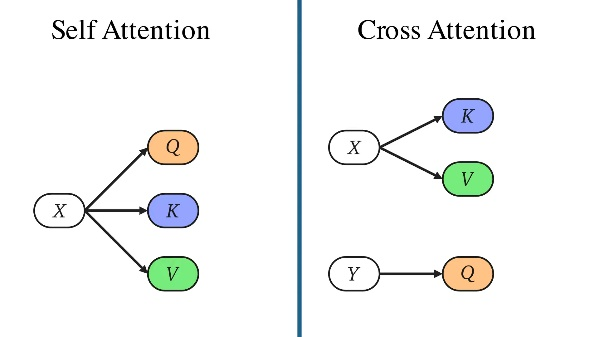
\includegraphics[width=0.55\textwidth]{./appunti_images/media/image89.jpeg}
\caption{Self-Attention vs Cross-Attention. Nella self-attention, Q, K, V provengono tutti dallo stesso input $X$. Nella cross-attention, K e V provengono dall'input $X$, mentre Q proviene da un altro array (i latenti $L$ nel Perceiver).}
\label{fig:self-vs-cross-att}
\end{figure}

\begin{center}
\begin{tabular}{@{}lll@{}}
\toprule
\textbf{Aspetto} & \textbf{Transformer (Self-Att)} & \textbf{Perceiver (Cross-Att)} \\
\midrule
Sorgente Q & Input $X$ ($M$ token) & Latenti $L$ ($N$ latenti) \\
Sorgente K, V & Input $X$ ($M$ token) & Input $X$ ($M$ token) \\
Matrice attenzione & $M \times M$ (quadrata) & $N \times M$ (rettangolare) \\
Complessità & $O(M^2)$ & $O(MN)$, con $N \ll M$ \\
\bottomrule
\end{tabular}
\end{center}

I \textbf{latenti} sono \emph{parametri appresi} (inizializzati come learned position encodings, cfr.\ Appendice C del paper), non uno stato che dipende dall'esempio di input come accade in un RNN. Diventano però analoghi a uno stato ricorrente a causa delle $T$ iterazioni con \emph{weight sharing}: lo stesso modulo cross-attention + latent transformer viene riapplicato più volte ai latenti, in modo simile a un RNN che srotola il proprio passo nel tempo. A differenza di un RNN, però, a ogni iterazione i latenti accedono all'intero input simultaneamente, non a un elemento alla volta.

\begin{figure}[h!]
\centering
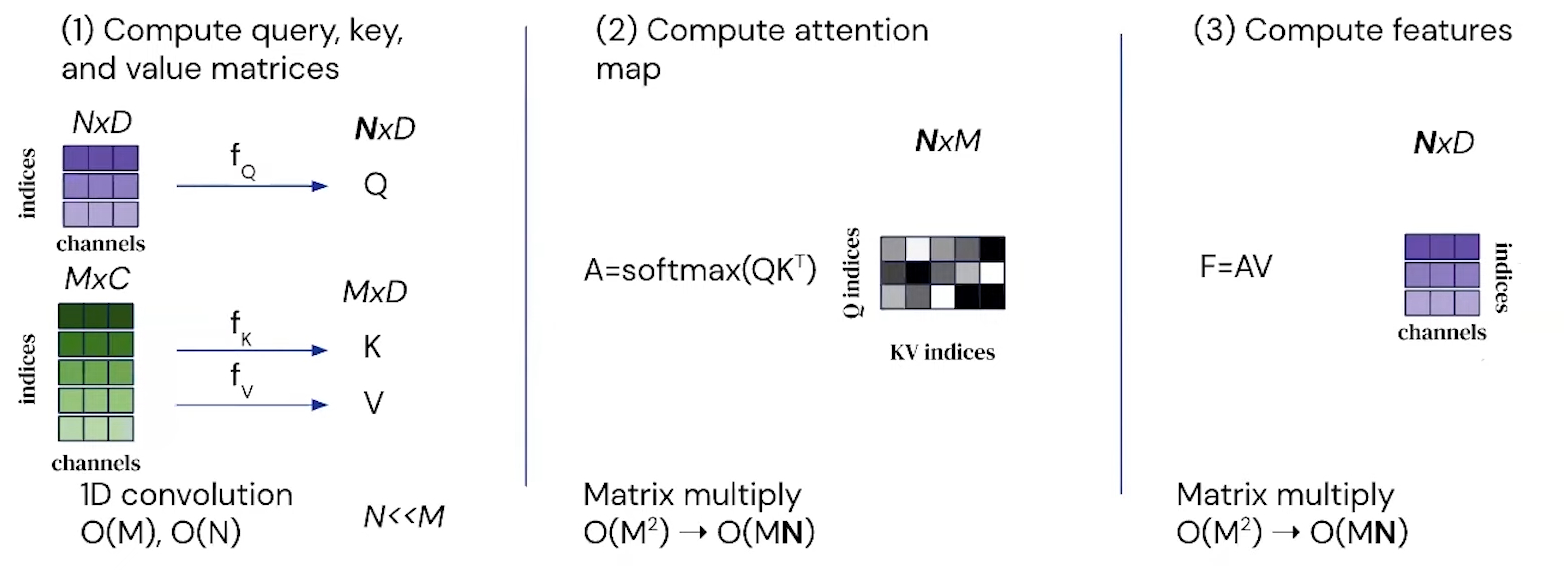
\includegraphics[width=0.85\textwidth]{./appunti_images/media/image43.png}
\caption{Schema della cross-attention nel Perceiver (vista d'insieme dei 3 step). Le singole fasi vengono analizzate in dettaglio di seguito.}
\end{figure}

Rispetto al concetto tradizionale dei Transformer:
\begin{itemize}
\item \textbf{Input}: $M \times C$; come nei Transformer con $M$ numero di unità di input e $C$ dimensione dell'embedding.
\item \textbf{Latenti}: $N \times D$; introdotti dal Perceiver, dove $N$ è il numero di latenti e $D$ la dimensione di ciascun latente.
\end{itemize}

\begin{itemize}
\item \textbf{Query (Q)} $N \times D$: le query provengono dai latenti, di numero fisso $N$, indipendentemente dalla dimensione dell'input $M$. Avere $N$ diverso da $M$ consente di mantenere la complessità computazionale gestibile, poiché $N \ll M$.
\item \textbf{Key (K) e Value (V)} $M \times D$: derivano direttamente dall'input, che ha $M$ elementi, ognuno con una rappresentazione di dimensione $D$.
\end{itemize}

La complessità dell'attenzione passa da $O(M^2)$ a $O(MN)$, poiché le Query hanno $N$ righe (latenti) e le Key hanno $M$ righe (input), con $N \ll M$.

\subsubsection{Step (1): Calcolo delle matrici Q, K, V}

\begin{figure}[h!]
\centering

\includegraphics[width=0.45\textwidth]{./appunti_images/media/image44.png}
\caption{Step (1) --- Il latent array ($N \times D$) viene proiettato in Q tramite $f_Q$, mentre l'input array ($M \times C$) viene proiettato in K e V tramite $f_K$ e $f_V$. Le proiezioni hanno costo $O(N)$ e $O(M)$. $N \ll M$.}
\end{figure}

Il primo step calcola le matrici Q, K, V da due sorgenti diverse:
\begin{itemize}
\item Le \textbf{Query} vengono dal \textbf{latent array} (viola, $N \times D$): ogni latente ``chiede'' quale parte dell'input gli serve.
\item Le \textbf{Key e Value} vengono dall'\textbf{input array} (verde, $M \times C$): ogni token dell'input ``descrive'' il proprio contenuto.
\end{itemize}

Questo è il punto chiave che distingue il Perceiver dal Transformer standard: Q e K/V \emph{non} provengono dallo stesso array. La matrice di attenzione risultante avrà dimensione $N \times M$ (non $M \times M$).

\subsubsection{Step (2): Calcolo della mappa di attenzione}

\begin{figure}[h!]
\centering

\includegraphics[width=0.35\textwidth]{./appunti_images/media/image45.png}
\caption{Step (2) --- $A = \text{softmax}(QK^\top / \sqrt{d_{QKV}}) \in \mathbb{R}^{N \times M}$: la matrice di attenzione è \emph{rettangolare} ($N$ righe per $M$ colonne), non quadrata ($M \times M$). La complessità scende da $O(M^2)$ a $O(MN)$.}
\end{figure}

Quando viene calcolata la mappa di attenzione, invece di essere all'interno di un unico insieme di dati (come i token di testo in un \hyperref[app:transformer]{Transformer} standard), il Perceiver calcola l'attenzione tra due insiemi distinti: \textbf{i latenti} e \textbf{l'input}. La \hyperref[app:softmax]{softmax} (Appendice~\ref{app:softmax}) trasforma i punteggi $QK^\top/\sqrt{d_{QKV}}$ in pesi non-negativi che sommano a 1 lungo ogni riga. Il risultato: una matrice rettangolare $N \times M$ invece di quadratica $M \times M$, riducendo la complessità da $O(M^2)$ a $O(MN)$ dove $N$ è solitamente molto più piccolo di $M$.

\subsubsection{Step (3): Calcolo delle feature}

\begin{figure}[h!]
\centering

\includegraphics[width=0.30\textwidth]{./appunti_images/media/image46.png}
\caption{Step (3) --- $F = AV \in \mathbb{R}^{N \times d_{QKV}}$: ogni latente ora contiene una media pesata dei Value dell'input, secondo i pesi di attenzione calcolati nello step (2). Complessità: $O(M^2) \to O(MN)$. La dimensione $D$ dei latenti viene raggiunta solo \emph{dopo} la proiezione di output $W_o$ (cfr.\ \S\ref{sec:cross-att}), non qui.}
\end{figure}

Il calcolo delle feature segue lo stesso comportamento: la moltiplicazione $F = AV$ produce un output di dimensione $N \times d_{QKV}$ (es.\ $512 \times 261$ per ImageNet), molto più piccolo rispetto all'input originale $M \times C$ ($50\,176 \times 261$). L'output è indipendente dalla dimensione dell'input, il che rende più facile costruire reti profonde partendo dai latenti.

Queste modifiche portano a due vantaggi fondamentali:
\begin{itemize}
\item \textbf{Complessità lineare rispetto all'input}: il calcolo dell'attenzione diventa $O(MN)$ grazie alla trasformazione della matrice da quadrata ($M \times M$) a rettangolare ($N \times M$).
\item \textbf{Mappatura indipendente dalla dimensione dell'input}: il Perceiver può trattare input molto grandi trasformandoli in una rappresentazione compatta attraverso i latenti, condensando informazioni complesse in una forma gestibile.
\end{itemize}

\clearpage
\subsection{Architettura}
\label{sec:architettura}

L'idea centrale del Perceiver è separare la dimensione dei dati in ingresso dalla capacità espressiva della rete. Un input arbitrariamente grande --- un'immagine, un segnale audio, un point cloud, un testo byte-level --- viene prima proiettato in un \textbf{latent array} di dimensione fissa $N \ll M$, e solo su questo array la rete svolge la sua elaborazione profonda. Ne conseguono due proprietà che definiscono l'architettura: lo stesso modello gestisce modalità molto diverse senza modifiche, e la profondità della rete non è più vincolata dalla lunghezza dell'input.

L'elaborazione si snoda in tre stadi. Un \textbf{encoder a cross-attention} legge l'input $X \in \mathbb{R}^{M \times C_{\text{tot}}}$ e lo comprime nel latent array $L \in \mathbb{R}^{N \times D}$. Un \textbf{latent transformer} raffina $L$ applicando self-attention profonda, interamente nello spazio compresso. Una \textbf{testa di pooling e classificazione} aggrega infine i latenti e produce i logit. In questa sezione ne vediamo la struttura d'insieme; i dettagli algoritmici di ciascun blocco sono sviluppati nel Forward Pass (\S\ref{sec:forward-pass}).

\begin{figure}[h!]
\centering

\includegraphics[width=\textwidth]{./appunti_images/media/image47.png}
\caption{Architettura del Perceiver: il Byte Array ($M \times C$) entra da sinistra, viene letto dal Latent Array ($N \times D$) tramite Cross-Attention, poi i latenti vengono raffinati dal Latent Transformer, e infine mediati (Average + Project) per produrre i Logits. I pesi possono essere condivisi tra le iterazioni $T$ (linea tratteggiata in alto).}
\label{fig:arch-forward}
\end{figure}

La Figura~\ref{fig:arch-forward} illustra il flusso dei dati da sinistra verso destra. L'input grezzo --- ad esempio un'immagine $224 \times 224$ --- viene srotolato in un \emph{byte array} di forma $M \times C$ e arricchito con Fourier features posizionali, ottenendo una matrice $M \times C_{\text{tot}}$. Questa matrice entra nel blocco di \textbf{cross-attention}, che agisce in modo asimmetrico: le Query sono prodotte dai latenti (sono solo $N$, poche), mentre Key e Value provengono dall'input (sono $M$, molte). La matrice di attenzione risulta rettangolare $N \times M$ e il costo scende da $O(M^2)$ a $O(MN)$, rendendo trattabile l'elaborazione di input ad altissima dimensionalità.

Il latent array così popolato passa al \textbf{latent transformer}, una pila di $L$ blocchi di self-attention che operano interamente nello spazio compresso e raffinano iterativamente la rappresentazione. L'intero modulo cross-attention + latent transformer viene poi ripetuto $T$ volte: come indicato dalla linea tratteggiata in alto nella figura, i pesi possono essere condivisi tra le iterazioni, e in quel caso il modello si comporta come un RNN che affina lo stesso stato latente ad ogni passo. Al termine, un \textbf{global average pooling} sui latenti produce un vettore di dimensione $D$, che un classificatore lineare proietta nei logit delle classi.

La tabella seguente riassume i valori di questi iperparametri ($N$, $D$, $M$, $T$, $L$, $H$, $d_k$) nella configurazione ImageNet del paper originale (Jaegle et al., 2021).

\begin{table}[h!]
\centering
\caption{Iperparametri del Perceiver per ImageNet (Jaegle et al., 2021, \S4.1 + App.\ C).}
\begin{tabular}{@{}llp{6.5cm}@{}}
\toprule
\textbf{Simbolo} & \textbf{Valore} & \textbf{Descrizione} \\
\midrule
\multicolumn{3}{@{}l}{\emph{Dimensioni globali}} \\
$N$ & 512 & Numero di latenti \\
$D$ & 1024 & Dimensione di ciascun latente \\
$M$ & 50\,176 & Numero di pixel ($224 \times 224$) \\
$C$ & 3 & Canali RGB \\
$C_{\text{tot}}$ & 261 & $C + d(2K+1) = 3 + 258$ (canali + Fourier features) \\
$K$ & 64 & Bande di frequenza per asse \\
\midrule
\multicolumn{3}{@{}l}{\emph{Iterazioni e profondità}} \\
$T$ & 8 & Iterazioni (cross-att + latent transformer) \\
$\ell$ & 6 & Layer di self-attention per blocco del latent transformer \\
\midrule
\multicolumn{3}{@{}l}{\emph{Cross-attention (encoder: input $\to$ latenti)}} \\
$H_{\text{cross}}$ & 1 & Numero di teste (single-head, App.\ C) \\
$d_{\text{QKV}}$ & 261 & Dim.\ di Q, K, V $= \min(D, C_{\text{tot}})$ \\
\midrule
\multicolumn{3}{@{}l}{\emph{Self-attention (latent transformer)}} \\
$H_{\text{self}}$ & 8 & Numero di teste \\
$d_{\text{head}}$ & 128 & Dim.\ per testa $= D/H_{\text{self}}$ \\
\bottomrule
\end{tabular}
\end{table}

\pipeline{0}

\needspace{4\baselineskip}
\subsection{Forward Pass}
\label{sec:forward-pass}

Il \textbf{forward pass} traccia in dettaglio come i dati attraversano l'architettura descritta in \S\ref{sec:architettura} (Figura~\ref{fig:arch-forward}), dalla preparazione dell'input fino ai logit. Il \textbf{backward pass} (\S\ref{sec:backward}) ripercorre lo stesso cammino in senso inverso per calcolare i gradienti e aggiornare i pesi. In questa sezione seguiamo la pipeline step-by-step, evidenziando nel riquadro sottostante lo step corrente.

Il forward pass trasforma un input di dimensione arbitraria ($M$ elementi) in una classificazione, passando attraverso uno spazio latente compatto ($N$ elementi, con $N \ll M$).

Il processo si articola in due fasi principali:
\begin{enumerate}
\item \textbf{Preparazione dell'input}: l'immagine grezza viene trasformata in un byte array arricchito con informazioni posizionali (\hyperref[app:fourier]{Fourier features}), producendo una matrice $M \times C_{\text{tot}}$.
\item \textbf{Elaborazione nel latent space}: un latent array appreso ($N \times D$) interroga l'input tramite \hyperref[sec:cross-att]{cross-attention}, poi viene raffinato iterativamente dal \hyperref[sec:latent-transformer]{latent transformer}. Infine, i latenti vengono mediati (pooling) e classificati.
\end{enumerate}

Di seguito analizziamo ogni step della pipeline, evidenziando nel riquadro sottostante lo step corrente:

\needspace{3\baselineskip}
\subsubsection{Immagine di Input (Byte Array)}

\pipeline{1}

L'input, rappresentato come un byte array
\(M \times C\), rappresenta un modo uniforme per gestire input
eterogenei, indipendentemente dalla loro origine o modalità (immagini,
testo, audio, ecc.).

Nel caso studiato per \textbf{ImageNet} abbiamo un'immagine RGB di
dimensione \(224\  \times 224\) questa verrà processata:

\begin{itemize}
\item
  Ogni pixel dell'immagine è rappresentato da tre valori
  (canali RGB), quindi l'immagine può essere vista come
  una matrice di dimensioni
  \(\left\lbrack \mathbf{224\  \times 224} \right\rbrack\left( \mathbf{M} \right)\mathbf{\times \lbrack 3\rbrack\ (C)}\ \)
\item
  Il numero totale di pixel sarà
  \(\left\lbrack \mathbf{224\  \times 224} \right\rbrack\mathbf{= 50176}\)
\item
  Il numero totale di valori (byte) sarà
  \(\left\lbrack \mathbf{224\  \times 224} \right\rbrack\mathbf{\  \times}\left\lbrack \mathbf{3} \right\rbrack\mathbf{= 150528}\)
\end{itemize}

L'immagine viene convertita in un array lineare o
"appiattito" (semplice \textbf{reshape} della griglia di pixel in una sequenza).

Ogni pixel (con i suoi 3 canali RGB) dell'immagine viene linearizzato e
questa viene trasformata in un array monodimensionale di lunghezza
\(150528\)

\[
\text{Byte Array} = \left[ r_1, g_1, b_1, r_2, g_2, b_2, \ldots, r_{224\times224}, g_{224\times224}, b_{224\times224} \right]
\]

\begin{figure}[htbp]
\centering

\includegraphics[width=0.40\textwidth]{./appunti_images/media/image52.png}
\caption{Il byte array ($M \times C$): ogni riga è un pixel con $C$ canali. Da questo array vengono generate le matrici Key (K) e Value (V) per la cross-attention.}
\end{figure}

\FloatBarrier

\begin{notabox}[title={\textbf{Checkpoint dimensioni --- fine \S1.4.1}}]
A questo punto abbiamo l'immagine cruda organizzata come matrice:

\medskip
\begin{center}
\begin{tabular}{@{}llll@{}}
\toprule
\textbf{Oggetto} & \textbf{Forma simbolica} & \textbf{ImageNet} & \textbf{Contenuto di una riga} \\
\midrule
Byte array (grezzo) & $M \times C$ & $50\,176 \times 3$ & R, G, B del pixel \\
\bottomrule
\end{tabular}
\end{center}

\medskip
Dove $M = 224 \times 224 = 50\,176$ è il numero totale di pixel e $C = 3$ sono i canali RGB.

\medskip
È solo il contenuto ``cromatico'' dei pixel. \textbf{Manca l'informazione posizionale}: questo byte array da solo, dato al Perceiver, non distinguerebbe due immagini che differiscono solo per una permutazione dei pixel. La prossima sezione aggiunge la posizione tramite Fourier features.
\end{notabox}

\needspace{3\baselineskip}
\subsubsection{Positional Encoding (Fourier Features)}
\label{app:fourier}

\pipeline{2}

\textbf{Nota bene:} Il Perceiver \textbf{non lavora direttamente solo con i
3 canali RGB}, ma arricchisce \textbf{ciascun pixel con informazioni} \textbf{di
posizione (x,y)}. Infatti, un pixel con valore {[}R,G,B{]} contiene solo
informazione di colore, ma \textbf{non contiene informazione di
posizione} (es: ``questo rosso è in alto a sinistra o in basso a
destra?''). Senza posizione, il modello non potrebbe distinguere due
immagini identiche ma traslate.

Per fare ciò utiliziamo le \textbf{Fourier Features.} Queste sono una
tecnica di mappatura che trasforma un input scalare o vettoriale
\(x\  \in \mathbb{R}^{d}\) in uno spazio a dimensionalità più alta,
applicando funzioni seno e coseno a frequenze multiple.

Formalmente, data una matrice di frequenze
\(B\  \in \mathbb{R}^{m \times d}\), la mappatura delle Fourier features
è definita come:

\[
\gamma(x) = \left[ \cos(\pi B x),\; \sin(\pi B x) \right] \in \mathbb{R}^{2m}
\]dove:

\begin{itemize}
\item
  \(x\) è il vettore di input (d-dimensionale),
\item
  \(B\) contiene i vettori di frequenze (scelti in modo deterministico o
  campionati da una distribuzione, ad esempio gaussiana),
\item
  il risultato è un embedding di dimensione 2m, in cui ogni componente
  dell'input viene rappresentato tramite combinazioni sinusoidali a
  diverse scale.
\end{itemize}

Sia \((x,y)\) la posizione normalizzata di un pixel (tipicamente in
\(\lbrack - 1,1\rbrack \text{ o } \lbrack 0,1\rbrack\) ).\\
Per una serie di frequenze \(f_{1},f_{2},\ldots,f_{L}\), calcoliamo:

\[\begin{matrix}
\phi(x) = \left\lbrack \sin\left( f_{1}\pi x \right),\cos\left( f_{1}\pi x \right),\ldots,\sin\left( f_{L}\pi x \right),\cos\left( f_{L}\pi x \right) \right\rbrack \\

\end{matrix}\]

\[\phi(y) = \left\lbrack \sin\left( f_{1}\pi y \right),\cos\left( f_{1}\pi y \right),\ldots,\sin\left( f_{L}\pi y \right),\cos\left( f_{L}\pi y \right) \right\rbrack\]

Le frequenze $f_k$ sono \textbf{linearly spaced} tra $1$ e $\mu/2$, dove $\mu/2$ è la \textbf{frequenza di Nyquist} corrispondente al sampling rate di riferimento $\mu$ (Jaegle et al., 2021, \S3.2 e App.\ D). Per ImageNet $224 \times 224$: $\mu = 224$ e $\mu/2 = 112$. Le basse frequenze catturano posizioni globali (``metà sinistra vs.\ destra''), le alte frequenze catturano posizioni precise fino al limite di Nyquist.

\begin{formulabox}[title={\textbf{Calcolo di $C$: perché 261 e non 3}}]

\textbf{Formula dal paper} (Jaegle et al., 2021, \S3.2 + App.\ D):

Per ogni dimensione spaziale $d$, il Perceiver costruisce un vettore posizionale concatenando le Fourier features con la \textbf{coordinata grezza} $x_d$:

\[
\text{PE}(x_d) = \Big[\; \underbrace{\sin(f_1 \pi\, x_d),\; \cos(f_1 \pi\, x_d),\; \ldots,\; \sin(f_K \pi\, x_d),\; \cos(f_K \pi\, x_d)}_{2K \text{ valori sinusoidali}},\;\; \underbrace{x_d}_{1 \text{ coordinata grezza}} \;\Big]
\]

dove:
\begin{itemize}
\item $x_d \in [-1, 1]$ è il \textbf{valore grezzo della coordinata} lungo la dimensione $d$, normalizzato nell'intervallo $[-1,1]$. Per un'immagine 2D: $x_1 = x$ (posizione orizzontale), $x_2 = y$ (posizione verticale).
\item $f_k$, $k = 1, \ldots, K$, sono le frequenze, \textbf{linearly spaced tra $1$ e $\mu/2$} (Nyquist del sampling rate di riferimento). Per ImageNet: $\mu/2 = 112$.
\item $K$ è il numero di bande di frequenza per asse (nel paper: $K = 64$).
\end{itemize}

\textbf{Perché concatenare la coordinata grezza $x_d$?}

Le Fourier features ($\sin$/$\cos$) sono \textbf{periodiche}: frequenze alte possono mappare posizioni diverse nello stesso valore. Concatenando il valore grezzo $x_d$ (che è \emph{unico} per ogni posizione), il modello ha sempre accesso alla posizione esatta, senza ambiguità. Le sinusoidi forniscono sensibilità multi-scala, il valore grezzo fornisce l'identità posizionale.

\medskip
\textbf{Calcolo per un'immagine 2D} con $d=2$ assi e $K=64$ bande:

\textbf{Per ogni asse}: $2K + 1 = 2 \times 64 + 1 = 129$ valori (128 sinusoidi + 1 coordinata grezza).

\textbf{Con $d=2$ assi} (x e y): $d \times (2K+1) = 2 \times 129 = 258$ valori posizionali.

\textbf{Sommati ai 3 canali RGB}:

\[
C_{\text{tot}} = \underbrace{3}_{\text{RGB}} + \underbrace{d \times (2K + 1)}_{2 \times 129 = 258 \text{ Fourier + coord. grezze}} = \mathbf{261}
\]

Ogni pixel diventa un vettore di 261 valori:

\[
\Big[\; R,\, G,\, B,\;\; \underbrace{x_1,\; \sin(f_1 \pi\, x_1),\; \cos(f_1 \pi\, x_1),\; \ldots,\; \cos(f_{64} \pi\, x_1)}_{129 \text{ per asse } x},\;\; \underbrace{x_2,\; \sin(f_1 \pi\, x_2),\; \ldots,\; \cos(f_{64} \pi\, x_2)}_{129 \text{ per asse } y} \;\Big]
\]
\end{formulabox}

\begin{notabox}[title={\textbf{Esempio concreto: un pixel in posizione $(0.3, 0.7)$ con colore rosso}}]
\begin{itemize}
\item Canali RGB: $[255, 0, 0]$ (normalizzati: $[1.0, 0, 0]$)
\item Posizione normalizzata: $(x, y) = (0.3, 0.7)$
\item Fourier per $x=0.3$ con 3 frequenze illustrative ($f_1=1, f_2=2, f_3=4$, scelte per comodità di calcolo; il paper ne usa 64 linearly spaced tra 1 e 112):

\[
[0.3,\; \sin(0.3\pi),\; \cos(0.3\pi),\; \sin(0.6\pi),\; \cos(0.6\pi),\; \sin(1.2\pi),\; \cos(1.2\pi),\; \ldots]
\]
\[
= [0.3,\; 0.809,\; 0.588,\; 0.951,\; -0.309,\; -0.588,\; 0.809,\; \ldots]
\]
\item Analogamente per $y=0.7$
\item Vettore finale: $[1.0, 0, 0, \underbrace{0.3, 0.809, 0.588, \ldots}_{129}, \underbrace{0.7, \ldots}_{129}] \in \mathbb{R}^{261}$
\end{itemize}
Perché \textbf{concatenare} e non sommare? Perché la concatenazione preserva l'informazione di colore e posizione separatamente, mentre la somma la mescolerebbe in modo ambiguo. Il Perceiver usa la concatenazione (a differenza dei Transformer per il linguaggio che sommano il positional encoding).
\end{notabox}

\begin{notabox}[title={\textbf{Perché non le frequenze di NeRF ($f_k = 2^k$)?}}]
NeRF (Mildenhall et al., 2020) usa frequenze \textbf{esponenziali} $f_k = 2^k$, mentre il Perceiver le prende linearly spaced tra $1$ e $\mu/2$. Il paper giustifica esplicitamente la scelta (App.\ D):

``\emph{la parametrizzazione NeRF produce frequenze molto alte anche con un numero moderato di bande --- ad esempio la $64$-esima banda avrebbe frequenza $2^{64} \approx 1.8 \times 10^{19}$}''.

Con $K = 64$ bande, NeRF porterebbe a valori numerici del tutto incompatibili con la precisione in virgola mobile. Il paper riporta inoltre \textbf{instabilità di training} già oltre $k \approx 15$ bande con la parametrizzazione esponenziale. Lo spacing lineare evita il problema perché, aggiungendo bande, si campiona più densamente lo spettro nel range $[1, \mu/2]$ anziché salire indefinitamente. Nel codice di progetto (\texttt{src/utils/positional\_encoding.py}) le frequenze sono ottenute con \texttt{torch.linspace}, coerentemente col paper.
\end{notabox}

Quindi il Byte Array finale ha dimensione:

\[
\text{Byte Array} \in \mathbb{R}^{M \times C_{\text{tot}}} = \mathbb{R}^{50176 \times 261}
\]

\begin{notabox}[title={\textbf{Checkpoint dimensioni --- fine \S1.4.2}}]
Dopo l'aggiunta delle Fourier features, ogni pixel è descritto da $C_{\text{tot}} = 261$ numeri invece di $C = 3$:

\medskip
\begin{center}
\begin{tabular}{@{}llll@{}}
\toprule
\textbf{Oggetto} & \textbf{Forma simbolica} & \textbf{ImageNet} & \textbf{Contenuto di una riga} \\
\midrule
Byte array (grezzo) & $M \times C$ & $50\,176 \times 3$ & RGB \\
\textbf{Byte array (con Fourier PE)} $X$ & $\boldsymbol{M \times C_{\text{tot}}}$ & $\mathbf{50\,176 \times 261}$ & $3$ RGB $+$ $258$ Fourier \\
\bottomrule
\end{tabular}
\end{center}

\medskip
Le costanti simboliche:
\begin{itemize}\setlength\itemsep{0.1em}
\item $M$ = numero di elementi di input ($50\,176$ per ImageNet)
\item $C$ = canali originali ($3$ per RGB)
\item $C_{\text{tot}} = C + d\,(2K + 1)$: canali totali dopo Fourier, con $d$ = numero di dimensioni spaziali (2 per immagini) e $K$ = numero di bande di frequenza (64 per ImageNet, paper §4.1)
\item Per ImageNet: $C_{\text{tot}} = 3 + 2 \cdot (2 \cdot 64 + 1) = 3 + 258 = 261$
\end{itemize}

\medskip
Da qui in avanti, quando si scrive ``byte array'' si intende la versione arricchita $X \in \mathbb{R}^{M \times C_{\text{tot}}}$. I valori posizionali rendono il Perceiver capace di distinguere tra due immagini che differiscono per una permutazione dei pixel (cfr.\ Tab.\ 2 del paper).
\end{notabox}

\needspace{3\baselineskip}
\subsubsection{Proiezione Lineare Input}

\pipeline{3}

\textbf{Proiezione Lineare $C_{\text{tot}} = 261 \to D = 1024$}

Nel paper originale, le proiezioni $K$ e $V$ nella cross-attention vengono applicate \textbf{direttamente} dal byte array ($C=261$) allo spazio delle chiavi ($d_k$). Tuttavia, in alcune implementazioni si usa una proiezione lineare intermedia $C_{\text{tot}} \to D$ per uniformare le dimensioni:

\begin{formulabox}[title={\textbf{Proiezione lineare dell'input (non nel paper originale)}}]
Nell'\textbf{implementazione del paper} (Jaegle et al., 2021, App.\ C) \emph{non} esiste una proiezione intermedia $C_{\text{tot}} \to D$: le matrici $W_K, W_V$ proiettano direttamente dal byte array $\mathbb{R}^{50176 \times 261}$ a dimensione $d_{QKV} = \min(D, C_{\text{tot}}) = 261$.

Alcune implementazioni (e.g., il nostro codice di progetto) scelgono invece di proiettare l'input a $H \cdot d_{\text{head}}$, per uniformare il flusso multi-head. Nel nostro codice $H = 8$ e $d_{\text{head}} = 64$, quindi:
\[
W_{\text{embed}} \in \mathbb{R}^{C_{\text{tot}} \times (H \cdot d_{\text{head}})},\qquad x \in \mathbb{R}^{261} \longrightarrow x_{\text{embed}} \in \mathbb{R}^{512}
\]
La dimensione finale del latente $D = 1024$ viene raggiunta \emph{dopo} l'attention, tramite la proiezione di output $W_o \in \mathbb{R}^{512 \times 1024}$ che riporta lo spazio a $D$ per la \hyperref[app:residual]{residual connection} (Appendice~\ref{app:residual}) con i latenti.

\textbf{Riepilogo delle dimensioni intermedie per ImageNet:}
\begin{itemize}
\item \textbf{Paper}: $d_{QKV} = 261$, poi $W_o: 261 \to 1024$.
\item \textbf{Nostro codice}: $d_{QKV} = 512$, poi $W_o: 512 \to 1024$.
\item In \emph{entrambi i casi}, la dimensione $1024$ non compare \emph{dentro} l'attention: è solo la dim dei latenti (input Q) e la dim di output dopo $W_o$.
\end{itemize}
\end{formulabox}

\begin{notabox}[title={\textbf{Checkpoint dimensioni --- fine \S1.4.3}}]
A questo punto del forward pass abbiamo una sola matrice, l'input pronto per la cross-attention:

\medskip
\begin{center}
\begin{tabular}{@{}llll@{}}
\toprule
\textbf{Oggetto} & \textbf{Forma simbolica} & \textbf{ImageNet} & \textbf{Fonte} \\
\midrule
Byte array $X$ & $M \times C_{\text{tot}}$ & $50\,176 \times 261$ & RGB ($3$) $+$ Fourier PE ($258$) \\
\bottomrule
\end{tabular}
\end{center}

\medskip
\textbf{Perché restiamo a $261$ e non saliamo a $1024$?}

La tentazione sarebbe di ``uniformare'' subito il byte array alla dimensione dei latenti ($D = 1024$), ma \emph{il paper non lo fa}. Il motivo è che la cross-attention che segue userà come dimensione interna il minimo tra le due sorgenti, $d_{QKV} = \min(D, C_{\text{tot}}) = \min(1024, 261) = 261$ (cfr.\ App.\ C del paper). Espandere l'input a $1024$ solo per poi ricomprimerlo a $261$ dentro la cross-attention sarebbe uno spreco di parametri e di FLOPs: i $261$ valori per pixel contengono già tutta l'informazione utile (colore + posizione), aumentare la dimensione non aggiunge nulla. Formalmente, una proiezione lineare $261 \to 1024$ ha \emph{rango} $\le 261$: produrrebbe $1024$ feature ma solo $261$ linearmente indipendenti (le altre ridondanti). Espandere non può \emph{creare} informazione che non c'è.

Il nostro codice fa invece una proiezione a $H \cdot d_{\text{head}} = 512$ perché adotta multi-head ($H=8, d_{\text{head}}=64$) anche nella cross-attention: in quel caso $d_{QKV}$ è forzato dalla scelta delle teste, non dal minimo degli input. Ma è una divergenza implementativa, non una necessità del paper.

\medskip
\textbf{Cosa arriva adesso.} La prossima sezione (\S\ref{sec:latent-array}) introduce il \emph{latent array} $L$, la seconda matrice che serve alla cross-attention; poi \S\ref{sec:cross-att} combina $X$ e $L$ producendo $Q, K, V$ --- aggiungeremo quelle righe al checkpoint.
\end{notabox}

\needspace{3\baselineskip}
\subsubsection{Latent Array}
\label{sec:latent-array}

\pipeline{4}

È una \textbf{matrice di vettori latenti} \(L \in R^{N \times D}\ \)
\textbf{interamente appresa} (parametri del modello).

\begin{itemize}
\item
  \textbf{N} = numero di latenti (slot/ ``unità di memoria'').
\item
  \textbf{D} = dimensione del canale/embedding dei latenti
\end{itemize}

Questi vettori \textbf{non derivano} direttamente dall'input e
\textbf{non hanno un legame spaziale} con token/pixel specifici:
\textbf{sono una base compatta che il modello usa per \textbf{riassumere}
l'input}.

Nel caso specifico del Perceiver per ImageNet, l'array
latente è \(N = 512\ \)(\(N \ll M(\mathbf{50176)}\)) e \(D = 1024\).

L'array latente \(L \in \mathbb{R}^{512 \times 1024}\)
(per ImageNet) è inizializzato campionando ciascun elemento da una
distribuzione:

\[L_{ij} \sim \mathcal{N}\left( 0,{0.02}^{2} \right),\ \text{ troncata a}\lbrack - 2,2\rbrack.\]

\[
L = \begin{bmatrix}
 0.012  & -0.004 &  0.021 & \cdots & -0.017 \\
-0.009  &  0.015 &  0.003 & \cdots &  0.008 \\
 0.020  &  0.001 & -0.014 & \cdots &  0.027 \\
\vdots  & \vdots & \vdots & \ddots & \vdots \\
-0.006  &  0.022 & -0.010 & \cdots &  0.004
\end{bmatrix}_{512 \times 1024}
\]In
pratica i numeri dentro \(L\) sono quasi tutti piccolissimi, tipicamente
compresi fra -0.05 e +0.05 (perché la gaussiana è molto stretta attorno
a 0 ).\\
Il troncamento a \(\lbrack - 2,2\rbrack\) esiste per sicurezza, ma
\(con\ \sigma = 0.02\) è rarissimo che si producano valori oltre 0.1 -
quindi quasi mai entra davvero in gioco.\\
Questi numeri sono i vettori di partenza dei 512 slot latenti: ognuno è
un vettore di 1024 valori inizializzati così.

\textbf{Perché?}

\begin{itemize}
\item
  \textbf{Evitare gradienti instabili}: se i latenti partissero con
  valori grandi, i prodotti \(QK^{T}\ \)sarebbero enormi, la softmax
  saturerebbe, e i gradienti diventerebbero instabili.
\item
  \textbf{Garantire neutralità}: media zero significa che nessun latente
  ha un ``vantaggio'' iniziale su un altro.
\item
  \textbf{Sicurezza numerica}: il troncamento assicura che non ci siano
  valori anomali che potrebbero falsare il training nelle prime epoche.
\item
  \textbf{Permettere specializzazione graduale}: partendo con valori
  piccoli e neutri, i latenti vengono ``riempiti'' progressivamente
  dall'informazione dell'input, e col tempo ciascuno si specializza
  (bordo, colore, texture, pattern globali\ldots).
\end{itemize}

\begin{figure}[h!]
\centering

\includegraphics[width=0.45\textwidth]{./appunti_images/media/image60.png}
\caption{Latent array ($N \times D$): matrice appresa che genera le Query (Q) per la cross-attention.}
\end{figure}

\begin{notabox}[title={\textbf{Checkpoint dimensioni --- fine \S1.4.4}}]
Adesso abbiamo i due array che la cross-attention metterà in comunicazione:

\medskip
\begin{center}
\begin{tabular}{@{}llll@{}}
\toprule
\textbf{Oggetto} & \textbf{Forma simbolica} & \textbf{ImageNet} & \textbf{Natura} \\
\midrule
Byte array $X$ & $M \times C_{\text{tot}}$ & $50\,176 \times 261$ & input ($3$ RGB $+$ $258$ Fourier) \\
\textbf{Latent array} $\boldsymbol{L}$ & $\boldsymbol{N \times D}$ & $\mathbf{512 \times 1024}$ & parametri appresi, init $\mathcal{N}(0, 0.02^2)$ troncata \\
\bottomrule
\end{tabular}
\end{center}

\medskip
Le nuove costanti simboliche:
\begin{itemize}\setlength\itemsep{0.1em}
\item $N$ = numero di latenti ($512$ per ImageNet, paper §4.1)
\item $D$ = dimensione di ciascun latente ($1024$ per ImageNet, paper §4.1)
\item Vincolo fondamentale: $N \ll M$ (qui $N/M = 512/50\,176 \approx 1\%$), è ciò che permette la riduzione da $O(M^2)$ a $O(MN)$
\end{itemize}

\medskip
Osservazioni:
\begin{itemize}\setlength\itemsep{0.1em}
\item $L$ non deriva dall'immagine: è un parametro del modello, uguale per tutti gli esempi del batch. Cambia solo durante il training (backward) --- non durante l'inferenza.
\item Le due matrici hanno dimensione-feature \emph{diversa} ($C_{\text{tot}}=261$ vs $D=1024$). Sarà la cross-attention a farle incontrare in uno spazio comune: $d_{QKV} = \min(D, C_{\text{tot}}) = 261$.
\item Il numero di righe è molto diverso ($M = 50\,176$ vs $N = 512$): è questa asimmetria che rende la complessità $O(MN)$ invece di $O(M^2)$.
\end{itemize}

\medskip
Prossimo passo (\S\ref{sec:cross-att}): da $X$ e $L$ otterremo $Q, K, V$.
\end{notabox}

\needspace{3\baselineskip}
\subsubsection{Cross-Attention Block}
\label{sec:cross-att}

\pipeline{5}

\begin{notabox}[title={\textbf{Cross-attention: single-head nel paper, multi-head nel nostro codice}}]
Per ImageNet il paper originale (App.\ C) usa una cross-attention a \textbf{singola testa} ($H_{\text{cross}} = 1$). Q, K, V hanno tutte dimensione $d_{\text{QKV}} = 261$, pari al \emph{minimo} tra i canali dei latenti ($D = 1024$) e quelli dell'input ($C_{\text{tot}} = 261$). L'output dell'attention viene riportato a $D = 1024$ tramite una proiezione finale $W_o \in \mathbb{R}^{261 \times 1024}$, così da poterlo sommare residualmente ai latenti.

Il nostro codice di progetto (\texttt{src/perceiver/attention.py}, classe \texttt{CrossAttention}) adotta invece una convenzione più standard, con cross-attention \textbf{multi-head} ($H = 8$, $d_{\text{head}} = 64$, totale $512$). È una scelta legittima e più simile alla pratica corrente, ma \emph{diverge dal paper}: quando si descrive l'architettura originale occorre tenere presente la distinzione.

Nel seguito di questa sezione descriviamo la formulazione della cross-attention usando $d_k$ come dimensione generica di proiezione; il valore esatto ($261$ nel paper, $64$ per testa nel nostro codice) dipende dal setting.
\end{notabox}

\begin{figure}[h!]
\centering

\includegraphics[width=0.45\textwidth]{./appunti_images/media/image44.png}
\caption{Step (1) del blocco: calcolo delle matrici $Q$, $K$, $V$. Le Query provengono dal latent array ($N \times D$), le Key e Value dall'input array ($M \times C_{\text{tot}}$). $N \ll M$.}
\end{figure}

\paragraph{Cosa deve fare il blocco.} La cross-attention deve permettere agli $N$ latenti di ``leggere'' informazione dai $M$ elementi dell'input byte array. Concretamente: ciascun latente emette una \emph{Query} (una domanda: ``cosa sto cercando?''), ogni elemento dell'input produce una \emph{Key} (una descrizione: ``io rappresento questo'') e un \emph{Value} (un contenuto informativo effettivo). Il blocco calcola la compatibilità tra ogni query e ogni key, la trasforma in una distribuzione di probabilità tramite softmax, e la usa per aggregare i value in un nuovo latente.

\paragraph{Punto di partenza: due array da armonizzare.} All'ingresso del blocco abbiamo due matrici di forme molto diverse:

\begin{itemize}\setlength\itemsep{0.2em}
\item Il \textbf{byte array} $X \in \mathbb{R}^{50176 \times 261}$ (un'immagine ImageNet dopo aver concatenato RGB + Fourier features: $50\,176$ pixel, $261$ valori ciascuno).
\item Il \textbf{latent array} $L \in \mathbb{R}^{512 \times 1024}$ (parametri appresi del modello: $512$ latenti di dimensione $1024$).
\end{itemize}

Le due matrici vivono in spazi di dimensione differente ($261$ vs $1024$): \emph{prima} di calcolare Q, K, V dobbiamo decidere in quale spazio far incontrare queste due sorgenti.

\paragraph{Passaggio 1: LayerNorm pre-attention.} Il paper (App.\ C) specifica che entrambi gli array, prima delle proiezioni lineari che producono Q, K, V, attraversano una \textbf{LayerNorm} (pattern pre-norm). La LayerNorm è un'operazione \emph{riga per riga}: per ogni pixel del byte array (o per ogni latente) si calcolano media e deviazione standard delle sue feature e si riporta la distribuzione a media $0$ e varianza $1$, poi si applicano due parametri appresi $\gamma$ e $\beta$ per-feature.

\medskip
\textbf{Cosa fa in dettaglio, per ogni riga.} Consideriamo una generica riga $x = (x_1, \ldots, x_F)$ (con $F = 261$ nel byte array, $F = 1024$ nel latente). LayerNorm esegue questi 4 passaggi:

\begin{enumerate}\setlength\itemsep{0.2em}
\item Calcola la \textbf{media} sulla riga:
\[
\mu = \frac{1}{F}\sum_{j=1}^{F} x_j
\]
\item Calcola la \textbf{deviazione standard} sulla riga:
\[
\sigma = \sqrt{\frac{1}{F}\sum_{j=1}^{F} (x_j - \mu)^2}
\]
\item \textbf{Normalizza} ogni elemento: $\hat{x}_j = (x_j - \mu)/(\sigma + \epsilon)$, con $\epsilon \approx 10^{-5}$ per stabilità numerica. Dopo questo step la riga ha media $0$ e varianza $1$ \emph{per costruzione matematica}.
\item Applica \textbf{scale e shift} appresi: $\tilde{x}_j = \gamma_j \cdot \hat{x}_j + \beta_j$, dove $\gamma, \beta \in \mathbb{R}^F$ sono vettori di parametri.
\end{enumerate}

I parametri $\gamma, \beta$ sono \textbf{diversi per ciascuna LayerNorm} del Perceiver (due blocchi distinti: uno sul byte array, uno sul latent array), e sono gli stessi per tutte le righe dentro la stessa LayerNorm (una LN su $50{,}176$ pixel ha un solo vettore $\gamma$ di dim $261$, non $50{,}176$ vettori diversi).

\medskip
\textbf{Dimensioni dei parametri di ciascuna LayerNorm:}

\begin{center}
\begin{tabular}{@{}llll@{}}
\toprule
\textbf{LayerNorm} & \textbf{Input} & \textbf{$\gamma, \beta$} & \textbf{Output} \\
\midrule
$\mathrm{LN}_\text{input}$ (sul byte array) & $\mathbb{R}^{M \times C_{\text{tot}}} = \mathbb{R}^{50176 \times 261}$ & $\mathbb{R}^{261}$ ciascuno & $\mathbb{R}^{50176 \times 261}$ \\
$\mathrm{LN}_\text{latent}$ (sul latent array) & $\mathbb{R}^{N \times D} = \mathbb{R}^{512 \times 1024}$ & $\mathbb{R}^{1024}$ ciascuno & $\mathbb{R}^{512 \times 1024}$ \\
\bottomrule
\end{tabular}
\end{center}

\medskip
\textbf{Perché LayerNorm non cambia le dimensioni:} ogni passaggio sopra (media, standardizzazione, scale, shift) è un'operazione \emph{element-wise} (o per riga) che produce un output di forma identica all'input. La LayerNorm riceve $N \times F$ e restituisce $N \times F$, sempre.

\medskip
\textbf{Risultato finale:}
\[
\tilde{X} = \mathrm{LN}_\text{input}(X) \in \mathbb{R}^{M \times C_{\text{tot}}} = \mathbb{R}^{50176 \times 261}, \qquad \tilde{L} = \mathrm{LN}_\text{latent}(L) \in \mathbb{R}^{N \times D} = \mathbb{R}^{512 \times 1024}
\]

Da qui in avanti, ogni volta che compaiono $X$ e $L$ nelle proiezioni, sono sempre queste versioni normalizzate.

\begin{notabox}[title={\textbf{Perché LayerNorm \emph{prima} dell'attention (pre-norm)?}}]
Il pattern \emph{pre-norm} applica LN \emph{prima} della sotto-funzione (attention o MLP) e somma il risultato al residuo non normalizzato: $y = x + f(\mathrm{LN}(x))$. L'alternativa \emph{post-norm} (del Transformer originale) è $y = \mathrm{LN}(x + f(x))$.

Il pre-norm (usato dal Perceiver e da GPT-2) rende il training più stabile su reti profonde: il residuo $x$ è un percorso ``pulito'' sul quale il gradiente può fluire senza attraversare la LayerNorm, evitando vanishing gradients nei modelli molto deep. È lo stesso motivo per cui il Perceiver preferisce questo schema.

Dettagli e derivazione completa della LayerNorm (forward $+$ backward con la formula a 3 termini $1/(\sigma + \epsilon)$) si trovano in Appendice~\ref{app:layernorm} di questi appunti.
\end{notabox}

\paragraph{Passaggio 2: scelta della dimensione interna dell'attention.} Le matrici $Q$, $K$, $V$ devono avere tutte la \textbf{stessa dimensione-feature} (chiamiamola $d_{QKV}$), altrimenti il prodotto scalare $QK^\top$ non è definito. Il paper (App.\ C, citazione letterale):

\begin{quote}\small
\emph{``The queries, keys, and values have the same number of channels as the minimum of the input channels, which is typically the key/value input (i.e.\ 261 for ImageNet).''}
\end{quote}

Cioè si sceglie:
\[
d_{QKV} = \min(D,\, C_{\text{tot}}) = \min(1024,\, 261) = 261
\]

\textbf{Perché proprio il minimo?} L'argomento è di efficienza. Se il byte array ha già solo $261$ canali, proiettare K e V in una dimensione più grande (es.\ $1024$) non aggiungerebbe informazione: il contenuto informativo per pixel è già ``tutto lì'' in quei $261$ numeri. Espandere sarebbe spreco di parametri e FLOPs. Scegliere il minimo tiene Q, K, V in una dimensione compatta ($261$) e usa $1024$ solo dove serve davvero: come spazio dei latenti e come target di output per poter fare la residual connection (lo vedremo alla fine).

\paragraph{Passaggio 3: calcolo delle Query $Q$ (dai latenti).} Le query partono dai latenti, che vivono in dimensione $D = 1024$. Servono due cose da $W_Q$: accettare un vettore in input di dimensione $1024$, e produrre un output in dimensione $d_{QKV} = 261$. Quindi:
\[
W_Q \in \mathbb{R}^{D \times d_{QKV}} = \mathbb{R}^{1024 \times 261}
\]
Il prodotto riga-per-riga è:
\[
Q = \tilde{L}\, W_Q
\]
dimensionalmente: $(512 \times 1024)\,(1024 \times 261) = (512 \times 261)$. Ogni latente ha prodotto una query di $261$ valori:
\[
\boxed{Q \in \mathbb{R}^{512 \times 261}}
\]
I $512$ restano ($W_Q$ non cambia il numero di latenti), la dimensione-feature scende da $1024$ a $261$.

\paragraph{Passaggio 4: calcolo delle Key $K$ (dall'input).} Le key partono dal byte array, che vive già in dimensione $C_{\text{tot}} = 261$. Servono a $W_K$: accettare un vettore di $261$ valori e produrre un output pure in $d_{QKV} = 261$. Quindi:
\[
W_K \in \mathbb{R}^{C_{\text{tot}} \times d_{QKV}} = \mathbb{R}^{261 \times 261}
\]
Il calcolo:
\[
K = \tilde{X}\, W_K
\]
dimensioni: $(50176 \times 261)\,(261 \times 261) = (50176 \times 261)$:
\[
\boxed{K \in \mathbb{R}^{50176 \times 261}}
\]

\paragraph{Passaggio 5: calcolo dei Value $V$ (dall'input).} Stesso procedimento, diversa matrice di pesi:
\[
W_V \in \mathbb{R}^{261 \times 261}, \qquad V = \tilde{X}\, W_V \in \mathbb{R}^{50176 \times 261}
\]

\paragraph{Perché $W_K$ e $W_V$ sono "quadrate" $261 \times 261$?} Può sembrare inutile: se input e output hanno la stessa dimensione, perché non usare la matrice identità? Perché la trasformazione è \textbf{appresa}: $W_K$ impara a produrre key ``ottimali'' per il matching con le query (es.\ riduce il peso di feature rumorose, mescola canali correlati), e $W_V$ impara a produrre value ``ottimali'' per essere poi pesati dall'attention. La dimensione è la stessa, ma lo \emph{spazio} in cui vivono i 261 numeri è completamente diverso da quello di partenza.

\paragraph{Niente bias nelle proiezioni Q/K/V.} Il paper (App.\ C) descrive le tre proiezioni come ``linear layers'' senza menzionare termini di bias. Il nostro codice conferma (\texttt{nn.Linear(..., bias=False)} in \texttt{src/perceiver/attention.py}, L84--85). Quindi non compare un $+b_Q, +b_K, +b_V$: la trasformazione è esattamente $W x$, non $W x + b$. I bias compaiono invece nei layer successivi ($W_o$, MLP, classificatore finale).

\paragraph{Riepilogo delle forme dopo Passaggio 5.}

\begin{center}
\begin{tabular}{@{}lllll@{}}
\toprule
\textbf{Matrice} & \textbf{Forma simbolica} & \textbf{ImageNet} & \textbf{Viene da} & \textbf{Significato riga} \\
\midrule
$\tilde{L}$ (input Q) & $N \times D$ & $512 \times 1024$ & LN del latent array & un latente \\
$\tilde{X}$ (input K/V) & $M \times C_{\text{tot}}$ & $50\,176 \times 261$ & LN del byte array & un pixel \\
$W_Q$ & $D \times d_{QKV}$ & $1024 \times 261$ & pesi appresi & --- \\
$W_K$ & $C_{\text{tot}} \times d_{QKV}$ & $261 \times 261$ & pesi appresi & --- \\
$W_V$ & $C_{\text{tot}} \times d_{QKV}$ & $261 \times 261$ & pesi appresi & --- \\
\midrule
$Q = \tilde{L} W_Q$ & $N \times d_{QKV}$ & $512 \times 261$ & proiezione latenti & query di un latente \\
$K = \tilde{X} W_K$ & $M \times d_{QKV}$ & $50\,176 \times 261$ & proiezione input & key di un pixel \\
$V = \tilde{X} W_V$ & $M \times d_{QKV}$ & $50\,176 \times 261$ & proiezione input & value di un pixel \\
\bottomrule
\end{tabular}
\end{center}

\textbf{L'asimmetria chiave:} $Q$ ha \emph{poche} righe ($N = 512$) e $K, V$ ne hanno \emph{tante} ($M = 50\,176$). Le colonne sono tutte uguali ($d_{QKV} = 261$). Questa asimmetria è ciò che permette al prodotto $QK^\top$ di essere rettangolare $N \times M = 512 \times 50\,176$ invece di quadrato $M \times M$: è la riduzione di complessità da $O(M^2)$ a $O(MN)$ descritta nella §1.1 (il problema della complessità quadratica).

\begin{notabox}[title={\textbf{Inizializzazione di $W_Q$, $W_K$, $W_V$: Xavier Uniform}}]
Le matrici di peso vengono inizializzate con Xavier Uniform (Glorot \& Bengio, 2010). Formalmente: $W_{ij} \sim U(-a, a)$ con $a = \sqrt{6 / (\mathit{fan}_{in} + \mathit{fan}_{out})}$. Per $W_K: 261 \times 261$: $a = \sqrt{6/522} \approx 0.107$, quindi i pesi iniziali stanno in $[-0.107, +0.107]$. Xavier mantiene la varianza delle attivazioni costante attraverso i layer, evitando che i segnali esplodano o collassino a zero. Dopo l'inizializzazione, i pesi evolvono tramite backpropagation --- solo allora la rete ``impara'' qualcosa.
\end{notabox}

\begin{figure}[h!]
\centering

\includegraphics[width=0.50\textwidth]{./appunti_images/media/image62.png}
\caption{Schema complessivo della cross-attention: il latent array (512 $\times$ 1024) proiettato a $Q$ (512 $\times$ 261) interroga il byte array (50\,176 $\times$ 261) proiettato a $K, V$ (50\,176 $\times$ 261). Il prodotto $QK^\top$ produce una matrice di attenzione rettangolare 512 $\times$ 50\,176.}
\end{figure}


\needspace{4\baselineskip}
\subsubsection{Scaled Dot-Product Attention}
\label{sec:scaled-dot-product}

A questo punto disponiamo di $Q \in \mathbb{R}^{512 \times 261}$ dai latenti e di $K, V \in \mathbb{R}^{50176 \times 261}$ dall'input. Il blocco di \emph{scaled dot-product attention} li combina in quattro operazioni principali (prodotto $QK^\top$, scaling, softmax, aggregazione con $V$), illustrate nello schema che segue.

\begin{figure}[h!]
\centering

\includegraphics[width=0.40\textwidth]{./appunti_images/media/image63.png}
\caption{Pipeline della scaled dot-product attention nel Perceiver: $QK^\top$, scaling per $\sqrt{d_{QKV}}$, softmax per riga, prodotto finale con $V$. Il passo ``Mask'' non viene usato (il Perceiver è non-causale).}
\label{fig:sdpa-pipeline}
\end{figure}

\paragraph{Passaggio 1: prodotto scalare $QK^\top$.} Misuriamo la compatibilità tra ogni query e ogni key calcolandone il prodotto scalare: due vettori allineati producono un numero alto, due vettori in direzioni diverse un numero basso o negativo. In forma matriciale,
\[
\text{Scores} = Q\,K^\top \in \mathbb{R}^{512 \times 50\,176},
\]
dove ogni riga corrisponde a un latente, ogni colonna a un pixel, e l'entry $(i,j)$ dice ``quanto il latente $i$ trova interessante il pixel $j$''. L'intuizione tipica è quella di un latente specializzato, ad esempio, nel cercare il colore rosso: produrrà score alti sui pixel rossi e score bassi sugli altri, e la softmax successiva tradurrà questa graduatoria in una distribuzione di attenzione concentrata lì.

\paragraph{Passaggio 2: scaling per $\sqrt{d_{QKV}}$.} Si divide ogni score per $\sqrt{d_{QKV}}$ prima della softmax:

\begin{formulabox}[title={\textbf{Scaled Scores}}]
\[
\text{Scaled Scores} = \frac{QK^\top}{\sqrt{d_{QKV}}} \;\approx\; \frac{QK^\top}{16} \quad \text{(ImageNet, $\sqrt{261}\approx 16$)}.
\]
\end{formulabox}

$\blacktriangleright$ Dimensioni invariate: $\mathbb{R}^{512\times 50\,176}$. \\
Serve solo per evitare che i valori enormi saturino la softmax: senza scaling gli score hanno deviazione standard $\sqrt{d_{QKV}}\approx 16$ (dopo LayerNorm $Q,K$ hanno varianza $1$, e sommare $d_{QKV}$ prodotti la porta a $d_{QKV}$), la softmax concentra tutta la massa su un solo pixel e i gradienti si annullano.

\paragraph{Passaggio 2bis: masking (opzionale, non nel Perceiver).} Alcune architetture applicano una maschera ai punteggi prima della softmax, mettendo a $-\infty$ le posizioni ``proibite'' (così $e^{-\infty}=0$ e il peso diventa zero senza alterare la normalizzazione):

\begin{formulabox}[title={\textbf{Masking}}]
\[
\text{Masked Scaled Scores}_{ij} = \begin{cases}
\text{Scaled Scores}_{ij}, & \text{se } \mathrm{Mask}_{ij} = 1 \\
-\infty, & \text{se } \mathrm{Mask}_{ij} = 0
\end{cases}
\]
\end{formulabox}

Dove $\mathrm{Mask}_{ij}=1$ se la posizione è rilevante per la query, $=0$ se va ignorata. È tipico di:

\begin{itemize}\setlength\itemsep{0.15em}
\item \textbf{GPT} (causal mask): un token vede solo il passato, non il futuro.
\item \textbf{BERT} (padding mask): ignora i token di riempimento nelle sequenze di lunghezza variabile.
\end{itemize}

$\blacktriangleright$ Il Perceiver \textbf{non usa maschere} (paper \S3: \emph{``all attention modules in the Perceiver are non-causal: we use no masks''}): ogni latente deve poter leggere tutti i $50\,176$ pixel dell'immagine.

\paragraph{Passaggio 3: softmax per riga.} Gli Scaled Scores $S$ sono numeri reali qualsiasi. Per usarli come pesi di una media pesata sui value servono due proprietà: devono essere \emph{non negativi} (altrimenti ``sottrarremmo'' i pixel invece di guardarli) e devono \emph{sommare a $1$ su ogni riga} (ogni latente ha un budget totale di attenzione fisso da spartire tra i $50\,176$ pixel). La softmax, applicata indipendentemente a ciascuna riga, garantisce entrambe le proprietà:

\begin{formulabox}[title={\textbf{Pesi di attenzione}}]
\[
A_{ij} = \frac{e^{S_{ij}}}{\sum_{k=1}^{M} e^{S_{ik}}}, \qquad S_{ij} = \frac{(QK^\top)_{ij}}{\sqrt{d_{QKV}}}.
\]
\end{formulabox}

L'esponenziale a numeratore assicura la positività, la normalizzazione per la somma di riga assicura che i pesi sommino a $1$, e la softmax preserva l'ordine degli score. Il risultato $A \in \mathbb{R}^{512 \times 50\,176}$ ha la stessa forma degli scores di partenza e si legge come una distribuzione di probabilità per ogni latente: la riga $i$ dice con quale probabilità il latente $i$ ``guarda'' ciascuno dei $50\,176$ pixel. In pratica, tutti i framework calcolano la softmax sottraendo prima il massimo della riga per evitare overflow numerico --- è un trucco trasparente che non cambia il risultato algebrico (dettagli in Appendice~\ref{app:softmax}).

\begin{figure}[h!]
\centering

\includegraphics[width=0.32\textwidth]{./appunti_images/media/image45.png}
\caption{Passaggio 3 --- \emph{Compute attention map}: $A = \text{softmax}(QK^\top/\sqrt{d_{QKV}}) \in \mathbb{R}^{N\times M}$. La matrice è rettangolare (righe $=$ indici $Q$ dai latenti, colonne $=$ indici $KV$ dai pixel): $N \times M = 512 \times 50\,176$. Complessità $O(MN)$ invece di $O(M^2)$ --- cfr.\ §\ref{sec:diff-transformer}.}
\end{figure}

\paragraph{Passaggio 4: aggregazione $A\,V$.} Secondo MatMul tra gli attention weights $A$ e i value $V$, cioè $F = AV$. Questo passo serve a prendere i contenuti $V$ degli input e combinarli secondo i pesi di attenzione calcolati prima: è il momento in cui i latenti ``assorbono'' le informazioni rilevanti dall'input.

\begin{formulabox}[title={\textbf{Aggregazione}}]
\[
F = A\,V \in \mathbb{R}^{N \times d_{QKV}} = \mathbb{R}^{512 \times 261}.
\]
\end{formulabox}

$\blacktriangleright$ Ogni latente è ora un vettore di $261$ feature: i pixel su cui aveva alta attenzione contribuiscono molto, quelli ignorati contribuiscono poco.

\begin{figure}[h!]
\centering

\includegraphics[width=0.28\textwidth]{./appunti_images/media/image46.png}
\caption{Passaggio 4 --- \emph{Compute features}: $F = AV \in \mathbb{R}^{N\times d_{QKV}} = 512\times 261$ (righe $=$ latenti, colonne $=$ canali interni dell'attention). La dimensione $D=1024$ verrà raggiunta solo dopo la proiezione $W_o$ del Passaggio 5.}
\end{figure}

\paragraph{Passaggio 5: output projection $W_o$.} Il risultato $F$ vive in dimensione $d_{QKV}=261$, ma i latenti originali sono in dimensione $D=1024$. Per poter sommare l'output ai latenti nella residual connection serve riportarlo a $1024$:
\[
Z' = F\,W_o + b_o, \qquad W_o \in \mathbb{R}^{261 \times 1024}, \quad Z' \in \mathbb{R}^{512 \times 1024}.
\]
A differenza di $W_Q, W_K, W_V$, la proiezione di output usa anche il bias $b_o \in \mathbb{R}^{1024}$ (nel codice: \texttt{self.to\_out = nn.Linear(\ldots)}, che ha bias di default). $W_o$ ha un doppio ruolo: riporta l'output dallo spazio interno dell'attention allo spazio dei latenti \emph{e} aggiunge una trasformazione appresa che rielabora le feature prima della somma residuale.

\paragraph{Passaggio 6: residual connection.} Infine si somma $Z'$ al latent array \emph{originale} $L$ (non a quello normalizzato $\tilde L$, perché siamo in regime pre-norm):
\[
L^{(\text{post-CA})} = L + Z' \in \mathbb{R}^{512 \times 1024}.
\]
In questo modo il ``canale'' dei latenti viene preservato: anche se la cross-attention producesse un output quasi nullo, i latenti non verrebbero distrutti. La cross-attention si comporta così come una \emph{correzione} incrementale dei latenti, non come una loro sostituzione.

\paragraph{Riepilogo completo delle forme nella cross-attention (ImageNet).}

\begin{center}
{\small
\begin{tabular}{@{}lllll@{}}
\toprule
\textbf{Oggetto} & \textbf{Forma simbolica} & \textbf{ImageNet} & \textbf{Operazione} & \textbf{Costo} \\
\midrule
$X$ (byte array) & $M \times C_{\text{tot}}$ & $50\,176 \times 261$ & input & --- \\
$L$ (latenti) & $N \times D$ & $512 \times 1024$ & parametri appresi & --- \\
$\tilde{X}, \tilde{L}$ & idem & idem & LayerNorm & $O(MC_{\text{tot}} + ND)$ \\
$Q = \tilde{L}\,W_Q$ & $N \times d_{QKV}$ & $512 \times 261$ & proiezione & $O(ND\,d_{QKV})$ \\
$K = \tilde{X}\,W_K$ & $M \times d_{QKV}$ & $50\,176 \times 261$ & proiezione & $O(MC_{\text{tot}}\,d_{QKV})$ \\
$V = \tilde{X}\,W_V$ & $M \times d_{QKV}$ & $50\,176 \times 261$ & proiezione & $O(MC_{\text{tot}}\,d_{QKV})$ \\
$\text{Scores} = QK^\top/\sqrt{d_{QKV}}$ & $N \times M$ & $512 \times 50\,176$ & scaled dot-product & $O(MN\,d_{QKV})$ \\
$A = \text{softmax}(\text{Scores})$ & $N \times M$ & $512 \times 50\,176$ & softmax per riga & $O(MN)$ \\
$F = AV$ & $N \times d_{QKV}$ & $512 \times 261$ & aggregazione (features) & $O(MN\,d_{QKV})$ \\
$Z' = FW_o + b_o$ & $N \times D$ & $512 \times 1024$ & output projection & $O(N\,d_{QKV}\,D)$ \\
$L + Z'$ & $N \times D$ & $512 \times 1024$ & residual & $O(ND)$ \\
\bottomrule
\end{tabular}
}
\end{center}

\textbf{Osservazione finale.} Il numero $1024$ compare esattamente in tre posti: (1) come dimensione delle colonne dei latenti in input, (2) come colonne di $W_Q$ in input, (3) come colonne di $W_o$ in output. Dentro l'attention vera e propria (scores, softmax, aggregazione) tutto lavora a dimensione $d_{QKV} = 261$. Il numero $261$ è la \emph{dimensione interna} del blocco, $1024$ è solo la dimensione di ``interfaccia'' con i latenti.


\needspace{4\baselineskip}
\subsubsection{Caso Multi-Head}

\begin{notabox}[title={\textbf{A quale modulo si riferisce questa sezione?}}]
La formulazione multi-head qui descritta (con $H = 8$ teste e $d_{\text{head}} = 128$) corrisponde a:
\begin{itemize}
\item \textbf{Paper:} il multi-head del \emph{latent transformer} (self-attention sui latenti $N \times D$). La cross-attention dell'ImageNet Perceiver è invece \emph{single-head} con $d_{\text{QKV}} = 261$ (cfr.\ nota in \S\ref{sec:cross-att}).
\item \textbf{Nostro codice:} multi-head è usato in entrambi i blocchi (cross e self), con $H = 8$ e $d_{\text{head}} = 64$ (totale 512) --- stessa formulazione, parametri diversi.
\end{itemize}
Le formule che seguono sono identiche nei due casi; cambiano solo i valori numerici.
\end{notabox}

Ogni testa produce:

\[
Z_h = A_h V_h \quad \in \mathbb{R}^{512 \times 128}
\]

Concatenando le 8 teste:

\[
Z = \text{Concat}(Z_1, \ldots, Z_8) \quad \in \mathbb{R}^{512 \times 1024}
\]

\textbf{Proiezione lineare}

Anche qui applichi:

\[
Z' = Z W_o
\]
con $W_o \in \mathbb{R}^{1024 \times 1024}$.

Dimensioni:

\[
Z' \in \mathbb{R}^{512 \times 1024}
\]

\textbf{Perché è indispensabile}
\begin{itemize}
\item \textbf{Normalizzazione della concatenazione}: senza $W_o$, avresti un ``blocco'' di feature derivanti dalle diverse teste, non rimescolate tra loro.
\item \textbf{Mixing delle teste}: $W_o$ permette di combinare l'informazione proveniente dalle varie teste in un'unica rappresentazione coerente.
\item \textbf{Compatibilità}: porta l'output nello stesso spazio dei latenti $L$ per la residual connection.
\end{itemize}
Nel multi-head, la proiezione non è solo utile: è \textbf{necessaria} per unire davvero le informazioni delle teste.

\needspace{3\baselineskip}
\subsubsection{Proiezione Lineare e Residual}

\pipeline{6}

A questo punto abbiamo:

\[Z' \in \mathbb{R}^{512 \times 1024}\]

Latent array originale (prima della normalizzazione)
\(L \in \mathbb{R}^{512 \times 1024}\)

Facciamo la \hyperref[app:residual]{somma residua} (vedi Appendice~\ref{app:residual}; pre-norm: la LayerNorm è stata applicata \emph{prima} dell'attenzione, non qui):

\[L^{(t)'} = L + Z'\]

Con \(t = 0\) essendo il primo blocco di cross-attention

Questo step serve a:

\begin{itemize}
\item
  Non perdere l'informazione originaria dei latenti.
\item
  Previene che l'output degeneri se
  l'attenzione "sbaglia": nel peggiore dei casi, il
  modello può imparare a far sì che \(Z' \approx 0\), mantenendo intatto
  \(L\).
\item
  Rende il flusso del gradiente più stabile (evita problemi di vanishing
  gradient nei modelli molto profondi).
\end{itemize}

\(L^{(t)'}\) è il residuo: il modello mantiene
l'informazione originale di \(L\) e ci aggiunge solo una
correzione/aggiornamento data dall'attenzione

\needspace{3\baselineskip}
\subsubsection{Feed-Forward MLP}

\pipeline{6}

\textbf{Pre-Norm:}

\[\widetilde{L} = LayerNorm\left( L^{(t)'} \right)\]

La \hyperref[app:layernorm]{LayerNorm} (vedi Appendice~\ref{app:layernorm}) prende ogni vettore latente (cioè ogni riga di \(L'\) ) e:

\begin{enumerate}
\def\labelenumi{\arabic{enumi}.}
\item
  Calcola la media e la deviazione standard dei suoi valori.
\item
  Normalizza ogni valore sottraendo la media e dividendo per la
  deviazione standard (aggiungendo \(\epsilon\) per stabilità numerica).
\item
  Applica due parametri appresi \((\gamma,\beta)\) per scalare e
  traslare il risultato.
\end{enumerate}

Formula

\[{\widetilde{L}}_{ij} = \gamma_{j} \cdot \frac{L_{ij}' - \mu_{i}}{\sigma_{i} + \epsilon} + \beta_{j}\]

\textbf{Definizioni:}

\begin{itemize}
\item
  \(L_{i}' = i\)-esimo latente (vettore di dimensione \(D\) )
\item
  \(\mu_{i} = \frac{1}{D}\sum_{j = 1}^{D}\, L_{ij}' =\) media
\item
  \(\sigma_{i} = \sqrt{\frac{1}{D}\sum_{j = 1}^{D}\,\left( L_{ij}' - \mu_{i} \right)^{2}} =\)
  deviazione standard
\item
  \(\epsilon \in \mathbb{R} =\) piccolo valore costante (es.
  \(10^{- 5}\) ) per stabilità numerica
\item
  \(\gamma,\beta \in \mathbb{R}^{D} =\) parametri appresi
\end{itemize}

Ciò che ottengo è


\(\widetilde{L} \in \mathbb{R}^{512 \times 1024}\),


cioè, i latenti stabilizzati e pronti a entrare nello step successivo

\textbf{Perché serve una MLP:}

\begin{itemize}
\item
  Evita che i valori nei latenti crescano senza controllo o collassino a
  0.
\item
  Rende più stabile il training (la distribuzione dei valori resta
  bilanciata).
\item
  Permette al modello di riutilizzare i latenti in più blocchi senza
  "deriva numerica".
\end{itemize}

\textbf{Perché aggiungiamo una MLP?}

\begin{itemize}
\item
  L'attenzione \((Z = AV)\) serve a mescolare
  informazione tra token/latenti, pesando quanto ogni elemento deve
  guardare gli altri.
\item
  Però, matematicamente, \textbf{l'attenzione è una
  combinazione lineare dei valori} \(\mathbf{V}\).
\item
  Se ci fermassimo lì, ogni latente sarebbe solo un "mix lineare" di
  altri \(\rightarrow\) potere espressivo limitato.
\item

\begin{enumerate}
\item \textbf{Espansione (Linear 1)}: Ogni vettore latente da 1024 dimensioni viene proiettato in uno spazio più ampio (4096).

\[
H = \tilde{L} W_1 + b_1
\]
\begin{itemize}
\item Dimensioni: $H \in \mathbb{R}^{512 \times 4096}$
\item Scopo: permettere più combinazioni lineari (più capacità rappresentativa).
\end{itemize}
\item \textbf{Attivazione non lineare}: Si applica \hyperref[app:activations]{GELU} (vedi Appendice~\ref{app:activations}) elemento per elemento:

\[
H' = \sigma(H)
\]
Mantiene dimensione: $512 \times 4096$.
\item \textbf{Compressione (Linear 2)}: Si proietta di nuovo nello spazio originale di 1024 dimensioni:

\[
F = H' W_2 + b_2
\]
\begin{itemize}
\item Dimensioni: $F \in \mathbb{R}^{512 \times 1024}$
\item Scopo: riportare l'output nella stessa dimensione dei latenti per poter fare residual connection.
\end{itemize}
\end{enumerate}

Formula generale:

\[
F = \text{MLP}(\tilde{L}) = \sigma(\tilde{L} W_1 + b_1) W_2 + b_2
\]
\begin{itemize}
\item $\tilde{L} \in \mathbb{R}^{N \times D}$ --- input (qui $512 \times 1024$).
\item $W_1 \in \mathbb{R}^{1024 \times 4096}$, $b_1 \in \mathbb{R}^{4096}$
\item $W_2 \in \mathbb{R}^{4096 \times 1024}$, $b_2 \in \mathbb{R}^{1024}$
\item $\sigma$ = funzione di attivazione non lineare (GELU).
\end{itemize}

Con
  \(W_{1},W_{2}\) + GELU, il \textbf{modello diventa capace di
  rappresentare funzioni non lineari complesse}.
\end{itemize}

\textbf{Residual connection}

In output dalla MLP: \(F \in \mathbb{R}^{512 \times 1024}\). La residual si somma all'input del sotto-blocco \emph{prima} della normalizzazione (pattern \emph{pre-norm}), ovvero a $L'$ (output della residual di attenzione, non a $\tilde{L}$ che è già normalizzato):

\[L^{''} = L' + F\]

Significa che \textbf{non buttiamo via l'input
originale, ma aggiungiamo il contributo appreso dalla MLP}.\\
Così se la MLP non impara niente di utile, almeno il flusso
dell'informazione rimane intatto.

Quindi alla fine del blocco di MLP ottengo
\(L^{''} \in \mathbb{R}^{512 \times 1024}\)

\textbf{Nota:} nel Perceiver si utilizza il pattern \textbf{pre-norm}: la LayerNorm viene applicata \emph{prima} di ogni sotto-blocco (attenzione o MLP), non dopo la residual connection.

\clearpage
\subsubsection{Riassunto: blocco Cross-Attention + MLP}
\label{sec:riassunto-cross-attention}

Il blocco completo prende in input il latent array $L$ e il byte array $X$, e restituisce un latent aggiornato $\hat{L}$ di forma identica a $L$. Qui sotto tutti i passaggi con formule e dimensioni numeriche per ImageNet:
\[
N = 512, \qquad M = 50\,176, \qquad D = 1024, \qquad C_{\text{tot}} = 261, \qquad d_{QKV} = 261.
\]

\begin{formulabox}[title={\textbf{Input del blocco}}]
\begin{center}
\begin{tabular}{@{}ll@{}}
Latent array: & $L \in \mathbb{R}^{N \times D} = \mathbb{R}^{512 \times 1024}$ \\[0.2em]
Byte array (input $+$ Fourier PE): & $X \in \mathbb{R}^{M \times C_{\text{tot}}} = \mathbb{R}^{50\,176 \times 261}$ \\
\end{tabular}
\end{center}
\end{formulabox}

\begin{center}
\small
\renewcommand{\arraystretch}{1.25}
\begin{tabular}{@{}c l l l@{}}
\toprule
\textbf{\#} & \textbf{Operazione} & \textbf{Formula} & \textbf{Dimensione} \\
\midrule
\multicolumn{4}{@{}l@{}}{\emph{\textbf{Cross-Attention}}} \\
1 & LayerNorm pre-att. & $\tilde L = \text{LN}(L), \quad \tilde X = \text{LN}(X)$ & invariate \\
2 & Proiezione $Q$ & $Q = \tilde L\,W_Q, \quad W_Q \in \mathbb{R}^{1024 \times 261}$ & $\mathbb{R}^{512 \times 261}$ \\
  & Proiezione $K$ & $K = \tilde X\,W_K, \quad W_K \in \mathbb{R}^{261 \times 261}$ & $\mathbb{R}^{50\,176 \times 261}$ \\
  & Proiezione $V$ & $V = \tilde X\,W_V, \quad W_V \in \mathbb{R}^{261 \times 261}$ & $\mathbb{R}^{50\,176 \times 261}$ \\
3 & Scaled scores & $S = \dfrac{QK^{\top}}{\sqrt{d_{QKV}}} = \dfrac{QK^{\top}}{\sqrt{261}}$ & $\mathbb{R}^{512 \times 50\,176}$ \\
4 & Softmax per riga & $A_{ij} = \dfrac{e^{S_{ij}}}{\sum_{k=1}^{M} e^{S_{ik}}}$ & $\mathbb{R}^{512 \times 50\,176}$ \\
5 & Aggregazione $A\,V$ & $F = A\,V$ & $\mathbb{R}^{512 \times 261}$ \\
6 & Output projection & $Z' = F\,W_o + b_o, \quad W_o \in \mathbb{R}^{261 \times 1024}$ & $\mathbb{R}^{512 \times 1024}$ \\
7 & Residual & $L' = L + Z'$ & $\mathbb{R}^{512 \times 1024}$ \\
\midrule
\multicolumn{4}{@{}l@{}}{\emph{\textbf{MLP (pre-norm, GELU, hidden $4D$)}}} \\
8 & LayerNorm pre-MLP & $\tilde L' = \text{LN}(L')$ & $\mathbb{R}^{512 \times 1024}$ \\
9 & Espansione & $H = \tilde L'\,W_1 + b_1, \quad W_1 \in \mathbb{R}^{1024 \times 4096}$ & $\mathbb{R}^{512 \times 4096}$ \\
  & GELU & $H' = \text{GELU}(H)$ & $\mathbb{R}^{512 \times 4096}$ \\
  & Compressione & $\phi = H'\,W_2 + b_2, \quad W_2 \in \mathbb{R}^{4096 \times 1024}$ & $\mathbb{R}^{512 \times 1024}$ \\
10 & Residual post-MLP & $\hat L = L' + \phi$ & $\mathbb{R}^{512 \times 1024}$ \\
\bottomrule
\end{tabular}
\end{center}

\begin{formulabox}[title={\textbf{Output del blocco}}]
\[
\hat{L} \in \mathbb{R}^{N \times D} = \mathbb{R}^{512 \times 1024}
\]
\centering\small
(stessa forma di $L$: il blocco non altera la dimensione del latent array, solo il suo contenuto, ora arricchito di informazione letta dall'input tramite cross-attention e raffinata dalla MLP.)
\end{formulabox}

\begin{notabox}[title={\textbf{Checkpoint dimensioni --- fine blocco Cross-Attention}}]
Abbiamo completato il primo blocco cross-attention $+$ MLP (\S1.4.5--\S1.4.9). Dimensioni rispetto al punto di partenza:

\medskip
\begin{center}\small
\setlength{\tabcolsep}{5pt}
\begin{tabular}{@{}llll@{}}
\toprule
\textbf{Oggetto} & \textbf{Forma simb.} & \textbf{ImageNet} & \textbf{Status} \\
\midrule
Byte array $X$ & $M \times C_{\text{tot}}$ & $50\,176 \times 261$ & invariato \\
Latente originale $L$ & $N \times D$ & $512 \times 1024$ & invariato \\
$\widehat{L}$ (post blocco) & $\boldsymbol{N \times D}$ & $\mathbf{512 \times 1024}$ & contenuto aggiornato \\
\bottomrule
\end{tabular}
\end{center}

\medskip
\textbf{Cosa è successo in $\widehat{L}$.} Ogni riga è un latente che ha ``letto'' informazione dai $50\,176$ pixel tramite cross-attention (una media pesata dei Value), è stato riportato allo spazio $D = 1024$ tramite $W_o$, sommato al latente originale per la residual connection, poi raffinato da una MLP espansiva ($1024 \to 4096 \to 1024$) con GELU e un'altra residual. Forma identica all'input del blocco; contenuto semanticamente trasformato.

\medskip
\textbf{Prossimo step} (\S\ref{sec:latent-transformer}): un blocco di Latent Transformer opera \emph{solo sui latenti} ($512 \times 1024$), senza più coinvolgere l'input, con self-attention multi-head in dimensione $1024$ (non $261$: qui non c'è più ``minimo tra due sorgenti'').
\end{notabox}

\clearpage
\subsubsection{Latent Transformer Block}
\label{sec:latent-transformer}

\pipeline{7}

\begin{figure}[htbp]
\centering
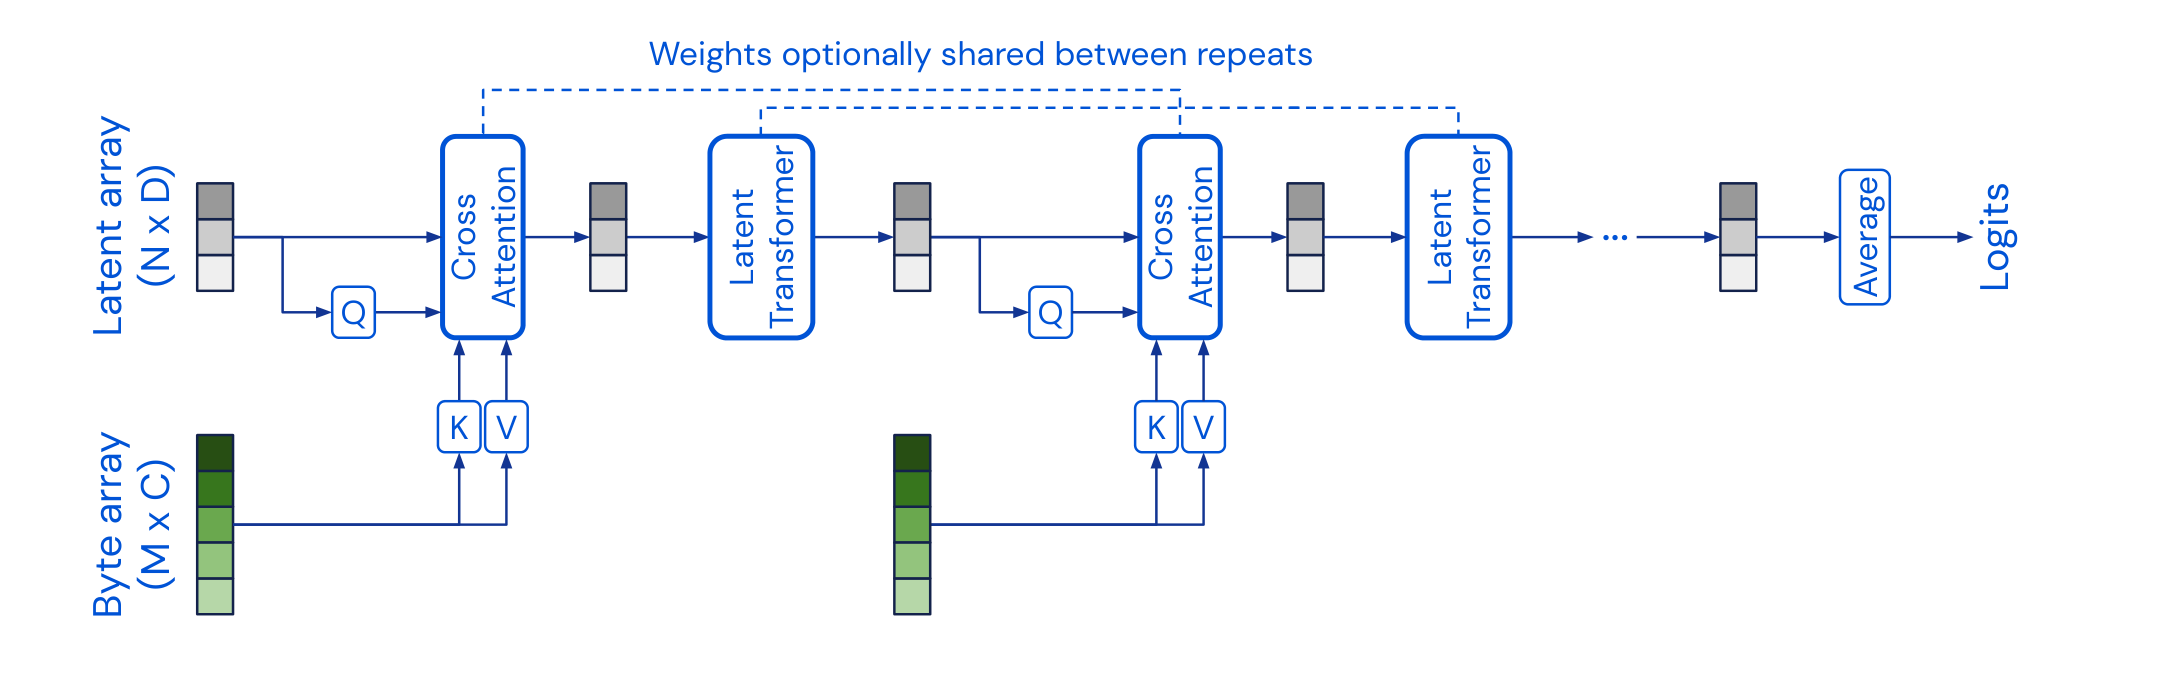
\includegraphics[width=0.97\linewidth]{./appunti_images/papers/perceiver_orig_fig1_full.png}
\caption{Il Latent Transformer nella pipeline del Perceiver originale (Jaegle et al., 2021, Fig.~1): si alterna alla cross-attention e opera \emph{solo} sui latenti $\widehat{L}\in\mathbb{R}^{N\times D}$ tramite self-attention.}
\label{fig:latent-transformer-papers}
\end{figure}

\begin{figure}[h!]
\centering
\begin{tikzpicture}[
  x=1cm, y=1cm,
  box/.style={rectangle, rounded corners=3pt, draw=blue!55, fill=blue!6,
              minimum width=5.5cm, minimum height=0.75cm, align=center, font=\small},
  iobox/.style={rectangle, rounded corners=3pt, draw=gray!60, fill=gray!12,
                minimum width=6cm, minimum height=0.8cm, align=center, font=\small\bfseries},
  plus/.style={circle, draw=blue!55, fill=white, minimum size=0.5cm, inner sep=0pt, font=\small},
  arrow/.style={->, thick},
  resarrow/.style={->, thick, blue!55, dashed}
]
% nodi
\node[iobox] (in)  at (0, 0)    {Input: $\widehat L \in \mathbb{R}^{512 \times 1024}$};
\node[box]   (ln1) at (0, -1.2) {LayerNorm};
\node[box]   (sa)  at (0, -2.3) {Multi-Head Self-Attention \quad ($H{=}8$, $d_{\text{head}}{=}128$)};
\node[plus]  (p1)  at (0, -3.4) {$+$};
\node[box]   (ln2) at (0, -4.5) {LayerNorm};
\node[box]   (mlp) at (0, -5.6) {MLP \quad $1024 \rightarrow 4096 \xrightarrow{\text{GELU}} 1024$};
\node[plus]  (p2)  at (0, -6.7) {$+$};
\node[iobox] (out) at (0, -7.8) {Output: $\widehat L^{\,(\text{next})} \in \mathbb{R}^{512 \times 1024}$};

% frecce dritte
\draw[arrow] (in) -- (ln1);
\draw[arrow] (ln1) -- (sa);
\draw[arrow] (sa) -- (p1);
\draw[arrow] (p1) -- (ln2);
\draw[arrow] (ln2) -- (mlp);
\draw[arrow] (mlp) -- (p2);
\draw[arrow] (p2) -- (out);

% residual
\draw[resarrow] (in.west)  -- ++(-2,0) |- (p1.west);
\draw[resarrow] (p1.east)  -- ++(2,0)  |- (p2.east);

% ripetizione
\node[font=\small\itshape, align=left, text=blue!70] at (5.5, -3.9) {ripetuto\\ $B = 6$\\ volte\\ (ImageNet)};
\end{tikzpicture}
\caption{Struttura interna di un blocco di Latent Transformer (pre-norm, architettura GPT-2). Opera \emph{solo} sui latenti --- forma invariata $N\times D = 512\times 1024$ --- con self-attention multi-head ($H=8$ teste da $d_{\text{head}}=128$) seguita da una MLP a hidden $4D$. Le frecce tratteggiate sono le residual connections. Il blocco è ripetuto $B=6$ volte tra due iterazioni di cross-attention.}
\label{fig:latent-transformer-block}
\end{figure}

\begin{notabox}[title={\textbf{Architettura GPT-2 nel latent transformer}}]
Il latent transformer del Perceiver non è un Transformer ``generico'': il paper (\S3.1) adotta esplicitamente l'\textbf{architettura GPT-2} (Radford et al., 2019), che a sua volta è il \emph{decoder-only} del Transformer originale (Vaswani et al., 2017) senza cross-attention sull'encoder. In pratica: LayerNorm pre-self-attention, self-attention multi-head, residual, LayerNorm pre-MLP, MLP con GELU, residual. Niente encoder, niente masking causale (il Perceiver è non-causale su tutti i blocchi).

Dimensioni per ImageNet: $H_{\text{self}} = 8$ teste, $d_{\text{head}} = D/H_{\text{self}} = 128$, MLP hidden dim $= 4D = 4096$ (standard GPT-2).
\end{notabox}

\textbf{Input}

\[\widehat{L} \in \mathbb{R}^{512 \times 1024}\]

(latenti usciti dal Cross Attention Block).

\paragraph{1. \textbf{Layer Normalization (pre-self-attention)}}

\[{\widetilde{L}}_{ij} = \gamma_{j} \cdot \frac{{\widehat{L}}_{ij} - \mu_{i}}{\sigma_{i} + \epsilon} + \beta_{j}\ ,\ \widetilde{L} \in \mathbb{R}^{512 \times 1024}\]

\begin{itemize}
\item
  Normalizziamo ogni latente.
\item
  Dimensione invariata.
\end{itemize}

La normalizzazione viene rieseguita perché prima di ogni blocco di
latent e cross si normalizza in quanto il blocco di latent non si fida
del cross attention

\paragraph{2. \textbf{Calcolo di Q,K,V (provenienti dai latenti)}}

Ora andranno ricalcolati Q, K, V, ma essendo ora in un blocco di Latent
Transformer, ci comporteremo come nel caso della self-attention dove
come input abbiamo \(\widetilde{L}\), quindi avremo:

\[\begin{matrix}
Q = \widetilde{L}W_{q}, & W_{q} \in \mathbb{R}^{1024 \times d_k}, & Q \in \mathbb{R}^{512 \times d_k} \\
K = \widetilde{L}W_{k}, & W_{k} \in \mathbb{R}^{1024 \times d_k}, & K \in \mathbb{R}^{512 \times d_k} \\
V = \widetilde{L}W_{v}, & W_{v} \in \mathbb{R}^{1024 \times d_v}, & V \in \mathbb{R}^{512 \times d_v}
\end{matrix}\]

Con $H=8$ teste e $D=1024$: $d_k = d_v = D/H = 1024/8 = 128$.

\paragraph{3. \textbf{Self-Attention sui latenti}}

Dopo aver calcolato \(Q,K,V\) :

\[\begin{matrix}
A = Softmax\left( \frac{QK^{T}}{\sqrt{d_k}} \right),\ A \in \mathbb{R}^{512 \times 512} \\
Z = AV,\ Z \in \mathbb{R}^{512 \times d_v}
\end{matrix}\]

\paragraph{4. \textbf{Proiezione + Residual (post-attention)}}

\[\begin{matrix}
Z' & \  = ZW_{O}, & \ \ \ \ \ \ \ \  & W_{O} & \  \in \mathbb{R}^{d_v \times D} \\
L' & \  = \widehat{L} + Z', & \ \ \ \ \ \ \ \  & L' & \  \in \mathbb{R}^{512 \times 1024}
\end{matrix}\]

\paragraph{5. \textbf{Feed-Forward MLP}}

\textbf{Pre-Norm:}

\[{\widetilde{L}}' = \text{ LayerNorm}\left( L' \right)\]

\textbf{Espansione:}

\[H = {\widetilde{L}}'W_{1} + b_{1},\ W_{1} \in \mathbb{R}^{1024 \times 4096},\ H \in \mathbb{R}^{512 \times 4096}\]

\textbf{Attivazione non lineare:}

\[H' = \sigma(H)\ (GELU)\]

\textbf{Compressione}:

\[F = H'W_{2} + b_{2},\ W_{2} \in \mathbb{R}^{4096 \times 1024},\ F \in \mathbb{R}^{512 \times 1024}\]

\textbf{Residual finale}

\[L^{''} = L' + F,\ L^{''} \in \mathbb{R}^{512 \times 1024}\]

\textbf{Output del blocco}

\[L^{\text{out}} = L^{''} \in \mathbb{R}^{512 \times 1024}\]

\begin{notabox}[title={\textbf{Checkpoint dimensioni --- fine \S1.4.10 (una iterazione completa)}}]
Abbiamo ora completato \emph{una} passata $T=1$ del blocco Cross-Attention $+$ MLP $+$ Latent Transformer. Dimensioni:

\medskip
\begin{center}
\begin{tabular}{@{}llll@{}}
\toprule
\textbf{Oggetto} & \textbf{Forma simbolica} & \textbf{ImageNet} & \textbf{Status} \\
\midrule
Byte array $X$ & $M \times C_{\text{tot}}$ & $50\,176 \times 261$ & input, immutato \\
Latente post cross-att $+$ MLP & $N \times D$ & $512 \times 1024$ & post blocco 1 (cross) \\
\textbf{Latente post latent transf.} & $\boldsymbol{N \times D}$ & $\mathbf{512 \times 1024}$ & output di una iterazione completa \\
\bottomrule
\end{tabular}
\end{center}

\medskip
\textbf{Invarianza dimensionale.} Cross-attention e Latent Transformer preservano entrambi la forma $512 \times 1024$ (``è la stessa matrice, solo aggiornata''): è ciò che permette di ripetere il blocco $T$ volte senza problemi di compatibilità.

\medskip
\textbf{Cosa cambia nel Latent Transformer rispetto alla cross-attention.}
\begin{itemize}\setlength\itemsep{0.1em}
\item Q, K, V provengono \emph{tutti} dai latenti ($512 \times 1024$), non dall'input.
\item $d_{QKV}$ non è più $\min(D, C_{\text{tot}}) = 261$; qui $\min(D, D) = D = 1024$, quindi si lavora in $1024$.
\item Multi-head effettivo: $H = 8$, $d_{\text{head}} = 1024/8 = 128$ (in linea con GPT-2).
\item Matrice di attenzione $A \in \mathbb{R}^{512 \times 512}$ (quadrata, non rettangolare), costo $O(N^2) = O(512^2)$: piccolo grazie al bottleneck.
\end{itemize}

\medskip
\textbf{Prossimo step} (\S\ref{sec:weight-sharing}): le $T = 8$ iterazioni con weight sharing.
\end{notabox}

\needspace{3\baselineskip}
\subsubsection{Weight Sharing e Iterazioni}
\label{sec:weight-sharing}

\pipeline{9}

Questa è una delle idee più importanti del Perceiver: dopo aver descritto \emph{un} blocco (cross-attention + latent transformer), l'intera pipeline del forward viene \textbf{riapplicata in serie $T = 8$ volte} ai medesimi latenti, \emph{condividendo i pesi} tra le iterazioni. Questa sezione spiega il funzionamento, mostra un diagramma esplicito della ricorrenza e illustra con un esempio numerico come il weight sharing si comporti nel backward pass.

\begin{figure}[h!]
\centering
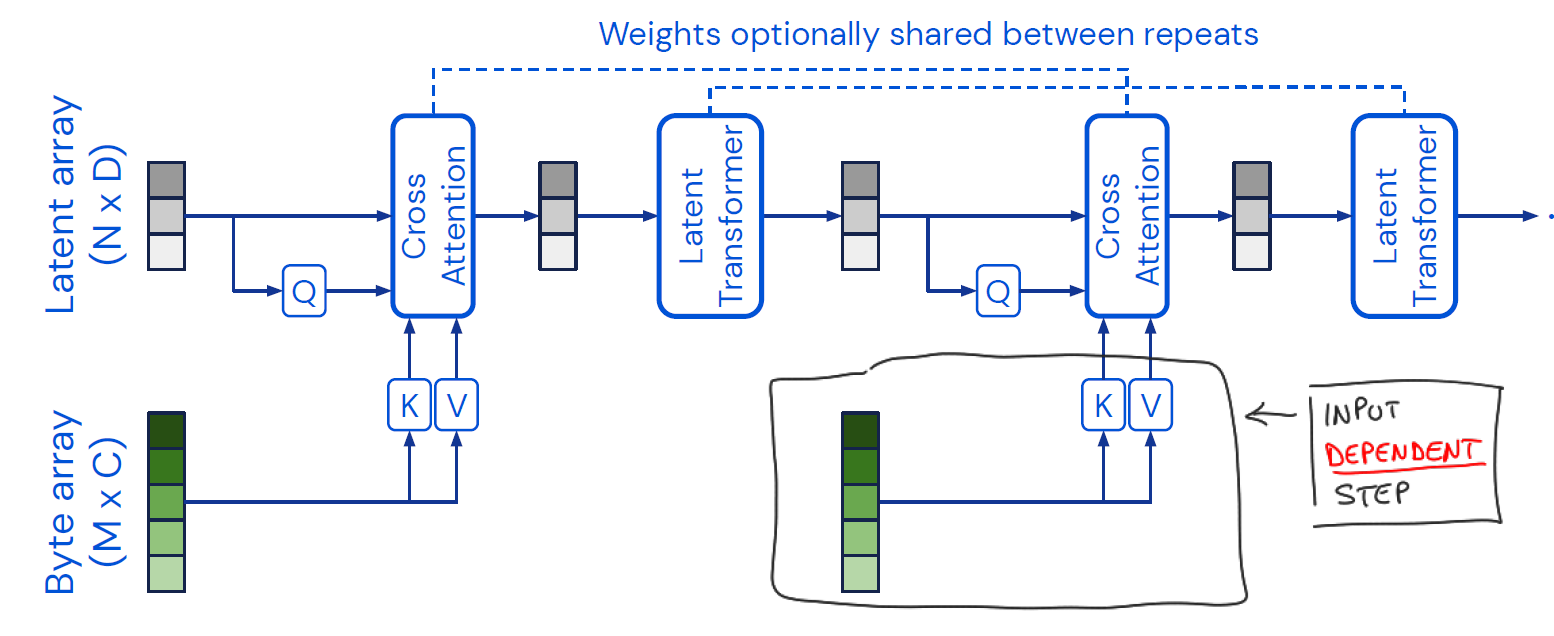
\includegraphics[width=0.85\textwidth]{./appunti_images/media/image75.png}
\caption{Architettura completa del Perceiver con weight sharing (figura dal paper Jaegle et al., 2021, Fig.\ 1). I blocchi Cross-Attention e Latent Transformer vengono ripetuti $T$ volte condividendo i pesi tra le iterazioni (linee tratteggiate).}
\end{figure}

\paragraph{Schema della ricorrenza.} Il diagramma seguente chiarisce chi condivide cosa con chi.

\begin{center}
\begin{tikzpicture}[
  >=latex,
  block/.style={draw, rounded corners=2pt, minimum width=1.1cm, minimum height=0.75cm, font=\scriptsize, align=center},
  first/.style={block, fill=orange!25, draw=orange!70!black},
  shared/.style={block, fill=seccolor!18, draw=seccolor!70!black},
  arr/.style={->, >=latex, thick, draw=gray!70},
  dot/.style={->, densely dotted, thick, draw=gray!70},
  ws/.style={dashed, thick, draw=seccolor!70!black}
]
  % Row y=0: blocchi CA e LT in sequenza
  \node[draw, rounded corners=2pt, minimum width=0.9cm, minimum height=0.7cm, font=\scriptsize, fill=gray!10] (L0)  at (-0.6, 0) {$L^{(0)}$};
  \node[first]  (CA1) at ( 0.9, 0) {$\text{CA}_1$\\\scriptsize unici};
  \node[first]  (LT1) at ( 2.2, 0) {$\text{LT}_1$\\\scriptsize unici};
  \node[shared] (CA2) at ( 3.7, 0) {$\text{CA}_2$\\\scriptsize shared};
  \node[shared] (LT2) at ( 5.0, 0) {$\text{LT}_2$\\\scriptsize shared};
  \node[shared] (CA3) at ( 6.5, 0) {$\text{CA}_3$\\\scriptsize shared};
  \node[shared] (LT3) at ( 7.8, 0) {$\text{LT}_3$\\\scriptsize shared};
  \node at ( 9.0, 0) {\scriptsize $\cdots$};
  \node[shared] (CAT) at (10.2, 0) {$\text{CA}_T$\\\scriptsize shared};
  \node[shared] (LTT) at (11.5, 0) {$\text{LT}_T$\\\scriptsize shared};
  \node[draw, rounded corners=2pt, minimum width=1.3cm, minimum height=0.75cm, font=\scriptsize, fill=gray!10] (head) at (13.1, 0) {pool+cls};

  % Frecce forward
  \draw[arr] (L0) -- (CA1); \draw[arr] (CA1) -- (LT1); \draw[arr] (LT1) -- (CA2);
  \draw[arr] (CA2) -- (LT2); \draw[arr] (LT2) -- (CA3); \draw[arr] (CA3) -- (LT3);
  \draw[arr] (LT3) -- ( 8.6, 0);
  \draw[arr] ( 9.4, 0) -- (CAT);
  \draw[arr] (CAT) -- (LTT); \draw[arr] (LTT) -- (head);

  % Weight sharing (linee tratteggiate sopra le CA e sotto le LT)
  \draw[ws] (CA2.north) to[bend left=25] (CA3.north);
  \draw[ws] (CA3.north) to[bend left=22] (CAT.north);
  \draw[ws] (LT2.south) to[bend right=25] (LT3.south);
  \draw[ws] (LT3.south) to[bend right=22] (LTT.south);

  % Byte array e frecce input
  \node[draw, rounded corners=2pt, minimum width=1.1cm, minimum height=0.55cm, font=\scriptsize, fill=gray!10] (X) at (5.0, -1.8) {byte array $X$};
  \draw[dot] (X) -- (CA1);
  \draw[dot] (X) -- (CA2);
  \draw[dot] (X) -- (CA3);
  \draw[dot] (X) -- (CAT);

  % Legenda
  \node[font=\scriptsize, anchor=west] at (-0.6, -3.0) {%
    \tikz\fill[fill=orange!25, draw=orange!70!black, rounded corners=1pt] (0,0) rectangle (0.28,0.18);\ pesi unici\quad
    \tikz\fill[fill=seccolor!18, draw=seccolor!70!black, rounded corners=1pt] (0,0) rectangle (0.28,0.18);\ pesi condivisi\quad
    \tikz\draw[ws] (0,0.08) -- (0.4,0.08);\ weight sharing\quad
    \tikz\draw[dot] (0,0.08) -- (0.4,0.08);\ lettura input
  };
\end{tikzpicture}
\end{center}

\paragraph{Regola precisa (paper, \S4.1).} I pesi sono condivisi tra tutti i blocchi \emph{tranne il primo}:
\begin{itemize}
\item \textbf{Cross-Attention}: $\text{CA}_1$ ha pesi \emph{unici}; i blocchi $\text{CA}_2, \text{CA}_3, \ldots, \text{CA}_T$ condividono tutti lo stesso set di pesi ($W_Q^{\text{sh}}, W_K^{\text{sh}}, W_V^{\text{sh}}, W_o^{\text{sh}}$).
\item \textbf{Latent Transformer}: analogamente, $\text{LT}_1$ ha pesi \emph{unici} e $\text{LT}_2, \ldots, \text{LT}_T$ condividono lo stesso blocco di $L = 6$ self-attention layer.
\end{itemize}

\textbf{Perché il primo blocco è escluso?} Il paper riporta che condividere i pesi già dal primo blocco \emph{porta a instabilità di training}. L'intuizione: la prima cross-attention è qualitativamente diversa dalle successive perché riceve i latenti nella loro inizializzazione ``neutra'' (learned position encoding $\mathcal{N}(0, 0.02^2)$), mentre dalla seconda in poi legge latenti già ``popolati'' di informazione dall'input. Due regimi così diversi non possono condividere gli stessi pesi senza causare oscillazioni del gradiente nelle prime epoche.

\paragraph{Effetto sui parametri e sulle prestazioni} (Tab.\ 7 del paper):
\begin{itemize}
\item Senza weight sharing: $\sim$326.2M parametri, $72.9\%$ validation accuracy (vs $87.7\%$ train: gap di $14.8\%$, forte overfitting).
\item Con weight sharing: $\sim$44.9M parametri, \textbf{$78.0\%$} validation accuracy (vs $79.5\%$ train: gap $1.5\%$, nessun overfitting) --- riduzione $\approx 7\times$ dei parametri e \emph{miglioramento} contemporaneo delle prestazioni.
\end{itemize}

Il weight sharing agisce dunque come regolarizzatore: le iterazioni successive sono passi di \emph{raffinamento progressivo} dei latenti, e il modello assume formalmente la struttura di un \textbf{RNN} con core ricorrente (il blocco shared $\text{CA+LT}$) applicato a uno stato ricorrente (i latenti) che legge ripetutamente lo stesso input.

\begin{notabox}[title={\textbf{Come si comporta il weight sharing nel backward pass}}]
Quando un peso $W$ viene usato in più blocchi del forward, ogni istanza del peso produce un contributo al gradiente durante il backward. Per il training corretto, questi contributi \textbf{si sommano}:
\[
\boxed{\;\frac{\partial \mathcal{L}}{\partial W^{\text{sh}}} \;=\; \sum_{t = 2}^{T}\,\frac{\partial \mathcal{L}}{\partial W^{(t)}}\;}
\]
dove $W^{(t)}$ è ``il peso come se fosse usato solo alla $t$-esima iterazione''. In PyTorch questo accade automaticamente: quando più nodi del grafo computazionale puntano allo stesso \texttt{nn.Parameter}, i gradienti calcolati in \texttt{backward()} vengono accumulati sul \texttt{.grad} del parametro --- è lo stesso meccanismo di un RNN srotolato (BPTT, \emph{back-propagation through time}).

\medskip
\textbf{Esempio numerico con $T=3$ iterazioni.} Supponiamo di avere un peso scalare condiviso $w = 2.0$ tra le iterazioni $t=2$ e $t=3$. Durante il backward si calcolano:
\[
\tfrac{\partial\mathcal{L}}{\partial w^{(2)}} = -0.3, \qquad \tfrac{\partial\mathcal{L}}{\partial w^{(3)}} = +0.1.
\]
Il gradiente effettivo che aggiorna $w$ è la \emph{somma}:
\[
\tfrac{\partial\mathcal{L}}{\partial w^{\text{sh}}} \;=\; -0.3 + 0.1 \;=\; -0.2.
\]
Con learning rate $\eta = 0.01$: $w \leftarrow w - \eta\, \tfrac{\partial\mathcal{L}}{\partial w^{\text{sh}}} = 2.0 - 0.01\cdot(-0.2) = 2.002$.

\medskip
\textbf{Attenzione:} fare l'aggiornamento \emph{due volte} (una con $-0.3$ e una con $+0.1$, come se fossero pesi distinti) produrrebbe un risultato diverso e sbagliato: l'accumulazione deve avvenire \emph{prima} del passo dell'ottimizzatore, non dopo.

\medskip
\textbf{Perché il primo blocco \emph{non} partecipa alla somma.} I pesi di $\text{CA}_1$ e $\text{LT}_1$ sono parametri separati, quindi i loro gradienti stanno in un \emph{accumulatore diverso}: non si sommano con quelli dei blocchi shared, ma vengono aggiornati in modo indipendente.
\end{notabox}

\begin{notabox}[title={\textbf{Checkpoint dimensioni --- fine \S1.4.11 (dopo $T = 8$ iterazioni)}}]
Dopo aver ripetuto il blocco $T = 8$ volte con weight sharing, i latenti sono nello stato finale. \textbf{Le dimensioni non cambiano}: ogni iterazione preserva $N \times D = 512 \times 1024$, perché è progettata per essere applicata ricorsivamente.

\medskip
\begin{center}
\begin{tabular}{@{}llll@{}}
\toprule
\textbf{Oggetto} & \textbf{Forma simbolica} & \textbf{ImageNet} & \textbf{Status} \\
\midrule
Byte array $X$ & $M \times C_{\text{tot}}$ & $50\,176 \times 261$ & riusato da ogni $\text{CA}_t$ \\
Latente iniziale $L^{(0)}$ & $N \times D$ & $512 \times 1024$ & parametro appreso \\
Latente iter.\ 1: $L^{(1)}$ & $N \times D$ & $512 \times 1024$ & post $\text{CA}_1 + \text{LT}_1$ (pesi propri) \\
Latente iter.\ 2: $L^{(2)}$ & $N \times D$ & $512 \times 1024$ & post $\text{CA}_2 + \text{LT}_2$ (pesi shared) \\
\dots & \dots & \dots & \dots \\
\textbf{Latente finale $L^{(T)}$} & $\boldsymbol{N \times D}$ & $\mathbf{512 \times 1024}$ & dopo $T=8$ iterazioni \\
\bottomrule
\end{tabular}
\end{center}

\medskip
\textbf{Osservazione chiave.} Per il paper, la struttura $L^{(t)} = \text{LT}_t(\text{CA}_t(L^{(t-1)}, X))$ con $\text{CA}_t = \text{CA}_{\text{sh}}$ e $\text{LT}_t = \text{LT}_{\text{sh}}$ per $t \geq 2$ è \emph{formalmente} un RNN con:
\begin{itemize}\setlength\itemsep{0.1em}
\item ``stato ricorrente'' = latente $L^{(t)}$ (dimensione fissa $512 \times 1024$);
\item ``input (costante nel tempo)'' = byte array $X$;
\item ``funzione di transizione'' = il blocco shared $(\text{CA}_{\text{sh}}, \text{LT}_{\text{sh}})$;
\item ``stato iniziale'' = $L^{(0)}$ (ma $L^{(1)}$ è fatto con pesi propri, quindi in realtà è un RNN con ``warm-up'' speciale al primo passo).
\end{itemize}

\medskip
Prossimo step (\S\ref{sec:output-pooling}): da $L^{(T)}$ alla classificazione finale.
\end{notabox}

\needspace{3\baselineskip}
\subsubsection{Output (Pooling + Classificazione)}
\label{sec:output-pooling}

\begin{figure}[h!]
\centering

\includegraphics[width=0.55\textwidth]{./appunti_images/media/image76.png}
\caption{Output del Perceiver: i latenti finali vengono mediati (Average + Project) e proiettati in logit per la classificazione.}
\end{figure}

\textbf{Classification Head}

\textbf{Pooling}

\begin{notabox}[title={\textbf{Pooling \emph{prima} della proiezione: un fix del paper}}]
Il Perceiver esegue l'average pooling \emph{prima} della proiezione lineare nei logit. L'Appendice F del paper chiarisce che questa è una modifica rispetto alla prima versione su arXiv: ``\emph{We have slightly improved the results ... by averaging before rather than after projecting when computing the output logits}''. Matematicamente le due operazioni (pooling e proiezione lineare) commutano se applicate a tutte le posizioni, ma fare pooling prima riduce il costo computazionale della proiezione (si applica a un solo vettore invece che a $N$) e stabilizza il training.
\end{notabox}

Il pooling è un'operazione che serve a riassumere più
vettori in uno solo. Nel caso del Perceiver, i vettori sono i latenti
finali:

\[L^{(\text{finale})} \in \mathbb{R}^{N \times D} = \mathbb{R}^{512 \times 1024}\]

dove hai \(N = 512\) latenti, ciascuno di dimensione \(D = 1024\).

Il pooling medio li combina facendo la media elemento per elemento:

\[h = \frac{1}{N}\sum_{i = 1}^{N}\, L_{i}^{(\text{finale})},\ h \in \mathbb{R}^{D} = \mathbb{R}^{1024}\]

Risultato: un unico vettore compatto che rappresenta
l'intero input.

\textbf{Perché facciamo Pooling?}

\paragraph{1. \textbf{Compressione delle informazioni}}

\begin{itemize}
\item
  Hai \(N\) latenti \(\rightarrow\) troppi per passare direttamente al
  classificatore.
\item
  Il pooling produce un solo vettore gestibile (h).
\end{itemize}

\paragraph{2. \textbf{Uniformità}}

\begin{itemize}
\item
  Indipendentemente da quanti latenti usi, dopo il pooling hai sempre un
  vettore di dimensione fissa ($D = 1024$).
\item
  Questo permette di collegarlo facilmente al classificatore lineare.
\end{itemize}

\paragraph{3. \textbf{Evita parametri aggiuntivi}}

\begin{itemize}
\item
  La media non introduce nuovi pesi.
\item
  È un metodo semplice ed efficiente per combinare i latenti.
\end{itemize}

\paragraph{4. \textbf{Analogia con altri modelli}}

\begin{itemize}
\item
  Nei Transformer (BERT, GPT), si usa un token speciale (CLS) per
  riassumere.
\item
  Nel Perceiver non c'è un token speciale: il pooling
  medio è la soluzione più diretta.
\end{itemize}

\pipeline{10}


\textbf{Classificatore Fully Connected Layer (Logits)}

Il vettore \(h\) entra in un layer lineare:

\[z = hW_{c} + b_{c}\]

\begin{itemize}
\item
  \(h \in \mathbb{R}^{1024} \rightarrow\) rappresentazione compatta
  dell'input.
\item
  \(W_{c} \in \mathbb{R}^{1024 \times 1000} \rightarrow\) matrice di pesi
  che proietta lo spazio dei latenti (1024 dimensioni) nello spazio delle
  classi (1000 per ImageNet).
\item
  \(\ b_{c} \in \mathbb{R}^{1000} \rightarrow\) vettore di bias.
\item
  \(z \in \mathbb{R}^{1000} \rightarrow\) vettore dei logit, cioè
  punteggi grezzi per ogni classe.
\end{itemize}

Concretamente: da un vettore di 1024 numeri ne ottieni uno di 1000
numeri, ognuno corrispondente a una classe.

\textbf{Perché serve questo passaggio?}

\begin{itemize}
\item
  Il pooling ti ha dato un riassunto dell'input.
\item
  Ma per decidere a quale classe appartiene, serve uno strato che
  traduce quel riassunto in punteggi di classificazione.
\item
  Il layer lineare è la funzione più semplice: una combinazione lineare
  + bias.
\end{itemize}

\begin{itemize}
\item
  Ogni colonna di \(W_{c}\) può essere vista come un "filtro" che misura
  quanto \(h\) è compatibile con una determinata classe.
\item
  Il bias \(b_{c}\) sposta il punteggio di base per ciascuna classe.
\item
  L'output \(z\) contiene i punteggi ancora non
  normalizzati.
\end{itemize}

\pipeline{11}


\textbf{Softmax sui logits}

Prendi il vettore dei logits \(z\) e applichi la funzione softmax:

\[p_{i} = \frac{e^{z_{i}}}{\sum_{j = 1}^{1000}\, e^{z_{j}}}\]

Questo trasforma i logits in probabilità normalizzate:

\begin{itemize}
\item
  Tutti i valori \(p_{i} \geq 0\).
\item
  La somma di tutte le probabilità \(= 1\).
\item
  Risultato: un vettore \(p \in \mathbb{R}^{1000}\), che rappresenta la
  probabilità di appartenenza a ciascuna classe.
\end{itemize}

\textbf{Scelta della classe predetta}

Si prende l'indice della probabilità massima:

\[\widehat{y} = \arg\max_{i}\, p_{i}\]

\(\widehat{y}\) è la classe predetta (ad esempio, "gatto" se la classe
281 corrisponde al gatto in ImageNet).

\pipeline{12}


\textbf{Loss}

La \textbf{loss} è il modo in cui ``misuri'' quanto la predizione del
modello è distante dalla verità, e serve a guidare l'aggiornamento dei
pesi durante il training.

\textbf{Esempio su ImageNet}

\begin{itemize}
\item
  Il modello produce i logits \(z \in \mathbb{R}^{1000}\).
\item
  Dopo la softmax, ottieni le probabilità predette:
\end{itemize}

\[p_{i}^{pred} = \frac{e^{z_{i}}}{\sum_{j = 1}^{1000}\, e^{z_{j}}}\]

\(con\ i = 1,\ldots,1000\).

\begin{itemize}
\item
  L'etichetta vera \(y^{true}\) (la classe corretta)
  viene rappresentata come one-hot vector:
\end{itemize}

\[y^{true} = (0,0,\ldots,1,\ldots,0)\]

dove c'è un solo 1 nella posizione della classe giusta.

\begin{itemize}
\item
  Se sei in fase di training, hai anche l'etichetta vera
  \(y\).
\item
  Usi la \hyperref[app:cross-entropy]{cross-entropy loss} (vedi Appendice~\ref{app:cross-entropy}):
\end{itemize}

\[\mathcal{L} = - \sum_{i = 1}^{K}\, y_{i}^{\text{true}}log\left( p_{i}^{pred} \right)\]

Nel nostro caso:

\[\mathcal{L} = - \sum_{i = 1}^{1000}\, y_{i}^{true}log\left( p_{i}^{pred} \right)\]

\begin{itemize}
\item
  Dove \(y_{i}\) è 1 per la classe corretta e 0 per tutte le altre
  (one-hot encoding).
\item
  Questa loss viene poi usata per aggiornare i pesi tramite
  \hyperref[app:backprop]{\textbf{backpropagation}}.
\end{itemize}

Noi vogliamo che la probabilità della classe corretta sia la più alta
possibile:

\[p_{corretta\, \rightarrow \, 1}\]

Quindi serve una funzione di \textbf{costo} che:

\begin{itemize}
\item
  sia \textbf{bassa} quando \(p_{corretta}\) è vicina a 1,
\item
  sia \textbf{alta} quando \(p_{corretta}\) è vicina a 0.
\end{itemize}

\textbf{Vediamo perché c'è il log}:

\paragraph{1. \textbf{Monotonia}}

\begin{itemize}
\item
  Il logaritmo è crescente: se \(p\) cresce, \(log(p)\) cresce.
\item
  Quindi massimizzare \(p\) equivale a massimizzare \(log(p)\).
\item
  Usiamo il -log perché stiamo minimizzando la loss (anziché
  massimizzare la probabilità).
\end{itemize}

\paragraph{2. \textbf{Penalità forte per probabilità basse}}

Se \(p_{\text{corretta}} = 0.9\) :


\[- log(0.9) \approx 0.105 \rightarrow \text{ loss bassa.}\]


Se \(p_{\text{corretta}} = 0.01\) :


\[- log(0.01) \approx 4.6 \rightarrow \text{ loss altissima.}\]


\begin{itemize}
\item
  Il log "esplode" quando \(p \rightarrow 0\), così punisce molto le
  predizioni sbagliate e sicure.
\end{itemize}

\textbf{Intuizione visiva}\\
La funzione \(- log(p)\) :

\begin{itemize}
\item
  Quando \(p = 1: - log(1) = 0 \rightarrow\) perfetta predizione.
\item
  Quando \(p \rightarrow 0: - log(p) \rightarrow + \infty \rightarrow\)
  predizione pessima.
\end{itemize}

È esattamente il comportamento che vogliamo!

\clearpage
\begin{notabox}[title={\textbf{Checkpoint dimensioni finale --- fine \S1.4 (Forward Pass completo)}}]
Ecco lo stato \emph{completo} di tutte le dimensioni al termine del forward pass per ImageNet:

\medskip
\begin{center}
{\small
\begin{tabular}{@{}llll@{}}
\toprule
\textbf{Oggetto} & \textbf{Forma simbolica} & \textbf{ImageNet} & \textbf{Cosa rappresenta} \\
\midrule
\multicolumn{4}{@{}l}{\emph{Input}} \\
Byte array grezzo & $M \times C$ & $50\,176 \times 3$ & solo RGB \\
Byte array $X$ (con Fourier PE) & $M \times C_{\text{tot}}$ & $50\,176 \times 261$ & $3$ RGB $+$ $258$ Fourier \\
\midrule
\multicolumn{4}{@{}l}{\emph{Latenti (parametro appreso)}} \\
Latente iniziale $L^{(0)}$ & $N \times D$ & $512 \times 1024$ & init $\mathcal{N}(0, 0.02^2)$ troncata \\
\midrule
\multicolumn{4}{@{}l}{\emph{Dentro una cross-attention (paper)}} \\
$W_Q$ & $D \times d_{QKV}$ & $1024 \times 261$ & proiezione dei latenti \\
$W_K$ & $C_{\text{tot}} \times d_{QKV}$ & $261 \times 261$ & proiezione input $\to$ K \\
$W_V$ & $C_{\text{tot}} \times d_{QKV}$ & $261 \times 261$ & proiezione input $\to$ V \\
$Q = L\,W_Q$ & $N \times d_{QKV}$ & $512 \times 261$ & query dai latenti \\
$K = X\,W_K$ & $M \times d_{QKV}$ & $50\,176 \times 261$ & key dall'input \\
$V = X\,W_V$ & $M \times d_{QKV}$ & $50\,176 \times 261$ & value dall'input \\
$QK^\top / \sqrt{d_{QKV}}$ & $N \times M$ & $512 \times 50\,176$ & scores rettangolari \\
$A = \text{softmax}(\cdot)$ & $N \times M$ & $512 \times 50\,176$ & pesi di attenzione \\
$F = AV$ & $N \times d_{QKV}$ & $512 \times 261$ & aggregazione (features) \\
$W_o$ & $d_{QKV} \times D$ & $261 \times 1024$ & output projection \\
$Z' = F W_o + b_o$ & $N \times D$ & $512 \times 1024$ & output proiettato \\
$L + Z'$ (post residual) & $N \times D$ & $512 \times 1024$ & latente aggiornato \\
\midrule
\multicolumn{4}{@{}l}{\emph{Dentro un latent transformer (self-attention)}} \\
$Q, K, V$ (tutti dai latenti) & $N \times D$ & $512 \times 1024$ & $H=8$, $d_{\text{head}} = D/H = 128$ \\
$A$ quadrata & $N \times N$ & $512 \times 512$ & costo $O(N^2)$ \\
$L^{(t)}$ post latent transf. & $N \times D$ & $512 \times 1024$ & \\
\midrule
\multicolumn{4}{@{}l}{\emph{Iterazione $T = 8$ volte (weight sharing dal 2° blocco in poi)}} \\
$L^{(T)}$ (latente finale) & $N \times D$ & $512 \times 1024$ & output iterazioni \\
\midrule
\multicolumn{4}{@{}l}{\emph{Output head}} \\
$h = \frac{1}{N}\sum_i L^{(T)}_i$ & $\mathbb{R}^{D}$ & $\mathbb{R}^{1024}$ & pooling \\
$W_c$ & $D \times K_{\text{cls}}$ & $1024 \times 1000$ & classificatore \\
$z = hW_c + b_c$ & $\mathbb{R}^{K_{\text{cls}}}$ & $\mathbb{R}^{1000}$ & logit (1 per classe) \\
$p = \text{softmax}(z)$ & $\mathbb{R}^{K_{\text{cls}}}$ & $\mathbb{R}^{1000}$ & probabilità \\
$\hat{y} = \arg\max_i p_i$ & scalare & $\{0, \ldots, 999\}$ & classe predetta \\
$\mathcal{L} = -\log p_{y_{\text{true}}}$ & scalare & $\mathbb{R}$ & cross-entropy loss \\
\bottomrule
\end{tabular}
}
\end{center}

\medskip
Legenda dei simboli:
\begin{itemize}\setlength\itemsep{0.1em}
\item $M$ = numero di elementi di input (pixel per ImageNet)
\item $N$ = numero di latenti
\item $C$ = canali originali dell'input, $C_{\text{tot}} = C + d(2K+1)$ dopo Fourier
\item $D$ = dimensione dei latenti (canale del latent transformer)
\item $d_{QKV}$ = dimensione interna dell'attention, $\min(D, C_{\text{tot}})$ nel paper
\item $K$ = bande di frequenza per Fourier (da non confondere con $K_{\text{cls}}$ = numero di classi)
\item $T$ = numero di iterazioni cross-att $+$ latent transformer
\item $H$ = numero di teste dell'attention, $d_{\text{head}} = D/H$
\end{itemize}

\medskip
\textbf{Due osservazioni finali:}
\begin{itemize}\setlength\itemsep{0.2em}
\item La forma $512 \times 1024$ dei latenti viene preservata da tutti i blocchi successivi alla cross-attention iniziale, fino al pooling. Questo è il ``canale'' costante su cui l'informazione viaggia.
\item L'unica compressione ``hard'' della pipeline è il pooling finale $512 \times 1024 \to \mathbb{R}^{1024}$ (un fattore $512\times$ di riduzione), seguito dalla proiezione lineare a $1000$ classi. Tutto il resto è ``trasformazione di pari dimensione'' (i blocchi latent) o ``lettura asimmetrica'' (la cross-attention $M \to N$).
\end{itemize}
\end{notabox}

\needspace{4\baselineskip}
\subsection{Backward Pass}
\label{sec:backward}

Alla fine del forward pass abbiamo la loss \(\mathcal{L}\), cioè una
misura numerica di quanto la predizione del modello (\(p\)) è lontana
dalla verità \((y)\). Questa loss però, da sola, non basta a migliorare
i pesi: per sapere come modificare i parametri della rete dobbiamo
calcolare quanto la loss dipende dai valori interni del modello (logits,
latenti, pesi, ecc.). Per fare ciò utiliziamo il gradiente.

\begin{tcolorbox}[title={\textbf{Forward \& Backward Pass --- Overview}},
  colback=white, colframe=seccolor!70, boxrule=0.6pt, arc=4pt,
  left=6pt, right=6pt, top=6pt, bottom=6pt,
  fonttitle=\small, coltitle=white, colbacktitle=seccolor!70, breakable]
{\small\textbf{Forward} ($\longrightarrow$):\par
\smallskip
Input $\to$ Embedding $\to$ Cross-Att $\to$ Res+LN $\to$ Self-Att ($\times T$) $\to$ Pooling $\to$ Classifier $\to$ Softmax $\to$ Loss}
\tcblower
{\small\textbf{Backward} ($\longleftarrow$):\par
\smallskip
Loss $\leftarrow$ Softmax $\leftarrow$ Classifier $\leftarrow$ Pooling $\leftarrow$ Latenti $\leftarrow$ Latent Transf.\ ($\times T$) $\leftarrow$ MLP $\leftarrow$ Attn $\leftarrow$ Q/K/V $\leftarrow$ LN $\leftarrow$ Cross-Att $\leftarrow$ Embedding $\leftarrow$ Input}
\end{tcolorbox}

\begin{notabox}[title={\textbf{Struttura di questa sezione e priorità di studio}}]
Il backward pass viene derivato step-by-step, risalendo dalla Loss fino all'Input. Per ogni blocco si mostra: (1) il richiamo del forward, (2) la derivata con la regola della catena, (3) le formule dei gradienti verso pesi e input. I marker \texttt{\textbackslash currentstep\{...\}} indicano la posizione attuale nel percorso.

\medskip\textbf{Per uno studio mirato all'esame}, queste sono le priorità (in ordine decrescente di importanza):
\begin{enumerate}\setlength\itemsep{0.15em}
\item \textbf{Classifier + Softmax + Cross-Entropy} (\S\ref{sec:backward}, prima parte): la combinazione softmax\,+\,CE produce il celebre gradiente $\partial\mathcal{L}/\partial z = p - y$. \emph{Essenziale, chiesto quasi sempre}.
\item \textbf{Scaled Dot-Product Attention}: backward attraverso softmax e prodotti $QK^\top$, $AV$. È il cuore geometrico dell'attention --- \emph{chiesto frequentemente}.
\item \textbf{Proiezioni lineari $Q, K, V$ e Output projection $W_o$}: applicazione diretta della chain rule a $Y = XW$. \emph{Veloce ma istruttivo}.
\item \textbf{Latent Transformer (self-attention + MLP)}: stessa logica del Cross-Attention. \emph{Saperlo riconoscere come ``stesso blocco''}.
\item \textbf{LayerNorm + Residual + Weight Sharing}: dettagli tecnici. \emph{Approfondimento, non sempre richiesto}.
\end{enumerate}

Se hai poco tempo, leggi a fondo i punti 1--3, sfoglia il resto.
\end{notabox}

\begin{notabox}[title={\textbf{Nota sul weight sharing nel backward}}]
Le formule che seguono derivano il gradiente \emph{per un singolo blocco} (una cross-attention o un latent transformer). Nel Perceiver il blocco $\text{CA+LT}$ è però applicato $T = 8$ volte con \textbf{pesi condivisi} tra le iterazioni $2, \ldots, T$ (cfr.\ \S\ref{sec:weight-sharing}). Di conseguenza, il gradiente di un peso condiviso $W^{\text{sh}}$ è la \emph{somma} dei gradienti calcolati in ogni iterazione:
\[
\frac{\partial \mathcal{L}}{\partial W^{\text{sh}}} = \sum_{t=2}^{T} \frac{\partial \mathcal{L}}{\partial W^{(t)}}
\]
In PyTorch questa somma è automatica: ogni chiamata a \texttt{backward()} accumula il gradiente sul \texttt{.grad} del parametro condiviso. I pesi del primo blocco ($\text{CA}_1$, $\text{LT}_1$), che sono unici, ricevono un solo contributo.
\end{notabox}

\begin{notabox}[title={\textbf{Nota su $b_Q$, $b_K$, $b_V$: bias nelle proiezioni Q/K/V}}]
Nel paper originale (App.\ C) e nel codice del progetto (\texttt{src/perceiver/attention.py}: \texttt{nn.Linear(..., bias=False)}) le proiezioni di Query, Key e Value nella cross-attention e nel latent self-attention \textbf{non usano bias}. Le formule che seguono includono $b_Q$, $b_K$, $b_V$ per completezza didattica --- derivare con bias è un modo pulito per praticare la chain rule --- ma nel Perceiver reale i termini $b_Q$, $b_K$, $b_V$ e i relativi gradienti $\partial \mathcal{L}/\partial b_Q$, $\partial \mathcal{L}/\partial b_K$, $\partial \mathcal{L}/\partial b_V$ \emph{non esistono}.

\medskip
I bias sono invece presenti (e le formule valgono) in:
\begin{itemize}\setlength\itemsep{0.2em}
\item \textbf{Output projection} $W_o$ della cross-attention: $Z' = Z W_o + b_o$
\item \textbf{MLP feed-forward}: $H = \tilde L W_1 + b_1$, $F = H' W_2 + b_2$
\item \textbf{Classificatore finale}: $z = h W_c + b_c$
\item \textbf{Input embedding}: $X = X_{\text{raw}} W_E + b_E$
\end{itemize}
\end{notabox}

\[\mathcal{L} = - \sum_{i = 1}^{K}\, y_{i}^{\text{true}}log\left( p_{i}^{pred} \right)\]

\textbf{1 Perché serve il gradiente?}

\begin{itemize}
\item
  L'obiettivo del training è ridurre la loss
  \(\mathcal{L}\) aggiustando i pesi della rete.
\item
  L'algoritmo che usiamo (tipicamente \textbf{discesa
  del gradiente}) aggiorna i parametri nella direzione che diminuisce la
  loss più velocemente.
\item
  Per sapere in che direzione muovere i pesi, dobbiamo sapere quanto la
  loss cambia se cambiano i valori interni della rete (logits, pesi,
  attivazioni, ecc.).
\end{itemize}

Questa \textbf{informazione ce la dà il gradiente}.

Il backward pass funziona con la \textbf{regola della catena}: se hai
una funzione composta, per aggiornare i pesi devi risalire gradualmente
dall'uscita (loss) fino ai parametri interni.

Nel nostro caso:

\[h\overset{\phantom{W_{c},b_{c}\ }}{\rightarrow}z\overset{\phantom{\text{ softmax}\ }}{\rightarrow}p\overset{\phantom{\text{ cross-entropy}\ }}{\rightarrow}\mathcal{L}\]

\begin{itemize}
\item
  Per arrivare a \(W_{c}\) e \(h\), bisogna passare per
  \(z\  \rightarrow\) Quindi il primo gradiente utile da calcolare è:
\end{itemize}


\[\frac{\partial\mathcal{L}}{\partial z}\]

Con \(z = hW_{c} + b_{c}\)


\textbf{2. Perché proprio $\frac{\partial\mathcal{L}}{\partial z}$?}


La loss $\mathcal{L}$ dipende dai logits $z$ attraverso softmax + cross-entropy.


\[\mathcal{L} = - \sum_{k = 1}^{K}\, y_{k}logp_{k}\]

dove:

\[p_{k} = \frac{e^{z_{k}}}{\sum_{j = 1}^{K}\, e^{z_{j}}}\]


Se sostituiamo \(p_{k}\) nella loss


\[\mathcal{L} = - \sum_{k = 1}^{K}\, y_{k}log\left( \frac{e^{z_{k}}}{\sum_{j = 1}^{K}\, e^{z_{j}}} \right)\]


Semplificando il logaritmo (Ricorda che
\(log\frac{a}{b} = loga - logb\))\\
Quindi:


\[\mathcal{L} = - \sum_{k = 1}^{K}\, y_{k}\left( z_{k} - log\sum_{j = 1}^{K}\, e^{z_{j}} \right)\]


Separando i due termini


\[\mathcal{L} = - \sum_{k = 1}^{K}\, y_{k}z_{k} + \sum_{k = 1}^{K}\, y_{k}log\sum_{j = 1}^{K}\, e^{z_{j}}\]

Ma siccome \(y\) è one-hot (cioè \(\sum_{k}^{}\, y_{k} = 1\)
):

\[\mathcal{L} = - \sum_{k = 1}^{K}\, y_{k}z_{k} + log\sum_{j = 1}^{K}\, e^{z_{j}}\]


Derivando rispetto a \(z_{i}\ \)calcoliamo
\(\frac{\partial\mathcal{L}}{\partial z_{i}}\).


Primo termine:


\[\frac{\partial}{\partial z_{i}}\left( - \sum_{k = 1}^{K}\, y_{k}z_{k} \right) = - y_{i}\]


Secondo termine:

\[\frac{\partial}{\partial z_{i}}\left( log\sum_{j = 1}^{K}\, e^{z_{j}} \right) = \frac{1}{\sum_{j = 1}^{K}\, e^{z_{j}}} \cdot e^{z_{i}} = \frac{e^{z_{i}}}{\sum_{j = 1}^{K}\, e^{z_{j}}} = p_{i}\]

Risultato finale

\[\frac{\partial\mathcal{L}}{\partial z_{i}} = p_{i} - y_{i}\]

oppure, in forma vettoriale:

\[\frac{\partial\mathcal{L}}{\partial z} = p - y\]

Per aggiornare
\(\mathbf{W}_{\mathbf{c}}\mathbf{,}\mathbf{b}_{\mathbf{c}}\) \textbf{e}
\(\mathbf{h}\) devo sapere quanto cambia la loss se cambiano loro.\\
Con la \textbf{regola della catena}:

\[\begin{matrix}
\frac{\partial\mathcal{L}}{\partial h} & \  = \frac{\partial\mathcal{L}}{\partial z} \cdot \frac{\partial z}{\partial h} \\
\frac{\partial\mathcal{L}}{\partial W_{c}} & \  = \frac{\partial\mathcal{L}}{\partial z} \cdot \frac{\partial z}{\partial W_{c}} \\
\frac{\partial\mathcal{L}}{\partial b_{c}} & \  = \frac{\partial\mathcal{L}}{\partial z} \cdot \frac{\partial z}{\partial b_{c}}
\end{matrix}\]

\paragraph{Gradiente rispetto a $h$}


Formula

\[\frac{\partial\mathcal{L}}{\partial h} = \frac{\partial\mathcal{L}}{\partial z} \cdot \frac{\partial z}{\partial h}\]

Dove:


\begin{itemize}
\item
  \(z = hW_{c} + b_{c}\)
\item
  La derivata di \(z\) rispetto a \(h\) è:
\end{itemize}


\[\frac{\partial z}{\partial h} = W_{c}\]


Quindi:


\[\frac{\partial\mathcal{L}}{\partial h} = (p - y)W_{c}^{\top}\]


Esplicitando indici:


\[\frac{\partial\mathcal{L}}{\partial h_{j}} = \sum_{k = 1}^{K}\,\left( p_{k} - y_{k} \right)W_{c,jk}\ \ \ \ \ j = 1,\ldots,D\]

Significato: ogni componente di \(h\) riceve un contributo da tutte le
classi, pesato dai corrispondenti elementi della matrice \(W_{c}\).


\paragraph{Gradiente rispetto a $W_c$}


Formula

\[\frac{\partial\mathcal{L}}{\partial W_{c}} = \frac{\partial\mathcal{L}}{\partial z} \cdot \frac{\partial z}{\partial W_{c}}\]

Dove:


\begin{itemize}
\item
  \(z = hW_{c} + b_{c}\).
\item
  Ogni logit è:
\end{itemize}


\[z_{k} = \sum_{j = 1}^{D}\, h_{j}W_{c,jk} + b_{c,k}\]


Derivata di \(z_{k}\) rispetto a \(W_{c,jk}\) :


\[\frac{\partial z_{k}}{\partial W_{c,jk}} = h_{j}\]


Quindi:


\[\frac{\partial\mathcal{L}}{\partial W_{c,jk}} = \left( p_{k} - y_{k} \right)h_{j}\]


Forma compatta matriciale:


\[\frac{\partial\mathcal{L}}{\partial W_{c}} = h^{\top}(p - y)\]

Significato: ogni peso \(W_{c,jk}\) viene aggiornato in base al valore
della componente \(h_{j}\) e all'errore della classe
\(k\).


\paragraph{Gradiente rispetto a $b_c$}


Formula

\[\frac{\partial\mathcal{L}}{\partial b_{c}} = \frac{\partial\mathcal{L}}{\partial z} \cdot \frac{\partial z}{\partial b_{c}}\]

Dove:


\begin{itemize}
\item
  \(z = hW_{c} + b_{c}\).
\item
  Derivata di \(z_{k}\) rispetto a \(b_{c,k}\) :
\end{itemize}


\[\frac{\partial z_{k}}{\partial b_{c,k}} = 1\]


Quindi:


\[\frac{\partial\mathcal{L}}{\partial b_{c,k}} = \left( p_{k} - y_{k} \right)\]


Forma compatta:


\[\frac{\partial\mathcal{L}}{\partial b_{c}} = p - y\]

Significato: ogni bias riceve direttamente l'errore
associato alla propria classe.


Quindi:

\textbf{Verso $h$:}

\[\frac{\partial\mathcal{L}}{\partial h} = (p - y)W_{c}^{\top}\]

$\rightarrow$ distribuisce l'errore nello spazio dei
latenti.

\textbf{Verso $W_c$:}

\[\frac{\partial\mathcal{L}}{\partial W_{c}} = h^{\top}(p - y)\]

$\rightarrow$ aggiorna la matrice dei pesi del classificatore.

\textbf{Verso $b_c$:}

\[\frac{\partial\mathcal{L}}{\partial b_{c}} = p - y\]

\(\rightarrow\) ogni bias prende l'errore della sua
classe.

\begin{notabox}[title={\textbf{Checkpoint gradienti --- fine Loss + Softmax + Classifier}}]
Partendo dalla loss, abbiamo calcolato i primi gradienti risalendo fino all'input del classifier ($h$, il vettore post-pooling). Regola chiave: \emph{ogni gradiente $\partial\mathcal{L}/\partial X$ ha la stessa forma di $X$.}

\medskip
\begin{center}
\begin{tabular}{@{}llll@{}}
\toprule
\textbf{Gradiente} & \textbf{Forma simbolica} & \textbf{ImageNet} & \textbf{Uso} \\
\midrule
$\partial\mathcal{L}/\partial z = p - y$ & $\mathbb{R}^{K_{\text{cls}}}$ & $\mathbb{R}^{1000}$ & intermedio \\
$\partial\mathcal{L}/\partial W_c = h^\top (p - y)$ & $\mathbb{R}^{D \times K_{\text{cls}}}$ & $\mathbb{R}^{1024 \times 1000}$ & \textbf{aggiorna $W_c$} \\
$\partial\mathcal{L}/\partial b_c = p - y$ & $\mathbb{R}^{K_{\text{cls}}}$ & $\mathbb{R}^{1000}$ & \textbf{aggiorna $b_c$} \\
$\partial\mathcal{L}/\partial h = (p-y) W_c^\top$ & $\mathbb{R}^{D}$ & $\mathbb{R}^{1024}$ & propaga verso latenti post-pooling \\
\bottomrule
\end{tabular}
\end{center}

\medskip
Stato: due parametri già ``pronti per l'update'' ($W_c, b_c$). L'errore è un vettore di dim $D=1024$ da ridistribuire sui $N=512$ latenti originari tramite il backward del pooling (prossimo step).
\end{notabox}

\[\ \]

\textbf{Ricordiamo cosa succede nel forward}

\begin{itemize}
\item
  Hai \(N\) latenti finali
  \(L^{\text{(finale)}} \in \mathbb{R}^{N \times D}\).
\item
  Applichi average pooling per ottenere un unico vettore compatto
  \(h \in \mathbb{R}^{D}\) :
\end{itemize}


\[h = \frac{1}{N}\sum_{i = 1}^{N}\, L_{i}\]


Quindi ogni decisione di classificazione dipende da tutti i latenti,
mediati insieme.

\textbf{Nel backward pooling}

Il backward serve a propagare l'errore (il gradiente
della loss) non solo a \(h\), ma a ciascun latente.\\
\textbf{Perché?}

\begin{itemize}
\item
  Se ci fermassimo a \(h\), sapremmo solo "quanto
  l'errore dipende dal vettore medio", ma non sapremmo
  come aggiornare i singoli latenti \(L_{i}\).
\item
  La rete, invece, ha bisogno di sapere quanto ciascun latente ha
  contribuito all'errore, per poterne correggere i
  valori attraverso i pesi che l'hanno generato.
\end{itemize}

Il backward pooling è quindi il meccanismo che distribuisce
l'errore dai logit \(\rightarrow\) al vettore medio
\(h \rightarrow\) ai latenti \(L_{i}\).\\
Sappiamo che:

\[\frac{\partial\mathcal{L}}{\partial h} \in \mathbb{R}^{D}\]

Ora, per ogni latente \(L_{i}\) :

\[h = \frac{1}{N}\sum_{i = 1}^{N}\, L_{i}\]

Quando scrivi

\[\frac{\partial h}{\partial L_{i}}\]

non stai derivando un numero rispetto a un numero, ma un vettore
rispetto a un altro vettore. Il risultato non è uno scalare, ma una
\textbf{matrice jacobiana}.

Dato che

\[h = \frac{1}{N}\left( L_{1} + L_{2} + \cdots + L_{N} \right)\]

prendiamo un singolo \(L_{i}\).

Il contributo di \(L_{i}\) a \(h\) è:

\[h = \cdots + \frac{1}{N}L_{i} + \ldots\]

cioè, semplicemente \(L_{i}\) moltiplicato per \(\frac{1}{N}\)

Se guardo una componente \(h_{j}\) :

\[h_{j} = \frac{1}{N}L_{i,j} + \text{ (altre parti)}\]

quindi:

\[\frac{\partial h_{j}}{\partial L_{i,k}} = \left\{ \begin{matrix}
\frac{1}{N} & \text{ se}j = k \\
0 & \text{ se}j \neq k
\end{matrix} \right.\ \]

Derivata di \(h\) rispetto a un singolo latente \(L_{i}\) :

\[\frac{\partial h}{\partial L_{i}} = \frac{1}{N}I_{D}\]

Dovendo propagare l'errore da \(h\) ad ogni latente \(L_{i}\),
applicando la catena:

\[\begin{matrix}
\frac{\partial\mathcal{L}}{\partial L_{i}} = \frac{\partial\mathcal{L}}{\partial h} \cdot \frac{\partial h}{\partial L_{i}} \\
\frac{\partial\mathcal{L}}{\partial L_{i}} = \frac{1}{N}\frac{\partial\mathcal{L}}{\partial h}
\end{matrix}\]

Cioè, l'errore della Loss viene ridistribuita ad ogni latente in modo
uniforme (ovvero riceve la stessa quota \(\frac{1}{N}\) del gradiente)

Facciamo la media perché i latenti, dopo molti strati di self-attention,
sono già stati ``mescolati'' e contengono informazioni simili →
trattarli uguali non è un grosso problema.

Quindi: con la media ``accusi tutti allo stesso modo''. Se vuoi dare più
colpa a chi pesa di più, devi introdurre \textbf{pooling pesato} (ad
esempio attention pooling).

\begin{notabox}[title={\textbf{Checkpoint gradienti --- fine Pooling backward}}]
Il pooling non ha parametri (è una media): non c'è nulla da aggiornare. Il suo backward è solo \emph{propagare}: l'errore su $h$ viene ridistribuito uniformemente sui $N$ latenti.

\medskip
\begin{center}
\begin{tabular}{@{}llll@{}}
\toprule
\textbf{Gradiente} & \textbf{Forma simbolica} & \textbf{ImageNet} & \textbf{Uso} \\
\midrule
$\partial\mathcal{L}/\partial h$ (da classifier) & $\mathbb{R}^{D}$ & $\mathbb{R}^{1024}$ & in ingresso al pooling \\
$\partial\mathcal{L}/\partial L_i^{(\text{finale})} = \frac{1}{N}\,\partial\mathcal{L}/\partial h$ & $\mathbb{R}^{D}$ ($\times N$) & $\mathbb{R}^{1024}$ ($\times 512$) & propaga a ogni latente \\
$\partial\mathcal{L}/\partial L^{(\text{finale})}$ (matrice completa) & $\mathbb{R}^{N \times D}$ & $\mathbb{R}^{512 \times 1024}$ & input al backward latent transformer \\
\bottomrule
\end{tabular}
\end{center}

\medskip
\textbf{Parametri pronti finora:} $W_c$, $b_c$ (del classifier). Da qui in avanti entriamo nella pipeline ``profonda'': T blocchi Cross-Attention + Latent Transformer da attraversare in reverse, ciascuno con molti parametri.
\end{notabox}

\textbf{Backward nel Latent Transformer}

\currentstep[5]{Latent Transformer}

Attualmente abbiamo fatto loss \(\rightarrow\) softmax \(\rightarrow\)
classificatore lineare \(\rightarrow\) pooling \(\rightarrow\) latenti
i-esimi

\begin{figure}[h!]
\centering

\includegraphics[width=0.55\textwidth]{./appunti_images/media/image77.png}
\caption{Schema del classification head: Latent Transformer $\to$ Average $\to$ Logits, attraverso cui risale il gradiente durante il backpropagation.}
\end{figure}

Ed
abbiamo un gradiente su ciascun latente finale:

\[\frac{\partial\mathcal{L}}{\partial L_{i}^{\text{(finale)}}} = \frac{1}{N}\frac{\partial\mathcal{L}}{\partial h} \in \mathbb{R}^{D},\quad i = 1,\ldots,N\]

Ora dobbiamo risalire dentro al Latent Transformer Module (cioè, i
blocchi self-attention + MLP).

L'ultimo step del Latent Transformer era il residual quindi faccio il
gradiente sul Residual post-MLP

\[L^{(\text{finale})} = \widetilde{L} + F\]

dove:

\begin{itemize}
\item
  \(\widetilde{L} =\) latenti normalizzati,
\item
  \(F =\) output dell'MLP.
\end{itemize}

Quindi una somma elemento per elemento.\\
Dovendo fare una derivata rispetto a una somma, la regola generale:

\[y = a + b\]

allora:

\[\frac{\partial y}{\partial a} = 1\ \ \ \ \ \ \ \ \ \ \ \ \ \ \ \ \ \ \frac{\partial y}{\partial b} = 1\]

Applicazione al caso nostro

\[L^{(\text{finale})} = \widetilde{L} + F\]

\begin{itemize}
\item
  Ogni elemento di \(L^{\text{(finale)}}\) dipende linearmente sia dal
  corrispondente elemento di \(\widetilde{L}\) che da quello di \(F\).
\item
  Non c'è nessun coefficiente moltiplicativo diverso da
  1.
\end{itemize}

Quindi:

\[\frac{\partial L^{(\text{finale})}}{\partial\widetilde{L}} = I\ \ \ \ \ \ \ \ \frac{\partial L^{(\text{finale})}}{\partial F} = I\]

dove \(I\) è la matrice identità.\\
Applicando la regola della catena:

\[\frac{\partial\mathcal{L}}{\partial\widetilde{L}} = \frac{\partial\mathcal{L}}{\partial L^{(\text{finale})}} \cdot \frac{\partial L^{(\text{finale})}}{\partial\widetilde{L}} = \frac{\partial\mathcal{L}}{\partial L^{(\text{finale})}} \cdot I = \frac{\partial\mathcal{L}}{\partial L^{(\text{finale})}}\]

stessa cosa per \(F\) :

\[\frac{\partial\mathcal{L}}{\partial F} = \frac{\partial\mathcal{L}}{\partial L^{\text{(finale)}}}\]

Risultato: il gradiente in ingresso si copia uguale nei due rami perché
la residual connection è una semplice somma

\textbf{Backward su MLP}

Nel Forward il blocco MLP era:

\paragraph{1. \textbf{Espansione}}

\[H = \widetilde{L}W_{1} + b_{1}\ \left( W_{1} \in \mathbb{R}^{1024 \times 4096},H \in \mathbb{R}^{N \times 4096} \right)\]

\paragraph{2. \textbf{Attivazione (GELU)}}

\[H' = \sigma(H)\ (\text{ stessa forma } N \times 4096)\]

\paragraph{3. \textbf{Compressione}}

\[F = H'W_{2} + b_{2}\ \left( W_{2} \in \mathbb{R}^{4096 \times 1024},F \in \mathbb{R}^{N \times 1024} \right)\]

\paragraph{4. \textbf{Residual connection}}

\[L^{(\text{finale})} = \widetilde{L} + F\]

Nel Backward Partiamo dal gradiente che arriva da

\[\frac{\partial\mathcal{L}}{\partial L^{\text{(finale)}}}
\]Come hai visto:

\[\frac{\partial\mathcal{L}}{\partial\widetilde{L}} = \frac{\partial\mathcal{L}}{\partial L^{(\text{finale})}}\ \ \ \ \ \ \ \ \ \ \ \ \ \ \ \ \ \ \ \ \ \ \ \ \ \ \frac{\partial\mathcal{L}}{\partial F} = \frac{\partial\mathcal{L}}{\partial L^{(\text{finale})}}\]

\textbf{Ora concentriamoci sul ramo} \(\mathbf{F}\)

\paragraph{1. \textbf{Compressione:}}


\[F = H'W_{2} + b_{2}\]


Gradiente rispetto a \(W_{2}\) :


\[\frac{\partial\mathcal{L}}{\partial W_{2}} = H^{'\top}\frac{\partial\mathcal{L}}{\partial F}\]


Gradiente rispetto a \(b_{2}\) :


\[\frac{\partial\mathcal{L}}{\partial b_{2}} = \sum_{i = 1}^{N}\,\frac{\partial\mathcal{L}}{\partial F_{i}}\]


Gradiente che torna su \(H'\) :


\[\frac{\partial\mathcal{L}}{\partial H'} = \frac{\partial\mathcal{L}}{\partial F}W_{2}^{\top}\]


\paragraph{2. \textbf{Attivazione:}}


\[H' = \sigma(H)\]

Qui entra in gioco la derivata della funzione di attivazione:


Se ReLU:


\[\frac{\partial H'}{\partial H} = \left\{ \begin{matrix}
1 & \text{ se}H > 0 \\
0 & \text{ se}H \leq 0
\end{matrix} \right.\ \]


\begin{itemize}
\item
  Se GELU: derivata più complessa ma stesso concetto (una maschera
  continua).
\end{itemize}


Quindi:

\[\frac{\partial\mathcal{L}}{\partial H} = \frac{\partial\mathcal{L}}{\partial H'} \odot \sigma'(H)\]

(dove \(\odot\) è prodotto elemento per elemento).


\paragraph{3. \textbf{Espansione}:}


\[H = \widetilde{L}W_{1} + b_{1}\]


Gradiente rispetto a \(W_{1}\) :


\[\frac{\partial\mathcal{L}}{\partial W_{1}} = {\widetilde{L}}^{\top}\frac{\partial\mathcal{L}}{\partial H}\]


Gradiente rispetto a \(b_{1}\) :


\[\frac{\partial\mathcal{L}}{\partial b_{1}} = \sum_{i = 1}^{N}\,\frac{\partial\mathcal{L}}{\partial H_{i}}\]


\begin{itemize}
\item
  Gradiente che torna a \(\widetilde{L}\) (prima della residual
  connection):
\end{itemize}


\[\frac{\partial\mathcal{L}}{\partial\widetilde{L}}^{(MLP)} = \frac{\partial\mathcal{L}}{\partial H}W_{1}^{\top}\]


\paragraph{4. \textbf{Riassunto "flow"}}


II gradiente segue questo percorso:

\[\frac{\partial\mathcal{L}}{\partial L^{\text{(finale)}}} \longrightarrow \frac{\partial\mathcal{L}}{\partial F} \longrightarrow \frac{\partial\mathcal{L}}{\partial H'} \longrightarrow \frac{\partial\mathcal{L}}{\partial H} \longrightarrow \frac{\partial\mathcal{L}}{\partial\widetilde{L}}\]

e in parallelo aggiorna i pesi \(W_{2},b_{2},W_{1},b_{1}\).

\begin{notabox}[title={\textbf{Attenzione: gradiente totale su $\widetilde{L}$}}]
Poiché $\widetilde{L}$ è usato \emph{sia} come input del ramo MLP \emph{sia} dalla residual post-MLP ($L^{(\text{finale})} = \widetilde{L} + F$), il gradiente \emph{totale} che arriva a $\widetilde{L}$ è la \textbf{somma dei due contributi}:
\[
\left.\frac{\partial\mathcal{L}}{\partial\widetilde{L}}\right|_{\text{tot}} = \underbrace{\frac{\partial\mathcal{L}}{\partial L^{(\text{finale})}}}_{\text{dal ramo residual}} + \underbrace{\frac{\partial\mathcal{L}}{\partial H}\, W_1^\top}_{\text{dal ramo MLP}}
\]
Questo è l'esempio canonico di ``gradient branching'' nelle architetture con skip connections.
\end{notabox}

\begin{notabox}[title={\textbf{GELU backward --- formula esplicita}}]
Per la GELU $\sigma(x) = x \cdot \Phi(x)$ (dove $\Phi$ è la CDF della gaussiana standard), la derivata è:
\[
\sigma'(x) = \Phi(x) + x \cdot \phi(x), \qquad \phi(x) = \frac{1}{\sqrt{2\pi}} e^{-x^2/2}
\]
In pratica, nei framework si usa l'approssimazione tanh di Hendrycks \& Gimpel (2016):
\[
\sigma(x) \approx 0.5 \, x \left[1 + \tanh\!\left(\sqrt{2/\pi}(x + 0.044715\, x^3)\right)\right]
\]
la cui derivata è facile da calcolare esplicitamente o via autograd.
\end{notabox}

\begin{notabox}[title={\textbf{Checkpoint gradienti --- fine MLP backward}}]
Dopo l'MLP abbiamo i gradienti sui 4 parametri del blocco MLP e il gradiente che propaga indietro verso la LayerNorm precedente. La MLP usa hidden dim $4D = 4096$.

\medskip
\begin{center}
{\small
\begin{tabular}{@{}llll@{}}
\toprule
\textbf{Gradiente} & \textbf{Forma simbolica} & \textbf{ImageNet} & \textbf{Uso} \\
\midrule
$\partial\mathcal{L}/\partial F$ & $\mathbb{R}^{N \times D}$ & $\mathbb{R}^{512 \times 1024}$ & residual copy \\
$\partial\mathcal{L}/\partial W_2 = {H'}^\top \partial\mathcal{L}/\partial F$ & $\mathbb{R}^{4D \times D}$ & $\mathbb{R}^{4096 \times 1024}$ & \textbf{aggiorna $W_2$} \\
$\partial\mathcal{L}/\partial b_2 = \sum_i \partial\mathcal{L}/\partial F_i$ & $\mathbb{R}^{D}$ & $\mathbb{R}^{1024}$ & \textbf{aggiorna $b_2$} \\
$\partial\mathcal{L}/\partial H' = \partial\mathcal{L}/\partial F \cdot W_2^\top$ & $\mathbb{R}^{N \times 4D}$ & $\mathbb{R}^{512 \times 4096}$ & intermedio \\
$\partial\mathcal{L}/\partial H = \partial\mathcal{L}/\partial H' \odot \mathrm{GELU}'(H)$ & $\mathbb{R}^{N \times 4D}$ & $\mathbb{R}^{512 \times 4096}$ & intermedio \\
$\partial\mathcal{L}/\partial W_1 = \widetilde{L}^\top \partial\mathcal{L}/\partial H$ & $\mathbb{R}^{D \times 4D}$ & $\mathbb{R}^{1024 \times 4096}$ & \textbf{aggiorna $W_1$} \\
$\partial\mathcal{L}/\partial b_1 = \sum_i \partial\mathcal{L}/\partial H_i$ & $\mathbb{R}^{4D}$ & $\mathbb{R}^{4096}$ & \textbf{aggiorna $b_1$} \\
$\partial\mathcal{L}/\partial \widetilde{L}^{(\text{MLP})}$ & $\mathbb{R}^{N \times D}$ & $\mathbb{R}^{512 \times 1024}$ & propaga verso MLP input \\
\midrule
$\left.\partial\mathcal{L}/\partial \widetilde{L}\right|_{\text{tot}}$ & $\mathbb{R}^{N \times D}$ & $\mathbb{R}^{512 \times 1024}$ & \textbf{somma} residual $+$ MLP \\
\bottomrule
\end{tabular}
}
\end{center}

\medskip
\textbf{Parametri pronti finora:} $W_c, b_c$ (classifier) + $W_1, b_1, W_2, b_2$ (MLP di questo blocco). Se il blocco è condiviso tra le $T$ iterazioni, il gradiente calcolato \emph{si accumula} con quello delle altre iterazioni (cfr.\ \S\ref{sec:weight-sharing}).
\end{notabox}


\textbf{Layer Normalization}

\currentstep[5]{Layer Normalization}

Nel forward:

\[{\widetilde{L}}_{ij} = \gamma_{j} \cdot \frac{L_{ij}' - \mu_{i}}{\sigma_{i} + \epsilon} + \beta_{j}\]

\begin{itemize}
\item
  \(\mu_{i}\) : media sulla riga \(i\)
\item
  \(\sigma_{i}\) : deviazione standard sulla riga \(i\)
\item
  \(\gamma,\beta\) : parametri appresi (gain e bias della
  normalizzazione)
\item
  Backward della LayerNorm
\end{itemize}

Per risalire da \(\frac{\partial\mathcal{L}}{\partial\bar{L}}\) a \(L'\)
:

\paragraph{1. Gradiente rispetto a $\gamma$ e $\beta$:}

\[\begin{matrix}
\frac{\partial\mathcal{L}}{\partial\gamma_{j}} = \sum_{i}^{}\,\frac{\partial\mathcal{L}}{\partial{\widetilde{L}}_{ij}} \cdot {\widehat{L}}_{ij} \\
\frac{\partial\mathcal{L}}{\partial\beta_{j}} = \sum_{i}^{}\,\frac{\partial\mathcal{L}}{\partial{\widetilde{L}}_{ij}}
\end{matrix}\]

dove
\({\widehat{L}}_{ij} = \frac{L_{ij}' - \mu_{i}}{\sigma_{i} + \epsilon}\)

2. Gradiente rispetto a \(L'\) :

Qui si usa la catena di derivate, e la formula finale è:

\[\frac{\partial\mathcal{L}}{\partial L_{ij}'} = \frac{1}{\sigma_{i} + \epsilon}\left( \frac{\partial\mathcal{L}}{\partial{\widetilde{L}}_{ij}} \cdot \gamma_{j} - \frac{1}{D}\sum_{k}^{}\,\frac{\partial\mathcal{L}}{\partial{\widetilde{L}}_{ik}} \cdot \gamma_{k} - {\widehat{L}}_{ij} \cdot \frac{1}{D}\sum_{k}^{}\,\frac{\partial\mathcal{L}}{\partial{\widetilde{L}}_{ik}} \cdot \gamma_{k} \cdot {\widehat{L}}_{ik} \right)\]

con \(D = 1024\) (la dimensione del canale). Il denominatore $\sigma_i + \epsilon$ è coerente con il forward: la chain rule preserva lo stesso fattore di normalizzazione.

\textbf{Residual Connection (post-attention o post-MLP)}

\currentstep[5]{Residual Connection}

\textbf{Forward:}

\[L' = L + Z'\]

(dove \(L\) è l'input originale e \(Z'\) è
l'output trasformato, ad esempio da self-attention o
MLP).

\textbf{Backward:}\\
Il gradiente si divide in due rami identici perché la somma è lineare:

\[\frac{\partial\mathcal{L}}{\partial L} = \frac{\partial\mathcal{L}}{\partial L'}\ \frac{\partial\mathcal{L}}{\partial Z'} = \frac{\partial\mathcal{L}}{\partial L'}\]

Interpretazione:

\begin{itemize}
\item
  Il gradiente in uscita da \(L'\) viene copiato sia sul percorso "skip"
  \((L)\) sia sul percorso trasformato \(\left( Z' \right)\).
\item
  In questo modo, la rete può imparare sia a mantenere informazione
  grezza (via skip connection), sia a modificarla (via ramo
  trasformato).
\end{itemize}

Da qui, andando ancora indietro, tocchiamo la proiezione lineare finale
dello \(Z'\) :

\[Z' = ZW_{o} + b_o\]

\textbf{Backward - Output Projection}

\currentstep[5]{Output Projection}

\textbf{Forward}

Dopo l'attenzione otteniamo:

\[Z' = ZW_{o} + b_{o}\]

\begin{itemize}
\item
  \(Z \in \mathbb{R}^{N \times d_v}\) (output dell'attention, prima della proiezione di output)
\item
  \(W_{o} \in \mathbb{R}^{d_v \times D}\) (proietta dalla dim dell'attention alla dim dei latenti, per il residual)
\item
  \(b_{o} \in \mathbb{R}^{D}\)
\item
  \(Z' \in \mathbb{R}^{N \times D}\)
\end{itemize}

\textbf{Backward}

Sappiamo che arriva il gradiente della loss rispetto
all'uscita:

\[\frac{\partial\mathcal{L}}{\partial Z'} \in \mathbb{R}^{N \times D}\]

Dobbiamo propagare questo gradiente indietro verso \(Z,W_{o}\) e
\(b_{o}\).

\paragraph{1. Gradiente rispetto a $W_o$}


Ogni riga di \(Z\) contribuisce linearmente a \(Z'\).\\
Per la derivata matriciale:

\[\frac{\partial\mathcal{L}}{\partial W_{o}} = Z^{\top}\frac{\partial\mathcal{L}}{\partial Z'}\]


\begin{itemize}
\item
  \(Z^{\top} \in \mathbb{R}^{D \times N}\)
\item
  \(\frac{\partial\mathcal{L}}{\partial Z'} \in \mathbb{R}^{N \times D}\)
\item
  Risultato:
\end{itemize}


\[\frac{\partial\mathcal{L}}{\partial W_{o}} \in \mathbb{R}^{D \times D}\]


\paragraph{2. Gradiente rispetto a $b_o$}


II bias \(b_{o}\) viene aggiunto ad ogni riga di \(Z'\).\\
La derivata è:

\[\frac{\partial\mathcal{L}}{\partial b_{o}} = \sum_{i = 1}^{N}\,\frac{\partial\mathcal{L}}{\partial Z_{i}'}\]


\begin{itemize}
\item
  Ogni
  \(\frac{\partial\mathcal{L}}{\partial Z_{i}'} \in \mathbb{R}^{D}\)
\item
  La somma su \(i = 1..N\) restituisce:
\end{itemize}


\[\frac{\partial\mathcal{L}}{\partial b_{o}} \in \mathbb{R}^{D}\]


\paragraph{3. Gradiente rispetto a $Z$}


La derivata di \(Z' = ZW_{o} + b_{o}\) rispetto a \(Z\) è semplicemente:

\[\frac{\partial Z'}{\partial Z} = W_{o}\]

Quindi:

\[\frac{\partial\mathcal{L}}{\partial Z} = \frac{\partial\mathcal{L}}{\partial Z'}W_{o}^{\top}\]


\begin{itemize}
\item
  \(\frac{\partial\mathcal{L}}{\partial Z'} \in \mathbb{R}^{N \times D}\)
\item
  \(W_{o}^{\top} \in \mathbb{R}^{D \times D}\)
\item
  Risultato:
\end{itemize}


\[\frac{\partial\mathcal{L}}{\partial Z} \in \mathbb{R}^{N \times D}\]

\textbf{Riassunto backward output projection}


Verso \(Z\) :


\[\frac{\partial\mathcal{L}}{\partial Z} = \frac{\partial\mathcal{L}}{\partial Z'}W_{o}^{\top}\  \in \mathbb{R}^{N \times D}\]


Verso \(W_{o}\) :


\[\frac{\partial\mathcal{L}}{\partial W_{o}} = Z^{\top}\frac{\partial\mathcal{L}}{\partial Z'}\  \in \mathbb{R}^{D \times D}\]


Verso \(b_{o}\) :


\[\frac{\partial\mathcal{L}}{\partial b_{o}} = \sum_{i = 1}^{N}\,\frac{\partial\mathcal{L}}{\partial Z_{i}'}\  \in \mathbb{R}^{D}\]

\begin{notabox}[title={\textbf{Checkpoint gradienti --- fine LayerNorm + Residual + Output Projection}}]
Questi tre blocchi sono concatenati (LN $\to$ residual $\to$ output projection $W_o$) e si attraversano in reverse a catena. Lo stato dei gradienti è:

\medskip
\begin{center}
{\small
\begin{tabular}{@{}llll@{}}
\toprule
\textbf{Gradiente} & \textbf{Forma simbolica} & \textbf{ImageNet} & \textbf{Uso} \\
\midrule
\multicolumn{4}{@{}l}{\emph{LayerNorm backward}} \\
$\partial\mathcal{L}/\partial \gamma$ & $\mathbb{R}^{D}$ & $\mathbb{R}^{1024}$ & \textbf{aggiorna $\gamma$} \\
$\partial\mathcal{L}/\partial \beta$ & $\mathbb{R}^{D}$ & $\mathbb{R}^{1024}$ & \textbf{aggiorna $\beta$} \\
$\partial\mathcal{L}/\partial L'$ (3 termini) & $\mathbb{R}^{N \times D}$ & $\mathbb{R}^{512 \times 1024}$ & propaga prima della LN \\
\midrule
\multicolumn{4}{@{}l}{\emph{Residual post-attention}} \\
$\partial\mathcal{L}/\partial L$, $\partial\mathcal{L}/\partial Z'$ & $\mathbb{R}^{N \times D}$ & $\mathbb{R}^{512 \times 1024}$ & entrambi $=\partial\mathcal{L}/\partial L'$ \\
\midrule
\multicolumn{4}{@{}l}{\emph{Output Projection $W_o$}} \\
$\partial\mathcal{L}/\partial W_o = Z^\top \partial\mathcal{L}/\partial Z'$ & $\mathbb{R}^{d_{QKV} \times D}$ & $\mathbb{R}^{261 \times 1024}$ & \textbf{aggiorna $W_o$} \\
$\partial\mathcal{L}/\partial b_o = \sum_i \partial\mathcal{L}/\partial Z'_i$ & $\mathbb{R}^{D}$ & $\mathbb{R}^{1024}$ & \textbf{aggiorna $b_o$} \\
$\partial\mathcal{L}/\partial Z = \partial\mathcal{L}/\partial Z' \cdot W_o^\top$ & $\mathbb{R}^{N \times d_{QKV}}$ & $\mathbb{R}^{512 \times 261}$ & \textbf{propaga verso l'attention} \\
\bottomrule
\end{tabular}
}
\end{center}

\medskip
\textbf{Parametri pronti finora:} $W_c, b_c$ (classifier), $W_1, b_1, W_2, b_2$ (MLP), $\gamma, \beta$ (LN), $W_o, b_o$ (output projection). Il gradiente di attivazione $\partial\mathcal{L}/\partial Z \in \mathbb{R}^{512 \times 261}$ è adesso pronto per entrare nel backward dell'attention vera e propria (V, A, S, Q, K).
\end{notabox}

\textbf{Backward - Scaled Dot-Product Attention}

\currentstep[5]{Scaled Dot-Product Attention}

\textbf{Forward (richiamo)}\\
L'attenzione calcola:

\[\text{ Attention}(Q,K,V) = AV\]

con

\[A = softmax\left( \frac{QK^{\top}}{\sqrt{d_{k}}} \right)\]

\begin{itemize}
\item
  \(Q \in \mathbb{R}^{N \times d_{k}}\) (queries)
\item
  \(K \in \mathbb{R}^{M \times d_{k}}\) (keys)
\item
  \(V \in \mathbb{R}^{M \times d_{v}}\) (values)
\item
  \(QK^{\top} \in \mathbb{R}^{N \times M}\) (score matrix)
\item
  \(A \in \mathbb{R}^{N \times M}\) (matrice delle attenzioni, dopo
  softmax su ogni riga)
\item
  Output:
\end{itemize}

\[Z = AV \in \mathbb{R}^{N \times d_{v}}\]

\textbf{Backward}\\
Supponiamo di ricevere in ingresso il gradiente:

\[\frac{\partial\mathcal{L}}{\partial Z} \in \mathbb{R}^{N \times d_{v}}\]

Dobbiamo risalire a \(Q,K,V\).

\paragraph{1. Gradiente verso $V$}

\[Z = AV\]

Derivata:


\[\frac{\partial\mathcal{L}}{\partial V} = A^{\top}\frac{\partial\mathcal{L}}{\partial Z}\]


\begin{itemize}
\item
  Dimensioni:

\begin{itemize}
  \item
    \(A^{\top} \in \mathbb{R}^{M \times N}\)
  \item
    \(\frac{\partial\mathcal{L}}{\partial Z} \in \mathbb{R}^{N \times d_{v}}\)
  \end{itemize}
\end{itemize}

Risultato:

\[\frac{\partial\mathcal{L}}{\partial V} \in \mathbb{R}^{M \times d_{v}}\]

\paragraph{2. Gradiente verso $A$}

\[Z = AV\  \Rightarrow \ \frac{\partial\mathcal{L}}{\partial A} = \frac{\partial\mathcal{L}}{\partial Z}V^{\top}\]

\begin{itemize}
\item
  Dimensioni:
\item
  \(\frac{\partial\mathcal{L}}{\partial Z} \in \mathbb{R}^{N \times d_{v}}\)
\item
  \(V^{\top} \in \mathbb{R}^{d_{v} \times M}\)
\item
  Risultato:
\end{itemize}

\[\frac{\partial\mathcal{L}}{\partial A} \in \mathbb{R}^{N \times M}\]

\paragraph{3. Backward attraverso Softmax}

Abbiamo:

\[A = \text{softmax}(S), \qquad S = \frac{QK^{\top}}{\sqrt{d_k}}\]

La softmax è applicata indipendentemente su ogni riga di $S$, quindi possiamo lavorare riga per riga. La jacobiana della softmax su una riga è:

\[\frac{\partial A_{ij}}{\partial S_{ik}} = A_{ij}\bigl(\delta_{jk} - A_{ik}\bigr)\]

Applicando la chain rule $\partial \mathcal{L}/\partial S_{ik} = \sum_j (\partial \mathcal{L}/\partial A_{ij})(\partial A_{ij}/\partial S_{ik})$ e semplificando con $\sum_j A_{ij} = 1$ si ottiene la \textbf{forma esplicita compatta}:

\begin{formulabox}[title={\textbf{Softmax backward --- forma vettoriale per riga}}]
\[
\frac{\partial \mathcal{L}}{\partial S_{ik}} = A_{ik}\left(\frac{\partial \mathcal{L}}{\partial A_{ik}} \;-\; \sum_{j = 1}^{M}\, A_{ij}\,\frac{\partial \mathcal{L}}{\partial A_{ij}}\right)
\]
o equivalentemente, in notazione vettoriale per la riga $i$-esima:
\[
\frac{\partial \mathcal{L}}{\partial S_i} = A_i \odot \left(\frac{\partial \mathcal{L}}{\partial A_i} \;-\; \langle A_i,\; \partial \mathcal{L}/\partial A_i \rangle \cdot \mathbf{1}\right)
\]
con $\odot$ prodotto elemento per elemento e $\langle \cdot, \cdot \rangle$ prodotto scalare.
\end{formulabox}

\textbf{Interpretazione.} Ogni $\partial\mathcal{L}/\partial S_{ik}$ è il gradiente su $A_{ik}$ ``corretto'' sottraendo la media pesata dei gradienti sulle altre entrate della stessa riga (pesata dai pesi di attenzione $A_{ij}$). Questa correzione garantisce che il gradiente su $S$ sia ortogonale al vincolo $\sum_j A_{ij} = 1$ imposto dalla softmax.

Dimensioni finali: $\partial \mathcal{L}/\partial S \in \mathbb{R}^{N \times M}$.

\paragraph{4. Gradiente verso $Q$ e $K$}


Sappiamo:

\[S = \frac{QK^{\top}}{\sqrt{d_{k}}}\]

Verso \(Q\)

\[\frac{\partial\mathcal{L}}{\partial Q} = \frac{\partial\mathcal{L}}{\partial S}K \cdot \frac{1}{\sqrt{d_{k}}}\]


\begin{itemize}
\item
  Dimensioni:
\item
  \(\frac{\partial\mathcal{L}}{\partial S} \in \mathbb{R}^{N \times M}\)
\item
  \(K \in \mathbb{R}^{M \times d_{k}}\)
\item
  Risultato:
\end{itemize}

\[\frac{\partial\mathcal{L}}{\partial Q} \in \mathbb{R}^{N \times d_{k}}\]


Verso \(K\)

\[\frac{\partial\mathcal{L}}{\partial K} = \left( \frac{\partial\mathcal{L}}{\partial S} \right)^{\top}Q \cdot \frac{1}{\sqrt{d_{k}}}\]


\begin{itemize}
\item
  Dimensioni:
\item
  \(\left( \frac{\partial\mathcal{L}}{\partial S} \right)^{\top} \in \mathbb{R}^{M \times N}\)
\item
  \(Q \in \mathbb{R}^{N \times d_{k}}\)
\item
  Risultato:
\end{itemize}


\[\frac{\partial\mathcal{L}}{\partial K} \in \mathbb{R}^{M \times d_{k}}\]


Riassunto backward scaled dot-product attention

Verso \(V\) :

\[\frac{\partial\mathcal{L}}{\partial V} = A^{\top}\frac{\partial\mathcal{L}}{\partial Z}\  \in \mathbb{R}^{M \times d_{v}}\]

Verso \(A\) :

\[\frac{\partial\mathcal{L}}{\partial A} = \frac{\partial\mathcal{L}}{\partial Z}V^{\top}\  \in \mathbb{R}^{N \times M}\]

Verso \(S\) (pre-softmax):

\[\frac{\partial\mathcal{L}}{\partial S} \in \mathbb{R}^{N \times M}\]

Verso \(Q\) :

\[\frac{\partial\mathcal{L}}{\partial Q} = \frac{\partial\mathcal{L}}{\partial S}K \cdot \frac{1}{\sqrt{d_{k}}}\  \in \mathbb{R}^{N \times d_{k}}\]

Verso \(K\) :

\[\frac{\partial\mathcal{L}}{\partial K} = \left( \frac{\partial\mathcal{L}}{\partial S} \right)^{\top}Q \cdot \frac{1}{\sqrt{d_{k}}}\  \in \mathbb{R}^{M \times d_{k}}\]

\begin{notabox}[title={\textbf{Multi-head backward: come cambia il flusso}}]
La derivazione sopra è per single-head. Nel \emph{multi-head} ($H$ teste, ciascuna di dimensione $d_{\text{head}}$), il flusso è lo stesso ma con split/merge sulle teste. Il forward multi-head è:
\[
\underbrace{Q, K, V}_{\in \mathbb{R}^{\cdot \times H d_{\text{head}}}} \;\to\; \text{split}_H \;\to\; \underbrace{Q_h, K_h, V_h}_{\in \mathbb{R}^{\cdot \times d_{\text{head}}}} \;\to\; \underbrace{Z_h = A_h V_h}_{\in \mathbb{R}^{N \times d_{\text{head}}}} \;\to\; \text{concat}_H \;\to\; Z \in \mathbb{R}^{N \times H d_{\text{head}}} \;\to\; Z' = Z W_o
\]
Nel backward, le operazioni si invertono:

\begin{enumerate}\setlength\itemsep{0.3em}
\item Dal gradiente $\partial\mathcal{L}/\partial Z \in \mathbb{R}^{N \times H d_{\text{head}}}$ (post-$W_o$), si fa lo \textbf{split} reshape $N \times H d_{\text{head}} \to H \times N \times d_{\text{head}}$: il gradiente si ripartisce sulle teste, una fetta di $d_{\text{head}}$ colonne per ciascuna.
\item Per ogni testa $h$ si esegue la derivazione single-head già vista: $\partial\mathcal{L}/\partial V_h = A_h^\top (\partial\mathcal{L}/\partial Z_h)$, $\partial\mathcal{L}/\partial A_h = (\partial\mathcal{L}/\partial Z_h) V_h^\top$, ecc.
\item I gradienti $\partial\mathcal{L}/\partial Q_h$, $\partial\mathcal{L}/\partial K_h$, $\partial\mathcal{L}/\partial V_h$ vengono ri-concatenati lungo la dimensione head per ottenere $\partial\mathcal{L}/\partial Q$, $\partial\mathcal{L}/\partial K$, $\partial\mathcal{L}/\partial V$ nella forma $\cdot \times H d_{\text{head}}$.
\item Il backward delle proiezioni lineari $W_Q, W_K, W_V$ (che erano singole matrici di forma $D \times H d_{\text{head}}$) procede come nel single-head.
\end{enumerate}

\textbf{Dettaglio importante:} nell'implementazione (e nel codice di progetto, \texttt{attention.py}), lo split e il concat sono semplici \texttt{reshape} tensoriali, quindi il backward li attraversa senza calcolo aggiuntivo --- il gradiente ``attraversa'' i reshape. Dal punto di vista matematico, il multi-head è equivalente a $H$ attenzioni separate più piccole che condividono le stesse matrici di proiezione iniziali.
\end{notabox}

\begin{notabox}[title={\textbf{Checkpoint gradienti --- fine Scaled Dot-Product backward}}]
Lo scaled dot-product è una sequenza di operazioni elementari senza parametri (matmul, scaling, softmax, matmul): il suo backward \emph{non aggiorna nessun peso}. Produce solo gradienti che si propagano a $Q$, $K$, $V$.

\medskip
\begin{center}
{\small
\begin{tabular}{@{}llll@{}}
\toprule
\textbf{Gradiente} & \textbf{Forma simbolica} & \textbf{ImageNet} & \textbf{Uso} \\
\midrule
$\partial\mathcal{L}/\partial V = A^\top\, \partial\mathcal{L}/\partial Z$ & $\mathbb{R}^{M \times d_{QKV}}$ & $\mathbb{R}^{50\,176 \times 261}$ & \textbf{propaga verso V} \\
$\partial\mathcal{L}/\partial A = \partial\mathcal{L}/\partial Z \cdot V^\top$ & $\mathbb{R}^{N \times M}$ & $\mathbb{R}^{512 \times 50\,176}$ & intermedio \\
$\partial\mathcal{L}/\partial S$ (via jacobiana softmax) & $\mathbb{R}^{N \times M}$ & $\mathbb{R}^{512 \times 50\,176}$ & intermedio \\
$\partial\mathcal{L}/\partial Q = \partial\mathcal{L}/\partial S \cdot K / \sqrt{d_{QKV}}$ & $\mathbb{R}^{N \times d_{QKV}}$ & $\mathbb{R}^{512 \times 261}$ & \textbf{propaga verso Q} \\
$\partial\mathcal{L}/\partial K = (\partial\mathcal{L}/\partial S)^\top \cdot Q / \sqrt{d_{QKV}}$ & $\mathbb{R}^{M \times d_{QKV}}$ & $\mathbb{R}^{50\,176 \times 261}$ & \textbf{propaga verso K} \\
\bottomrule
\end{tabular}
}
\end{center}

\medskip
\textbf{Parametri pronti finora:} \emph{invariato rispetto al checkpoint precedente} --- lo scaled dot-product non ha parametri propri. Gli unici update calcolati finora sono $W_c, b_c, W_1, b_1, W_2, b_2, \gamma, \beta, W_o, b_o$. Il prossimo step (proiezioni lineari Q/K/V) userà $\partial\mathcal{L}/\partial Q, \partial\mathcal{L}/\partial K, \partial\mathcal{L}/\partial V$ per calcolare i gradienti su $W_Q, W_K, W_V$ e per propagare indietro verso i latenti e verso l'input.
\end{notabox}

\textbf{Backward - Proiezioni lineari}
\(\mathbf{Q}\mathbf{,}\mathbf{K}\mathbf{,}\mathbf{V}\)

\currentstep[5]{Proiezioni lineari Q,K,V}

\textbf{Forward (richiamo)}\\
Nel Perceiver otteniamo:

\[\begin{matrix}
Q & \  = LW_{Q} + b_{Q} \\
K & \  = XW_{K} + b_{K} \\
V & \  = XW_{V} + b_{V}
\end{matrix}\]

\begin{itemize}
\item
  \(L \in \mathbb{R}^{N \times D} =\) latenti (per Q )
\item
  \(X \in \mathbb{R}^{M \times D} =\) input embedding (per
  \(\left. \ K,V \right)\)
\item
  \(W_{Q},W_{K},W_{V} \in \mathbb{R}^{D \times d_{k}}\) oppure
  \(D \times d_{v}\)
\item
  \(b_{Q},b_{K} \in \mathbb{R}^{d_{k}},\; b_{V} \in \mathbb{R}^{d_{v}}\)
\item
  \(Q \in \mathbb{R}^{N \times d_{k}},K \in \mathbb{R}^{M \times d_{k}},V \in \mathbb{R}^{M \times d_{v}}\)
\end{itemize}

\textbf{Backward}\\
Abbiamo già calcolato dai passi precedenti:

\begin{itemize}
\item
  \(\frac{\partial\mathcal{L}}{\partial Q} \in \mathbb{R}^{N \times d_{k}}\)
\item
  \(\frac{\partial\mathcal{L}}{\partial K} \in \mathbb{R}^{M \times d_{k}}\)
\item
  \(\frac{\partial\mathcal{L}}{\partial V} \in \mathbb{R}^{M \times d_{v}}\)
\end{itemize}

Ora risaliamo a \(W_{Q},W_{K},W_{V},b_{Q},b_{K},b_{V}\) e agli input
\(L,X\).

\paragraph{1. Proiezione delle Query}

\[Q = LW_{Q} + b_{Q}\]

Verso \(W_{Q}\) :

\[\frac{\partial\mathcal{L}}{\partial W_{Q}} = L^{\top}\frac{\partial\mathcal{L}}{\partial Q}\]

\begin{itemize}
\item
  Dimensioni:
\item
  \(L^{\top} \in \mathbb{R}^{D \times N}\)
\item
  \(\frac{\partial\mathcal{L}}{\partial Q} \in \mathbb{R}^{N \times d_{k}}\)
\item
  Risultato:
\end{itemize}

\[\frac{\partial\mathcal{L}}{\partial W_{Q}} \in \mathbb{R}^{D \times d_{k}}\]

Verso \(b_{Q}\) :

\[\frac{\partial\mathcal{L}}{\partial b_{Q}} = \sum_{i = 1}^{N}\,\frac{\partial\mathcal{L}}{\partial Q_{i}}\  \in \mathbb{R}^{d_{k}}\]

Verso \(L\) :

\[\frac{\partial\mathcal{L}}{\partial L} = \frac{\partial\mathcal{L}}{\partial Q}W_{Q}^{\top}\]

\begin{itemize}
\item
  Dimensioni:
\item
  \(\frac{\partial\mathcal{L}}{\partial Q} \in \mathbb{R}^{N \times d_{k}}\)
\item
  \(W_{Q}^{\top} \in \mathbb{R}^{d_{k} \times D}\)
\item
  Risultato:
\end{itemize}

\[\frac{\partial\mathcal{L}}{\partial L} \in \mathbb{R}^{N \times D}\]

\paragraph{2. Proiezione delle Key}

\[K = XW_{K} + b_{K}\]

Verso \(W_{K}\) :

\[\frac{\partial\mathcal{L}}{\partial W_{K}} = X^{\top}\frac{\partial\mathcal{L}}{\partial K}\]

\begin{itemize}
\item
  Dimensioni:
\item
  \(X^{\top} \in \mathbb{R}^{D \times M}\)
\item
  \(\frac{\partial\mathcal{L}}{\partial K} \in \mathbb{R}^{M \times d_{k}}\)
\item
  Risultato:
\end{itemize}

\[\frac{\partial\mathcal{L}}{\partial W_{K}} \in \mathbb{R}^{D \times d_{k}}\]

Verso \(b_{K}\) :

\[\frac{\partial\mathcal{L}}{\partial b_{K}} = \sum_{i = 1}^{M}\,\frac{\partial\mathcal{L}}{\partial K_{i}}\  \in \mathbb{R}^{d_{k}}\]

Verso \(X\) (dal ramo K ):

\[\left. \ \frac{\partial\mathcal{L}}{\partial X} \right|_{K} = \frac{\partial\mathcal{L}}{\partial K}W_{K}^{\top}\]

\begin{itemize}
\item
  Dimensioni:
\item
  \(\frac{\partial\mathcal{L}}{\partial K} \in \mathbb{R}^{M \times d_{k}}\)
\item
  \(W_{K}^{\top} \in \mathbb{R}^{d_{k} \times D}\)
\item
  Risultato:
\end{itemize}

\[\left. \ \frac{\partial\mathcal{L}}{\partial X} \right|_{K} \in \mathbb{R}^{M \times D}\]

\paragraph{3. Proiezione delle Value}

\[V = XW_{V} + b_{V}\]

Verso \(W_{V}\) :

\[\frac{\partial\mathcal{L}}{\partial W_{V}} = X^{\top}\frac{\partial\mathcal{L}}{\partial V}\]

\begin{itemize}
\item
  Dimensioni:
\item
  \(X^{\top} \in \mathbb{R}^{D \times M}\)
\item
  \(\frac{\partial\mathcal{L}}{\partial V} \in \mathbb{R}^{M \times d_{v}}\)
\item
  Risultato:
\end{itemize}

\[\frac{\partial\mathcal{L}}{\partial W_{V}} \in \mathbb{R}^{D \times d_{v}}\]

Verso \(b_{V}\) :

\[\frac{\partial\mathcal{L}}{\partial b_{V}} = \sum_{i = 1}^{M}\,\frac{\partial\mathcal{L}}{\partial V_{i}}\  \in \mathbb{R}^{d_{v}}\]

Verso \(X\) (dal ramo V ):

\[\left. \ \frac{\partial\mathcal{L}}{\partial X} \right|_{V} = \frac{\partial\mathcal{L}}{\partial V}W_{V}^{\top}\]

\begin{itemize}
\item
  Dimensioni:
\item
  \(\frac{\partial\mathcal{L}}{\partial V} \in \mathbb{R}^{M \times d_{v}}\)
\item
  \(W_{V}^{\top} \in \mathbb{R}^{d_{v} \times D}\)
\item
  Risultato:
\end{itemize}

\[\left. \ \frac{\partial\mathcal{L}}{\partial X} \right|_{V} \in \mathbb{R}^{M \times D}\]

\textbf{Riassunto backward proiezioni lineari}

Verso \(W_{Q}\) :

\[\frac{\partial\mathcal{L}}{\partial W_{Q}} = L^{\top}\frac{\partial\mathcal{L}}{\partial Q}\  \in \mathbb{R}^{D \times d_{k}}\]

Verso \(b_{Q}\) :

\[\frac{\partial\mathcal{L}}{\partial b_{Q}} = \sum_{i = 1}^{N}\,\frac{\partial\mathcal{L}}{\partial Q_{i}}\  \in \mathbb{R}^{d_{k}}\]

Verso \(L\) :

\[\frac{\partial\mathcal{L}}{\partial L} = \frac{\partial\mathcal{L}}{\partial Q}W_{Q}^{\top}\  \in \mathbb{R}^{N \times D}\]

Verso \(W_{K}\) :

\[\frac{\partial\mathcal{L}}{\partial W_{K}} = X^{\top}\frac{\partial\mathcal{L}}{\partial K}\  \in \mathbb{R}^{D \times d_{k}}\]

Verso \(b_{K}\) :

\[\frac{\partial\mathcal{L}}{\partial b_{K}} = \sum_{i = 1}^{M}\,\frac{\partial\mathcal{L}}{\partial K_{i}}\  \in \mathbb{R}^{d_{k}}\]

Verso \(X\) dal ramo K :

\[\left. \ \frac{\partial\mathcal{L}}{\partial X} \right|_{K} = \frac{\partial\mathcal{L}}{\partial K}W_{K}^{\top}\  \in \mathbb{R}^{M \times D}\]

Verso \(W_{V}\) :

\[\frac{\partial\mathcal{L}}{\partial W_{V}} = X^{\top}\frac{\partial\mathcal{L}}{\partial V}\  \in \mathbb{R}^{D \times d_{v}}\]

Verso \(b_{V}\) :

\[\frac{\partial\mathcal{L}}{\partial b_{V}} = \sum_{i = 1}^{M}\,\frac{\partial\mathcal{L}}{\partial V_{i}}\  \in \mathbb{R}^{d_{v}}\]

Verso \(X\) dal ramo V :

\[\left. \ \frac{\partial\mathcal{L}}{\partial X} \right|_{V} = \frac{\partial\mathcal{L}}{\partial V}W_{V}^{\top}\  \in \mathbb{R}^{M \times D}\]

Nota importante:

Il gradiente totale su \(X\) è la somma dei contributi che arrivano dal
ramo \(K\) e dal ramo \(V\) :

\[\frac{\partial\mathcal{L}}{\partial X} = \left. \ \frac{\partial\mathcal{L}}{\partial X} \right|_{K} + \left. \ \frac{\partial\mathcal{L}}{\partial X} \right|_{V}\]

\begin{notabox}[title={\textbf{Checkpoint gradienti --- fine proiezioni lineari Q/K/V backward}}]
Questo è il backward delle tre proiezioni lineari che generano Q, K, V dai latenti ($L$) e dall'input embedded ($X$). Calcola gli update sui tre pesi $W_Q, W_K, W_V$ e propaga indietro verso $L$ (dalla Q) e verso $X$ (dalla K e dalla V).

\medskip
\begin{center}
{\small
\begin{tabular}{@{}llll@{}}
\toprule
\textbf{Gradiente} & \textbf{Forma simbolica} & \textbf{ImageNet} & \textbf{Uso} \\
\midrule
\multicolumn{4}{@{}l}{\emph{Proiezione Q (dai latenti)}} \\
$\partial\mathcal{L}/\partial W_Q = L^\top \partial\mathcal{L}/\partial Q$ & $\mathbb{R}^{D \times d_{QKV}}$ & $\mathbb{R}^{1024 \times 261}$ & \textbf{aggiorna $W_Q$} \\
$\partial\mathcal{L}/\partial L = \partial\mathcal{L}/\partial Q \cdot W_Q^\top$ & $\mathbb{R}^{N \times D}$ & $\mathbb{R}^{512 \times 1024}$ & propaga verso latenti \\
\midrule
\multicolumn{4}{@{}l}{\emph{Proiezione K (dall'input)}} \\
$\partial\mathcal{L}/\partial W_K = X^\top \partial\mathcal{L}/\partial K$ & $\mathbb{R}^{C_{\text{tot}} \times d_{QKV}}$ & $\mathbb{R}^{261 \times 261}$ & \textbf{aggiorna $W_K$} \\
$\partial\mathcal{L}/\partial X\big|_K = \partial\mathcal{L}/\partial K \cdot W_K^\top$ & $\mathbb{R}^{M \times C_{\text{tot}}}$ & $\mathbb{R}^{50\,176 \times 261}$ & contributo K \\
\midrule
\multicolumn{4}{@{}l}{\emph{Proiezione V (dall'input)}} \\
$\partial\mathcal{L}/\partial W_V = X^\top \partial\mathcal{L}/\partial V$ & $\mathbb{R}^{C_{\text{tot}} \times d_{QKV}}$ & $\mathbb{R}^{261 \times 261}$ & \textbf{aggiorna $W_V$} \\
$\partial\mathcal{L}/\partial X\big|_V = \partial\mathcal{L}/\partial V \cdot W_V^\top$ & $\mathbb{R}^{M \times C_{\text{tot}}}$ & $\mathbb{R}^{50\,176 \times 261}$ & contributo V \\
\midrule
\multicolumn{4}{@{}l}{\emph{Merge contributi verso $X$}} \\
$\partial\mathcal{L}/\partial X = \partial\mathcal{L}/\partial X\big|_K + \partial\mathcal{L}/\partial X\big|_V$ & $\mathbb{R}^{M \times C_{\text{tot}}}$ & $\mathbb{R}^{50\,176 \times 261}$ & \textbf{propaga verso input embedding} \\
\bottomrule
\end{tabular}
}
\end{center}

\medskip
\textbf{Parametri pronti finora} (fine di \emph{un} blocco cross-attention completo, dalla loss all'input embedding): $W_c, b_c$ (classifier), $W_1, b_1, W_2, b_2$ (MLP), $\gamma, \beta$ (LN), $W_o, b_o$ (output proj), $W_Q, W_K, W_V$ (proiezioni Q/K/V). I gradienti di attivazione che propagano oltre sono $\partial\mathcal{L}/\partial L$ (verso i latenti del blocco precedente, se $T > 1$) e $\partial\mathcal{L}/\partial X$ (verso l'input embedding).

\medskip
\textbf{Nota su weight sharing}: se $W_Q, W_K, W_V$ sono condivisi tra le $T$ iterazioni (cfr.\ \S\ref{sec:weight-sharing}), i gradienti sopra si \emph{accumulano} su ciascun parametro, sommando i contributi da ogni iterazione.
\end{notabox}

\paragraph{Backward - Layer Normalization (su Q/K/V)}
Forward (richiamo)\\
Dato un input \(H \in \mathbb{R}^{N \times D}\) (dove ogni riga ha
dimensione \(D\) ), la LayerNorm calcola:

\[{\widetilde{H}}_{ij} = \gamma_{j} \cdot {\widehat{H}}_{ij} + \beta_{j}\]

dove:

\begin{itemize}
\item
  \({\widehat{H}}_{ij} = \frac{H_{ij} - \mu_{i}}{\sigma_{i} + \epsilon}\)
\item
  \(\mu_{i} = \frac{1}{D}\sum_{j = 1}^{D}\, H_{ij}\) (media
  della riga \(\left. \ i \right)\)
\item
  \(\sigma_{i} = \sqrt{\frac{1}{D}\sum_{j = 1}^{D}\,\left( H_{ij} - \mu_{i} \right)^{2}}\)
  (deviazione standard della riga \(i\) )
\item
  \(\gamma,\beta \in \mathbb{R}^{D}\) (parametri appresi: gain e bias)
\item
  Output: \(\widetilde{H} \in \mathbb{R}^{N \times D}\)
\end{itemize}

Backward\\
Arriva in ingresso:

\[\frac{\partial\mathcal{L}}{\partial\widetilde{H}} \in \mathbb{R}^{N \times D}\]

Dobbiamo risalire a \(\gamma,\beta,H\).

\paragraph{1. Gradiente rispetto a $\gamma$ e $\beta$}

Verso \(\gamma\) :

\[\frac{\partial\mathcal{L}}{\partial\gamma_{j}} = \sum_{i = 1}^{N}\,\frac{\partial\mathcal{L}}{\partial{\widetilde{H}}_{ij}} \cdot {\widehat{H}}_{ij}\  \in \mathbb{R}^{D}\]

Verso \(\beta\) :

\[\frac{\partial\mathcal{L}}{\partial\beta_{j}} = \sum_{i = 1}^{N}\,\frac{\partial\mathcal{L}}{\partial{\widetilde{H}}_{ij}}\  \in \mathbb{R}^{D}\]

\begin{enumerate}
\def\labelenumi{\arabic{enumi}.}
\setcounter{enumi}{1}
\item
  Gradiente rispetto all'input normalizzato
  \(\widehat{H}\)
\end{enumerate}

Poiché:

\[{\widetilde{H}}_{ij} = \gamma_{j}{\widehat{H}}_{ij} + \beta_{j}\]

si ha:

\[\frac{\partial\mathcal{L}}{\partial{\widehat{H}}_{ij}} = \frac{\partial\mathcal{L}}{\partial{\widetilde{H}}_{ij}} \cdot \gamma_{j}\]

Forma compatta:

\[\frac{\partial\mathcal{L}}{\partial\widehat{H}} = \frac{\partial\mathcal{L}}{\partial\widetilde{H}} \odot \gamma\  \in \mathbb{R}^{N \times D}\]

\paragraph{3. Gradiente rispetto a $H$}

Ora dobbiamo tornare da \(\widehat{H}\) a \(H\).

Ricordiamo:

\[{\widehat{H}}_{ij} = \frac{H_{ij} - \mu_{i}}{\sigma_{i} + \epsilon}\]

Il gradiente finale per ogni riga \(i\) (dimensione \(D\) ) è:

\[\frac{\partial\mathcal{L}}{\partial H_{ij}} = \frac{1}{\sigma_{i} + \epsilon}\left( \frac{\partial\mathcal{L}}{\partial{\widehat{H}}_{ij}} - \frac{1}{D}\sum_{k = 1}^{D}\,\frac{\partial\mathcal{L}}{\partial{\widehat{H}}_{ik}} - {\widehat{H}}_{ij} \cdot \frac{1}{D}\sum_{k = 1}^{D}\,\frac{\partial\mathcal{L}}{\partial{\widehat{H}}_{ik}}{\widehat{H}}_{ik} \right)\]

\begin{itemize}
\item
  Dimensioni:
\item
  \(\frac{\partial\mathcal{L}}{\partial\widehat{H}} \in \mathbb{R}^{N \times D}\)
\item
  Risultato:
\end{itemize}

\[\frac{\partial\mathcal{L}}{\partial H} \in \mathbb{R}^{N \times D}\]

Riassunto backward LayerNorm

Verso \(\gamma\) :

\[\frac{\partial\mathcal{L}}{\partial\gamma_{j}} = \sum_{i = 1}^{N}\,\frac{\partial\mathcal{L}}{\partial{\widetilde{H}}_{ij}} \cdot {\widehat{H}}_{ij}\  \in \mathbb{R}^{D}\]

Verso \(\beta\) :

\[\frac{\partial\mathcal{L}}{\partial\beta_{j}} = \sum_{i = 1}^{N}\,\frac{\partial\mathcal{L}}{\partial{\widetilde{H}}_{ij}}\  \in \mathbb{R}^{D}\]

Verso \(H\) :

\[\frac{\partial\mathcal{L}}{\partial H_{ij}} = \frac{1}{\sigma_{i} + \epsilon}\left( \frac{\partial\mathcal{L}}{\partial{\widehat{H}}_{ij}} - \frac{1}{D}\sum_{k = 1}^{D}\,\frac{\partial\mathcal{L}}{\partial{\widehat{H}}_{ik}} - {\widehat{H}}_{ij} \cdot \frac{1}{D}\sum_{k = 1}^{D}\,\frac{\partial\mathcal{L}}{\partial{\widehat{H}}_{ik}}{\widehat{H}}_{ik} \right) \in \mathbb{R}^{N \times D}\]

\textbf{Backward -- Cross Attention}

\textbf{Forward (richiamo)}

\[Z = Attention(Q,K,V)W_{o} + b_{o}\]

con:

\begin{itemize}
\item
  \(Q = LW_{Q} + b_{Q} \in \mathbb{R}^{N \times d_{k}}\)
\item
  \(K = XW_{K} + b_{K} \in \mathbb{R}^{M \times d_{k}}\)
\item
  \(V = XW_{V} + b_{V} \in \mathbb{R}^{M \times d_{v}}\)
\item
  \(Z \in \mathbb{R}^{N \times d_{v}}\)
\end{itemize}

\textbf{Backward - Flusso dei gradienti}

\paragraph{1. Output projection}

Già fatto:

\[\frac{\partial\mathcal{L}}{\partial Z},\ \frac{\partial\mathcal{L}}{\partial W_{o}},\ \frac{\partial\mathcal{L}}{\partial b_{o}}\]

\paragraph{2. Scaled Dot-Product Attention}

\[\frac{\partial\mathcal{L}}{\partial V} = A^{\top}\frac{\partial\mathcal{L}}{\partial Z},\ \frac{\partial\mathcal{L}}{\partial Q} = \frac{\partial\mathcal{L}}{\partial S}K/\sqrt{d_{k}},\ \frac{\partial\mathcal{L}}{\partial K} = \left( \frac{\partial\mathcal{L}}{\partial S} \right)^{\top}Q/\sqrt{d_{k}}\]

\paragraph{3. Proiezioni lineari}

\[\begin{matrix}
\frac{\partial\mathcal{L}}{\partial W_{Q}} = L^{\top}\frac{\partial\mathcal{L}}{\partial Q}, & \frac{\partial\mathcal{L}}{\partial b_{Q}} = \sum_{i}^{}\,\frac{\partial\mathcal{L}}{\partial Q_{i}}, & \frac{\partial\mathcal{L}}{\partial L} = \frac{\partial\mathcal{L}}{\partial Q}W_{Q}^{\top} \\
\frac{\partial\mathcal{L}}{\partial W_{K}} = X^{\top}\frac{\partial\mathcal{L}}{\partial K}, & \frac{\partial\mathcal{L}}{\partial b_{K}} = \sum_{i}^{}\,\frac{\partial\mathcal{L}}{\partial K_{i}}, & \left. \ \frac{\partial\mathcal{L}}{\partial X} \right|_{K} = \frac{\partial\mathcal{L}}{\partial K}W_{K}^{\top} \\
\frac{\partial\mathcal{L}}{\partial W_{V}} = X^{\top}\frac{\partial\mathcal{L}}{\partial V}, & \frac{\partial\mathcal{L}}{\partial b_{V}} = \sum_{i}^{}\,\frac{\partial\mathcal{L}}{\partial V_{i}}, & \left. \ \frac{\partial\mathcal{L}}{\partial X} \right|_{V} = \frac{\partial\mathcal{L}}{\partial V}W_{V}^{\top}
\end{matrix}\]

\textbf{Riassunto Cross-Attention Backward}

\begin{itemize}
\item
  Il gradiente si propaga da \(Z \rightarrow\) attenzione
  \(\rightarrow\) proiezioni lineari.
\item
  Verso latenti \(L\) :
\end{itemize}

\[\frac{\partial\mathcal{L}}{\partial L} = \frac{\partial\mathcal{L}}{\partial Q}W_{Q}^{\top}\]

Verso input \(X\) :

\[\frac{\partial\mathcal{L}}{\partial X} = \left. \ \frac{\partial\mathcal{L}}{\partial X} \right|_{K} + \left. \ \frac{\partial\mathcal{L}}{\partial X} \right|_{V}\]

\begin{itemize}
\item
  Verso pesi \(W_{Q},W_{K},W_{V}\) e bias relativi: aggiornati con outer
  product tra input e gradienti.
\end{itemize}

\paragraph{Backward - Input Embedding}
Forward (richiamo)\\
All'inizio il Perceiver prende l'input
\(X_{\text{raw}}\) (es. immagine, audio, testo) e lo passa in un
embedding lineare o una piccola convoluzione per portarlo nello spazio
latente \(D\) :

\[X = X_{\text{raw}}W_{E} + b_{E}\]

\begin{itemize}
\item
  \(X_{\text{raw}} \in \mathbb{R}^{M \times C}\) ( \(M =\) numero
  token/pixel/patch, \(C =\) canali originali )
\item
  \(W_{E} \in \mathbb{R}^{C \times D}\) (matrice embedding)
\item
  \(b_{E} \in \mathbb{R}^{D}\) (bias embedding)
\item
  \(X \in \mathbb{R}^{M \times D}\) (embedding usato per \(K,V\) )
\end{itemize}

Backward\\
Dopo aver fatto il backward della cross-attention, abbiamo già ottenuto:

\[\frac{\partial\mathcal{L}}{\partial X} \in \mathbb{R}^{M \times D}\]

Ora risaliamo.

Verso \(W_{E}\) :

\[\frac{\partial\mathcal{L}}{\partial W_{E}} = X_{\text{raw}}^{\top}\frac{\partial\mathcal{L}}{\partial X}\  \in \mathbb{R}^{C \times D}\]

Verso \(b_{E}\) :

\[\frac{\partial\mathcal{L}}{\partial b_{E}} = \sum_{i = 1}^{M}\,\frac{\partial\mathcal{L}}{\partial X_{i}}\  \in \mathbb{R}^{D}\]

Verso input grezzo \(X_{\text{raw}}\) :

\[\frac{\partial\mathcal{L}}{\partial X_{\text{raw}}} = \frac{\partial\mathcal{L}}{\partial X}W_{E}^{\top}\  \in \mathbb{R}^{M \times C}\]

\textbf{Riassunto Input Embedding Backward}

Verso \(W_{E}\) : aggiorna la matrice embedding

\[\frac{\partial\mathcal{L}}{\partial W_{E}} = X_{\text{raw}}^{\top}\frac{\partial\mathcal{L}}{\partial X}\]

Verso \(b_{E}\) : accumula gli errori

\[\frac{\partial\mathcal{L}}{\partial b_{E}} = \sum_{i}^{}\,\frac{\partial\mathcal{L}}{\partial X_{i}}\]

\begin{itemize}
\item
  Verso input grezzo: distribuisce il gradiente
  all'array iniziale
\end{itemize}

\[\frac{\partial\mathcal{L}}{\partial X_{\text{raw}}} = \frac{\partial\mathcal{L}}{\partial X}W_{E}^{\top}\]

\textbf{Perceiver - Forward \& Backward Pass (schema riassuntivo)}

\textbf{Forward Pass}

\paragraph{1. \textbf{Input grezzo}}

\[X_{\text{raw}} \in \mathbb{R}^{M \times C}\]

\paragraph{2. \textbf{Input Embedding}}

\[X = X_{\text{raw}}W_{E} + b_{E}\  \in \mathbb{R}^{M \times D}\]

\paragraph{3. \textbf{Cross-Attention}}

\begin{itemize}
\item
  Queries dai latenti:
  \(Q = LW_{Q} + b_{Q} \in \mathbb{R}^{N \times d_k}\)
\item
  Keys e Values dall'input:
\end{itemize}


\[K = XW_{K} + b_{K} \in \mathbb{R}^{M \times d_k}\ \ \ \ \ \ \ \ \ \ \ \ \ \ \ \ \ \ \ \ \ \ \ \ \ V = XW_{V} + b_{V} \in \mathbb{R}^{M \times d_v}\]


Attenzione:


\[Z = \text{softmax}\!\left( \frac{QK^{\top}}{\sqrt{d_{k}}} \right)V \in \mathbb{R}^{N \times d_v}\]


Proiezione output (riporta a dimensione $D$ per la residual connection):

\[Z' = ZW_{o} + b_{o} \in \mathbb{R}^{N \times D}, \qquad W_o \in \mathbb{R}^{d_v \times D}\]

\begin{enumerate}
\def\labelenumi{\arabic{enumi}.}
\setcounter{enumi}{3}
\item
  \textbf{Residual + LayerNorm + MLP (ripetuto T volte nei blocchi
  latenti)}
\end{enumerate}

\[L_{\text{final}} \in \mathbb{R}^{N \times D}\]

\paragraph{5. Pooling}

\[h = \frac{1}{N}\sum_{i = 1}^{N}\, L_{\text{final},i} \in \mathbb{R}^{D}\]

\paragraph{6. Classificatore lineare + softmax}

\[z = hW_{c} + b_{c} \in \mathbb{R}^{K},\ p = softmax(z) \in \mathbb{R}^{K}\]

\paragraph{7. Loss (cross-entropy)}

\[\mathcal{L} = - \sum_{k = 1}^{K}\, y_{k}logp_{k}\]

Backward Pass

\paragraph{1. Loss $\rightarrow$ Softmax $\rightarrow$ Logits}

\[\frac{\partial\mathcal{L}}{\partial z} = p - y\  \in \mathbb{R}^{K}\]

\paragraph{2. Classificatore lineare}

\[\begin{matrix}
\frac{\partial\mathcal{L}}{\partial h} = (p - y)W_{c}^{\top} \in \mathbb{R}^{D} \\
\frac{\partial\mathcal{L}}{\partial W_{c}} = h^{\top}(p - y) \in \mathbb{R}^{D \times K},\ \frac{\partial\mathcal{L}}{\partial b_{c}} = p - y \in \mathbb{R}^{K}
\end{matrix}\]

\paragraph{3. Pooling}

\[\frac{\partial\mathcal{L}}{\partial L_{\text{final},i}} = \frac{1}{N}\frac{\partial\mathcal{L}}{\partial h}\  \in \mathbb{R}^{D}\]

\paragraph{4. Latent Transformer Block (Residual + MLP + Self-Attention)}

\begin{itemize}
\item
  Residual: gradiente copiato nei due rami
\item
  MLP: aggiorna \(W_{1},W_{2},b_{1},b_{2}\) e propaga a \(L\)
\item
  LayerNorm: aggiorna \(\gamma,\beta\) e propaga a input normalizzato
\item
  Self-Attention: stesso backward della cross-attention ma con \(Q,K,V\)
  tutti dai latenti
\end{itemize}

\paragraph{5. Cross-Attention}

\[\frac{\partial\mathcal{L}}{\partial Q},\ \frac{\partial\mathcal{L}}{\partial K},\ \frac{\partial\mathcal{L}}{\partial V}\]

\begin{itemize}
\item
  Verso output projection \(W_{o},b_{o}\)
\item
  Verso softmax dei punteggi \(S = QK^{\top}/\sqrt{d_{k}}\)
\item
  Verso \(Q,K,V\) lineari
\end{itemize}

\paragraph{6. Proiezioni lineari}

Queries (latenti):

\[\frac{\partial\mathcal{L}}{\partial W_{Q}} = L^{\top}\frac{\partial\mathcal{L}}{\partial Q},\ \frac{\partial\mathcal{L}}{\partial L} = \frac{\partial\mathcal{L}}{\partial Q}W_{Q}^{\top}\]

Keys e Values (input):

\[\begin{matrix}
\frac{\partial\mathcal{L}}{\partial W_{K}} = X^{\top}\frac{\partial\mathcal{L}}{\partial K},\left. \ \ \frac{\partial\mathcal{L}}{\partial X} \right|_{K} = \frac{\partial\mathcal{L}}{\partial K}W_{K}^{\top} \\
\frac{\partial\mathcal{L}}{\partial W_{V}} = X^{\top}\frac{\partial\mathcal{L}}{\partial V},\left. \ \ \frac{\partial\mathcal{L}}{\partial X} \right|_{V} = \frac{\partial\mathcal{L}}{\partial V}W_{V}^{\top} \\
\frac{\partial\mathcal{L}}{\partial X} = \left. \ \frac{\partial\mathcal{L}}{\partial X} \right|_{K} + \left. \ \frac{\partial\mathcal{L}}{\partial X} \right|_{V}
\end{matrix}\]

\paragraph{7. Input Embedding}

\[\frac{\partial\mathcal{L}}{\partial W_{E}} = X_{\text{raw}}^{\top}\frac{\partial\mathcal{L}}{\partial X},\ \frac{\partial\mathcal{L}}{\partial b_{E}} = \sum_{i}^{}\,\frac{\partial\mathcal{L}}{\partial X_{i}},\ \frac{\partial\mathcal{L}}{\partial X_{\text{raw}}} = \frac{\partial\mathcal{L}}{\partial X}W_{E}^{\top}\]

In sintesi

\begin{itemize}
\item
  Forward: l'input grezzo \(\rightarrow\) embedding
  \(\rightarrow\) cross-attention ( Q da latenti, \(K/V\) da input)
  \(\rightarrow\) latent transformer \(\rightarrow\) pooling
  \(\rightarrow\) classificatore \(\rightarrow\) softmax \(\rightarrow\)
  loss.
\item
  Backward: la loss risale in senso inverso, aggiornando classifier,
  pooling, transformer, attenzioni, proiezioni lineari, embedding e
  infine gli input originali.
\end{itemize}

\clearpage
\begin{notabox}[title={\textbf{Checkpoint dimensioni finale --- Backward Pass completo}}]
Ecco lo stato \emph{completo} di tutti i gradienti calcolati durante il backward pass per ImageNet --- mirror perfetto del checkpoint finale del forward: ogni tensore del forward ha qui il suo gradiente corrispondente, con la stessa forma.

\medskip
\begin{center}
{\small
\setlength{\tabcolsep}{5pt}
\begin{tabular}{@{}llll@{}}
\toprule
\textbf{Gradiente} & \textbf{Forma simbolica} & \textbf{ImageNet} & \textbf{Significato} \\
\midrule
\multicolumn{4}{@{}l}{\emph{Output head backward (loss $\to$ classifier $\to$ pooling)}} \\
$\partial\mathcal{L}/\partial z$ & $K_{\text{cls}}$ & $1000$ & $= p - y$ (formula pulita) \\
$\partial\mathcal{L}/\partial W_c$ & $D \times K_{\text{cls}}$ & $1024 \times 1000$ & pesi classificatore \\
$\partial\mathcal{L}/\partial b_c$ & $K_{\text{cls}}$ & $1000$ & bias classificatore \\
$\partial\mathcal{L}/\partial h$ & $\mathbb{R}^D$ & $\mathbb{R}^{1024}$ & input del classifier \\
$\partial\mathcal{L}/\partial L_i^{(T)}$ & $\mathbb{R}^D$ (per ogni $i$) & $\mathbb{R}^{1024}$ & broadcast: $\tfrac{1}{N}\,\partial\mathcal{L}/\partial h$ \\
\midrule
\multicolumn{4}{@{}l}{\emph{Latent Transformer backward (MLP $+$ self-attention, ripetuto $B=6$)}} \\
$\partial\mathcal{L}/\partial W_1^{(LT)}$ & $D \times 4D$ & $1024 \times 4096$ & MLP expansion \\
$\partial\mathcal{L}/\partial W_2^{(LT)}$ & $4D \times D$ & $4096 \times 1024$ & MLP compression \\
$\partial\mathcal{L}/\partial \gamma^{(LT)}, \partial\mathcal{L}/\partial \beta^{(LT)}$ & $D$ ciascuno & $1024$ & LayerNorm params \\
$\partial\mathcal{L}/\partial W_Q^{(LT)}, W_K^{(LT)}, W_V^{(LT)}$ & $D \times D$ ciascuno & $1024 \times 1024$ & self-attn proiezioni \\
$\partial\mathcal{L}/\partial W_o^{(LT)}, b_o^{(LT)}$ & $D\times D$, $D$ & $1024\times 1024$, $1024$ & output projection \\
$\partial\mathcal{L}/\partial L$ (output LT) & $N \times D$ & $512 \times 1024$ & propagato al blocco precedente \\
\midrule
\multicolumn{4}{@{}l}{\emph{Cross-Attention backward}} \\
$\partial\mathcal{L}/\partial Z'$ & $N \times D$ & $512 \times 1024$ & dalla residual \\
$\partial\mathcal{L}/\partial W_o$ & $d_{QKV} \times D$ & $261 \times 1024$ & output projection \\
$\partial\mathcal{L}/\partial b_o$ & $D$ & $1024$ & bias output proj \\
$\partial\mathcal{L}/\partial F$ & $N \times d_{QKV}$ & $512 \times 261$ & pre-$W_o$ (aggregazione) \\
$\partial\mathcal{L}/\partial A$ & $N \times M$ & $512 \times 50\,176$ & pesi di attenzione \\
$\partial\mathcal{L}/\partial V$ & $M \times d_{QKV}$ & $50\,176 \times 261$ & values \\
$\partial\mathcal{L}/\partial S$ & $N \times M$ & $512 \times 50\,176$ & scaled scores (via softmax) \\
$\partial\mathcal{L}/\partial Q$ & $N \times d_{QKV}$ & $512 \times 261$ & queries \\
$\partial\mathcal{L}/\partial K$ & $M \times d_{QKV}$ & $50\,176 \times 261$ & keys \\
$\partial\mathcal{L}/\partial W_Q$ & $D \times d_{QKV}$ & $1024 \times 261$ & proiezione $Q$ \\
$\partial\mathcal{L}/\partial W_K$ & $C_{\text{tot}} \times d_{QKV}$ & $261 \times 261$ & proiezione $K$ \\
$\partial\mathcal{L}/\partial W_V$ & $C_{\text{tot}} \times d_{QKV}$ & $261 \times 261$ & proiezione $V$ \\
$\partial\mathcal{L}/\partial \gamma_\text{cross}, \partial\mathcal{L}/\partial \beta_\text{cross}$ & $D$ ciascuno & $1024$ & LayerNorm cross \\
\midrule
\multicolumn{4}{@{}l}{\emph{Propagazione ai tensori iniziali}} \\
$\partial\mathcal{L}/\partial L^{(0)}$ & $N \times D$ & $512 \times 1024$ & latent array appreso \\
$\partial\mathcal{L}/\partial X$ & $M \times C_{\text{tot}}$ & $50\,176 \times 261$ & byte array (Fourier PE congelati) \\
\bottomrule
\end{tabular}
}
\end{center}

\medskip
\textbf{Regola di simmetria.} Se un tensore $T \in \mathbb{R}^{a \times b}$ esiste nel forward, allora nel backward $\partial\mathcal{L}/\partial T \in \mathbb{R}^{a \times b}$: forma identica. Vale per tutti i tensori --- input, intermedi, output --- e anche per i parametri.

\medskip
\textbf{Nota sul weight sharing (\S\ref{sec:weight-sharing}).} Per i parametri condivisi tra le iterazioni $t = 2, \ldots, T=8$ (tutti tranne il primo blocco), i gradienti di ogni iterazione si \emph{accumulano} sul medesimo buffer \texttt{.grad} di PyTorch. Il primo blocco ha invece parametri propri aggiornati da un solo contributo.
\end{notabox}

\bigskip
\begin{notabox}[title={\textbf{Checkpoint gradienti FINALE --- tutti i parametri aggiornati}}]
Al termine del backward pass abbiamo calcolato il gradiente rispetto a \emph{ogni} parametro addestrabile del Perceiver. L'ottimizzatore (SGD/Adam/LAMB) userà questi gradienti per aggiornare i pesi.

\medskip
\begin{center}
{\small
\begin{tabular}{@{}llll@{}}
\toprule
\textbf{Parametro} & \textbf{Forma simbolica} & \textbf{ImageNet} & \textbf{Blocco di origine} \\
\midrule
\multicolumn{4}{@{}l}{\emph{Input embedding (opzionale nel paper)}} \\
$W_E$ & $C_{\text{raw}} \times D$ & variabile & \S1.4.3 (se usato) \\
$b_E$ & $D$ & $1024$ & \S1.4.3 \\
\midrule
\multicolumn{4}{@{}l}{\emph{Latent array (parametro appreso)}} \\
$L^{(0)}$ & $N \times D$ & $512 \times 1024$ & \S1.4.4 \\
\midrule
\multicolumn{4}{@{}l}{\emph{Cross-Attention (ogni blocco; condivisi tra iter.\ $2..T$)}} \\
$W_Q$ & $D \times d_{QKV}$ & $1024 \times 261$ & \S1.4.5 \\
$W_K$ & $C_{\text{tot}} \times d_{QKV}$ & $261 \times 261$ & \S1.4.5 \\
$W_V$ & $C_{\text{tot}} \times d_{QKV}$ & $261 \times 261$ & \S1.4.5 \\
$W_o$ & $d_{QKV} \times D$ & $261 \times 1024$ & \S1.4.5 output proj \\
$b_o$ & $D$ & $1024$ & \S1.4.5 \\
$\gamma_\text{cross}, \beta_\text{cross}$ & $D$ ciascuno & $1024$ & LayerNorm cross \\
\midrule
\multicolumn{4}{@{}l}{\emph{MLP cross-attention (ogni blocco; shared)}} \\
$W_1$ & $D \times 4D$ & $1024 \times 4096$ & \S1.4.9 \\
$b_1$ & $4D$ & $4096$ & \S1.4.9 \\
$W_2$ & $4D \times D$ & $4096 \times 1024$ & \S1.4.9 \\
$b_2$ & $D$ & $1024$ & \S1.4.9 \\
\midrule
\multicolumn{4}{@{}l}{\emph{Latent Transformer (shared; ripetuto $\ell = 6$ volte per blocco)}} \\
$W_Q^{(LT)}, W_K^{(LT)}, W_V^{(LT)}$ & $D \times D$ ciascuno & $1024 \times 1024$ & \S1.4.10 \\
$W_o^{(LT)}, b_o^{(LT)}$ & $D \times D$, $D$ & $1024 \times 1024$, $1024$ & \S1.4.10 \\
$\gamma_\text{LT}, \beta_\text{LT}$ & $D$ ciascuno & $1024$ & LayerNorm LT \\
$W_1^{(LT)}, b_1^{(LT)}, W_2^{(LT)}, b_2^{(LT)}$ & come MLP cross-att & idem & MLP LT \\
\midrule
\multicolumn{4}{@{}l}{\emph{Classifier (output head)}} \\
$W_c$ & $D \times K_{\text{cls}}$ & $1024 \times 1000$ & \S1.4.12 \\
$b_c$ & $K_{\text{cls}}$ & $1000$ & \S1.4.12 \\
\bottomrule
\end{tabular}
}
\end{center}

\medskip
\textbf{Effetto del weight sharing.} Nelle iterazioni $t = 2, \ldots, T$, i parametri di cross-attention e latent transformer sono gli stessi fisici (stesso \texttt{nn.Parameter}), quindi i gradienti di ogni iterazione si \emph{accumulano} sul medesimo accumulatore \texttt{.grad} di PyTorch (cfr.\ \S\ref{sec:weight-sharing}). Il primo blocco $\text{CA}_1, \text{LT}_1$ ha invece parametri propri che ricevono un contributo gradiente da una sola iterazione.

\medskip
\textbf{Totale parametri aggiornati}: $\sim$44.9M per il Perceiver ImageNet (Tab.\ 7 del paper), dopo il weight sharing. Tutti i gradienti sopra servono per farlo andare nell'ottimizzatore LAMB.
\end{notabox}

\needspace{12\baselineskip}
\textbf{Schema Riassuntivo Forward/Backward}

{\small
\begin{longtable}{@{}p{2.8cm} p{5.5cm} p{5.5cm}@{}}
\toprule
\textbf{Step} & \textbf{Forward} & \textbf{Backward} \\
\midrule
\endhead
1. Input grezzo & $x \in \mathbb{R}^{M \times C_{\text{raw}}}$ & --- \\[4pt]
2. Input Embedding & $X = x W_E + b_E$, \newline $W_E \in \mathbb{R}^{C_{\text{raw}} \times D}$, \newline $X \in \mathbb{R}^{M \times D}$ & $\frac{\partial \mathcal{L}}{\partial W_E} = x^\top \frac{\partial \mathcal{L}}{\partial X}$, \newline $\frac{\partial \mathcal{L}}{\partial x} = \frac{\partial \mathcal{L}}{\partial X} W_E^\top$ \\[4pt]
3. Cross-Attention \newline (Q da latenti, K/V da input) & $Q = L W_Q$, $K = X W_K$, $V = X W_V$ \newline $A = \text{softmax}\!\left(\frac{QK^\top}{\sqrt{d_k}}\right)$, $Z = AV \in \mathbb{R}^{N \times d_v}$ \newline Output: $Z' = Z W_o + b_o$; residual: $L \leftarrow L + Z'$ & Residual: gradiente copiato su $L$ e $Z'$ \newline $\to \frac{\partial\mathcal{L}}{\partial Q}, \frac{\partial\mathcal{L}}{\partial K}, \frac{\partial\mathcal{L}}{\partial V}$ \newline $\to \frac{\partial\mathcal{L}}{\partial W_Q}, \frac{\partial\mathcal{L}}{\partial W_K}, \frac{\partial\mathcal{L}}{\partial W_V}$ \\[4pt]
4. Latent Transformer Block \newline (un blocco, composto da $\ell = 6$ self-attention layer) & LayerNorm $\to \tilde{L} = \text{LN}(L)$ \newline Self-Attention: Q, K, V \emph{tutti} dai latenti $\tilde{L} \in \mathbb{R}^{N \times D}$ \newline Residual: $L' = L + Z'$ \newline LayerNorm $\to \tilde{L}' = \text{LN}(L')$ \newline MLP: $F = \sigma(\tilde{L}' W_1 + b_1) W_2 + b_2$ \newline Residual: $L'' = L' + F$ & Stesse formule del backward cross-attention, ma con $Q, K, V$ tutte dai latenti (niente $\frac{\partial\mathcal{L}}{\partial X}$: solo $\frac{\partial\mathcal{L}}{\partial L}$). \newline Ripetuto $\ell = 6$ volte per blocco. \\[4pt]
3$+$4. Iterazione \newline ($\times T = 8$ volte) & L'intera sequenza Cross-Att $+$ Latent Transformer viene applicata $T$ volte con weight sharing (tranne il primo blocco) & Gradienti dei pesi condivisi \emph{sommati} su $t = 2, \ldots, T$ (\S\ref{sec:weight-sharing}) \\[4pt]
5. Pooling & $h = \frac{1}{N}\sum_{i=1}^{N} L_i^{(\text{finale})} \in \mathbb{R}^D$ & $\frac{\partial \mathcal{L}}{\partial L_i^{(\text{finale})}} = \frac{1}{N} \frac{\partial \mathcal{L}}{\partial h}$ \\[4pt]
6. Classification + Softmax & $z = h W_c + b_c$, $p = \text{softmax}(z)$ & $\frac{\partial \mathcal{L}}{\partial z} = p - y$, $\frac{\partial \mathcal{L}}{\partial W_c} = h^\top (p-y)$, $\frac{\partial \mathcal{L}}{\partial h} = (p-y) W_c^\top$ \\[4pt]
7. Loss & $\mathcal{L} = -\sum_k y_k \ln p_k$ & Punto di partenza del backward \\
\bottomrule
\end{longtable}
}

\textbf{Il processo di addestramento di un Perceiver}

L'addestramento di una rete neurale come il \textbf{Perceiver} si basa
sull'iterazione di tre fasi fondamentali: \textbf{forward pass, backward
pass e aggiornamento dei pesi}.\\
Tali operazioni vengono eseguite su sottoinsiemi del dataset (batch) e
ripetute per più cicli completi (epoche).

\paragraph{Dataset}


È l'insieme dei dati su cui addestriamo il modello.


\begin{itemize}
\item
  Nel caso di ImageNet \(\rightarrow\) circa 1.200.000 immagini
  etichettate in 1000 classi.
\item
  Formalmente:
\end{itemize}


\[D = \left\{ \left( x_{1},y_{1} \right),\left( x_{2},y_{2} \right),\ldots,\left( x_{N},y_{N} \right) \right\}\ \ \ \ \ \ \ \ |D| = N\]

Con \(x_{i}\): immagine i-esima, \(y_{i}\): classe associata i-esima


\paragraph{Batch}


Invece di prendere tutte le \(N\) immagini insieme, le dividiamo in
piccoli gruppi (batch).


\begin{itemize}
\item
  Esempio: batch size \(m = 256\).
\item
  Ogni batch \(B\) contiene \(m\) coppie ( \(x_{i},y_{i}\) ).
\item
  Il modello fa forward + backward + aggiornamento pesi su ciascun
  batch.
\item
  \textbf{Epoca}
\end{itemize}


Una epoca è un giro completo sul dataset.


Numero di batch per epoca =


\[\frac{N}{m}\]

Se \(N = 1.200.000,m = 256 \rightarrow\) circa 4687 batch per epoca.


\begin{itemize}
\item
  Dopo un'epoca il modello ha visto tutti i dati una
  volta.
\end{itemize}

\textbf{Fine del Forward Pass}

Per ogni batch (es. 256 immagini):

\begin{enumerate}
\def\labelenumi{\arabic{enumi}.}
\item
  Ogni immagine passa attraverso: embedding \(\rightarrow\)
  cross-attention \(\rightarrow\) latent transformer \(\rightarrow\)
  pooling \(\rightarrow\) classificatore
\item
  Il modello produce un vettore di probabilità (softmax) per ognuna
  delle 256 immagini.
\end{enumerate}

\[p_{i} \in \mathbb{R}^{C},\ \ C = 1000\text{ classi di ImageNet}\]

\paragraph{3. La loss (cross-entropy) viene calcolata come media sul batch:}

\[\mathcal{L}(B) = - \frac{1}{m}\sum_{i = 1}^{m}\,\sum_{c = 1}^{C}\, y_{i,c}^{true}\log\left( p_{i,c} \right)\]

La doppia sommatoria è presente perché stiamo calcolando la Loss sulle
\(m\) immagini presenti nel batch.

\textbf{Output del forward:} Predizioni e Loss numerica \(\mathcal{L}\)

\textbf{Fine del Backward Pass}

Dal valore della loss:

\begin{itemize}
\item
  Si calcolano i gradienti di tutti i parametri \(W\) del modello.
\item
  Per ogni peso otteniamo:
\end{itemize}

\[g_{W} = \nabla_{W}\mathcal{L}(B)\]

\textbf{Output del backward:}

\begin{itemize}
\item
  Gradienti per ogni layer (embedding, cross-attention, latent
  transformer, classificatore).
\end{itemize}

Ma i pesi non sono ancora stati modificati.

\needspace{4\baselineskip}
\subsection{Dettagli di Training (ImageNet)}

Il Perceiver è costruito come una sequenza ricorsiva di:

\[\text{Cross-Att} \rightarrow \text{Latent Transformer} \rightarrow \text{Cross-Att} \rightarrow \ldots\]

\textbf{Weight sharing} (come descritto nella Sezione 1.3.6):
\begin{itemize}
\item \textbf{Cross-Attention}: $\text{CA}_1$ ha pesi \emph{unici}; $\text{CA}_2, \ldots, \text{CA}_T$ condividono tutti gli stessi pesi.
\item \textbf{Latent Transformer}: tutti i blocchi $\text{LT}_1, \ldots, \text{LT}_T$ condividono gli stessi pesi.
\end{itemize}

Questa scelta riduce il numero di parametri da $\sim$326.2M a $\sim$44.9M (Tab.\ 7 del paper) e migliora le prestazioni (da 72.9\% a 78.0\% su ImageNet), agendo come regolarizzatore. L'architettura diventa formalmente un RNN con core ricorrente (latent transformer) e proiezioni di input ricorrenti (cross-attention).

\textbf{Configurazione di training su ImageNet} (Jaegle et al., 2021, \S4.1):
\begin{itemize}
\item \textbf{Ottimizzatore}: LAMB (You et al., 2020). Il paper riporta che il Perceiver è più facile da ottimizzare con LAMB rispetto ad Adam.
\item \textbf{Epoche}: 120.
\item \textbf{Learning rate}: iniziale $4 \times 10^{-3}$, con \emph{step decay} di fattore $10$ alle epoche $[84, 102, 114]$. Non cosine, non warmup: è il classico step schedule.
\item \textbf{Regolarizzazione}: \textbf{no dropout} (il paper lo ha provato in versioni preliminari e ha osservato \emph{peggioramento} delle performance --- cfr.\ App.\ C). Weight decay, gradient clipping. Data augmentation: RandAugment (Cubuk et al., 2020).
\item \textbf{Architettura}: $T = 8$ blocchi (cross-att + latent transformer), ciascun latent transformer con $L = 6$ moduli di self-attention. Pesi condivisi tra tutti i blocchi \emph{tranne il primo} (la prima cross-attention e il primo latent transformer hanno pesi propri: condividerli con i successivi porta a instabilità in training).
\item \textbf{Parametri totali}: $\sim$45M --- paragonabile a modelli convoluzionali usati su ImageNet.
\end{itemize}

\begin{notabox}[title={\textbf{Perché no dropout?}}]
Il paper (App.\ C): ``\emph{We used dropout throughout the network in earlier experiments, but we found this led to degraded performance, so no dropout is used}''. Intuizione: il Perceiver ha già forti pressioni regolarizzanti (bottleneck $N \ll M$, weight sharing che riduce i parametri di $\sim7\times$, weight decay, data augmentation aggressive). Aggiungere dropout sopra tutto questo soffoca la capacità del modello invece che aiutarlo.
\end{notabox}

\needspace{4\baselineskip}
\subsection{Risultati Sperimentali del Paper Originale}
\label{sec:results}

Questa sezione raccoglie i risultati sperimentali del Perceiver (ImageNet, AudioSet, ModelNet40) e del Perceiver IO (GLUE, optical flow, multimodale autoencoding). Per ciascun task sono riportati il baseline domain-specific di riferimento (CNN, Transformer, RAFT, \ldots) e il risultato dell'architettura, evidenziando il trade-off tra generalità e accuratezza. I numeri chiave sono riassunti nella sottosezione finale \emph{Numeri chiave per l'esame}, utile come riferimento rapido in sede di discussione orale.

\subsubsection*{1. Perceiver Originale (Jaegle et al., 2021)}

\textbf{Classificazione ImageNet (ILSVRC 2012, raw)}

I valori sono top-1 accuracy sul validation set (Tab.\ 1 del paper).

{\small
\begin{longtable}{@{}p{5.5cm} p{2.5cm} p{5cm}@{}}
\toprule
\textbf{Modello} & \textbf{Top-1 (val)} & \textbf{Note} \\
\midrule
\endhead
ResNet-50 & 77.6\% & Conv 2D; riportato con RandAugment (Cubuk et al., 2020) \\[2pt]
ResNet-50 (FF) & 73.5\% & ResNet con Fourier features come input \\[2pt]
ViT-B/16 & 77.9\% & Patch 2D \\[2pt]
ViT-B/16 (FF) & 76.7\% & ViT con Fourier features come input \\[2pt]
Transformer (64$\times$64, FF) & 57.0\% & Transformer puro, input downsampled a $64\times64$ \\[2pt]
\textbf{Perceiver (FF)} & \textbf{78.0\%} & Senza conv 2D, 50\,176 pixel grezzi \\
\bottomrule
\end{longtable}
}

\begin{notabox}[title={\textbf{Perceiver su ImageNet raw}}]
Il Perceiver raggiunge $78.0\%$ lavorando direttamente su $50\,176$ pixel, senza convoluzioni 2D. È competitivo con ResNet-50 ($77.6\%$) e ViT-B/16 ($77.9\%$), entrambi architetture con forte prior 2D. Il Transformer puro fallisce ($57.0\%$) perché, pur usando Fourier features, la complessità $O(M^2)$ lo costringe a lavorare su input downsampled a $64\times64 = 4096$ pixel, perdendo informazione fine.
\end{notabox}

\textbf{Permuted ImageNet (test di permutation invariance)}

Il paper valuta i modelli anche su una versione ``permuted'' di ImageNet: i pixel di \emph{tutte} le immagini vengono mescolati secondo la \emph{stessa} permutazione fissa (Tab.\ 2). I modelli che codificano la posizione nel byte array tramite Fourier features dovrebbero essere robusti: la posizione viaggia nell'input, non nell'ordine degli indici.

{\small
\begin{longtable}{@{}p{5cm} p{1.8cm} p{1.8cm} p{3cm}@{}}
\toprule
\textbf{Modello} & \textbf{Raw} & \textbf{Perm.} & \textbf{Input RF (px)} \\
\midrule
\endhead
ResNet-50 (FF) & 73.5 & \textbf{39.4} & 49 \\[2pt]
ViT-B/16 (FF) & 76.7 & 61.7 & 256 \\[2pt]
Transformer (64$\times$64, FF) & 57.0 & 57.0 & 4\,096 \\[2pt]
\textbf{Perceiver (FF)} & \textbf{78.0} & \textbf{78.0} & 50\,176 \\[2pt]
Perceiver (Learned pos.) & 78.0 & 70.9 & 50\,176 \\
\bottomrule
\end{longtable}
}

\begin{notabox}[title={\textbf{Argomento chiave del paper: permutation invariance}}]
Il Perceiver (FF) è \textbf{invariante alla permutazione}: $78.0 \to 78.0$, zero calo. ResNet-50 (FF) crolla da $73.5$ a $39.4$: la conv 2D assume che i vicini nella griglia siano correlati, e la permutazione distrugge questa ipotesi. ViT regge meglio ($76.7 \to 61.7$) perché lavora su patch: meno vincolato alla locale 2D di una conv, ma non del tutto libero. Il Perceiver invece \emph{non ha} alcun prior 2D: la posizione vive nelle Fourier features concatenate ai pixel, e la permutazione dei pixel permuta anche le FF in modo coerente.

Confronto importante: il Perceiver con \emph{learned position encoding} passa da $78.0$ a $70.9$ sotto permutazione. Le posizioni apprese sono ``etichette'' legate alle posizioni del training set, e la permutazione le scombina. Questo dimostra che è proprio la scelta delle \textbf{Fourier features} a dare la permutation invariance, non l'architettura del Perceiver in sé.

In sede d'esame: questo è \emph{il} risultato che il paper usa per argomentare la generalità del Perceiver --- ``non stiamo imbrogliando sfruttando un bias 2D nascosto''.
\end{notabox}

\textbf{Ablazione del Weight Sharing} (Tab.\ 7 del paper)

{\small
\begin{longtable}{@{}p{7cm} p{2.5cm}@{}}
\toprule
\textbf{Configurazione} & \textbf{Top-1 val} \\
\midrule
\endhead
Senza weight sharing ($\sim$326.2M param.) & 72.9\% \\[2pt]
Con weight sharing ($\sim$44.9M param.) & \textbf{78.0\%} \\
\bottomrule
\end{longtable}
}

\begin{notabox}[title={\textbf{Weight sharing come regolarizzatore}}]
Il weight sharing riduce i parametri di $\sim$7$\times$ (da $326.2$M a $44.9$M) e contemporaneamente \textbf{migliora} le prestazioni di $+5.1\%$ ($72.9 \to 78.0$). Il modello senza sharing overfitta: con così tanti parametri liberi, la rete memorizza pattern specifici del training set invece di generalizzare. Condividendo i pesi tra iterazioni si impone al modello di usare lo stesso ``modulo di raffinamento'' in tutti i passi, trasformando la rete da stack di layer indipendenti a RNN con core ricorrente.
\end{notabox}

\textbf{AudioSet (classificazione audio-video)}

{\small
\begin{longtable}{@{}p{4.5cm} p{2.2cm} p{2.2cm} p{2.2cm}@{}}
\toprule
\textbf{Modello} & \textbf{Audio} & \textbf{Video} & \textbf{A+V} \\
\midrule
\endhead
CNN-14 & 43.1 & --- & --- \\[2pt]
Perceiver (audio grezzo) & 38.3 & 25.8 & 43.5 \\[2pt]
Perceiver (mel + tuned) & --- & --- & 44.2 \\
\bottomrule
\end{longtable}
}

\textbf{ModelNet-40 (Point Cloud)}

Il Perceiver ottiene \textbf{85.7\%} di accuracy su ModelNet-40 rispetto a \textbf{91.9\%} di PointNet++. Il Perceiver utilizza solo le coordinate $(x,y,z)$ senza feature geometriche specializzate, il che spiega il gap: dimostra comunque la generalità dell'architettura su input non-strutturati.

\subsubsection*{2. Perceiver IO (Jaegle et al., 2022)}

\paragraph{GLUE benchmark (NLP) --- Tab.\ 1 del paper.} L'esperimento chiave è confrontare Perceiver IO contro BERT a \emph{parità di FLOPs}, con due tokenizzazioni diverse (SentencePiece vs byte UTF-8 grezzi).

{\small
\begin{longtable}{@{}p{4.5cm} p{2.5cm} c c c c@{}}
\toprule
\textbf{Modello} & \textbf{Tokenizer} & \textbf{$M$} & \textbf{$N$} & \textbf{Depth} & \textbf{Avg GLUE} \\
\midrule
\endhead
BERT Base (test, Devlin et al.) & SentencePiece & 512 & -- & 12 & 81.0 \\[2pt]
BERT Base (ours) & SentencePiece & 512 & -- & 12 & 81.1 \\[2pt]
\textbf{Perceiver IO Base} & SentencePiece & 512 & 256 & 26 & \textbf{81.2} \\[2pt]
\midrule
BERT (matching FLOPs) & UTF-8 bytes & 2048 & -- & 6 & 71.5 \\[2pt]
\textbf{Perceiver IO} & UTF-8 bytes & 2048 & 256 & 26 & \textbf{81.0} \\[2pt]
\textbf{Perceiver IO++} & UTF-8 bytes & 2048 & 256 & 40 & \textbf{81.8} \\
\bottomrule
\end{longtable}
}

\begin{notabox}[title={\textbf{Perceiver IO su GLUE: due risultati, uno spesso confuso}}]
I numeri \textbf{81.0/81.2} riguardano il \emph{confronto diretto a parità di FLOPs}: a budget FLOPs fisso, il Perceiver IO Base (con SentencePiece) batte leggermente BERT Base (81.2 vs 81.1); con byte UTF-8, Perceiver IO raggiunge BERT SentencePiece ($81.0$), mentre BERT UTF-8 (costretto a ridurre drasticamente capacità per pareggiare i FLOPs) crolla a $71.5$.

Il numero \textbf{81.8} viene invece da \emph{Perceiver IO++}: una variante \emph{più grande} (40 layer vs 26, 425M parametri vs 201M, $\sim$240B FLOPs vs 113B) che supera BERT Base mantenendo l'assenza di tokenizzatore. Oppure dallo stesso score che si ottiene con la configurazione \emph{multitask} (\S~seguente).

Osservazione importante: \emph{senza tokenizzatore}, Perceiver IO gestisce sequenze \textbf{4$\times$ più lunghe} (2048 byte $\approx$ 512 SentencePiece token) grazie alla scalabilità lineare del decoder nei confronti della lunghezza di input.
\end{notabox}

\paragraph{Multitask Perceiver IO (Tab.\ 2 del paper).} Un risultato sperimentale chiave: Perceiver IO può fare \textbf{fine-tuning simultaneo su tutti gli 8 task GLUE} con una singola architettura, usando una \emph{query per task} (8 output queries, una con task\_id embedding per ciascuna delle 8 task). Gli appunti classici hanno un \texttt{[CLS]} token per task, qui si sposta il meccanismo nella costruzione delle query.

{\small
\begin{longtable}{@{}p{5.5cm} p{3cm} p{3cm}@{}}
\toprule
\textbf{Configurazione} & \textbf{Multi-task} & \textbf{Avg GLUE} \\
\midrule
\endhead
Single-task query (baseline UTF-8) & No & 81.0 \\[2pt]
Shared input token (stile \texttt{[CLS]}) & Sì & 81.5 \\[2pt]
Task-specific input tokens & Sì & \textbf{81.8} \\[2pt]
\textbf{Multitask query} (8 output queries) & Sì & \textbf{81.8} \\
\bottomrule
\end{longtable}
}

Il \textbf{multitask query} approach è il più elegante: disaccoppia l'array di output dall'array di input, senza bisogno di token \texttt{[CLS]}. Particolarmente utile quando i task sono numerosi o eterogenei.

\paragraph{Optical Flow (Sintel / KITTI) --- Tab.\ 3 del paper.} Task: stimare il displacement 2D per ogni pixel tra due frame consecutivi.

\textbf{Approccio Perceiver IO:} le due frame sono concatenate lungo la \emph{channel dimension} (3+3=6 canali), poi per ogni pixel si estrae un \textbf{patch $3\times 3$} di contesto spaziale ($3 \times 3 \times 3 \times 2 = 54$ valori per pixel). Si concatena un positional encoding Fourier (64 bande per asse, $258$ extra feature). Per il decoder, la query di ciascun pixel \emph{include la feature di input} in quel punto (non solo la posizione), così il flusso ottico è costruito "aggiungendo" un correttivo all'input.

{\small
\begin{longtable}{@{}p{3.8cm} p{2.8cm} p{2.8cm} p{2.5cm}@{}}
\toprule
\textbf{Rete} & \textbf{Sintel.clean} & \textbf{Sintel.final} & \textbf{KITTI} \\
\midrule
\endhead
PWC-Net (Sun et al., 2018) & 2.17 & 2.91 & 5.76 \\[2pt]
RAFT (Teed \& Deng, 2020) & 1.95 & 2.57 & \textbf{4.23} \\[2pt]
\textbf{Perceiver IO} & \textbf{1.81} & \textbf{2.42} & 4.98 \\
\bottomrule
\end{longtable}
}

Metrica: AEPE (Average End-Point Error, più basso è meglio). Perceiver IO ottiene lo \textbf{stato dell'arte su Sintel.final} (2.42) al momento della pubblicazione, \emph{senza cost volumes, senza warping esplicito, senza gerarchia multiscala} --- tutti meccanismi domain-specific che i metodi classici come RAFT usano. Su KITTI RAFT resta il migliore (4.23 vs 4.98), mostrando che l'assenza di inductive bias 2D ha un costo in certi scenari.

\paragraph{Multimodal Autoencoding su Kinetics-700 (Tab.\ 4 del paper).} Task: ricostruire simultaneamente \emph{video + audio + class label} da un input bottlenecked, allenando un singolo modello.

\textbf{Approccio:}
\begin{itemize}\setlength\itemsep{0.1em}
\item Input: 16 frame di video a $224\times224$ pre-processati in \textbf{50k patch $1\times 4\times 4$} (16 pixel/patch) + \textbf{1920 audio sample} (16 sample/patch; audio campionato a 48\,kHz) + 1 class label one-hot 700-d.
\item Ogni modalità è paddata con un \emph{modality embedding} per avere feature dim uniforme (704 dim totali).
\item Decoder queries: Fourier PE per video ($387$-dim) e audio ($385$-dim) + embedding learnabile per la label ($1024$-dim), tutti paddati a dim $1026$ per query.
\item Loss: somma pesata di L1 video + L1 audio + cross-entropy label.
\end{itemize}

{\small
\begin{longtable}{@{}p{3cm} p{2.5cm} p{2.5cm} p{3cm}@{}}
\toprule
\textbf{Compress.\ ratio} & \textbf{Audio PSNR} & \textbf{Video PSNR} & \textbf{Top-1 Accuracy} \\
\midrule
\endhead
88$\times$ (784 latent) & 26.97 & 24.37 & 10.2\% \\[2pt]
176$\times$ (392 latent) & 25.33 & 24.27 & 8.6\% \\[2pt]
352$\times$ (196 latent) & 14.15 & 23.21 & 11.5\% \\
\bottomrule
\end{longtable}
}

\begin{notabox}[title={\textbf{Trade-off ricostruzione vs classificazione}}]
Con pesi della loss bilanciati per privilegiare video/audio, il modello al $88\times$ raggiunge PSNR ragionevoli ma solo $10.2\%$ di accuracy. Aumentando il peso sulla class loss il paper ottiene \textbf{45\% top-1 accuracy} mantenendo $20.7$ PSNR video: dimostra che \emph{le stesse latenti possono codificare} sia il contenuto ricostruibile sia la label semantica.
\end{notabox}

\paragraph{ImageNet (Tab.\ 7 del paper).}

{\small
\begin{longtable}{@{}p{5cm} p{2cm} p{2.2cm} p{2cm}@{}}
\toprule
\textbf{Modello} & \textbf{Pretrain.} & \textbf{Accuracy} & \textbf{Note} \\
\midrule
\endhead
ResNet-50 (He et al., 2016) & No & 76.9\% & Conv 2D \\[2pt]
ViT-B/16 (Dosovitskiy et al., 2021) & No & 77.9\% & Patch 2D \\[2pt]
\textbf{Perceiver IO} (Fourier 2D) & No & 79.0\% & Senza conv 2D \\[2pt]
Perceiver IO (conv pre-proc.) & No & 82.1\% & Con conv 7$\times$7 + max pool (downsample a $56\times56$) \\[2pt]
\textbf{Perceiver IO} (learned pos., JFT pretrain) & Sì (JFT) & \textbf{84.5\%} & \textbf{Senza conv 2D}, pretraining su JFT \\
\bottomrule
\end{longtable}
}

\begin{notabox}[title={\textbf{Nota su ``86.4\%'' di ImageNet IO}}]
Alcune fonti (anche versioni precedenti di questi appunti) riportano per errore un numero tipo \textbf{86.4\%} per Perceiver IO su ImageNet. Il paper ufficiale (Jaegle et al., 2022, \S4.4 e App.\ A) riporta \textbf{84.5\%} top-1 con pretraining JFT e \textbf{senza convoluzioni 2D}. Inoltre il paper dice letteralmente: ``\emph{Perceiver IO surpasses 80\% top-1 accuracy (84.5\% top-1) without using 2D convolutions after pretraining on JFT}''.
\end{notabox}

\paragraph{StarCraft II (Tab.\ 9 del paper).} Perceiver IO come \emph{drop-in replacement} del Transformer che funge da \textbf{entity encoder} nell'agente \textbf{AlphaStar} (Vinyals et al., 2019, SOTA per StarCraft II).

{\small
\begin{longtable}{@{}p{3.5cm} p{2cm} p{2cm} p{2cm}@{}}
\toprule
\textbf{Entity encoder} & \textbf{Win rate} & \textbf{Params} & \textbf{FLOPs} \\
\midrule
\endhead
Transformer (AlphaStar originale) & 0.87 & 144M & 3.3B \\[2pt]
\textbf{Perceiver IO} & \textbf{0.87} & 140M & \textbf{0.93B} \\
\bottomrule
\end{longtable}
}

Risultato: stesso win rate (87\% contro Elite bot) con \textbf{$\sim$3.5$\times$ meno FLOPs}, usando un Perceiver IO a 3 layer con latent index dim $32$. Il paper: ``\emph{Perceiver IO works out of the box}'' --- nessun tuning particolare oltre al sweep del latent index dim tra 32 e 64.

\paragraph{AudioSet classification (Tab.\ 10 del paper).} Lo stesso benchmark usato nel Perceiver originale, ma con il decoder di tipo Perceiver IO (attention-based) invece del pooling average+project.

{\small
\begin{longtable}{@{}p{4.5cm} p{3cm} p{2cm}@{}}
\toprule
\textbf{Modello} & \textbf{Input} & \textbf{mAP} \\
\midrule
\endhead
Perceiver (orig.) & Raw audio + video & 42.4 \\[2pt]
\textbf{Perceiver IO} & Raw audio + video & \textbf{43.3} \\[2pt]
Perceiver (orig.) & Mel-spectr.\ + video & 43.6 \\[2pt]
\textbf{Perceiver IO} & Mel-spectr.\ + video & \textbf{44.9} \\
\bottomrule
\end{longtable}
}

Risultato: il decoder attentional di IO migliora consistentemente il decoder pooling del Perceiver originale, senza altre modifiche (\emph{evidenza che IO è strettamente più generale del Perceiver}).

\subsubsection*{3. Numeri chiave per l'esame}

\begin{formulabox}[title={\textbf{Numeri chiave da memorizzare}}]
\begin{itemize}
  \item \textbf{ImageNet Perceiver}: $78.0\%$ (Fourier 2D, senza conv, pixel grezzi). \textbf{Perceiver IO}: $79.0\%$ senza pretraining + no conv; \textbf{$84.5\%$ con pretraining JFT, senza conv 2D} (non 86.4 come spesso riportato).
  \item \textbf{GLUE (Perceiver IO base UTF-8)}: $81.0$ (a parità di FLOPs con BERT Base SentencePiece); \textbf{Perceiver IO++ UTF-8}: $81.8$; \textbf{Perceiver IO multitask query}: $81.8$ (fine-tuning simultaneo su tutti gli 8 task GLUE).
  \item \textbf{Sintel.final}: $2.42$ AEPE (SOTA alla pubblicazione, senza cost volumes né gerarchia multiscala).
  \item \textbf{Sintel.clean}: $1.81$ AEPE (Perceiver IO meglio di RAFT $1.95$).
  \item \textbf{Multimodal Autoencoding Kinetics}: compressione $88\times$ con PSNR $24.37$ video, $26.97$ audio, $10.2\%$ top-1; bilanciando meglio la loss: $45\%$ top-1 + $20.7$ PSNR video.
  \item \textbf{StarCraft II}: win rate $0.87$ come Transformer originale, con $\sim 3.5\times$ meno FLOPs ($0.93$B vs $3.3$B) e parametri comparabili ($140$M vs $144$M).
  \item \textbf{AudioSet} (raw audio+video): Perceiver IO $43.3$ mAP vs Perceiver $42.4$ mAP.
  \item \textbf{Weight sharing (Perceiver originale)}: $7\times$ meno parametri ($326.2$M $\to$ $44.9$M), $+5.1\%$ accuracy ($72.9 \to 78.0$, Tab.\ 7 paper 2021).
\end{itemize}
\end{formulabox}

\needspace{4\baselineskip}
\subsection{Ablation Studies}
\label{sec:ablations}

Questa sezione riassume i principali ablation studies del paper Perceiver (Jaegle et al., 2021, Appendice B e Figure 5--6). Gli esperimenti vengono condotti su ImageNet (classificazione, top-1 accuracy) e mostrano come ogni componente dell'architettura contribuisca alle prestazioni finali.

\begin{notabox}[title={\textbf{Attenzione: ablation su un modello ridotto, non sul best model}}]
Per le ablation su $N$, $D$, $L$, $T$ il paper (App.\ B) usa un \emph{modello base} intenzionalmente più piccolo del migliore riportato in Tab.\ 1:
\begin{itemize}
\item senza weight sharing, $8$ teste per self-attention, $4$ self-attention per blocco, $2$ cross-attends, $N = 512$, $D = 512$, batch $64$ su $32$ TPU.
\end{itemize}
Le accuracy delle ablation stanno quindi tra $\sim60\%$ e $\sim76\%$ --- \textbf{non arrivano al $78.0\%$} del main model (che usa $D = 1024$, $T = 8$, $L = 6$, weight sharing). I trend qualitativi (``aumentando $N$ migliora'', ecc.) sono informativi; i valori numerici NON sono direttamente confrontabili con i numeri di Tab.\ 1.
\end{notabox}

% -----------------------------------------------
\subsubsection*{1. Effetto del numero di latenti $N$ (Fig.\ 5, top-left)}

Aumentare $N$ migliora l'accuracy in modo monotono nell'intervallo testato: più latenti = più capacità di ``memoria'' dello spazio d'input. Il paper testa $N \in \{256, 512, 1024\}$.

{\small
\begin{longtable}{@{}p{3cm} p{3cm} p{6cm}@{}}
\toprule
\textbf{Latenti $N$} & \textbf{Accuracy (approx.\ da Fig.\ 5)} & \textbf{Nota} \\
\midrule
\endhead
256  & $\sim$67.5\% & Capacità di bottleneck ridotta \\[2pt]
512  & $\sim$72.5\% & Default del base model \\[2pt]
1024 & $\sim$76\%   & Migliore tra quelli testati in ablation \\[2pt]
\bottomrule
\end{longtable}
}

Il main model usa $N = 512$ come compromesso (più grande gonfia memoria e tempo di training per un guadagno modesto).

% -----------------------------------------------
\subsubsection*{2. Effetto della dimensione del canale $D$ (Fig.\ 5, top-center)}

Aumentare $D$ (canali del latente) migliora le prestazioni \textbf{fino a un punto}: oltre, si osserva overfitting, specialmente quando il modello non condivide pesi. Dal paper: \emph{``Increasing the size of the latent channel dimension helps up to a point, but often leads to overfitting''.}

{\small
\begin{longtable}{@{}p{3cm} p{3cm} p{6cm}@{}}
\toprule
\textbf{Canale $D$} & \textbf{Accuracy (approx.\ da Fig.\ 5)} & \textbf{Nota} \\
\midrule
\endhead
256  & $\sim$62.5\% & Modello sottodimensionato \\[2pt]
512  & $\sim$72.5\% & Default del base model \\[2pt]
1024 & $\sim$72.5\% & Nessun guadagno sul base model (senza weight sharing) \\[2pt]
\bottomrule
\end{longtable}
}

Nel main model $D = 1024$ paga perché accompagnato da weight sharing (che contrasta l'overfitting).

% -----------------------------------------------
\subsubsection*{3. Effetto del numero di self-attention per blocco ($L$, Fig.\ 5, bottom-left)}

Più self-attention nel latent transformer per ogni blocco $T$ significa più ``ragionamento'' nello spazio compresso prima di rileggere l'input. Il paper testa $L \in \{2, 4, 8\}$.

{\small
\begin{longtable}{@{}p{4cm} p{3cm} p{5cm}@{}}
\toprule
\textbf{Self-att. per blocco $L$} & \textbf{Accuracy (approx.\ da Fig.\ 5)} & \textbf{Nota} \\
\midrule
\endhead
2 & $\sim$62.5\% & Poca elaborazione latente \\[2pt]
4 & $\sim$70\%   & Default del base model \\[2pt]
8 & $\sim$72.5\% & Guadagno marginale oltre $L = 4$ \\[2pt]
\bottomrule
\end{longtable}
}

Il main model usa $L = 6$ come compromesso tra capacità e costo computazionale.

% -----------------------------------------------
\subsubsection*{4. Effetto del numero di cross-attention (iterazioni $T$)}

Questo è il risultato chiave dell'Appendice B (Tabella 6 del paper). Si confrontano due strategie per usare più cross-attention:

\begin{itemize}
  \item \textbf{Interleaved} (alternata): cross-attend $\to$ self-attend $\to$ cross-attend $\to \ldots$ I pesi delle cross-attend sono condivisi tra le iterazioni.
  \item \textbf{At start} (tutte all'inizio): tutte le cross-attend vengono applicate in sequenza prima del processo latente.
\end{itemize}

{\small
\begin{longtable}{@{}p{4.5cm} p{3.5cm} p{2.5cm} p{1.5cm}@{}}
\toprule
\textbf{Configurazione} & \textbf{Cross-attends $T$} & \textbf{Accuracy} & \textbf{Nota} \\
\midrule
\endhead
Interleaved & 1  & 76.7\% & baseline \\[2pt]
Interleaved & 2  & 76.5\% & simile \\[2pt]
Interleaved & 4  & 76.5\% & simile \\[2pt]
Interleaved & 8  & 78.0\% & \textbf{migliore} \\[2pt]
At start    & 8  & 73.7\% & molto peggio \\[2pt]
\bottomrule
\end{longtable}
}

\begin{notabox}[title={\textbf{Interpretazione: perché interleaved batte ``at start''}}]
Quando si usano 8 cross-attend tutte all'inizio (\emph{at start}), il modello deve comprimere l'intera informazione dell'input in un'unica lettura prolungata, senza beneficiare del processo latente intermedio. Al contrario, con la strategia \emph{interleaved}, il modello alterna fasi di ``lettura'' dell'input e fasi di ``ragionamento'' latente: ogni re-lettura avviene con latenti già parzialmente raffinati, permettendo di estrarre informazioni più pertinenti. Il modello \textbf{ri-legge l'input più volte in modo adattivo}.
\end{notabox}

% -----------------------------------------------
\subsubsection*{5. Cross-attention senza latent transformer (Tabella 5)}

Esperimento ablativo estremo: si rimuove completamente il latent transformer (self-attention sui latenti) e si usano solo cross-attention ripetute. Questo elimina il bottleneck latente.

{\small
\begin{longtable}{@{}p{5cm} p{2.8cm} p{4cm}@{}}
\toprule
\textbf{Cross-attends (senza self-att.)} & \textbf{Accuracy} & \textbf{Nota} \\
\midrule
\endhead
4  & 39.4\% & Molto scarso \\[2pt]
8  & 45.3\% & In miglioramento, ma lento \\[2pt]
12 & OOM    & Out of memory \\[2pt]
\midrule
8 (con self-att., \textbf{modello completo}) & 78.0\% & \textbf{+32.7\% rispetto a senza} \\[2pt]
\bottomrule
\end{longtable}
}

\begin{notabox}[title={\textbf{Il latent bottleneck è essenziale}}]
Senza il latent transformer, il modello collassa: la mancanza di comunicazione tra i latenti dopo ogni cross-attention impedisce l'integrazione delle informazioni. Aggiungere più cross-attend non basta (la complessità cresce, fino all'OOM), e l'accuracy rimane drammaticamente bassa ($\le 45\%$). Il bottleneck latente non serve solo a ridurre i costi computazionali: è il meccanismo che consente l'integrazione globale dell'informazione.
\end{notabox}

% -----------------------------------------------
\subsubsection*{6. Effetto del weight sharing (Tabella 7)}

Il weight sharing tra le iterazioni di cross-attend (e dei blocchi latenti) agisce come un potente regolarizzatore implicito.

{\small
\begin{longtable}{@{}p{5.5cm} p{2.5cm} p{2.5cm} p{2cm}@{}}
\toprule
\textbf{Configurazione} & \textbf{Val (\%)} & \textbf{Train (\%)} & \textbf{Gap} \\
\midrule
\endhead
Senza weight sharing (326.2M par.) & 72.9\% & 87.7\% & $-$14.8\% \\[2pt]
Con weight sharing (44.9M par.)    & 78.0\% & 79.5\% & $-$1.5\% \\[2pt]
\bottomrule
\end{longtable}
}

\begin{notabox}[title={\textbf{Weight sharing come regolarizzatore}}]
Senza weight sharing, il modello ha $\sim$326.2M di parametri e mostra un forte overfitting (87.7\% train vs.\ 72.9\% validation, gap di 14.8\%). Con weight sharing, i parametri scendono a $\sim$44.9M ($\approx 7\times$ meno) e l'accuracy \emph{validation migliora} di +5.1\%, mentre quella di training scende di 8.2\%. Il weight sharing forza il modello a imparare trasformazioni generalizzabili, indipendentemente dall'iterazione in cui vengono applicate.
\end{notabox}

% -----------------------------------------------
\subsubsection*{7. Fourier features: numero di bande e risoluzione}

Le features posizionali di Fourier introdotte nel Perceiver (cfr.\ Sezione~\ref{app:fourier}) hanno anch'esse un impatto significativo sulle prestazioni.

\begin{itemize}
  \item \textbf{Numero di bande di frequenza $K$}: più bande catturano dettagli spaziali più fini. I risultati migliorano aumentando $K$ fino al valore di Nyquist (determinato dalla risoluzione dell'immagine). Oltre la frequenza di Nyquist non si ottiene alcun beneficio.
  \item \textbf{Risoluzione massima}: usare una frequenza massima pari alla frequenza di Nyquist dell'immagine ($f_{\max} = W/2$ per un'immagine di larghezza $W$) è ottimale. Valori inferiori perdono informazioni spaziali fini; valori superiori sono ridondanti.
  \item \textbf{Scala di inizializzazione}: un fattore di scala 1.0 per le proiezioni lineari produce risultati migliori rispetto a valori molto diversi. Questo è coerente con l'inizializzazione Xavier usata nel resto del modello.
\end{itemize}

\begin{formulabox}[title={\textbf{Regola pratica per le Fourier features}}]
\[
K \geq \left\lfloor \frac{\min(H, W)}{2} \right\rfloor, \qquad f_{\max} = \frac{\min(H, W)}{2}
\]
dove $H$ e $W$ sono altezza e larghezza dell'immagine. Per ImageNet ($224 \times 224$), si usa $K = 64$ e $f_{\max} = 112$ Hz, corrispondente alla frequenza di Nyquist. La dimensione totale delle features posizionali è $C_{\text{pos}} = 2 \cdot K \cdot d_{\text{spazio}} + d_{\text{spazio}}$ (seno, coseno per ogni asse, più la coordinata raw).
\end{formulabox}

% -----------------------------------------------
\subsubsection*{8. Lezioni dagli ablation studies}

\begin{notabox}[title={\textbf{Lezioni dagli ablation studies (sintesi)}}]
\begin{itemize}
  \item \textbf{Il latent bottleneck è essenziale}: senza di esso si ottiene $\le 45\%$ di accuracy (o OOM). Non è solo un risparmio computazionale, è il cuore del modello.
  \item \textbf{Interleaved cross-attention $>$ at-start}: il modello deve ri-leggere l'input più volte, con latenti progressivamente raffinati. 8 iterazioni interleaved $\to$ 78.0\% vs.\ 8 at-start $\to$ 73.7\%.
  \item \textbf{Weight sharing è un regolarizzatore potente}: riduce i parametri di $7\times$ e migliora la validation accuracy di $+5.1\%$, eliminando l'overfitting.
  \item \textbf{Più bande Fourier = meglio}, fino alla frequenza di Nyquist; oltre non si guadagna nulla.
  \item \textbf{Configurazione ottimale per ImageNet}: $N=512$ latenti, $D=1024$ canali, $T=8$ cross-attend interleaved con weight sharing, $L=6$ self-attention per blocco, $K=64$ bande Fourier.
\end{itemize}
\end{notabox}

\clearpage
\section{Perceiver IO}
\label{sec:perceiver-io-sub}

\begin{notabox}[title={\textbf{Cambio di notazione: $Z$ al posto di $L$}}]
Da questa sezione in poi il latent array è indicato con $Z$ (e non $L$ come nella \S\ref{sec:perceiver-cap}), per allinearsi al paper Perceiver IO (Jaegle et al., 2022). La corrispondenza è diretta:
\[ Z^{(0)} \equiv L, \qquad Z^{(L)} = \text{latente dopo $L$ blocchi di Process}. \]
Tutto il resto della notazione resta coerente con il Perceiver originale ($N$ latenti, $D$ dimensione latente, $M$ ingresso, ecc.).
\end{notabox}

\subsection{Introduzione e Architettura}

\begin{notabox}[title={\textbf{Mappa delle appendici del paper Perceiver IO (Jaegle et al., 2022)}}]
\begin{itemize}\setlength\itemsep{0.1em}
\item \textbf{App.\ A} --- ImageNet: dettagli sperimentali, pre-processing convoluzionale opzionale (Tab.\ 7 del paper IO), risultato finale $84.5\%$ top-1 senza conv 2D con pretraining JFT. Citata in \S\ref{sec:results}.
\item \textbf{App.\ B} --- StarCraft II: Perceiver IO come drop-in replacement del Transformer dell'entity encoder di AlphaStar (Tab.\ 9). Citata in \S\ref{sec:results}.
\item \textbf{App.\ C} --- AudioSet: configurazioni multimodale audio+video (Tab.\ 10), confronto con Perceiver originale.
\item \textbf{App.\ D} --- FLOPs calculation: convenzione per il conteggio dei FLOPs adottata nel paper.
\item \textbf{App.\ E} --- Architectural details: \emph{sezione fondamentale per l'architettura di IO}. Contiene la Figure 5 con lo schema esplicito dei tre moduli (Encode, Process, Decode come attention QKV con input e output diversi), la Figure 6 con il confronto tra attention decoder (IO) e average+project decoder (Perceiver originale), e le formule (1)--(6) dell'attention module (LayerNorm pre-norm $\to$ QKV $\to$ residual $\to$ MLP $\to$ residual).
\item \textbf{App.\ F} --- Language: dettagli completi delle configurazioni language. Contiene la Tab.\ 11 con gli iperparametri di BERT, Perceiver IO Base, Perceiver IO (UTF-8) e IO++ (dimensioni $N, D, E$, numero di layer, \ldots), i dettagli del pretraining MLM (Tab.\ 12) e del fine-tuning GLUE (Tab.\ 13). Citata più volte in questa sezione.
\item \textbf{App.\ G} --- Positional encodings for image and audio: parametri delle Fourier features usate per ImageNet IO e per i task video/audio. \textbf{64 bande sin/cos per dimensione} in tutte le configurazioni. La frequenza minima è sempre la frequenza di una singola oscillazione completa sull'input; la massima è la \textbf{frequenza di Nyquist} (es.\ 112 cicli per $224 \times 224$). Input scalato in $[-1, 1]$. Usano 1D Fourier per audio e 3D Fourier per video (spaziotemporale).
\item \textbf{App.\ H} --- Optical Flow: dettagli dell'approccio (concatenazione frame lungo channel, patch $3 \times 3$, $3 \times 3 \times 3 \times 2 = 54$ valori per pixel) + Tab.\ 16 con ablation su patch size, downsample, depth. Citata in \S\ref{sec:results}.
\item \textbf{App.\ I} --- Multimodal autoencoding: patch video $1 \times 4 \times 4$, patch audio di 16 sample (48\,kHz $\to$ 1920 sample/frame $\to$ 120 patches), embedding modality, loss pesata video+audio+label, Tab.\ 17. Citata in \S\ref{sec:results}.
\end{itemize}
\end{notabox}

Perceiver IO estende il Perceiver aggiungendo un \textbf{decoder basato su cross-attention con output queries}, che gli permette di generare output di struttura e dimensione arbitraria (testo byte-level, flusso ottico denso, label multi-task) a partire dallo stesso latent array agnostico al task. È questa generalizzazione che rende IO applicabile al progetto di classificazione testuale GLUE e al pre-training MLM su WikiText discussi nel seguito. L'architettura segue lo schema \textbf{Encode $\to$ Process $\to$ Decode}: l'encoder comprime l'input nei latenti, il processor li raffina con self-attention profonda, il decoder li interroga con query costruite ad hoc per l'output richiesto. I latenti non contengono alcuna informazione sulla struttura dell'output: è la costruzione delle query che trasporta la semantica del task.

\begin{figure}[h!]
\centering

\includegraphics[width=0.65\textwidth]{./appunti_images/media/image79.png}
\caption{Architettura Perceiver IO: Encode, Process, Decode.}
\label{fig:perceiver-io-arch}
\end{figure}

\begin{figure}[htbp]
\centering

\includegraphics[width=0.62\textwidth]{./appunti_images/papers/perceiver_io_fig5_modules.png}
\caption{Schema esplicito dei tre moduli di Perceiver IO come blocchi di attention QKV con input e output diversi (Jaegle et al., 2022, App.~E, Fig.~5). \textbf{Encode}: $Q$ dai latenti, $K, V$ dall'input array ($M$ può essere enorme: 50K pixel, $10^5$ byte). \textbf{Process}: $Q, K, V$ tutti dai latenti --- self-attention a costo $O(N^2)$ indipendente da $M$, ripetuta $L$ volte. \textbf{Decode}: $Q$ dalle output query (in numero $O$ arbitrario), $K, V$ dai latenti finali --- produce un output array $O \times E$ di forma decisa dal task.}
\label{fig:perceiver-io-fig5}
\end{figure}

Nella Figura~\ref{fig:perceiver-io-arch} si distinguono tre stadi consecutivi. (i) \emph{Encode}: l'input array $X \in \mathbb{R}^{M \times C}$ viene letto da un array latente $Z \in \mathbb{R}^{N \times D}$ tramite una cross-attention con Query dai latenti e Key/Value dall'input, esattamente come nel Perceiver. (ii) \emph{Process}: i latenti $Z$ vengono raffinati da una pila di blocchi self-attention, che agiscono a costo $O(N^2)$ indipendente dalla dimensione $M$ dell'input. (iii) \emph{Decode}: un array di \emph{output queries} $Q_{\text{out}} \in \mathbb{R}^{N_{\text{out}} \times D}$, con $N_{\text{out}}$ arbitrario, interroga i latenti tramite cross-attention e produce l'output della forma richiesta. Le dimensioni $M$ (input), $N$ (latenti), $N_{\text{out}}$ (output) sono indipendenti: lo stesso array latente può essere riusato per produrre output di natura e lunghezza completamente diverse semplicemente cambiando le query.

\begin{notabox}[title={\textbf{Riferimenti paper per questa architettura}}]
La descrizione qui sopra corrisponde a quella fornita nell'\textbf{App.\ E del paper IO}, che è il punto di riferimento formale per i dettagli architetturali:
\begin{itemize}\setlength\itemsep{0.1em}
\item La \textbf{Figure 5} dell'App.\ E mostra esplicitamente i tre moduli come tre attention QKV con input/output diversi (Encode: input array + latent array $\to$ latent; Process: latent + latent $\to$ latent; Decode: output queries + latent $\to$ output).
\item La \textbf{Figure 6} confronta il ``decoder attentional'' del Perceiver IO (usato sia per classificazione che per output densi) con il ``decoder avg+project'' del Perceiver originale (pooling + linear), mostrando che il primo è strettamente più generale e più espressivo.
\item Le \textbf{equazioni (1)--(6)} dell'App.\ E formalizzano il singolo modulo attention come ``LayerNorm pre-norm $\to$ QKV-attention $\to$ residual con input della query $\to$ MLP con LayerNorm pre-norm $\to$ residual finale''. È lo schema adottato identicamente da Encode, Process e Decode, ciò che unifica l'architettura.
\end{itemize}
\end{notabox}

\begin{notabox}[title={\textbf{Differenza chiave: Perceiver vs Perceiver IO}}]
\begin{itemize}
\item \textbf{Perceiver}: produce solo output semplici (classificazione) tramite \emph{global average pooling} sui latenti. Non può generare output strutturati di dimensione arbitraria.
\item \textbf{Perceiver IO}: produce output strutturati di dimensione arbitraria tramite un \emph{decoder con cross-attention} che usa \textbf{output queries}. Ogni query interroga i latenti per ottenere un elemento dell'output (es. un token, un pixel, un'etichetta).
\end{itemize}
Questa è l'innovazione principale di Perceiver IO rispetto al Perceiver originale.
\end{notabox}

\subsection{Input Array $X$}

L'\textbf{input array} \(X \in \mathbb{R}^{M \times C}\) è la prima rappresentazione del segnale grezzo che entrerà nell'Encode Module: fornisce le matrici \emph{Key} e \emph{Value} della cross-attention.

\begin{figure}[h!]
\centering

\includegraphics[width=0.50\textwidth]{./appunti_images/media/image80.png}
\caption{Input array ($M \times C$): i dati di ingresso generano le matrici Key (K) e Value (V) per il modulo Encode.}
\end{figure}

L'input array è una matrice:

\[X \in \mathbb{R}^{M \times C}\ \ \ \ \ X = \left\{ x_{1},x_{2},\ldots,x_{M} \right\}\ \ \ \ \ \ \ \ x_{i} \in \mathbb{R}^{C}\]

\textbf{Esempi}

\paragraph{Linguaggio - GLUE benchmark (senza tokenizzazione)}

Abbiamo un testo, di questo ogni carattere viene convertito io uno o più
byte con valore intero tra 0 e 255.

Ogni \(x_{i}\) (cioè ogni byte) viene rappresentato concatenando due
parti:

\[x_{i} = \left\lbrack f_{i}\| p_{i} \right\rbrack\]

dove:

\begin{enumerate}
\def\labelenumi{\arabic{enumi}.}
\item
  \(f_{i} \in \mathbb{R}^{128} = E\left\lbrack b_{i} \right\rbrack\)
  embedding del byte
\end{enumerate}

\begin{itemize}
\item
  Esistono 256 possibili byte (0-255).
\item
  Si costruisce una matrice di embedding
  \(E \in \mathbb{R}^{256 \times 128}\).
\item
  Ogni riga di \(E\) è un vettore di 128 numeri che rappresenta un byte.
\item
  Quando arriva un byte \(b_{i}\), si prende la riga corrispondente di
  \(E,\ {\ \ \ \ \ \ f}_{i} = E\left\lbrack b_{i} \right\rbrack\)
\item
  Risultato: un vettore da 128 numeri.
\end{itemize}

\textbf{2. $p_i \in \mathbb{R}^{64}$ = positional encoding Fourier}

\begin{itemize}
\item
  Il modello deve sapere dove si trova il byte nella sequenza (inizio,
  metà, fine...).
\item
  Per questo si usa un encoding sinusoidale multiscala (Fourier
  features).
\item
  Ogni posizione \(i \rightarrow\) vettore di 64 numeri.
\end{itemize}

Infine si fa la concatenazione:

\[x_{i} = \left\lbrack f_{i}\| p_{i} \right\rbrack \in \mathbb{R}^{128 + 64} = \mathbb{R}^{192}\]

Per esempio per la parola Ciao:

\paragraph{1. \textbf{Conversione in byte UTF-8}}

Dato il testo, lo convertiamo in byte UTF-8:

\[\mathbf{b} = \left( b_{0},b_{1},\ldots,b_{M - 1} \right),\ {\ \ \ \ \ \ \ b}_{i} \in \{ 0,\ldots,255\}\]

Per "Ciao": \(M = 4\) e
\(\left( b_{0},b_{1},b_{2},b_{3} \right) = (67,105,97,111)\)\[
X = \begin{bmatrix} x_0 \\ x_1 \\ x_2 \\ x_3 \end{bmatrix} \in \mathbb{R}^{4 \times 192}
\]
\begin{itemize}
\item Riga 0 = ``C''
\item Riga 1 = ``i''
\item Riga 2 = ``a''
\item Riga 3 = ``o''
\end{itemize}

{\def\LTcaptype{none} % do not increment counter
\begin{longtable}{@{}
  >{\raggedright\arraybackslash}p{(\linewidth - 2\tabcolsep) * \real{0.1590}}
  >{\raggedright\arraybackslash}p{(\linewidth - 2\tabcolsep) * \real{0.1660}}@{}}
\toprule\noalign{}
\begin{minipage}[b]{\linewidth}\raggedright
Carattere
\end{minipage} & \begin{minipage}[b]{\linewidth}\raggedright
Byte (decimale)
\end{minipage} \\
\midrule\noalign{}
\endhead
\bottomrule\noalign{}
\endlastfoot
C & 67 \\
i & 105 \\
a & 97 \\
o & 111 \\
Quindi \(M = 4\). & \\
\end{longtable}
}

\begin{enumerate}
\def\labelenumi{\arabic{enumi}.}
\setcounter{enumi}{1}
\item
  \textbf{Embedding del byte (}
  \(\mathbf{f}_{\mathbf{i}}\mathbf{\in}\mathbb{R}^{\mathbf{128}}\)
  \textbf{)}
\end{enumerate}

Ogni byte viene usato come \textbf{indice del vettore corrispondente
della matrice embedding} \(\mathbf{E} \in \mathbb{R}^{256 \times 128}\).

\[f_{i} = E\left\lbrack b_{i} \right\rbrack,\ \ \ \ \ f_{i} \in \mathbb{R}^{128}\]

Per "Ciao"

\begin{itemize}
\item
  \(b_{0} = 67 \rightarrow f_{0} = E\lbrack 67\rbrack \in \mathbb{R}^{128}\)
  (\emph{\textbf{ovvero il vettore corrispondente è la riga 67 di}}
  \(\mathbf{E}\))
\item
  \(b_{1} = 105 \rightarrow f_{1} = E\lbrack 105\rbrack \in \mathbb{R}^{128}\)
\item
  \(b_{2} = 97 \rightarrow f_{2} = E\lbrack 97\rbrack \in \mathbb{R}^{128}\)
\item
  \(b_{3} = 111 \rightarrow f_{3} = E\lbrack 111\rbrack \in \mathbb{R}^{128}\)
\end{itemize}

\begin{enumerate}
\def\labelenumi{\arabic{enumi}.}
\setcounter{enumi}{2}
\item
  \textbf{Positional encoding (}
  \(\mathbf{p}_{\mathbf{i}}\mathbf{\in}\mathbb{R}^{\mathbf{64}}\)
  \textbf{)}
\end{enumerate}

Gli embedding dei byte \(f_{i}\) da soli \textbf{non
contengono informazione sulla posizione}. Per ciascuna posizione
\(i = 0,1,2,3\), calcoliamo un vettore di 64 dimensioni con sinusoidi:

\[p_{i} = \left\lbrack \sin\left( \frac{i}{\lambda_{1}} \right),\cos\left( \frac{i}{\lambda_{1}} \right),\sin\left( \frac{i}{\lambda_{2}} \right),\cos\left( \frac{i}{\lambda_{2}} \right),\ldots \right\rbrack\]

\begin{itemize}
\item
  Posizione \(0 \rightarrow p_{0} \in \mathbb{R}^{64}\)
\item
  Posizione \(1 \rightarrow p_{1} \in \mathbb{R}^{64}\)
\item
  Posizione \(2 \rightarrow p_{2} \in \mathbb{R}^{64}\)
\item
  Posizione \(3 \rightarrow p_{3} \in \mathbb{R}^{64}\)
\end{itemize}

\paragraph{4. \textbf{Vettore finale per ogni byte}}

Ogni elemento dell'input è:

\[x_{i} = \left\lbrack f_{i}\| p_{i} \right\rbrack\  \in \mathbb{R}^{192}\]

Quindi:

\begin{itemize}
\item
  "C" \(\rightarrow x_{0} \in \mathbb{R}^{192}\)
\item
  "i" \(\rightarrow x_{1} \in \mathbb{R}^{192}\)
\item
  "a" \(\rightarrow x_{2} \in \mathbb{R}^{192}\)
\item
  "0" \(\rightarrow x_{3} \in \mathbb{R}^{192}\)
\end{itemize}

\paragraph{5. Forma dell'array $X$}

L'input array finale per la parola "Ciao" è:

\[X \in \mathbb{R}^{4 \times 192}\]

\textbf{Esempio -- ImageNet}

\[X \in \mathbb{R}^{M \times C}\]

\begin{itemize}
\item
  \(M = 224 \times 224 = 50176 \rightarrow\) numero di pixel (un token
  per pixel)
\item
  \(C = 3 + 258 = 261 \rightarrow\) feature per pixel (valori di colore
  + posizione)
\end{itemize}

\textbf{Embedding del pixel (} \(\mathbf{f}_{\mathbf{i}}\) \textbf{)}

Ogni pixel ha tre valori RGB normalizzati.

\[f_{i} = (R,G,B) \in \mathbb{R}^{3}\]

\textbf{Positional encoding} \(\left( \mathbf{p}_{\mathbf{i}} \right)\)

\begin{itemize}
\item
  Le coordinate del pixel ( \(x,y\) ) vengono codificate con Fourier
  features (sinusoidi multiscala).
\item
  Con \(K=64\) bande di frequenza e \(P=2\) dimensioni spaziali: \(d_{\text{PE}} = P \times (2K+1) = 2 \times (2 \cdot 64 + 1) = 258\).
\end{itemize}

\[p_{i} \in \mathbb{R}^{258}\]

\textbf{Vettore finale per ogni pixel}

Si concatenano colore e posizione:

\[x_{i} = \left\lbrack f_{i}\| p_{i} \right\rbrack \in \mathbb{R}^{261}\]

\textbf{Input array finale}

\begin{itemize}
\item
  Ogni riga = un pixel codificato.
\item
  L'immagine completa diventa:
\end{itemize}

\[X \in \mathbb{R}^{50176 \times 261}\]

\textbf{Esempio -- Video + Audio (Kinetics-700, Autoencoding Multimodale)}

\begin{notabox}[title={\textbf{Attenzione: Kinetics nel Perceiver IO è autoencoding multimodale, non classificazione video pura}}]
Nel paper Perceiver IO il task su Kinetics-700 non è classificazione video singola modalità, ma \textbf{autoencoding multimodale} simultaneo di video + audio + label (\S4.3 del paper). Il modello ricostruisce le tre modalità contemporaneamente passando per un bottleneck latente comune. La classificazione diventa un ``side-output'' gestito dalla query della label. Anche le dimensioni dell'input riflettono questa scelta: il video non viene dato frame-by-frame ma a \emph{patch $1 \times 4 \times 4$}, l'audio come \emph{patch di 16 sample}, e c'è anche l'input label (mascherata in training).
\end{notabox}

\textbf{Input array per ciascuna modalità} (dal paper, App.\ I per le patches e App.\ G per i dettagli delle Fourier features):

\begin{itemize}\setlength\itemsep{0.3em}
\item \textbf{Video}: 16 frame a $224 \times 224$ pixel, patch di dimensione $1 \times 4 \times 4$ (1 frame, 4 pixel altezza, 4 pixel larghezza). Patch per frame: $224 \times 224 / 16 = 3136$. Totale patch video: $16 \times 3136 = 50\,176$. Ogni patch ha $16$ pixel $\times\, 3$ RGB = 48 valori grezzi, ai quali si aggiunge un positional encoding \textbf{Fourier 3D} da $387$ dim (con $K=64$ bande per ciascuna delle 3 coordinate $x, y, t$, secondo la convenzione di App.\ G del paper IO).
\item \textbf{Audio}: campionato a $48$\,kHz $\to$ $1920$ sample per frame ($48{,}000/25$ con $25$ fps). Patch size $16$ sample $\to$ $1920/16 = 120$ patch audio. Positional encoding \textbf{Fourier 1D} da $385$ dim (App.\ G).
\item \textbf{Label}: un vettore one-hot di dimensione $700$ (classi Kinetics-700), ridotto a un singolo token con un embedding learnabile da $1024$ dim. In training, la label viene mascherata al $50\%$ per forzare il modello a non codificarla direttamente nei latenti.
\end{itemize}

\begin{notabox}[title={\textbf{Convenzione Fourier features del paper IO (App.\ G)}}]
Identica a quella del Perceiver originale (App.\ D 2021), ma ribadita e standardizzata:
\begin{itemize}\setlength\itemsep{0.1em}
\item \textbf{64 bande sin/cos per dimensione} in tutte le configurazioni (eccetto ImageNet con learned positions).
\item \textbf{Frequenza minima}: fissa a una singola oscillazione completa sull'input (es.\ $1$ ciclo sulla larghezza totale dell'immagine).
\item \textbf{Frequenza massima}: tipicamente la Nyquist dell'input (es.\ $112$ cicli per un'immagine di $224$ pixel per dimensione).
\item \textbf{Input position} scalato in $[-1, 1]$ per ciascuna dimensione (es.\ pixel in alto-sinistra a $(-1,-1)$, bottom-right a $(1,1)$).
\item Usa Fourier 1D per audio (coordinata temporale) e 3D per video (spazio+tempo). Per ImageNet IO standalone il paper usa invece \emph{learned positions} (non Fourier), ottenendo il $84.5\%$ riportato.
\end{itemize}
\end{notabox}

\textbf{Allineamento delle modalità.} Le tre modalità hanno feature dim molto diverse (48+387=435 video, 1+385=386 audio, 1024 label). Il paper le paddatta con \emph{modality embedding} learnabili a dimensione comune $\mathbf{704}$ ($317$ dim per video, $319$ per audio, $4$ per label; questo allineamento permette di concatenare le modalità in un singolo input array).

\textbf{Input array finale}:
\[
X \in \mathbb{R}^{(50\,176\, +\, 120\, +\, 1) \times 704} \;\approx\; \mathbb{R}^{50\,297 \times 704}
\]

\textbf{Output array finale}: $16 \times 224 \times 224$ pixel video $+\, 1920$ audio sample $+\, 1$ label one-hot $= 804\,737$ vettori (uno per ogni pixel/sample/label), ottenuti con query dedicate per modalità (Fig.\ 3 del paper).

\textbf{Compression ratio.} Il paper testa tre dimensioni di latent array con $D = 512$: $N = 784$ ($88\times$ compressione), $N = 392$ ($176\times$), $N = 196$ ($352\times$). Nota che \textbf{non è $N=512$ come nel Perceiver originale ImageNet}: per il multimodal autoencoding si usano configurazioni latenti specifiche al task.

\textbf{Esempio -- Audio (waveform grezzo)}

L'audio è un \textbf{segnale continuo nel tempo}, che viene campionato
in una sequenza di valori (ampiezze).\\
Ogni campione temporale diventa un \textbf{token} \(x_{i}\)

\textbf{Step 1 - Embedding del campione}
\(\left( \mathbf{f}_{\mathbf{i}} \right)\)

\begin{itemize}
\item
  L'audio viene campionato, ad esempio a 16 kHz (16.000
  campioni al secondo).
\item
  Ogni campione è un valore reale dell'ampiezza della
  waveform, normalizzato in \(\lbrack - 1,1\rbrack\).
\item
  Questo valore è preso direttamente come embedding:
\end{itemize}

\[f_{i} \in \mathbb{R}^{1}\]

Esempi:

\begin{itemize}
\item
  Silenzio \(\rightarrow f_{i} = 0\)
\item
  Massima ampiezza \(\rightarrow f_{i} = 1\ o - 1\)
\end{itemize}

\textbf{Step 2 - Positional encoding}
\(\left( \mathbf{p}_{\mathbf{i}} \right)\)

\begin{itemize}
\item
  L'ampiezza da sola non dice quando nel tempo è stato
  registrato il campione.
\item
  Ogni campione ha una posizione temporale:
\end{itemize}

\[t \in \lbrack 0,M - 1\rbrack\]

dove \(M =\) numero totale di campioni.

Per distinguere i campioni, la posizione viene codificata con sinusoidi
multiscala (Fourier features):

\[p_{i} = \left\lbrack sin\left( t/\lambda_{1} \right),cos\left( t/\lambda_{1} \right),sin\left( t/\lambda_{2} \right),cos\left( t/\lambda_{2} \right),\ldots \right\rbrack \in \mathbb{R}^{64}\]

Totale: 64 numeri.


Questo dà al modello nozione di ordine temporale.


\textbf{Step 3 - Vettore finale per ogni campione}

Concatenazione:

\[x_{i} = \left\lbrack f_{i}\| p_{i} \right\rbrack \in \mathbb{R}^{1 + 64} = \mathbb{R}^{65}\]

\begin{itemize}
\item
  1 numero = ampiezza
\item
  64 numeri \(=\) posizione temporale
\item
  totale \(= 65\) numeri per ogni campione audio
\end{itemize}

\textbf{Step 4 - Input array finale (} \(\mathbf{X}\) \textbf{)}

\begin{itemize}
\item
  Ogni campione audio diventa una riga di \(X\).
\item
  Se prendiamo 1 secondo di audio a 16 kHz:
\end{itemize}

\[M = 16,384\ \text{ (circa)}\]

Forma finale:

\[X \in \mathbb{R}^{16384 \times 65}\]

\textbf{Esempio - Input multimodale (Vision + Language, VQA)}

\textbf{Nota:} Questo esempio è ipotetico e non presente nel paper originale di Perceiver IO. I task effettivi del paper sono: GLUE (linguaggio), Optical Flow (Sintel/KITTI), Multimodal Autoencoding (Kinetics-700), ImageNet, StarCraft II, AudioSet.

Nel compito \textbf{Visual Question Answering (VQA)} l'input è composto
da:

\begin{enumerate}
\def\labelenumi{\arabic{enumi}.}
\item
  un'immagine (es. una foto),
\item
  una domanda in linguaggio naturale (testo).
\end{enumerate}

Domanda:\\
 \emph{``What color is the cat?''}

Immagine:\\
 una foto RGB 224×224

Il modello riceve entrambi come un unico \textbf{input array} \(X\)

\[X \in \mathbb{R}^{M \times C}\]

\begin{itemize}
\item
  \(M = M_{img} + M_{text}\)\\
  \(=\) numero di pixel dell'immagine + numero di byte
  della domanda
\item
  \(C = C_{\text{base}} + d_{m}\)\\
  dove \(d_{m}\) è la dimensione dell'embedding di
  modalità (nel paper \(d_{m} = 16\) ).
\end{itemize}

\textbf{Step 1 - Immagine}

Ogni pixel dell'immagine (ad esempio \(224 \times 224\)
):

\[f_{i}^{img} = (R,G,B) \in \mathbb{R}^{3}\]

Coordinate spaziali \((x,y) \rightarrow\) Fourier features:

\[p_{i}^{img} \in \mathbb{R}^{258}\]

Embedding di modalità (per dire che è "immagine"):

\[m^{img} \in \mathbb{R}^{16}\]

Concatenazione:

\[x_{i}^{img} = \left\lbrack f_{i}^{img}\left\| p_{i}^{img} \right\| m^{img} \right\rbrack \in \mathbb{R}^{3 + 258 + 16} = \mathbb{R}^{277}\]

Totale per tutta l'immagine:

\[M_{img} = H \times W\  \Rightarrow \ X^{img} \in \mathbb{R}^{M_{img} \times 277}\]

\textbf{Step 2 - Testo}

La domanda testuale viene convertita in byte UTF-8.\\
Ogni byte \(b_{j} \in \{ 0,\ldots,255\}\) :\\
Embedding del byte:

\[f_{j}^{text} \in \mathbb{R}^{128}\]

Posizione nella sequenza \(\rightarrow\) Fourier features:

\[p_{j}^{\text{text}} \in \mathbb{R}^{64}\]

Embedding di modalità (per dire che è "testo"):

\[m^{text} \in \mathbb{R}^{16}\]

Concatenazione:

\[x_{j}^{\text{text}} = \left\lbrack f_{j}^{\text{text}}\left\| p_{j}^{\text{text}} \right\| m^{\text{text}} \right\rbrack \in \mathbb{R}^{128 + 64 + 16} = \mathbb{R}^{208}\]

Totale per la domanda:

\[M_{\text{text}} = \text{ numero di byte}\  \Rightarrow \ X^{\text{text}} \in \mathbb{R}^{M_{\text{text}} \times 208}\]

\textbf{Step 3 - Array multimodale finale}

Concatenazione immagine + testo:

\[X = \begin{bmatrix}
X^{\text{img}} \\
X^{\text{text}}
\end{bmatrix},\ X \in \mathbb{R}^{\left( M_{\text{img}} + M_{\text{text}} \right) \times C}\]

dove:

\begin{itemize}
\item
  \(C = 277\) per i token immagine,
\item
  \(C = 208\) per i token testuali.
\end{itemize}

\textbf{Latent Array}:

\begin{figure}[h!]
\centering

\includegraphics[width=0.35\textwidth]{./appunti_images/media/image82.png}
\caption{Latent array ($N \times D$): matrice di vettori latenti appresa, da cui si generano le Query (Q).}
\end{figure}

È
una \textbf{matrice di vettori latenti} \(Z \in R^{N \times D}\ \)
\textbf{interamente appresa} (parametri del modello).

\begin{itemize}
\item
  \textbf{N} = numero di latenti (slot/ ``unità di memoria'').
\item
  \textbf{D} = dimensione del canale/embedding dei latenti
\end{itemize}

Questi vettori \textbf{non derivano} direttamente dall'input e
\textbf{non hanno un legame spaziale} con token/pixel specifici:
\textbf{sono una base compatta che il modello usa per \textbf{riassumere}
l'input}.

\begin{notabox}[title={\textbf{Le dimensioni $N$ e $D$ dei latenti variano con il task}}]
Attenzione: nel Perceiver IO non esiste ``una'' configurazione fissa come $N=512, D=1024$ del Perceiver originale su ImageNet. Ogni task ha i suoi valori, riportati nelle appendici F--I del paper:

\medskip
\begin{center}
{\small
\begin{tabular}{@{}lcccl@{}}
\toprule
\textbf{Task} & \textbf{$N$} & \textbf{$D$} & \textbf{$M$ input} & \textbf{Riferimento} \\
\midrule
GLUE / language (IO, IO base) & 256 & 1280 & 512 / 2048 & App.\ F.2, Tab.\ 11 \\
GLUE / language (IO++) & 256 & 1536 & 2048 & App.\ F.2, Tab.\ 11 \\
Optical Flow (Sintel) & 2048 & 512 & pixel-dense & App.\ H \\
Multimodal Autoencoding & 196--784 & 512 & $\sim$50k patch & App.\ I \\
ImageNet (IO) & 512 & 1024 & 50\,176 pixel & App.\ A \\
StarCraft II & 32 & -- & 512 entità & App.\ B \\
AudioSet & 512 & 512 o 1024 & video+audio & App.\ C \\
\bottomrule
\end{tabular}
}
\end{center}
\medskip
L'input embedding size $C$ è invece $\mathbf{768}$ per tutte le configurazioni language (BERT-compatibile).
\end{notabox}

\textbf{Caso 1 - Testo (GLUE, byte-level)}

\begin{itemize}
\item Input: sequenza di byte UTF-8, $M = 2048$ per Perceiver IO UTF-8 (vs $M = 512$ per SentencePiece).
\item Ogni byte: embedding + positional encoding Fourier concatenati, portati a input embedding size $C = 768$ (coerente con BERT-Base).
\item Input array: $X \in \mathbb{R}^{2048 \times 768}$.
\item Latenti: $Z \in \mathbb{R}^{256 \times 1280}$ --- attenzione: \emph{non} $512 \times 1024$!
\end{itemize}

I $256$ latenti leggono i $2048$ byte, con compressione $\approx 8\times$. Quest'asimmetria ($N \ll M$) è cruciale perché permette alla rete di essere molto profonda ($26$ o $40$ layer) con costo ragionevole.

\textbf{Caso 2 - Immagini (ImageNet)}

\begin{itemize}
\item Input: immagine $224 \times 224 = 50\,176$ pixel.
\item Ogni pixel: colore RGB (3) + posizione Fourier 2D (258) $\to C = 261$. La config con miglior accuracy usa \textbf{learned position encoding} invece di Fourier (con pretraining JFT raggiunge $84.5\%$).
\item Input array: $X \in \mathbb{R}^{50176 \times 261}$.
\item Latenti: $Z \in \mathbb{R}^{512 \times 1024}$ (come nel Perceiver originale).
\end{itemize}

I $512$ latenti leggono da $50\,176$ pixel.

\textbf{Caso 3 - Video + Audio (Kinetics-700, autoencoding multimodale)}

\begin{itemize}
\item Input: $\sim 50\,176$ patch video $1 \times 4 \times 4$ $+$ $120$ audio patch (16 sample ciascuna) $+$ $1$ label token, allineati a feature dim $704$ con modality embedding.
\item Input array: $X \in \mathbb{R}^{50\,297 \times 704}$.
\item Latenti: $Z \in \mathbb{R}^{N \times 512}$ con $N \in \{196, 392, 784\}$ (tre compression ratios testati: $352\times$, $176\times$, $88\times$).
\end{itemize}

I latenti piccoli permettono di comprimere l'input di oltre $300\times$ senza perdere troppa qualità di ricostruzione (almeno per video; l'audio degrada più rapidamente).

\textbf{Caso 4 - Audio (AudioSet nel Perceiver IO)}

\begin{itemize}
\item Input: video + audio (raw o mel-spectrogram) per AudioSet classification.
\item Latenti: $Z \in \mathbb{R}^{512 \times 512}$ o $\mathbb{R}^{512 \times 1024}$ (App.\ C del paper, dipende dalla config scelta).
\item Nota: il paper non specifica un ``audio-only'' standalone per IO; AudioSet è sempre multimodale (video + audio).
\end{itemize}

\textbf{Caso 5 - Multimodale (VQA: immagine + testo)}
\emph{(Esempio ipotetico, non presente nel paper originale.)}

\begin{itemize}
\item
  Input:
\item
  immagine \(224 \times 224 = 50.176\) pixel \(\rightarrow C = 277\)
  (RGB+posizione+modalità).
\item
  domanda testuale (es. 20 byte) \(\rightarrow C = 208\)
  (byte+posizione+modalità).
\item
  Input array: concatenazione dei due
  \(\rightarrow X \in \mathbb{R}^{(50176 + 20) \times C}\).
\item
  Latenti: \(Z \in \mathbb{R}^{512 \times 1024}\).
\end{itemize}

I 512 latenti leggono sia pixel che testo.

\subsection{Encode Module}

L'\textbf{Encode Module} è il blocco di \textbf{cross-attention} che
trasferisce l'informazione dall'\textbf{Input array} \(\mathbf{X}\) al
\textbf{Latent array} \(\mathbf{Z}\).

\begin{itemize}
\item
  \textbf{Idea}: i latenti (Q) leggono i contenuti dall'input (\(K,V\)).
\item
  \textbf{Output}: un nuovo stato latente \(Z^{1}\) con la stessa forma
  di partenza \(N \times D\), ma arricchito dei dati dell'input.
\end{itemize}

\begin{figure}[h!]
\centering

\includegraphics[width=0.40\textwidth]{./appunti_images/media/image83.png}
\caption{Blocco Encode del Perceiver IO: cross-attention con K, V dall'input e Q dai latenti.}
\end{figure}

\textbf{Input
del blocco}

Latent array iniziale

\[Z^{(0)} \in \mathbb{R}^{N \times D}\]

Input array

\[X \in \mathbb{R}^{M \times C}\]

\paragraph{1. \textbf{Proiezioni lineari}}

\[\begin{matrix}
Q = Z^{(0)}W_{Q} & W_{Q} \in \mathbb{R}^{D \times d_{k}}, & Q \in \mathbb{R}^{N \times d_{k}} \\
K = XW_{K} & W_{K} \in \mathbb{R}^{C \times d_{k}}, & K \in \mathbb{R}^{M \times d_{k}} \\
V = XW_{V} & W_{V} \in \mathbb{R}^{C \times d_{v}}, & V \in \mathbb{R}^{M \times d_{v}}
\end{matrix}\]

\paragraph{2. \textbf{Attention Scores}}

\[S = \frac{QK^{\top}}{\sqrt{d_{k}}}\ \ \ \ \ \ \ S \in \mathbb{R}^{N \times M}\]

\paragraph{3. \textbf{Softmax (pesi di attenzione)}}

\[A_{ij} = \frac{e^{S_{ij}}}{\sum_{m = 1}^{M}\, e^{S_{im}}}\ \ \ \ \ \ A \in \mathbb{R}^{N \times M}\]

\paragraph{4. \textbf{Aggregazione}}

\[O = AV\ \ \ \ O \in \mathbb{R}^{N \times d_{v}}\]

\paragraph{5. \textbf{Proiezione lineare finale}}

\[\widetilde{Z} = OW_{O}\ \ \ \ \ \ \ \ W_{O} \in \mathbb{R}^{d_{v} \times D},\ \ \ \ \widetilde{Z} \in \mathbb{R}^{N \times D}\]

\paragraph{6. \textbf{Residual Connection (con pre-norm sull'attenzione)}}

Il Perceiver IO utilizza lo schema \textbf{pre-norm}: la LayerNorm viene applicata \emph{prima} della sotto-funzione (attenzione o MLP), e il risultato viene sommato al residuo originale.
In forma compatta: $z' = z + f(\mathrm{LN}(z))$.

\[Z_{a} = Z^{(0)} + \text{CrossAttn}\!\bigl(\mathrm{LN}(Z^{(0)}),\, X\bigr) \in \mathbb{R}^{N \times D}\]

\paragraph{7. \textbf{Feed Forward (MLP a 2 layer, con pre-norm)}}

Si applica prima la LayerNorm, poi l'MLP, e si somma il residuo:

\[\widehat{Z} = \mathrm{LN}(Z_{a}) \in \mathbb{R}^{N \times D}\]

Espansione:

\[H = \widehat{Z}W_{1} + b_{1},\ W_{1} \in \mathbb{R}^{D \times 4D},\ H \in \mathbb{R}^{N \times 4D}\]

Attivazione (GELU):

\[H' = \mathrm{GELU}(H)\  \in \mathbb{R}^{N \times 4D}\]

Compressione:

\[F = H'W_{2} + b_{2},\ W_{2} \in \mathbb{R}^{4D \times D},\ F \in \mathbb{R}^{N \times D}\]

\paragraph{8. \textbf{Residual Connection (post-MLP)}}

\[Z^{(1)} = Z_{a} + F\  \in \mathbb{R}^{N \times D}\]

In forma compatta: $Z^{(1)} = Z_{a} + \mathrm{MLP}(\mathrm{LN}(Z_{a}))$.

\textbf{Output del blocco Encode}

\[Z^{(1)} \in \mathbb{R}^{N \times D}\]

\textbf{Caso 1 - Testo (GLUE, byte-level)}

\begin{itemize}
\item
  \textbf{Input}: sequenza di byte UTF-8
\item
  \textbf{Dimensioni}: \(M = L_{\text{byte}}\) (nel paper fino a 2048),
  \(C = 128 + 64 = 192\)
\item
  \textbf{Forme}:
\end{itemize}

\[\begin{matrix}
 & X \in \mathbb{R}^{M \times 192} \\
 & K \in \mathbb{R}^{M \times d_{k}},V \in \mathbb{R}^{M \times d_{v}} \\
 & Q \in \mathbb{R}^{256 \times d_{k}}\quad (N = 256 \text{ per GLUE, App.\ F.2 paper}) \\
 & S,A \in \mathbb{R}^{256 \times M} \\
 & Z^{(1)} \in \mathbb{R}^{256 \times 1280}
\end{matrix}\]

\begin{itemize}
\item
  \textbf{Cosa fa}: i latenti pesano byte e posizioni (Fourier 1D) per
  condensare pattern della sequenza in 256 vettori compatti di dim 1280 (non 512$\times$1024: quelle sono le dimensioni per ImageNet).
\end{itemize}

\textbf{Caso 2 - Immagini (ImageNet)}

\begin{itemize}
\item
  Input: immagine \(224 \times 224\) RGB
\item
  Dimensioni: \(M = 224 \cdot 224 = 50{,}176,\; C = 3 + 258 = 261\)
\item
  \textbf{Forme:}
\end{itemize}

\[\begin{matrix}
 & X \in \mathbb{R}^{50176 \times 261} \\
 & K \in \mathbb{R}^{50176 \times d_{k}},V \in \mathbb{R}^{50176 \times d_{v}} \\
 & Q \in \mathbb{R}^{512 \times d_{k}} \\
 & S,A \in \mathbb{R}^{512 \times 50176} \\
 & Z^{(1)} \in \mathbb{R}^{512 \times 1024}
\end{matrix}\]

\begin{itemize}
\item
  Cosa fa: i latenti leggono pixel + posizioni 2D (Fourier) e si
  specializzano su frequenze/regioni (bordi, texture, struttura
  globale).
\end{itemize}

\textbf{Caso 3 --- Video (Kinetics-700)}

\begin{itemize}
\item
  \textbf{Input}: volume \(H \times W \times T\) (es.
  \(224 \times 224 \times 16\) )
\item
  \textbf{Dimensioni}:
  \(M_{\text{raw}} = HWT \approx 802,816 \rightarrow\) sottocampionato
  a \(M \approx 50{,}000;\; C = 3 + 387 = 390\)
\item
  \textbf{Forme}:
\end{itemize}

\[\begin{matrix}
 & X \in \mathbb{R}^{50000 \times 390} \\
 & K \in \mathbb{R}^{50000 \times d_{k}},V \in \mathbb{R}^{50000 \times d_{v}} \\
 & Q \in \mathbb{R}^{512 \times d_{k}} \\
 & S,A \in \mathbb{R}^{512 \times 50000} \\
 & Z^{(1)} \in \mathbb{R}^{512 \times 1024}
\end{matrix}\]

\begin{itemize}
\item
  Cosa fa: integra spazio+tempo (Fourier 3D). Latenti diversi catturano
  movimento, coerenze temporali e contesto statico.
\end{itemize}

\textbf{Caso 4 - Audio (waveform)}

\begin{itemize}
\item
  \textbf{Input}: waveform campionata (es. \(\sim 16k\) campioni/s)
\item
  \textbf{Dimensioni}: per
  \(\sim 1\text{ }s \rightarrow M \approx 16,000\); \(C = 1 + 64 = 65\)
\item
  \textbf{Forme}:
\end{itemize}

\[\begin{matrix}
 & X \in \mathbb{R}^{M \times 65} \\
 & K \in \mathbb{R}^{M \times d_{k}},V \in \mathbb{R}^{M \times d_{v}} \\
 & Q \in \mathbb{R}^{512 \times d_{k}} \\
 & S,A \in \mathbb{R}^{512 \times M} \\
 & Z^{(1)} \in \mathbb{R}^{512 \times 1024}
\end{matrix}\]

\begin{itemize}
\item
  \textbf{Cosa fa}: latenti "sintonizzano" porzioni temporali e
  frequenze implicite (grazie alle Fourier 1D) per riassumere il
  segnale.
\end{itemize}

\textbf{Caso 5 - Multimodale (VQA: immagine + testo)}
\emph{(Esempio ipotetico, non presente nel paper originale.)}

\begin{itemize}
\item
  \textbf{Input}: pixel immagine + byte domanda concatenati
\item
  \textbf{Dimensioni per modalità:}
\end{itemize}

\begin{itemize}
\item
  \textbf{Immagine}: \(M_{img} = 50176,C_{img} = 3 + 258 + 16 = 277\)
\item
  \textbf{Testo}:
  \(M_{\text{text}} = L_{\text{byte}},C_{\text{text}} = 128 + 64 + 16 = 208\)
\item
  \textbf{Totale}: \(M = M_{img} + M_{\text{text}}\). In pratica si
  proietta ogni modalità a un canale comune \(C^{*}\) prima
  dell'Encode.
\end{itemize}

\paragraph{Forme (dopo allineamento canali):}

\[X \in \mathbb{R}^{\left( M_{img} + M_{text} \right) \times C^{*}}\]

\(K,V\) con la stessa \(M;\)

\[Q \in \mathbb{R}^{512 \times d_{k}};\]

\[S,A \in \mathbb{R}^{512 \times M};\]

\[Z^{(1)} \in \mathbb{R}^{512 \times 1024}\]

\begin{itemize}
\item
  \textbf{Cosa fa}: i latenti fondono contenuto visivo e linguistico;
  l'attenzione sfrutta anche il modality embedding per
  collegare parole a regioni d'immagine.
\end{itemize}

\subsection{Process Module}
\label{subsec:process-module}

\begin{figure}[h!]
\centering

\includegraphics[width=0.45\textwidth]{./appunti_images/media/image84.png}
\caption{Blocco Process del Perceiver IO: self-attention sui latenti ripetuta $L$ volte.}
\end{figure}

Il \textbf{Process Module} (detto anche \emph{Latent Transformer} o \emph{Latent Attention}) è una pila di blocchi di self-attention che opera \emph{solo} sui latenti $Z^{(1)}$: raffina la rappresentazione interna a costo $O(N^2)$ indipendente da $M$, prima che il Decode la interroghi.

\textbf{Input del blocco}

Latent array aggiornato dall'Encode:

\[Z^{(1)} \in \mathbb{R}^{N \times D}\]

\textbf{Proiezioni lineari}

\[\begin{matrix}
Q = Z^{(1)}W_{Q}, & Q \in \mathbb{R}^{N \times d_{k}} \\
K = Z^{(1)}W_{K}, & K \in \mathbb{R}^{N \times d_{k}} \\
V = Z^{(1)}W_{V}, & V \in \mathbb{R}^{N \times d_{v}}
\end{matrix}\]

\(W_{Q},W_{K},W_{V} \in \mathbb{R}^{D \times d_{k}}\).

Stavolta Query, Key e Value provengono tutti dai latenti stessi.

\textbf{Attention Scores}

\[S = \frac{QK^{\top}}{\sqrt{d_{k}}}\ S \in \mathbb{R}^{N \times N}\]

Ogni latente misura la similarità con tutti gli altri

\textbf{Softmax (pesi di attenzione)}

\[A_{ij} = \frac{e^{S_{ij}}}{\sum_{m = 1}^{N}\, e^{S_{im}}},\ A \in \mathbb{R}^{N \times N}\]

Distribuzione di attenzione tra latenti (quanto un latente guarda gli
altri)

\textbf{Aggregazione}

\[O = AV\ O \in \mathbb{R}^{N \times d_{v}}\]

Ogni latente raccoglie informazione da tutti gli altri.

\textbf{Proiezione lineare finale}

\[\widetilde{Z} = OW_{O},\ W_{O} \in \mathbb{R}^{d_{v} \times D},\ \widetilde{Z} \in \mathbb{R}^{N \times D}\]

\textbf{Residual Connection (con pre-norm sull'attenzione)}

Anche nel Process si usa lo schema \textbf{pre-norm}:

\[Z_{a} = Z^{(1)} + \text{SelfAttn}\!\bigl(\mathrm{LN}(Z^{(1)})\bigr),\ Z_{a} \in \mathbb{R}^{N \times D}\]

\textbf{Feed Forward (MLP a 2 layer, con pre-norm)}

\[\widehat{Z} = \mathrm{LN}(Z_{a}) \in \mathbb{R}^{N \times D}\]

Espansione:

\[H = \widehat{Z}W_{1} + b_{1},\ W_{1} \in \mathbb{R}^{D \times 4D},\ H \in \mathbb{R}^{N \times 4D}\]

Attivazione (GELU):

\[H' = \mathrm{GELU}(H),\ H' \in \mathbb{R}^{N \times 4D}\]

Compressione:

\[F = H'W_{2} + b_{2},\ W_{2} \in \mathbb{R}^{4D \times D},\ F \in \mathbb{R}^{N \times D}\]

\textbf{Residual Connection (post-MLP)}

\[Z^{(2)} = Z_{a} + F,\ Z^{(2)} \in \mathbb{R}^{N \times D}\]

In forma compatta: $Z^{(2)} = Z_{a} + \mathrm{MLP}(\mathrm{LN}(Z_{a}))$.

\textbf{Output del blocco Process}

\[Z^{(2)} \in \mathbb{R}^{N \times D}\]

\begin{itemize}
\item
  Stessa forma dei latenti in input ( \(N \times D\), es.
  \(512 \times 1024\) ).
\item
  Contenuto aggiornato: i latenti hanno comunicato tra loro,
  scambiandosi informazione.
\item
  Questo blocco si ripete L volte:
\end{itemize}

\[Z^{(L)} = {Process}^{L}\left( Z^{(1)} \right)\]

\textbf{Il Process module è identico per tutte le modalità: opera esclusivamente sui latenti.}

Indipendentemente dal tipo di input (testo, immagine, video, audio, multimodale), dopo l'Encode il Process riceve sempre un array latente \(Z^{(1)} \in \mathbb{R}^{N \times D}\) e opera esclusivamente su di esso con self-attention. Le dimensioni di Q, K, V e le matrici di attenzione dipendono solo da \(N\) e \(D\), non dalla modalità dell'input originale.

\begin{itemize}
\item
  \(Q, K, V \in \mathbb{R}^{N \times d_k}\) (proiettati dai latenti)
\item
  \(S, A \in \mathbb{R}^{N \times N}\) (attenzione tra latenti)
\item
  \(Z^{(2)} \in \mathbb{R}^{N \times D}\)
\end{itemize}

Ciò che cambia tra le modalità è solo il \emph{contenuto} dei latenti (determinato dall'Encode), non la struttura del Process.

{\def\LTcaptype{none}
\begin{longtable}{@{}
  >{\raggedright\arraybackslash}p{(\linewidth - 4\tabcolsep) * \real{0.25}}
  >{\raggedright\arraybackslash}p{(\linewidth - 4\tabcolsep) * \real{0.30}}
  >{\raggedright\arraybackslash}p{(\linewidth - 4\tabcolsep) * \real{0.45}}@{}}
\toprule\noalign{}
\textbf{Modalità} & \textbf{Forma latenti} & \textbf{Cosa catturano i latenti} \\
\midrule\noalign{}
\endhead
\bottomrule\noalign{}
\endlastfoot
Testo (GLUE) & \(Z \in \mathbb{R}^{256 \times 1280}\) & pattern di caratteri, sintassi globale \\
Immagini (ImageNet) & \(Z \in \mathbb{R}^{512 \times 1024}\) & bordi, texture, strutture globali \\
Video+Audio (Kinetics, autoencoding) & \(Z \in \mathbb{R}^{N \times 512},\ N \in \{196,392,784\}\) & movimento, coerenze temporali, contesto statico \\
Audio (AudioSet, video+audio) & \(Z \in \mathbb{R}^{512 \times 512}\) o \(\mathbb{R}^{512 \times 1024}\) & pattern fonetici, ritmi globali \\
\end{longtable}
}

\textbf{Output del Process}

\[Z^{(L)} \in \mathbb{R}^{N \times D}\]

\begin{itemize}
\item
  Stessa forma \((N \times D)\), con $(N, D)$ specifici al task (es. $512 \times 1024$ per ImageNet, $256 \times 1280$ per GLUE/language, $\sim 400 \times 512$ per multimodal autoencoding --- cfr.\ tabella in \S\ref{sec:perceiver-io-sub}).
\item
  Contenuto raffinato e arricchito dopo \(L\) layer di self-attention.
\item
  Rappresenta la memoria interna finale che verrà usata dal Decode.
\end{itemize}

% Si veda la Figura~\ref{fig:perceiver-io-arch} per l'architettura Perceiver IO.

\textbf{Ricapitolando}

\textbf{Input array}: sequenza di token (immagine, testo, audio...)

\[X \in \mathbb{R}^{M \times C}
\]\textbf{Latent array} : spazio compatto dove il modello elabora
l'informazione

\[Z \in \mathbb{R}^{N \times D}
\]Dopo \(L\) layer di process (self-attention), abbiamo un array latente
raffinato:

\[Z^{(L)} \in \mathbb{R}^{N \times D}\]

\subsection{Decode Module e Output Queries}

Il \textbf{Decode Module} converte la rappresentazione latente raffinata $Z^{(L)}$ in un output di forma arbitraria tramite \emph{cross-attention}: le \textbf{output queries} $Y^{(0)} \in \mathbb{R}^{O \times E}$ specificano \emph{cosa} chiediamo (posizione, modalità, classe, ...), i latenti forniscono Key e Value. È questo decoder a permettere a Perceiver IO di produrre output strutturati di lunghezza qualsiasi (token, pixel, label, flussi ottici) a partire dallo stesso array latente agnostico al task.

\begin{figure}[htbp]
\centering

\includegraphics[width=0.92\textwidth]{./appunti_images/papers/perceiver_io_fig6_decoder.png}
\caption{Confronto fra il decoder di Perceiver IO (\emph{Attention Decoder}, a sinistra) e quello del Perceiver originale (\emph{Avg+proj}, a destra) (Jaegle et al., 2022, App.~E, Fig.~6). L'Avg+proj fa pooling \emph{uniforme} sui latenti ($1/N$) e proietta linearmente: produce un singolo output. L'Attention Decoder usa \emph{pesi di attenzione appresi} (uno per ogni $(query, latente)$) e una MLP: i pesi possono variare \emph{per query}, permettendo output di forma arbitraria.}
\label{fig:perceiver-io-fig6}
\end{figure}

\begin{figure}[h!]
\centering

\includegraphics[width=0.35\textwidth]{./appunti_images/media/image86.png}
\caption{Output query array ($O \times E$): ogni query definisce un elemento dell'output desiderato.}
\end{figure}

\begin{figure}[htbp]
\centering

\includegraphics[width=0.95\textwidth]{./appunti_images/papers/perceiver_io_fig3_examples.png}
\caption{Esempi di costruzione delle output queries per task differenti (Jaegle et al., 2022, Fig.~3). MLM e classificazione hanno query semplici (posizione o \texttt{task\_id} di poche dimensioni); optical flow combina feature di input e coordinate $x, y$; il multimodal autoencoding usa query specifiche per modalità (video, audio, label) con indicatori di tipo (\texttt{is\_video}, \texttt{is\_audio}, \texttt{is\_label}). La forma della query e il numero di query $O$ sono quindi specifici del task.}
\label{fig:perceiver-io-fig3}
\end{figure}

\subsubsection{Output Query Array $Y^{(0)}$}
\label{subsec:output-query-array}

È una matrice di query \(Y^{(0)} \in \mathbb{R}^{O \times E}\), dove:

\begin{itemize}
\item
  \(O\) = numero di query, cioè quante "domande" vogliamo fare ai
  latenti (per esempio una nel caso di classificazione)
\item
  \(E =\) dimensione iniziale delle query (può variare a seconda di come
  le costruiamo)
\end{itemize}


\[E = \dim(\text{posizione }) + \dim(\text{tipo}) + \dim(\text{modalità}) + \dim(\text{contesto (opzionale)})\]


Ogni riga di \(Y^{(0)}\) è un vettore che specifica:

\begin{itemize}
\item
  Che tipo di informazione vogliamo leggere dai latenti e dove/per chi
  vogliamo questa informazione es. posizione spaziale, temporale,
  categoria.
\end{itemize}

Le query sono quindi una guida per il Decode: invece di leggere tutto il
contenuto latente, chiediamo solo ciò che serve.

\textbf{Cosa contiene una query}
\(\mathbf{y}_{\mathbf{i}}^{\mathbf{(0)}}\)\\
È un descrittore ottenuto in genere per concatenazione di blocchi (tutti
vettori):

\[\begin{matrix}
y_{i}^{(0)} = \lbrack\underset{dim = P}{\overset{\text{ posizione}}{}}\|\underset{dim = T}{\overset{\text{ tipo di output}}{}}\|\underset{dim = M}{\overset{\text{ modalità}}{}}\|\underset{dim = C}{\overset{\text{ contesto opzionale}}{}}\rbrack \\
E = P + T + M + C
\end{matrix}\]

Ogni parte è un blocco informativo e contiene un tipo di segnale diverso
che aiuta il modello a interpretare la query e a decidere dove guardare
nei latenti e cosa leggere.

Questi blocchi possono essere \textbf{learned} (parametri) o
\textbf{deterministici} (Fourier); in entrambi i casi ricevono gradiente
tramite il decode.

\begin{itemize}
\item
  \textbf{Posizione}: coord. spaziali/temporali/indice di token (spesso
  con Fourier features multiscala).
\end{itemize}


Il modello deve sapere a quale punto dell'output la query si riferisce,
se per esempio a un pixel, a un token di testo o a un frame temporale.

a) \textbf{Deterministico}

Si codifica la posizione con una funzione matematica fissa, che non ha
parametri:


\begin{itemize}
\item
  \textbf{Fourier Features}: si mappano le coordinate ( \(x,y,t\),
  indice) in sinusoidi multiscala:
\end{itemize}

\[p(i) = \lbrack sin(2\pi Bx),cos(2\pi Bx),sin(2\pi By),cos(2\pi By),\ldots\rbrack\]

Dove \(B\) rappresenta diverse frequenze spaziali o temporali.\\
\\
b) \textbf{Learned}

Si assegna a ogni posizione un vettore trainabile (una riga di una
tabella di embedding).

\[p(i) = E_{pos}\lbrack i\rbrack,\ \ \ \ \ \ \ \ E_{pos} \in \mathbb{R}^{N_{pos} \times P}\]

\begin{itemize}
\item
  \textbf{Tipo di output}: embedding che distingue cosa stai chiedendo
  (es. classificazione vs segmentazione vs testo).
\end{itemize}


Indica che tipo di informazione stai chiedendo al modello per esempio:


\begin{itemize}
\item Dammi una classificazione
\item Dammi un token di testo (decodifica)
\item Dammi la segmentazione di un pixel
\end{itemize}

È sempre un embedding trainabile (learned):

\[t = E_{\text{type}}\left\lbrack \text{'classification'} \right\rbrack,\ \ T \approx 16\]

Ogni tipo ha un proprio vettore che il modello può aggiornare durante
l'allenamento.


\begin{itemize}
\item
  \textbf{Modalità}: embedding che indica la modalità
  dell'output (immagine, testo, audio, ...).
\end{itemize}

Specifica da quale dominio stai generando l'output, diventa cruciale nei
modelli multimodali perché i latenti contengono informazioni miste.

\textbf{Embedding trainabile} (learned):

\[m = E_{mod}\lbrack\text{'image'}\rbrack,\ \ \ \ \ \ \ \ \ M \approx 16\]

Tutti gli output appartenenti alla stessa modalità condividono lo stesso
vettore.\\
\textbf{Esempio:}\\
In VQA (Vision + Language), le query della risposta testuale avranno un
embedding di modalità "text", mentre i latenti provengono da immagini +
testo.\\
Questo aiuta l'attenzione a "capire" che deve restituire
parole, non feature visive.

\begin{itemize}
\item
  \textbf{Contesto opzionale}: vettori che riassumono parti
  dell'input utili a guidare la decodifica (es. nel
  multimodale).
\end{itemize}


Trasporta \textbf{informazioni aggiuntive} che aiutano la query a essere
più specifica.\\
È opzionale, ma utile nei compiti dove l'output dipende da un input
complesso o da un'altra modalità.


\textbf{Allineamento ai latenti}: poiché i latenti hanno dimensione
\(D\), tutte le query \(Y^{(0)}\) verranno proiettate con \(W_{q}\)
nello spazio di Q per il decode

\[Q = Y^{(0)}W_{q} \in \mathbb{R}^{O \times D},\ {\ \ \ \ \ \ \ \ \ \ \ \ \ \ \ \ \ \ W}_{q} \in \mathbb{R}^{E \times D}\]

(semplice proiezione lineare "traduttrice" da spazio query \(E\) allo
spazio latenti \(D\) ).

\paragraph{1. \textbf{Testo - GLUE (byte-level, classificazione)}}

\textbf{Task:} classificazione testuale su uno degli 8 task GLUE (es.\ SST-2 sentiment, MRPC paraphrase, ecc.). L'output è una singola etichetta per ogni frase.

\textbf{Tre modalità di query} (dal paper, App.\ F.4 e \S4.1):

\begin{itemize}\setlength\itemsep{0.4em}
\item \textbf{Pretraining MLM} (non-classificazione): $O = M = 2048$ output query, una per ogni posizione byte. Ogni query è un \emph{learned position-dependent vector} di dim $E = 768$. Il decoder genera un vettore di feature per ciascuna posizione masked, poi un layer lineare position-wise predice il byte originale (softmax su 260 vocabulary token). Sono quindi queries \emph{dipendenti dalla posizione}.

\item \textbf{Fine-tuning single-task} (GLUE singolo): $O = 1$ output query. Una singola query learnabile di dim $E = 768$ interroga i latenti e produce un vettore che una MLP 2-layer mappa nei logit di classe. È l'equivalente del token \texttt{[CLS]} di BERT, ma esterno ai latenti (non occupa spazio nell'input).

\item \textbf{Fine-tuning multi-task} (tutti gli 8 task GLUE insieme): $O = 8$ output queries, una per task (ognuna con un embedding \emph{task\_id} learnabile). Il decoder produce 8 vettori in parallelo, una MLP per task li mappa nei rispettivi logit. Questo approccio dà i risultati migliori ($81.8$ avg GLUE).
\end{itemize}

\begin{notabox}[title={\textbf{``1 query = 1 output'' --- non sempre!}}]
Spesso si semplifica dicendo che ``per la classificazione basta $O=1$''. In realtà dipende dal setting: il pretraining MLM usa $O$ dell'ordine di migliaia (una per byte); il multi-task uso $O = 8$; solo il single-task fine-tuning usa $O = 1$. Le dimensioni delle matrici cambiano di conseguenza: $Q \in \mathbb{R}^{O \times D}$, $S, A \in \mathbb{R}^{O \times N}$, output $\in \mathbb{R}^{O \times E}$.
\end{notabox}

\paragraph{2. \textbf{Immagini - ImageNet (classificazione)}}

\textbf{Task}: Classificare un'intera immagine in una delle 1000 classi
ImageNet.

\textbf{Idea}: una sola etichetta per tutta l'immagine;
niente coordinate in query.

\begin{itemize}
\item
  \(O:1\) (categoria globale).
\item
  \(y^{(0)}\) : tipo di output (classificazione) + modalità (immagine).
\item
  \(E:T + M = 16 + 16 = 32\).
\item
  \(Y^{(0)}:\mathbb{R}^{1 \times 32}\).
\item
  (Proiezione) \(Q:Y^{(0)}W_{q}{\in \mathbb{R}}^{1 \times D}\)
\end{itemize}


La query rappresenta:

``Riassumi le feature visive dell'immagine e dammi la classe
principale.''

La cross-attention tra questa query e i latenti (che rappresentano tutti
i pixel codificati) fa sì che il modello estragga un'unica risposta
aggregata da tutto il contenuto visivo.


\paragraph{3. \textbf{Video - Kinetics-700 (autoencoding multimodale)}}

\textbf{Task (nel paper Perceiver IO):} \emph{non è classificazione video pura}, ma \textbf{autoencoding multimodale} simultaneo di video + audio + class label (\S4.3 del paper). Il modello ricostruisce tutte le modalità e la classificazione emerge come ``side-output'' dalla query della label.

\textbf{Idea}: ogni modalità ha il proprio set di output queries (video: una per pixel; audio: una per sample; label: una singola query).

\begin{itemize}
\item \(O \approx 804\,737\) output queries totali: $802{,}816$ video (pixel) + $1920$ audio (samples) + $1$ label.
\item Query video: Fourier PE 3D $(x, y, t) + $ modality embedding, dim totale $704$.
\item Query audio: Fourier PE 1D $(t) + $ modality embedding, dim $704$.
\item Query label: embedding learnabile $1024$-dim + modality embedding, paddato a $704$.
\item $Y^{(0)} \in \mathbb{R}^{804737 \times 704}$ (molto grande; decoding in batch a test time).
\end{itemize}

Se invece ci interessa \emph{solo} la classificazione video (task ausiliario), basta estrarre la query della label: in quel caso $O = 1$ e il modello si comporta come nel caso ImageNet. Ma la config ``canonica'' del paper su Kinetics-700 è il full autoencoding.

\paragraph{4. \textbf{Audio - waveform (classificazione clip)}}

\textbf{Task:} Riconoscere il contenuto di un clip audio (es. parola,
comando, tipo di suono).\\
L'audio viene trattato come una sequenza di campioni, ma l'output è una
classe globale.

\textbf{Idea}: una classe per l'intero clip; niente
posizione nell'output.

\begin{itemize}
\item
  \(O:1\) (classe del clip).
\item
  \(y^{(0)}\) : tipo di output (classificazione) + modalità (audio).
\item
  \(E:T + M = 16 + 16 = 32\).
\item
  \(Y^{(0)}:\mathbb{R}^{1 \times 32}\).
\item
  (Proiezione) \(Q:\mathbb{R}^{1 \times D}\).
\end{itemize}


``Analizza la clip completa e restituisci la categoria sonora.''

Il modello combina informazioni temporali dai latenti (che rappresentano
l'intera waveform) per fornire una classificazione finale (es.
``comando: stop'', ``rumore: applauso'').


\paragraph{5. \textbf{Multimodale - VQA (immagine + testo, risposta testuale)}}

\textbf{Nota:} Questo esempio è ipotetico e non presente nel paper originale di Perceiver IO.

\textbf{Task:} Data un'immagine e una domanda in linguaggio naturale,
generare una risposta testuale

(es. ``What color is the car?'' → ``Red'')

\textbf{Idea}: devo generare una sequenza di token; ogni query chiede il
\(j\)-esimo token.

\begin{itemize}
\item
  \(O:L\) (numero massimo di token in output).
\item
  \(y^{(0)}\) (per ciascun token):\\
  posizione del token (positional/Fourier) + tipo di output (testo) +
  modalità (testo) + (opz.) contesto (embedding della domanda).
\item
  \(E:P + T + M( + C) \rightarrow\) tipico \(\approx 128\) (es. 64 pos +
  16 tipo + 16 modalità + 32 contesto).
\item
  \(Y^{(0)}:\mathbb{R}^{L \times 128}\).
\item
  (Proiezione) \(Q:\mathbb{R}^{L \times D}\).
\end{itemize}

Ogni riga di \(Y^{(0)}\)è una ``query token'':

\begin{itemize}
\item
  Query 1 → ``Dammi la \textbf{prima parola} della risposta.''
\item
  Query 2 → ``Dammi la \textbf{seconda parola}, sapendo cosa ho già
  detto e cosa chiede la domanda.''
\item
  \ldots{} e così via.
\end{itemize}

Il decoder utilizza le informazioni multimodali nei latenti (immagine +
testo) e, grazie al contesto, produce token coerenti con la domanda.

{\small
\begin{longtable}{@{}l c c c c c c l p{4cm}@{}}
\toprule\noalign{}
\begin{minipage}[b]{\linewidth}\raggedright
\textbf{Caso}
\end{minipage} & \begin{minipage}[b]{\linewidth}\raggedright
\textbf{O}
\end{minipage} & \begin{minipage}[b]{\linewidth}\raggedright
\textbf{P}
\end{minipage} & \begin{minipage}[b]{\linewidth}\raggedright
\textbf{T}
\end{minipage} & \begin{minipage}[b]{\linewidth}\raggedright
\textbf{M}
\end{minipage} & \begin{minipage}[b]{\linewidth}\raggedright
\textbf{C}
\end{minipage} & \begin{minipage}[b]{\linewidth}\raggedright
\textbf{E}
\end{minipage} & \begin{minipage}[b]{\linewidth}\raggedright
\textbf{Tipo di output}
\end{minipage} & \begin{minipage}[b]{\linewidth}\raggedright
\textbf{Descrizione intuitiva}
\end{minipage} \\
\midrule\noalign{}
\endhead
\bottomrule\noalign{}
\endlastfoot
\textbf{Testo (GLUE)} & 1 & 0 & 16 & 16 & 0 & 32 & Classificazione &
``Riassumi il testo → dammi la label'' \\
\textbf{Immagini (ImageNet)} & 1 & 0 & 16 & 16 & 0 & 32 &
Classificazione & ``Riassumi i pixel → dammi l'oggetto'' \\
\textbf{Video (Kinetics)} & 1 & 0 & 16 & 16 & 0 & 32 & Classificazione &
``Riassumi i frame → dammi l'azione'' \\
\textbf{Audio (waveform)} & 1 & 0 & 16 & 16 & 0 & 32 & Classificazione &
``Riassumi i campioni → dammi il suono'' \\
\textbf{VQA (multimodale)*} & L & 64 & 16 & 16 & 32 & 128 & Sequenza
testuale & ``Genera i token della risposta alla domanda'' \\
\multicolumn{9}{l}{\footnotesize *Esempio ipotetico, non presente nel paper originale.} \\
\end{longtable}
}

\begin{figure}[h!]
\centering

\includegraphics[width=0.50\textwidth]{./appunti_images/media/image87.png}
\caption{Blocco Decode del Perceiver IO: le output query (Q) interrogano i latenti finali (K, V) tramite cross-attention per generare l'output array.}
\end{figure}

\subsubsection{Blocco Decode}

Il Decode è una cross-attention che combina due sorgenti, già introdotte nelle sezioni precedenti:
\begin{itemize}
\item le \textbf{Output Queries} $Y^{(0)} \in \mathbb{R}^{O \times E}$ --- definite in \S\ref{subsec:output-query-array} (cosa chiediamo);
\item il \textbf{Latent Array finale} $Z^{(L)} \in \mathbb{R}^{N \times D}$ --- uscita del Process (\S\ref{subsec:process-module}), contiene la rappresentazione compressa dell'input.
\end{itemize}

Da questi due elementi si calcolano $Q$ (dalle query), $K$ e $V$ (dai latenti) tramite proiezioni lineari, con le seguenti matrici di peso trainabili:

\[\begin{aligned}
 & Q = Y^{(0)}W_{Q}\ \ \ \  & & W_{Q} \in \mathbb{R}^{E \times \left( h \cdot d_{k} \right)} \Rightarrow Q \in \mathbb{R}^{O \times \left( h \cdot d_{k} \right)} \\
 & K = Z^{(L)}W_{K}\ \ \ \  & & W_{K} \in \mathbb{R}^{D \times \left( h \cdot d_{k} \right)} \Rightarrow K \in \mathbb{R}^{N \times \left( h \cdot d_{k} \right)} \\
 & V = Z^{(L)}W_{V}\ \ \ \  & & W_{V} \in \mathbb{R}^{D \times \left( h \cdot d_{v} \right)} \Rightarrow V \in \mathbb{R}^{N \times \left( h \cdot d_{v} \right)}
\end{aligned}\]

\textbf{Perché usare}
\(\mathbf{h \cdot}\mathbf{d}_{\mathbf{k}}\)\textbf{e non semplicemente}
\(\mathbf{D}\)\textbf{?}

Perché l'attenzione è \textbf{multi-head}:

\begin{itemize}
\item
  invece di una singola attenzione grande, si usano \(h\) attenzioni
  indipendenti in parallelo;
\item
  ognuna ha dimensione ridotta \(d_{k}\)o \(d_{v}\);
\end{itemize}

Questo migliora la \textbf{capacità di rappresentare pattern diversi}
contemporaneamente (es. attenzione a posizioni, colori, parole, suoni,
ecc.).

Nel paper abbiamo le seguenti dimensioni:

{\def\LTcaptype{none} % do not increment counter
\begin{longtable}{@{}
  >{\raggedright\arraybackslash}p{(\linewidth - 2\tabcolsep) * \real{0.2855}}
  >{\raggedright\arraybackslash}p{(\linewidth - 2\tabcolsep) * \real{0.2803}}@{}}
\toprule\noalign{}
\begin{minipage}[b]{\linewidth}\raggedright
\textbf{Parametro}
\end{minipage} & \begin{minipage}[b]{\linewidth}\raggedright
\textbf{Valore}
\end{minipage} \\
\midrule\noalign{}
\endhead
\bottomrule\noalign{}
\endlastfoot
\(D\) & dimensione latente (varia per task: $1024$ ImageNet, $1280$ GLUE base/IO, $1536$ IO++, $512$ multimodal/audio). Nota: $768$ è la dim del \emph{input embedding} $C$ per language, non $D$. \\
\(h = 8\) & 8 teste \\
\(d_{k} = d_{v} = D/h\) & dimensione interna per testa \\
\(h \cdot d_{k} = h \cdot d_{v} = D\) & totale equivalente a
D \\
\multicolumn{2}{@{}>{\raggedright\arraybackslash}p{(\linewidth - 2\tabcolsep) * \real{0.5658} + 2\tabcolsep}@{}}{%
Da cui:} \\
\multicolumn{2}{@{}>{\raggedleft\arraybackslash}p{(\linewidth - 2\tabcolsep) * \real{0.5658} + 2\tabcolsep}@{}}{%
\multirow{4}{=}{\(\begin{matrix}
W_{Q} & \  \in \mathbb{R}^{E \times D} \\
W_{K} & \  \in \mathbb{R}^{D \times D} \\
W_{V} & \  \in \mathbb{R}^{D \times D} \\
Q & \  \in \mathbb{R}^{O \times D},\ K,V \in \mathbb{R}^{N \times D}
\end{matrix}\)}} \\
 \\
 \\
 \\
\end{longtable}
}

\textbf{Calcolo dell'attenzione nel Decode}

Per ogni testa di attenzione, calcoliamo:

\[S = \frac{QK^{\top}}{\sqrt{d_{k}}}\]

\begin{itemize}
\item
  \(Q \in \mathbb{R}^{O \times d_{k}}\)
\item
  \(K \in \mathbb{R}^{N \times d_{k}}\)
\end{itemize}

\[\rightarrow S \in \mathbb{R}^{O \times N}\]

Ogni riga di \(S\) rappresenta una query (cioè un elemento
dell'output). Il prodotto scalare misura la somiglianza:
se Q e K sono simili, il valore \(S_{ij}\) è alto \(\rightarrow\) quella
parte del latente sarà considerata importante per quella query.

La divisione per \(\sqrt{d_{k}}\) serve solo per mantenere i valori in
un range numerico stabile (evita che la softmax dopo'' esploda").

Una volta ottenuto S, dobbiamo creare \textbf{la matrice di attenzione
A}, che \textbf{userai per pesare i Value} \(V\).

\[A = softmax(S)\ \ \ \ \ \ \ \ \ \ A \in \mathbb{R}^{O \times N}\]

\begin{itemize}
\item
  \(O =\) numero di query (una riga per ogni elemento di output)
\item
  \(N =\) numero di latenti (una colonna per ogni latente)
\end{itemize}

Ogni riga di \(A\) contiene i pesi di attenzione della query
corrispondente. Come sappiamo con la softmax trasformiamo ogni riga di
\(S\) (che contiene punteggi grezzi) in pesi normalizzati compresi tra 0
e 1, che sommano a 1.

\[A_{ij} = \frac{e^{S_{ij}}}{\sum_{n = 1}^{N}\, e^{S_{in}}}\]

\begin{itemize}
\item
  \textbf{Valore alto →} la query guarda \textbf{molto} quel
  latente\textbf{.}
\item
  \textbf{Valore basso →} la query lo considera \textbf{poco.}
\end{itemize}

Ora che abbiamo \(A = softmax(S)\), dobbiamo usare questi pesi di
attenzione per leggere le informazioni dai latenti.

Questo avviene calcolando:

\[O = AV\]

{\def\LTcaptype{none} % do not increment counter
\begin{longtable}{@{}
  >{\raggedright\arraybackslash}p{(\linewidth - 4\tabcolsep) * \real{0.1040}}
  >{\raggedright\arraybackslash}p{(\linewidth - 4\tabcolsep) * \real{0.1345}}
  >{\raggedright\arraybackslash}p{(\linewidth - 4\tabcolsep) * \real{0.5734}}@{}}
\toprule\noalign{}
\begin{minipage}[b]{\linewidth}\raggedright
Simbolo
\end{minipage} & \begin{minipage}[b]{\linewidth}\raggedright
Dimensione
\end{minipage} & \begin{minipage}[b]{\linewidth}\raggedright
Provenienza
\end{minipage} \\
\midrule\noalign{}
\endhead
\bottomrule\noalign{}
\endlastfoot
\(A\) & \(O \times N\) & pesi di attenzione (una riga per query, una
colonna per latente) \\
\(V\) & \(N \times d_{v}\) & vettori dei latenti (contenuto
informativo) \\
\(O\) & \(O \times d_{v}\) & risultato per query \\
\end{longtable}
}

Ogni riga di \(O\) rappresenta la risposta del modello per una query:

\[O_{i} = \sum_{j = 1}^{N}\, A_{ij}V_{j}\]

In parole semplici:\\
La query \(i\) legge dai latenti una "media pesata" dei loro vettori
\(V_{j}\), dove i pesi \(A_{ij}\) dicono quanto ciascun latente è
importante per quella query.

\paragraph{Multi-head attention}

Il calcolo \(O = AV\) avviene indipendentemente per ogni testa di
attenzione.

Ogni testa \(t\) produce il proprio:

\[O^{(t)} = A^{(t)}V^{(t)}\ \text{ con}\ O^{(t)} \in \mathbb{R}^{O \times d_{v}}\]

Poi tutti gli \(O^{(t)}\) vengono concatenati:

\[O^{\text{(concat)}} = \left\lbrack O^{(1)}\left\| O^{(2)} \right\|\ldots\| O^{(h)} \right\rbrack\  \Rightarrow \ O^{\text{(concat)}} \in \mathbb{R}^{O \times \left( h \cdot d_{v} \right)}\]

\paragraph{Proiezione finale}

Per riportare il risultato nello spazio comune dei latenti (dimensione
\(D\)):

\[\begin{matrix}
\widetilde{Y} = O^{(\text{concat})}W_{O} \\
W_{O} \in \mathbb{R}^{\left( h \cdot d_{v} \right) \times D},\ \ \ \ \ \ \widetilde{Y} \in \mathbb{R}^{O \times D}
\end{matrix}\]

Questo passaggio finale:

\begin{itemize}
\item
  fonde le informazioni provenienti da tutte le teste,
\item
  ricompone un'unica rappresentazione per ciascuna
  query, compatibile con la dimensione modello \(D\).
\end{itemize}

Quindi quello che otteniamo da questa fase della cross-attention sarà:

\[\widetilde{Y} \in \mathbb{R}^{O \times D}\]

\textbf{Residual connection + Layer Normalization nel Decode (pre-norm)}

Anche nel Decode si usa lo schema \textbf{pre-norm}, come in Encode e Process: la LayerNorm viene applicata \emph{prima} della cross-attention e prima dell'MLP, e il risultato viene sommato al residuo originale.

Le due matrici coinvolte sono:

{\def\LTcaptype{none} % do not increment counter
\begin{longtable}{@{}
  >{\raggedright\arraybackslash}p{(\linewidth - 6\tabcolsep) * \real{0.0787}}
  >{\raggedright\arraybackslash}p{(\linewidth - 6\tabcolsep) * \real{0.0619}}
  >{\raggedright\arraybackslash}p{(\linewidth - 6\tabcolsep) * \real{0.5565}}
  >{\raggedright\arraybackslash}p{(\linewidth - 6\tabcolsep) * \real{0.0078}}@{}}
\toprule\noalign{}
\begin{minipage}[b]{\linewidth}\centering
\textbf{Simbolo}
\end{minipage} & \begin{minipage}[b]{\linewidth}\centering
\textbf{Forma}
\end{minipage} & \begin{minipage}[b]{\linewidth}\centering
\textbf{Significato}
\end{minipage} & \begin{minipage}[b]{\linewidth}\centering
\end{minipage} \\
\midrule\noalign{}
\endhead
\bottomrule\noalign{}
\endlastfoot
\(Y^{(0)}\) & \(O \times E\) & Query di partenza (specificano cosa
chiediamo al modello) & \\
\(\widetilde{Y}\) & \(O \times D\) & Risultato della cross-attention
(ciò che abbiamo letto dai latenti) & \\
\end{longtable}
}

\[Y^{(\text{proj})} = Y^{(0)}W_{\text{align}}
\]

\[W_{\text{align}} \in \mathbb{R}^{E \times D} \Rightarrow Y^{(\text{proj})} \in \mathbb{R}^{O \times D}\]

Questa è una semplice proiezione lineare (matrice di pesi trainabile)
che ``traduce'' le query nello stesso spazio dei latenti.

\textbf{Somma residua (residual connection, con pre-norm)}

Con lo schema pre-norm, la LayerNorm viene applicata \emph{prima} della cross-attention. La somma residua diventa:

\[Y^{(\text{sum})} = Y^{(\text{proj})} + \text{CrossAttn}\!\bigl(\mathrm{LN}(Y^{(\text{proj})}),\, Z^{(L)}\bigr)
\]

\textbf{Interpretazione:}

\begin{itemize}
\item
  \(Y^{(\text{proj})}\) rappresenta ciò che la query \textbf{era
  inizialmente} (cosa stai chiedendo).
\item
  \(\text{CrossAttn}(\mathrm{LN}(Y^{(\text{proj})}), Z^{(L)})\) rappresenta \textbf{la risposta} ottenuta dai
  latenti tramite la cross-attention (con pre-normalizzazione).
\item
  Sommando, ottieni una rappresentazione che \textbf{unisce la domanda e
  la risposta}:\\
  il modello mantiene il significato originale della query ma lo
  arricchisce con le informazioni lette.
\end{itemize}

Questa somma è detta \textbf{connessione residua} perché ``salta'' il
blocco di attenzione e si somma alla sua uscita, migliorando la
stabilità dell'apprendimento (evita che la rete dimentichi l'ingresso).

\textbf{Feed-Forward (MLP) + Residual + LayerNorm (pre-norm)}\\
Questa parte ha la stessa logica che c'è in ogni
Transformer block (Encode, Process, Decode): dopo la parte di
attenzione, si applica una trasformazione neurale indipendente su
ciascun token (qui: ciascuna query). Con pre-norm, la LayerNorm viene applicata prima dell'MLP.

\textbf{1. Pre-normalizzazione}

\[Y^{\text{(norm)}} = \mathrm{LN}(Y^{(\text{sum})}) \in \mathbb{R}^{O \times D}\]

\begin{itemize}
\item
  ogni riga è una query arricchita e normalizzata prima dell'MLP;
\item
  dobbiamo ora farla passare in un piccolo MLP per aumentarne la
  capacità di rappresentazione non lineare.
\end{itemize}

2. \textbf{Struttura del Feed-Forward (MLP a due layer)}

\[MLP(x) = \mathrm{GELU}\left( xW_{1} + b_{1} \right)W_{2} + b_{2}\]

Dove:

\begin{itemize}
\item
  \(W_{1} \in \mathbb{R}^{D \times 4D}\)
\item
  \(W_{2} \in \mathbb{R}^{4D \times D}\)
\item
  la funzione di attivazione nel Perceiver IO è GELU
\end{itemize}

Step per step:

\paragraph{1. Espansione:}

\[H = Y^{\text{(norm)}}W_{1} + b_{1}\  \Rightarrow \ H \in \mathbb{R}^{O \times 4D}\]

\(\rightarrow\) aumenta la capacità (più neuroni, \(4 \times\) più
grande).\\
2. Attivazione non lineare (GELU):

\[H' = \mathrm{GELU}(H)\]

\(\rightarrow\) introduce non linearità, permettendo di modellare
relazioni più complesse.\\
3. Compressione:

\[F = H'W_{2} + b_{2}\  \Rightarrow \ F \in \mathbb{R}^{O \times D}\]

\(\rightarrow\) riduce di nuovo alla dimensione modello \(D\).

4. Residual connection (post-MLP):

\[Y^{(\text{out})} = Y^{(\text{sum})} + F \in \mathbb{R}^{O \times D}\]

In forma compatta: $Y^{(\text{out})} = Y^{(\text{sum})} + \mathrm{MLP}(\mathrm{LN}(Y^{(\text{sum})}))$.

L'architettura Perceiver IO si basa sul
\textbf{Perceiver}, che ha ottenuto la sua \textbf{generalità cross-dominio
assumendo che il suo input sia un semplice array di byte
bidimensionale}: un insieme di elementi (che potrebbero essere pixel o
patch nella visione, caratteri o parole nel linguaggio, o una forma di
embedding, appreso o meno), ognuno descritto da un vettore di
caratteristiche.

Il modello, quindi:

\begin{enumerate}
\def\labelenumi{\arabic{enumi}.}
\item
  \textbf{Codifica delle informazioni sull'array di
  input}: Si parte da un array di input, che può essere qualsiasi tipo
  di dato strutturato, come immagini, audio, testo, o una combinazione
  di questi. Il modello si propone di processare questi input complessi
  senza richiedere una specifica architettura di rete neurale progettata
  per il tipo di dati specifico. Invece, cerca di universalizzare il
  processo di apprendimento su vari tipi di dati.
\item
  \textbf{Utilizzando un numero minore di vettori di caratteristiche
  latenti}: Il concetto di "caratteristiche latenti" si riferisce a
  rappresentazioni astratte ad alta dimensione che il modello apprende
  durante l'addestramento. Queste rappresentazioni sono
  "latenti" perché, a differenza dei dati di input originali, non sono
  direttamente osservabili ma sono invece costruite dalla rete per
  catturare le informazioni essenziali degli input. Il Perceiver IO mira
  a ridurre la dimensione dell'input in una forma più
  gestibile mantenendo l'essenziale delle informazioni
  attraverso queste caratteristiche latenti.
\item
  \textbf{Utilizzando l'attenzione di stile
  Transformer}: I Transformers sono un tipo di architettura per le reti
  neurali che si basa su meccanismi di attenzione per pesare
  l'importanza relativa di diverse parti
  dell'input nel contesto di un determinato task.
  L'attenzione permette al modello di focalizzarsi su
  parti specifiche dell'input, migliorando la capacità
  di elaborazione e interpretazione. Nel contesto del Perceiver IO,
  questo meccanismo è utilizzato per analizzare e interpretare le
  caratteristiche latenti.
\item
  \textbf{Elaborazione iterativa e aggregazione finale fino a una
  categoria}: Dopo aver codificato l'input in vettori di
  caratteristiche latenti e averli elaborati tramite attenzione, il
  modello procede attraverso fasi di elaborazione iterativa. Questo
  significa che le informazioni vengono processate ripetutamente,
  potenzialmente migliorando la rappresentazione latente ad ogni
  iterazione. Questo processo iterativo continua fino a quando le
  caratteristiche latenti non sono aggregate in
  un'output finale, che può essere la classificazione in
  una categoria, la produzione di una sequenza di testo, ecc.
\end{enumerate}

Piuttosto che produrre una singola categoria, Perceiver IO mira ad avere
lo stesso livello di generalità rispetto ai suoi output rispetto a
quanto ha il Perceiver rispetto ai suoi input: cioè, dovrebbe produrre
array di output arbitrari. Possiamo prevedere ogni elemento
dell'array di output utilizzando un altro modulo di
attenzione interrogando l'array latente utilizzando un
vettore di caratteristiche di query unico per l'elemento
di output desiderato. In altre parole, definiamo un array di query con
lo stesso numero di elementi dell'output desiderato. Le
query possono essere progettate manualmente, embedding appresi o una
semplice funzione dell'input. Esse fanno attenzione ai
latenti per produrre un array di output della forma desiderata.

% Si veda la Figura~\ref{fig:perceiver-io-arch} per l'architettura Perceiver IO.

\textbf{Figura}: L'architettura Perceiver IO (si veda la Figura~\ref{fig:perceiver-io-arch}).
Perceiver IO mappa array di input arbitrari su array di output arbitrari
in un processo agnostico al dominio. La maggior parte del calcolo
avviene in uno spazio latente il cui dimensionamento è tipicamente
inferiore rispetto agli input e agli output, il che rende il processo
computazionalmente gestibile anche per input e output molto grandi.

\textbf{Codifica, processo e decodifica}

\textbf{Input Array}

Qui rappresentiamo l'array di input multidimensionale.
Ad esempio, potrebbe essere un'immagine, un file audio o
qualsiasi altro tipo di dato strutturato. Le dimensioni di questo array
sono indicate da \textbf{M x C}, dove \textbf{M} potrebbe rappresentare
il numero di elementi nell'input (pixel, campioni
temporali, token di testo, ecc.) e \textbf{C} le loro caratteristiche
(canali di colore, frequenza, incastonamenti di parole, ecc.).

\textbf{Latent Array}

L'array latente è una rappresentazione compressa degli
input. Piuttosto che avere la stessa dimensione degli input, è di
dimensioni \textbf{N x D}, dove \textbf{N} è il numero di latenti
(generalmente molto più piccolo di M) e \textbf{D} è la dimensione delle
caratteristiche latenti.

\textbf{Output Query Array}

Questo rappresenta l'array di query per
l'output. Può essere considerato come un insieme di
"domande" che il modello lancia per capire cosa cercare
nell'array latente per generare l'output
desiderato. Le dimensioni sono \textbf{O} x \textbf{E}, dove \textbf{O}
è il numero di query e \textbf{E} è la dimensione delle loro
caratteristiche.

\textbf{Processo di Attenzione e Codifica}

\begin{itemize}
\item
  \textbf{Encode}: L'array di input e
  l'array latente sono prima sottoposti a un processo di
  attenzione. Per l'input, si calcolano i vettori chiave
  (K) e valore (V) per ogni elemento di M. Per l'array
  latente, si calcola un vettore di query (Q).
\item
  \textbf{Attenzione}: Un modulo di attenzione calcola i punteggi di
  attenzione tra Q e K, e usa questi punteggi per ponderare i valori V.
  Questo processo codifica le informazioni rilevanti
  dall'array di input nell'array
  latente.
\item
  \textbf{xL}: Questo processo viene eseguito L volte, indicando il
  numero di iterazioni di elaborazione, potenziando
  l'array latente ad ogni passaggio.
\end{itemize}

\textbf{Processo di Attenzione e Decodifica}

\begin{itemize}
\item
  \textbf{Decode}: Un processo simile viene utilizzato per decodificare
  l'array latente per ottenere l'output.
  Si genera un nuovo set di vettori chiave (K) e valore (V)
  dall'array latente, mentre i vettori query (Q)
  provengono dall'output query array.
\item
  \textbf{Attenzione}: Anche qui l'attenzione calcola i
  punteggi tra Q e K e utilizza questi per ponderare V, producendo così
  l'output array.
\end{itemize}

\textbf{Output Array}

\begin{itemize}
\item
  \textbf{E}: Questo array rappresenta il risultato del processo di
  decodifica e contiene le informazioni che sono state richieste
  dall'output query array.
\end{itemize}

In questa architettura, i processi di attenzione permettono al Perceiver
IO di elaborare input di grandi dimensioni riducendoli a un formato
gestibile senza perdere informazioni critiche.
L'elaborazione iterativa attraverso
l'attenzione consente di affinare i dettagli e le
relazioni nell'array latente, migliorando la qualità
dell'output finale.

Iniziamo \textbf{codificando} mediante un modulo di attenzione che mappa
gli array di input \(x\, \in \mathbb{R}^{(M\, x\, C)}\)in array in uno
spazio latente \(z \in \mathbb{R}^{(N\, x\, D)}\). Successivamente,
\textbf{processiamo} i latenti \(z\ \)applicando una serie di moduli che
prendono in ingresso e restituiscono array in questo spazio latente.
Infine, \textbf{decodifichiamo} applicando un modulo di attenzione che
mappa array latenti su array di output
\(y \in \mathbb{R}^{(O\, x\, E)}\). \(M,\, C,\, O\ \)ed \(E\ \) sono
proprietà dei dati del task e possono essere molto grandi (Tab. 5),
mentre \(N\ \)e \(D\ \)sono iperparametri e possono essere scelti per
rendere il calcolo del modello gestibile. Seguendo il design del
Perceiver, implementiamo ciascuno dei componenti
dell'architettura utilizzando moduli di attenzione di
stile Transformer.

Ogni modulo applica un'operazione di attenzione globale
query-key-value (\textbf{QKV}) seguita da un percettrone multi-layer
(\textbf{MLP}). Come consueto nelle architetture di stile Transformer,
applichiamo il MLP in modo indipendente a ciascun elemento della
dimensione indice. Sia l'encoder che il decoder prendono
in ingresso due array, il primo utilizzato come input per le reti chiave
e valore del modulo, e il secondo utilizzato come input per la rete di
query del modulo. L'output del modulo ha la stessa
dimensione indice (lo stesso numero di elementi)
dell'input di query.

L'architettura Perceiver IO si basa su primitive simili
a quelle nei Transformers. Perché i Transformers non sono sufficienti? I
Transformers scalano molto male sia in termini di calcolo che di
memoria. Poiché i Transformers distribuiscono moduli di attenzione
omogeneamente in tutta la sua architettura, utilizzando
l'intero input per generare query e chiavi ad ogni
livello. Questo significa che ogni livello scala quadraticamente in
termini di calcolo e memoria, il che rende impossibile applicare i
Transformers su dati ad alta dimensionalità come le immagini senza
qualche forma di pre-elaborazione. Anche in domini come il linguaggio,
dove i Transformers eccellono, spesso è necessaria una pre-elaborazione
(ad esempio, tokenizzazione) per scalare oltre brevi sequenze di input.
Perceiver IO utilizza l'attenzione in modo non omogeneo
mappando gli input in uno spazio latente, elaborando in quel tempo
latente e decodificando in uno spazio di output. Perceiver IO non ha una
dipendenza quadratica dalla dimensione di input o output: i moduli di
attenzione dell'encoder e del decoder dipendono
linearmente dalla dimensione di input e output (rispettivamente), mentre
l'attenzione latente è indipendente dalle dimensioni di
input e output. A causa della riduzione corrispondente dei requisiti di
calcolo e memoria, Perceiver IO scala a input e output molto più grandi.
Mentre i Transformers sono tipicamente utilizzati in contesti con dati
pre-elaborati per contenere al massimo alcune migliaia di dimensioni,
mostriamo buoni risultati su domini con centinaia di migliaia di
dimensioni.

Questa architettura può essere applicata a input di qualsiasi forma o
layout spaziale, inclusi input o output con diverse strutture spaziali
(ad esempio, suono e video). In contrasto con gli spazi latenti
tipicamente utilizzati nella visione, il latente non condivide
esplicitamente la struttura (spaziale o altrimenti) degli input. Per
decodificare queste informazioni, le interroghiamo utilizzando
l'attenzione incrociata.

\begin{figure}[h!]
\centering

\includegraphics[width=0.85\textwidth]{./appunti_images/media/image88.png}
\caption{Costruzione delle output query con caratteristiche specifiche per produrre output con semantica diversa.}
\end{figure}

Figure 3: Costruiamo query con caratteristiche specifiche
dell'output per produrre output con semantica diversa.
Per impostazioni in cui ogni punto di output differisce solo nella sua
posizione, come nel linguaggio, può essere utilizzato un embedding di
posizione. Le caratteristiche di input per l'output
target possono anche essere utilizzate per le query, sia da sole (come
per StarCraft II) che insieme alle caratteristiche di posizione (come
per il flusso). Per impostazioni multi-\{task, modality\} utilizziamo un
embedding per ogni \{task, modality\} invece di ogni posizione. Un
singolo embedding appreso è sufficiente per compiti di classificazione
semplici, come ImageNet. Per compiti con output eterogenei come
l'autoencoding multimodale, le caratteristiche
specifiche per alcune query (come la posizione xy) possono essere
combinate con embedding di modalità, che riempiono anche gli embedding a
lunghezza fissa.

\textbf{Decodifica della rappresentazione latente con un array di query}

Il nostro obiettivo è produrre un array di output finale di dimensioni
\(O\, x\, E\ \), dato una rappresentazione latente di dimensioni
\(N\, x\, D\ \). Otteniamo un output di questa dimensione interrogando
il decoder con un array di dimensione indice \(O\ \). Per catturare la
struttura dello spazio di output, utilizziamo query contenenti le
informazioni appropriate per ciascun punto di output, ad esempio la sua
posizione spaziale o la sua modalità.

Costruiamo le query combinando (concatenando o aggiungendo) un insieme
di vettori in un vettore di query contenente tutte le informazioni
rilevanti per uno dei \(O\ \) output desiderati. Questo processo è
analogo al modo in cui le informazioni di posizione vengono utilizzate
per interrogare funzioni implicite come NeRF (Mildenhall et al., 2020).
Illustriamo la struttura della query per i compiti che consideriamo qui
in Fig. 3. Per compiti con output semplici, come la classificazione,
queste query possono essere riutilizzate per ogni esempio e possono
essere apprese da zero. Per output con una struttura spaziale o
sequenziale, includiamo un encoding di posizione (ad esempio un encoding
di posizione appreso o una caratteristica di Fourier) che rappresenta la
posizione da decodificare nell'output. Per output con
una struttura multi-task o multimodale, apprendiamo una singola query
per ogni compito o per ogni modalità: queste informazioni consentono
alla rete di distinguere una query di compito o modalità dalle altre,
così come gli encoding di posizione consentono
all'attenzione di distinguere una posizione da
un'altra. Per altri compiti, l'output
dovrebbe riflettere il contenuto dell'input nella
posizione della query: ad esempio, per il flusso troviamo utile
includere la caratteristica di input nel punto interrogato, e per
StarCraft II utilizziamo le informazioni sull'unità per
associare l'output del modello all'unità
corrispondente. Troviamo che anche le caratteristiche di query molto
semplici possono produrre buoni risultati, suggerendo che il processo di
attenzione latente sia in grado di apprendere ad organizzare le
informazioni rilevanti in modo facile da interrogare.

Ogni punto di output dipende solo dalla sua query e
dall'array latente, permettendoci di decodificare gli
output in parallelo. Questa proprietà ci permette di ammortizzare
l'addestramento del modello su dataset di dimensioni di
output molto grandi. Ad esempio, Kinetics consiste di etichette, voxel
video e campioni audio che insieme arrivano a oltre 800.000 punti (Tab.
5), che è proibitivamente costoso da decodificare in una sola volta,
anche con scalabilità lineare. Invece, campioniamo in modo casuale
l'array di output durante il tempo di addestramento e
calcoliamo la perdita su un sottoinsieme accessibile di punti. Al
momento del test, generiamo gli output per batch per produrre
l'intero array di output.

\begin{notabox}[title={\textbf{Esempio end-to-end: GLUE single-task fine-tuning (SST-2)}}]
Tracciamo \emph{tutte} le dimensioni attraverso il Decode per il caso del nostro progetto: GLUE single-task fine-tuning, modello Perceiver IO Base.

\textbf{Configurazione} (paper IO, App.~F, Tab.~11):
$N = 256$ latenti, $D = 1280$ dim latente, $h = 8$ teste, $d_k = d_v = D/h = 160$. Un task GLUE (es.\ SST-2 sentiment, 2 classi) $\Rightarrow O = 1$ query, $E = 768$ (vettore learnabile).

\textbf{Pipeline}:
\begin{enumerate}\setlength\itemsep{0.15em}
\item \textbf{Input}: $Y^{(0)} \in \mathbb{R}^{1 \times 768}$ (la singola query learnabile, ruolo del [CLS] di BERT), $Z^{(L)} \in \mathbb{R}^{256 \times 1280}$ (latenti dopo il Process).
\item \textbf{Proiezioni Q, K, V}: $Q = Y^{(0)} W_Q \in \mathbb{R}^{1 \times 1280}$, $K = Z^{(L)} W_K \in \mathbb{R}^{256 \times 1280}$, $V = Z^{(L)} W_V \in \mathbb{R}^{256 \times 1280}$.
\item \textbf{Reshape multi-head}: $Q \to \mathbb{R}^{1 \times 8 \times 160}$, $K, V \to \mathbb{R}^{256 \times 8 \times 160}$.
\item \textbf{Per ogni testa}: $S = QK^\top / \sqrt{160} \in \mathbb{R}^{1 \times 256}$ $\to$ softmax $\to$ $A \in \mathbb{R}^{1 \times 256}$ $\to$ $AV \in \mathbb{R}^{1 \times 160}$.
\item \textbf{Concat teste + $W_O$}: output $\widetilde Y = O^{(\text{concat})} W_O \in \mathbb{R}^{1 \times 1280}$.
\item \textbf{Residual + LayerNorm + MLP (pre-norm)}: $Y^{(1)} \in \mathbb{R}^{1 \times 1280}$.
\item \textbf{Task head}: una MLP 2-layer mappa $Y^{(1)}$ da $1280$ a $2$ logit $\to$ softmax $\to$ probabilità di classe.
\end{enumerate}

\textbf{Costo dell'attention nel Decode}: $O \times N = 1 \times 256 = 256$ score per testa $\times\, 8$ teste $= 2048$ score totali. Confronto: BERT-base sullo stesso input ($M \approx 512$ token, $h=12$, dim $768$) richiederebbe $M^2 \times h = 512^2 \times 12 \approx 3.1 \times 10^6$ score per layer. Il Decode di Perceiver IO è $\sim 1500\times$ più leggero.

\textbf{Cosa cambia per il multi-task} ($O = 8$, una query per ognuno degli 8 task GLUE): tutte le dimensioni si propagano linearmente in $O$ (es.\ $A \in \mathbb{R}^{8 \times 256}$, output $\mathbb{R}^{8 \times 1280}$); 8 MLP-head separate (una per task) producono i logit per ciascun task.
\end{notabox}


% =============================================================================
\section{Implementazione e Risultati Sperimentali del Nostro Progetto}
\label{sec:progetto}

\subsection{Overview del progetto}
\label{sec:progetto-overview}

Il progetto riproduce \textbf{from-scratch in PyTorch} le architetture Perceiver (Jaegle et al., 2021) e Perceiver IO (Jaegle et al., 2022), con una pipeline sperimentale estesa a tre modalità di dati: immagini (CIFAR-10), point cloud 3D (ModelNet40), testo (WikiText-103 + 8 task GLUE). L'obiettivo è duplice: (i) verificare empiricamente le proprietà teoriche dell'architettura descritte nel Capitolo~\ref{sec:perceiver-cap} e quantificare il contributo di ciascun componente tramite un ablation study rigoroso; (ii) applicare il Perceiver IO su task NLP realistici (pretraining MLM + fine-tuning GLUE) come estensione naturale al di là del paper originale.

\paragraph{I dataset.} Le tre modalità usano quattro dataset standard:
\begin{itemize}
\item \textbf{CIFAR-10} (immagini): 60.000 immagini a colori $32\times32$ in 10 classi (aereo, automobile, uccello, gatto, cervo, cane, rana, cavallo, nave, camion); 50k train / 10k test. Usato per l'ablation study (PE, permutazione, weight sharing) e la classificazione con Perceiver IO.
\item \textbf{ModelNet40} (point cloud 3D): 12.311 modelli CAD in 40 categorie di oggetti, campionati come nuvole di 2.048 punti $(x,y,z)$; 9.843 train / 2.468 test. Usato per la classificazione 3D e lo studio delle augmentation.
\item \textbf{WikiText-103} (testo): $\sim$103M token da articoli Wikipedia di alta qualità, usati a livello di \emph{byte} (vocabolario 256), sequenze da 1024. Usato per il pretraining MLM del Perceiver IO.
\item \textbf{GLUE} (8 task NLU): CoLA (accettabilità grammaticale), SST-2 (sentiment), MRPC e QQP (paraphrase), STS-B (similarità semantica, regressione), MNLI/QNLI/RTE (entailment). Usato per il fine-tuning del checkpoint MLM.
\end{itemize}

\paragraph{Setup hardware.} Gli esperimenti sono stati condotti su una \textbf{GPU NVIDIA RTX 3060 (12\,GB VRAM)}. Questo limita la dimensione dei batch e costringe a usare configurazioni di modello più piccole rispetto al paper originale (che impiega 64 TPU con batch $\geq 512$). Quando pertinente, i gap di accuracy rispetto ai risultati del paper sono giustificati dal budget computazionale ridotto.

\paragraph{Struttura del codice.}

\begin{center}
{\small
\begin{tabular}{@{}p{5cm}p{9cm}@{}}
\toprule
\textbf{Percorso} & \textbf{Contenuto} \\
\midrule
\texttt{src/perceiver/perceiver.py} & Classe \texttt{Perceiver} per classificazione (pooling + linear) \\
\texttt{src/perceiver/attention.py} & \texttt{CrossAttention}, \texttt{SelfAttention}, \texttt{MultiHeadAttention} \\
\texttt{src/perceiver/blocks.py} & \texttt{PerceiverBlock} (cross-att + self-att $\times L$), \texttt{FeedForward} \\
\texttt{src/perceiver/encoder.py} & \texttt{PerceiverEncoder} con iterazioni + weight sharing \\
\texttt{src/perceiver\_io/perceiver\_io.py} & Classe \texttt{PerceiverIO} con output queries + decoder \\
\texttt{src/data/cifar10.py} & DataModule CIFAR-10 con Fourier PE e patching \\
\texttt{src/data/modelnet40.py} & DataModule ModelNet40 (point cloud) con augmentation \\
\texttt{src/data/wikitext103.py} & DataModule WikiText-103 byte-level per MLM \\
\texttt{src/data/glue\_tasks.py} & DataModule generico per gli 8 task GLUE \\
\texttt{src/utils/positional\_encoding.py} & Fourier PE (linearly spaced) \\
\texttt{src/utils/learned\_pe.py} & Learned PE (ablation) \\
\texttt{train.py} & Training loop principale (unico per tutti i dataset) \\
\texttt{reproduce.py} & Launcher interattivo per tutti gli esperimenti \\
\bottomrule
\end{tabular}
}
\end{center}

\paragraph{Librerie utilizzate.} PyTorch 2.x, \texttt{einops} (per le manipolazioni tensoriali multi-head), \texttt{torchvision} (CIFAR-10 + augmentation), \texttt{huggingface/datasets} (GLUE e WikiText), \texttt{tensorboard} + \texttt{wandb} (logging), LAMB optimizer (implementazione custom).

% -----------------------------------------------------------------------------
\subsection{Divergenze tra la nostra implementazione e il paper}
\label{sec:progetto-divergenze}

Le nostre scelte implementative divergono dal paper in alcuni punti specifici. Le riassumo qui come nota di \emph{trasparenza metodologica}: sono tutte scelte consapevoli, dovute a vincoli hardware o a convenzioni più moderne.

\begin{center}
{\small
\begin{tabular}{@{}p{4cm}p{5cm}p{5cm}@{}}
\toprule
\textbf{Aspetto} & \textbf{Paper originale} & \textbf{Nostra implementazione} \\
\midrule
Teste cross-attention & $H_{\text{cross}} = 1$ (single-head), $d_{\text{QKV}} = 261$ su ImageNet & $H_{\text{cross}} = 8$ per ModelNet40/MLM; $H = 3$ per gli esperimenti CIFAR-10 (parametro unico \texttt{-{}-num\_heads}) \\
Teste self-attention (latent transformer) & $H_{\text{self}} = 8$, $d_{\text{head}} = D/H = 128$ & Stesso schema con $d_{\text{head}} = 64$ per ModelNet40/MLM; $H=3$ per CIFAR-10 (vedi nota successiva) \\
Frequenze Fourier & Linearly spaced $[1, \mu/2]$, con $\mu/2$ Nyquist & \texttt{torch.linspace(1, max\_freq, K)}, coerente col paper \\
Latent array (CIFAR-10) & $N=512$, $D=1024$ (ImageNet config) & $N=96$, $D=384$ (versione ridotta per GPU) \\
Iterazioni & $T=8$ con weight sharing (ImageNet) & $T=4$ cross-att stages (CIFAR ridotto) \\
Batch size (CIFAR) & 1024 su 64 TPU & $64$ su 1 GPU \\
Batch size (ModelNet) & 512 & 128 \\
Epoche (CIFAR) & 120 & 120 (coerente) \\
Optimizer & LAMB & LAMB (coerente) \\
Dropout & Nessuno (App.\ C) & Dropout $0.1$--$0.2$ (leggero, per compensare overfitting del modello più piccolo) \\
\bottomrule
\end{tabular}
}
\end{center}

\begin{notabox}[title={\textbf{Implicazioni delle divergenze}}]
Le divergenze principali riguardano il \emph{multi-head} nella cross-attention e la \emph{riduzione di capacità} dei latenti (N, D, T più piccoli). Queste scelte sono motivate dall'hardware (RTX 3060 vs 64 TPU): una configurazione ridotta è l'unico modo per far convergere il training in tempi ragionevoli sulla nostra macchina. Di conseguenza, i valori di accuracy osservati sono \emph{sistematicamente inferiori} a quelli riportati nel paper --- ma le \emph{relazioni ablative} tra le condizioni (importanza PE, weight sharing, robustezza a permutazione) restano sperimentalmente valide e riproducibili.
\end{notabox}

% -----------------------------------------------------------------------------
\subsection{CIFAR-10 --- Ablation study sul Perceiver}
\label{sec:progetto-cifar10}

Il cuore dell'analisi sperimentale è un \textbf{ablation study su CIFAR-10} progettato per rispondere a 4 research questions sul Perceiver originale.

\paragraph{Setup comune.} Tutti gli esperimenti condividono gli iperparametri di base:

\begin{center}
{\small
\begin{tabular}{@{}ll@{}}
\toprule
Numero latenti $N$ & $96$ \\
Dimensione latenti $D$ & $384$ \\
Cross-attention stages ($T$) & $4$ \\
Latent transformer blocks ($L$) & $4$ \\
Teste ($H$) & $3$ \\
Optimizer & LAMB, $\text{lr} = 4 \times 10^{-3}$ \\
Scheduler & MultiStep \\
Epoche & $120$ \\
Batch size & $64$ \\
Dropout & $0.2$ \\
Fourier PE & $K=64$ bande, $\text{max\_freq}=32$ \\
\bottomrule
\end{tabular}
}
\end{center}

\paragraph{Tabella completa dei 7 esperimenti Perceiver + 1 Perceiver IO.} I valori \textbf{best accuracy} sono estratti dai log \texttt{logs/exp*/} e riassunti in \texttt{analysis\_results/CONSOLIDATED\_REPORT.md}.

\begin{center}
{\small
\begin{tabular}{@{}p{3.5cm}p{5.5cm}cp{1.3cm}p{1.3cm}@{}}
\toprule
\textbf{Esperimento} & \textbf{Configurazione} & \textbf{Params} & \textbf{Best acc.} & \textbf{Epoch} \\
\midrule
\texttt{exp1\_baseline\_fourier} & Baseline Fourier PE & 3.35M & $69.69\%$ & 44 \\[2pt]
\texttt{exp3A\_fourier\_control} & Replica Fourier (check seed) & 3.35M & $72.02\%$ & 44 \\[2pt]
\texttt{exp3B\_rgb\_only} & \textbf{Senza PE} (solo RGB) & 3.30M & $61.34\%$ & 106 \\[2pt]
\texttt{exp4A\_weight\_sharing} & Con weight sharing & 3.35M & $68.49\%$ & 36 \\[2pt]
\texttt{exp4B\_no\_weight\_sharing} & \textbf{Senza} weight sharing & 8.67M & $73.85\%$ & 63 \\[2pt]
\texttt{exp6\_fourier\_permuted} & Fourier PE + pixel permutati & 3.35M & $\mathbf{78.12\%}$ & 108 \\[2pt]
\texttt{exp2\_learned\_pe\_permuted} & Learned PE + pixel permutati & 3.35M & $77.60\%$ & 89 \\[2pt]
\midrule
\texttt{exp\_cifar10\_perceiver\_io} & Perceiver IO, 128 lat, 512 dim & 9.5M & $\mathbf{78.20\%}$ & 120 \\
\bottomrule
\end{tabular}
}
\end{center}

\begin{figure}[h!]
\centering

\includegraphics[width=0.95\textwidth]{./appunti_images/project/experiment_results_visualization.png}
\caption{Confronto visivo dei 7 esperimenti CIFAR-10. Colori diversi per configurazioni diverse; l'altezza delle barre è la best validation accuracy.}
\label{fig:proj-cifar-overview}
\end{figure}

\begin{figure}[h!]
\centering

\includegraphics[width=0.85\textwidth]{./appunti_images/project/cifar10_chart.png}
\caption{CIFAR-10 accuracy per esperimento (dettagliato). Weight sharing disattivato (exp4B) fornisce il miglior risultato sul test non-permutato ($73.85\%$), ma a costo di $2.6\times$ parametri.}
\label{fig:proj-cifar-detail}
\end{figure}

\paragraph{Q1: L'importanza del positional encoding.}
Confronto \texttt{exp3A} (Fourier PE) vs \texttt{exp3B} (solo RGB, no PE):
\[
72.02\% \;\longrightarrow\; 61.34\% \qquad \Delta = -10.68\%
\]
Un calo di oltre $10$ punti assoluti --- senza positional encoding il Perceiver perde la nozione di ``dove'' si trova un pixel. Questo conferma sperimentalmente l'argomento teorico del paper sulla \emph{permutation invariance} dell'attention: l'informazione posizionale va iniettata esplicitamente.

\paragraph{Q2: Robustezza alla permutazione dei pixel.}
Confronto \texttt{exp1} (Fourier, pixel nell'ordine naturale) vs \texttt{exp6} (Fourier, pixel permutati secondo una permutazione fissa $\sigma$):
\[
69.69\% \;\longrightarrow\; 78.12\% \qquad \Delta = +8.43\%
\]
Osservazione controintuitiva: sul test permutato l'accuracy è \emph{più alta}. Il motivo sta nel fatto che \texttt{exp6} viene addestrato e valutato \emph{entrambi} su pixel permutati con lo stesso $\sigma$. Il Perceiver riesce quindi a imparare la struttura spaziale dai soli Fourier feature, senza alcun bias 2D, coerentemente con l'argomento del paper sul Tab.\ 2 di Jaegle et al.\ (2021).

\paragraph{Q3: Fourier PE vs Learned PE su dati permutati.}
Confronto \texttt{exp6} (Fourier PE) vs \texttt{exp2} (Learned PE), entrambi su dati permutati:
\[
78.12\% \;\text{ vs }\; 77.60\% \qquad \Delta = +0.52\%
\]
Differenza piccola ma consistente a favore di Fourier, che è \emph{deterministico} (non richiede training extra) e generalizza meglio fuori distribuzione. Coerente con il paper.

\paragraph{Q4: Weight sharing --- parametri vs performance.}
Confronto \texttt{exp4A} (con weight sharing) vs \texttt{exp4B} (senza):
\[
\underbrace{68.49\%,\ 3.35\text{M param}}_{\text{sharing}} \quad \longleftrightarrow \quad \underbrace{73.85\%,\ 8.67\text{M param}}_{\text{no sharing}}
\]
Rimuovere il weight sharing porta a $+5.36\%$ di accuracy al costo di $+158.7\%$ parametri. Con budget computazionale ristretto, la versione senza sharing vince leggermente in accuracy. Ma il guadagno per parametro è sfavorevole, e sul modello \emph{grande} del paper (326M vs 44.9M, cfr.\ §\ref{sec:weight-sharing}) la tendenza si inverte: il modello senza sharing \emph{overfitta} e performance peggiora. I nostri modelli sono troppo piccoli per osservare questo flip.

\begin{figure}[h!]
\centering

\includegraphics[width=0.85\textwidth]{./appunti_images/project/convergence_chart.png}
\caption{Convergenza dei 7 esperimenti CIFAR-10: best accuracy raggiunta ad ogni epoca. Gli esperimenti con pixel permutati (exp2, exp6) convergono più lentamente ma raggiungono il picco più alto; l'RGB-only (exp3B) converge lentamente e plateau basso.}
\label{fig:proj-cifar-convergence}
\end{figure}

% -----------------------------------------------------------------------------
\subsection{CIFAR-10 --- Perceiver IO}
\label{sec:progetto-cifar-io}

Abbiamo anche addestrato un \textbf{Perceiver IO} su CIFAR-10 per confronto diretto con il Perceiver vanilla. Setup: $N=128$, $D=512$, output queries learnable, decoder con cross-attention. Risultato: $\mathbf{78.20\%}$ di validation accuracy al epoch 120, leggermente superiore al miglior Perceiver (exp6 permuted $78.12\%$) e con una convergenza più fluida.

Interpretazione: il decoder attentional è strettamente più espressivo del pooling + linear, anche in task di classificazione semplice (coerente con Tab.\ 10 di Jaegle et al., 2022 su AudioSet). Il costo è circa $3\times$ parametri ($9.5$M vs $3.35$M).

% -----------------------------------------------------------------------------
\subsection{ModelNet40 --- Classificazione point cloud}
\label{sec:progetto-modelnet40}

\paragraph{Setup.} $N=128$ latenti, $D=512$, 2048 punti per modello, $T=2$ cross-att stages, $L=6$ self-att per blocco, $H=8$ teste, LAMB $\text{lr}=10^{-3}$, $200$ epoche, batch $128$ (vs 512 del paper). Dataset: ModelNet40 con 40 classi di oggetti 3D.

\paragraph{Studio dell'effetto della data augmentation.}

\begin{center}
{\small
\begin{tabular}{@{}lccc@{}}
\toprule
\textbf{Esperimento} & \textbf{Augmentation} & \textbf{Best accuracy} & \textbf{Epoca} \\
\midrule
\texttt{modelnet40\_baseline\_paper} & Scale only & $\mathbf{84.24\%}$ & 74 \\[2pt]
\texttt{modelnet40\_with\_translation\_paper} & Scale + translation & $83.67\%$ & 62 \\[2pt]
\texttt{modelnet40\_with\_rotation\_paper} & Scale + rotation & $83.14\%$ & 45 \\
\bottomrule
\end{tabular}
}
\end{center}

\begin{figure}[h!]
\centering

\includegraphics[width=0.85\textwidth]{./appunti_images/project/modelnet40_chart.png}
\caption{Accuracy su ModelNet40 per le 3 configurazioni di augmentation. La rotation peggiora leggermente (coerente col paper: il Perceiver con Fourier 3D riesce a gestire le rotazioni nativamente, quindi l'augmentation è ridondante e rumorosa).}
\label{fig:proj-modelnet}
\end{figure}

\paragraph{Discussione.} Il gap rispetto al paper ($85.7\%$ vs nostro $84.24\%$) è $-1.5$ punti, spiegabile con il batch size quattro volte più piccolo (128 vs 512). La \emph{direzione qualitativa} dell'effetto delle augmentation è però coerente col paper: rotation non aiuta perché il Perceiver con Fourier 3D è già in grado di apprendere l'invarianza rotazionale. Translation aiuta meno del previsto forse perché ModelNet40 ha già oggetti centrati.

% -----------------------------------------------------------------------------
\subsection{Perceiver IO su linguaggio --- MLM pretraining + GLUE}
\label{sec:progetto-nlp}

Questa è la parte più ambiziosa del progetto: replicare la pipeline linguaggio di Perceiver IO end-to-end, con \textbf{pretraining MLM su WikiText-103} seguito da \textbf{fine-tuning separato su 8 task GLUE}.

\paragraph{Setup MLM.} Perceiver IO con $N=128$ latenti, $D=512$, $1$ cross-att stage, $4$ transformer blocks, $H=8$ teste, sequenze di 1024 byte, Fourier PE 1D a $K=64$ bande. Dataset: WikiText-103 byte-level (no tokenizzatore). Masking: $15\%$ dei byte nascosti con \texttt{[MASK]}, il modello deve predire il byte originale. $50$ epoche, LAMB $\text{lr}=10^{-3}$ (coerente col \texttt{config.txt} del log \texttt{mlm\_wikitext103\_optimized\_batch32}), batch $32$.

\begin{center}
{\small
\begin{tabular}{@{}lcc@{}}
\toprule
\textbf{Pretraining} & \textbf{Masked accuracy} & \textbf{Epoca best} \\
\midrule
\texttt{mlm\_wikitext103\_optimized\_batch32} & $\mathbf{82.20\%}$ & $49$ \\[2pt]
\texttt{mlm\_wikitext2} (run di prova) & $19.54\%$ & $3$ \\
\bottomrule
\end{tabular}
}
\end{center}

La run su WikiText-2 serviva solo come sanity check su un dataset più piccolo. Quella principale su WikiText-103 raggiunge $82.20\%$ di masked byte accuracy, un valore ragionevole per byte-level (su SentencePiece sarebbe molto più alto, ma qui i ``token'' sono molto più piccoli e sparsi).

\paragraph{Fine-tuning GLUE.} I pesi dell'encoder (cross-attention + latent transformer) del modello pretrainato vengono caricati come inizializzazione; il decoder query + classification head vengono inizializzati random e finetunati su ciascun task.

\begin{center}
{\small
\begin{tabular}{@{}lllc@{}}
\toprule
\textbf{Task} & \textbf{Tipo} & \textbf{Metrica} & \textbf{Risultato} \\
\midrule
QQP & Paraphrase detection & Accuracy & $\mathbf{75.65\%}$ \\[2pt]
CoLA & Linguistic acceptability & Matthews corr.\ / acc. & $69.13\%$ \\[2pt]
MRPC & Paraphrase detection & Accuracy & $68.38\%$ \\[2pt]
SST-2 & Sentiment binary & Accuracy & $61.24\%$ \\[2pt]
QNLI & Question-answer NLI & Accuracy & $59.93\%$ \\[2pt]
RTE & Textual entailment & Accuracy & $52.71\%$ \\[2pt]
MNLI & Multi-genre NLI & Accuracy & $46.47\%$ \\[2pt]
STS-B & Semantic similarity & MSE loss & $2.28$ \\
\bottomrule
\end{tabular}
}
\end{center}

\begin{figure}[h!]
\centering

\includegraphics[width=0.85\textwidth]{./appunti_images/project/glue_chart.png}
\caption{Risultati GLUE per i 7 task di classificazione. QQP è il più facile nel nostro setup (il modello apprende pattern di parafrasi); MNLI e RTE sono i più difficili (richiedono ragionamento NLI profondo).}
\label{fig:proj-glue}
\end{figure}

\paragraph{Discussione.} I risultati sono \emph{sensibilmente inferiori} a quelli del paper ($\sim81\%$ media vs $\sim63\%$ media nostra). Due ragioni principali: (i) il modello che usiamo è un Perceiver IO molto più piccolo di quello del paper ($\sim$10M vs 201M parametri), (ii) il nostro pretraining MLM è su WikiText-103 soltanto, mentre il paper usa Wikipedia + C4 (un corpus $\sim$10$\times$ più grande) per 500\,000 step. Le relazioni qualitative sono comunque coerenti: i task con pattern superficiali (QQP, CoLA) si apprendono meglio dei task che richiedono ragionamento complesso (MNLI, RTE).

% -----------------------------------------------------------------------------
\subsection{Analisi delle attention maps}
\label{sec:progetto-attention}

Abbiamo salvato le attention maps della prima cross-attention layer per ciascun esperimento CIFAR-10 a epoche selezionate ($1, 21, 41, \ldots, 111$), e analizzato come evolvono durante il training. I file sono in \texttt{perceiver\_visualizations/} per le mappe raw e in \texttt{attention\_analysis/} per i grafici di evoluzione.

\paragraph{Metriche di attention.} Per ciascuna attention map $A \in \mathbb{R}^{N \times M}$ calcoliamo:
\begin{itemize}
\item \textbf{Entropia}: $H(A) = -\sum_{ij} A_{ij} \log A_{ij}$. Valori alti indicano attention diffusa, bassi attention concentrata.
\item \textbf{Sparsity}: frazione di entry con $A_{ij} < 10^{-3}$.
\item \textbf{Peak ratio}: $\max_{ij} A_{ij}$, indica quanto l'attention è focalizzata sul picco.
\end{itemize}

\begin{figure}[h!]
\centering

\includegraphics[width=0.95\textwidth]{./appunti_images/project/comparative_analysis.png}
\caption{Analisi comparativa dei pattern di attention alla fine del training, per i 7 esperimenti CIFAR-10. Differenze nette tra Fourier PE (attention più strutturata, entropia $\sim 6.4$), Learned PE permuted (entropia $\sim 7.8$, più diffusa), RGB-only (entropia $\sim 9.1$, praticamente uniforme --- il modello non sa dove guardare).}
\label{fig:proj-attn-comparison}
\end{figure}

\begin{figure}[h!]
\centering

\includegraphics[width=0.85\textwidth]{./appunti_images/project/exp1_baseline_fourier_evolution.png}
\caption{Evoluzione delle attention maps di \texttt{exp1\_baseline\_fourier} durante il training. All'epoca 1 l'attention è quasi uniforme; con il progredire del training emerge una struttura spaziale chiara, con i latenti che si specializzano su regioni diverse dell'immagine.}
\label{fig:proj-attn-exp1}
\end{figure}

\begin{figure}[h!]
\centering

\includegraphics[width=0.85\textwidth]{./appunti_images/project/exp3B_rgb_only_evolution.png}
\caption{Evoluzione delle attention maps di \texttt{exp3B\_rgb\_only} (senza positional encoding). L'attention \emph{non si struttura} nemmeno dopo molte epoche: entropia alta e costante ($\sim 9$) --- visivamente si vede che le teste continuano a guardare tutto l'input in modo quasi uniforme, confermando che senza PE il modello non può formarsi una ``mappa'' spaziale.}
\label{fig:proj-attn-exp3b}
\end{figure}

\begin{figure}[h!]
\centering

\includegraphics[width=0.85\textwidth]{./appunti_images/project/exp6_fourier_permuted_evolution.png}
\caption{Evoluzione di \texttt{exp6\_fourier\_permuted}. L'attention si struttura anche se i pixel sono permutati: il modello apprende la struttura spaziale attraverso le Fourier features, che viaggiano con il pixel anche dopo la permutazione.}
\label{fig:proj-attn-exp6}
\end{figure}

\begin{notabox}[title={\textbf{Conclusioni dall'analisi attention}}]
\begin{itemize}
\item Le attention maps evolvono significativamente durante il training: partono uniformi e si strutturano.
\item L'assenza di PE (\texttt{exp3B}) blocca la specializzazione delle teste: l'entropia resta alta per tutto il training.
\item Fourier PE e Learned PE producono pattern diversi ma entrambi strutturati: Fourier tende a essere più sharp, Learned più distribuito.
\item La permutazione dei pixel (\texttt{exp6}) non impedisce al modello di strutturare l'attention, purché ci sia PE. La struttura emerge dalle feature posizionali, non dall'ordine degli indici.
\end{itemize}
\end{notabox}

% -----------------------------------------------------------------------------
\subsection{Conclusioni e lessons learned}
\label{sec:progetto-conclusioni}

\paragraph{Risposte alle research questions.}
\begin{enumerate}
\item \textbf{Positional encoding è essenziale}: senza PE, l'accuracy crolla di $>10$ punti ($72 \to 61$). Le attention maps confermano che il modello non si struttura. \emph{Conferma il paper.}
\item \textbf{Fourier PE garantisce robustezza spaziale}: il Perceiver con Fourier PE raggiunge $78\%$ anche sotto permutazione fissa dei pixel, dimostrando di apprendere la struttura spaziale dalle feature posizionali. \emph{Conferma il paper.}
\item \textbf{Fourier PE leggermente superiore a Learned PE} su dati permutati ($+0.52\%$), coerente col paper. Il vantaggio è piccolo ma consistente.
\item \textbf{Weight sharing è un trade-off}: con modello piccolo come il nostro, rimuoverlo aiuta ($+5\%$) perché abbiamo capacità limitata. Sul modello grande del paper (326M), il weight sharing aumenta l'accuracy perché previene l'overfitting.
\end{enumerate}

\paragraph{Cosa ha funzionato.}
\begin{itemize}
\item Architettura davvero \emph{general-purpose}: la stessa codebase ha gestito CIFAR-10, ModelNet40, WikiText-103 e GLUE con minime modifiche (solo i DataModule cambiano; il modello no).
\item Weight sharing efficace nel ridurre i parametri senza perdite catastrofiche.
\item Fourier PE robuste e generalizzanti.
\item Pipeline pretraining $\to$ fine-tuning funzionante su GLUE nonostante il modello molto piccolo.
\end{itemize}

\paragraph{Limiti osservati.}
\begin{itemize}
\item Gap sistematico rispetto al paper ($-1$ su CIFAR-10 rispetto a configurazioni più grandi; $-1.5$ su ModelNet40; $-20\%$ medio su GLUE), tutto riconducibile al budget computazionale limitato (1 GPU vs 64 TPU, batch $128$ vs $512$, pretraining su WikiText-103 vs Wikipedia+C4).
\item Alcuni task GLUE (MNLI, RTE) restano molto difficili per modelli piccoli byte-level: non è solo questione di parametri, ma anche di volume del corpus di pretraining.
\end{itemize}

\paragraph{Lessons learned per chi replica il paper.}
\begin{enumerate}
\item \textbf{Non sottovalutare il LAMB optimizer}: senza LAMB il training è molto più instabile, anche a batch piccolo (coerente con il paper).
\item \textbf{L'assenza di dropout del paper non funziona per modelli piccoli}: con $3$M parametri il modello overfitta senza dropout.
\item \textbf{Le attention maps sono un potente strumento diagnostico}: guardarle durante il training mostra se il modello sta imparando qualcosa di strutturato o se vaga a caso.
\item \textbf{La scelta delle augmentation dipende dall'architettura}: in ModelNet40, la rotation augmentation non aiuta il Perceiver perché Fourier 3D già cattura l'invarianza. Intuizione che \emph{non} avremmo avuto se avessimo aggiunto augmentation ``per inerzia''.
\end{enumerate}

\paragraph{Comandi di riproduzione (subset).} Per dettagli completi si rimanda al \texttt{README.md} del progetto. Qui un campione di comandi chiave:

\begin{tcolorbox}[colback=gray!5, colframe=gray!40, boxrule=0.5pt, arc=2pt, left=6pt, right=6pt, top=4pt, bottom=4pt, fontupper=\ttfamily\footnotesize]
\textbf{\# CIFAR-10 baseline (Perceiver, Fourier PE)} \\
python train.py --experiment\_name exp1\_baseline\_fourier \textbackslash \\
\hspace*{1em}--dataset cifar10 --num\_latents 96 --latent\_dim 384 \textbackslash \\
\hspace*{1em}--num\_cross\_attend\_stages 4 --num\_transformer\_blocks 4 \textbackslash \\
\hspace*{1em}--optimizer lamb --lr 0.004 --epochs 120 --batch\_size\_cifar10 64 \\[6pt]

\textbf{\# CIFAR-10 ablation senza PE (Q1)} \\
python train.py --experiment\_name exp3B\_rgb\_only \textbackslash \\
\hspace*{1em}--dataset cifar10 --no\_positional\_encoding \textbackslash \\
\hspace*{1em}--num\_latents 96 --latent\_dim 384 --epochs 120 \\[6pt]

\textbf{\# ModelNet40 baseline} \\
python train.py --experiment\_name modelnet40\_baseline\_paper \textbackslash \\
\hspace*{1em}--dataset modelnet40 --modelnet40\_num\_points 2048 \textbackslash \\
\hspace*{1em}--num\_latents 128 --latent\_dim 512 --epochs 200 \\[6pt]

\textbf{\# MLM pretraining su WikiText-103} \\
python train.py --experiment\_name mlm\_wikitext103\_optimized\_batch32 \textbackslash \\
\hspace*{1em}--dataset wikitext103 --model\_type perceiver\_io --model\_task mlm \textbackslash \\
\hspace*{1em}--num\_latents 128 --latent\_dim 512 --text\_seq\_len 1024 \\[6pt]

\textbf{\# GLUE fine-tuning (tutti gli 8 task in sequenza)} \\
\# \emph{Il checkpoint di pretraining \`e hardcoded in \texttt{run\_all\_glue.py}:} \\
\# \emph{\ \ \ CHECKPOINT = "logs/mlm\_wikitext103\_optimized\_batch32/} \\
\# \emph{\ \ \ checkpoints/last\_checkpoint.pth"} \\
python run\_all\_glue.py
\end{tcolorbox}


\appendix

% ---------------------------------------------------------------------------
\section{Softmax}
\label{app:softmax}

La funzione \textbf{softmax} trasforma un vettore di numeri reali arbitrari in una \textbf{distribuzione di probabilità}: tutti i valori risultanti sono in $[0,1]$ e la loro somma è 1. È onnipresente nelle reti neurali ogni volta che si vuole interpretare un output come probabilità.

\begin{formulabox}[title={\textbf{Definizione della Softmax}}]
Dato un vettore $\mathbf{z} = (z_1, z_2, \ldots, z_K) \in \mathbb{R}^K$, la softmax produce il vettore $\mathbf{p} \in \mathbb{R}^K$ con:
\[
p_i = \frac{e^{z_i}}{\sum_{j=1}^{K} e^{z_j}}, \qquad i = 1, \ldots, K
\]
\end{formulabox}

\needspace{4\baselineskip}
\subsection{Proprietà fondamentali}

\begin{itemize}
  \item \textbf{Valori in $[0,1]$}: poiché $e^{z_i} > 0$ e si divide per la somma totale, ogni $p_i \in (0,1)$.
  \item \textbf{Somma unitaria}: $\sum_i p_i = 1$ per costruzione.
  \item \textbf{Preservazione dell'ordine}: se $z_i > z_j$, allora $p_i > p_j$.
  \item \textbf{Differenziabilità}: la softmax è differenziabile ovunque, proprietà essenziale per la backpropagation.
\end{itemize}

\needspace{4\baselineskip}
\subsection{Parametro di temperatura}

\begin{formulabox}[title={\textbf{Softmax con temperatura $T$}}]
\[
p_i = \frac{e^{z_i / T}}{\sum_{j} e^{z_j / T}}
\]
\end{formulabox}

\begin{itemize}
  \item $T \to \infty$: la distribuzione diventa \textbf{uniforme} (tutte le classi ugualmente probabili).
  \item $T \to 0^+$: la distribuzione diventa \textbf{concentrata} (argmax puro, un solo elemento dominante).
  \item $T = 1$: comportamento standard.
\end{itemize}

\begin{notabox}[title={\textbf{Intuizione: temperatura come ``incertezza''}}]
Nella fisica statistica, la temperatura regola quanto ``piatta'' è la distribuzione di Boltzmann. Con $T$ alta il modello è ``insicuro'' (distribuisce il peso su più classi); con $T$ bassa è ``sicuro'' e concentra la probabilità sulla classe più probabile. Nella distillazione della conoscenza si usa $T > 1$ per trasferire informazioni ``soft'' dalla rete maestra all'allieva.
\end{notabox}

\needspace{4\baselineskip}
\subsection{Stabilità numerica: il trucco log-sum-exp}

Calcolare $e^{z_i}$ direttamente per $z_i$ grandi (es.\ $z_i = 1000$) provoca \textbf{overflow} floating-point. La soluzione è sottrarre prima il massimo:

\begin{formulabox}[title={\textbf{Softmax numericamente stabile}}]
Sia $m = \max_j z_j$. Allora:
\[
p_i = \frac{e^{z_i - m}}{\sum_{j} e^{z_j - m}}
\]
Il risultato è identico algebricamente (il fattore $e^{-m}$ si cancella), ma tutti gli esponenti $z_i - m \leq 0$, evitando overflow.
\end{formulabox}

\begin{figure}[htbp]
\centering
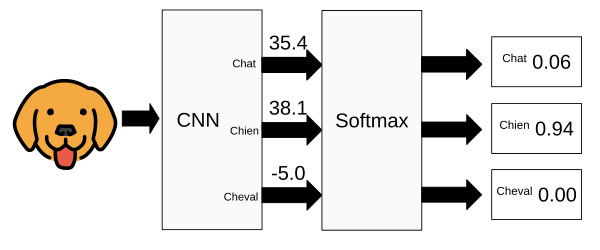
\includegraphics[width=0.55\textwidth]{./appunti_images/papers/fig_softmax.png}
\caption{Pipeline della Softmax: i logit grezzi (35.4, 38.1, -5.0) vengono trasformati in probabilità normalizzate (0.06, 0.94, 0.00). (Fonte: Wikimedia Commons)}
\label{fig:softmax_pipeline}
\end{figure}

\needspace{4\baselineskip}
\subsection{Esempio numerico}

\begin{notabox}[title={\textbf{Esempio: $\mathbf{z} = [2.0,\; 1.0,\; 0.1]$}}]
\textbf{Passo 1 -- calcolo degli esponenziali:}
\[
e^{2.0} \approx 7.389, \quad e^{1.0} \approx 2.718, \quad e^{0.1} \approx 1.105
\]

\textbf{Passo 2 -- somma totale:}
\[
S = 7.389 + 2.718 + 1.105 = 11.212
\]

\textbf{Passo 3 -- probabilità:}
\[
p_1 = \frac{7.389}{11.212} \approx 0.659, \quad
p_2 = \frac{2.718}{11.212} \approx 0.242, \quad
p_3 = \frac{1.105}{11.212} \approx 0.099
\]

Verifica: $0.659 + 0.242 + 0.099 = 1.000$ \checkmark

La classe 1 (con $z_1 = 2.0$ massimo) riceve la probabilità maggiore; l'ordine è preservato.
\end{notabox}

\needspace{4\baselineskip}
\subsection{Collegamento al Perceiver}

\begin{notabox}[title={\textbf{Softmax nel Perceiver}}]
La softmax compare in due punti del Perceiver IO:
\begin{enumerate}
  \item \textbf{Attention weights}: nella scaled dot-product attention, $\text{softmax}(\mathbf{Q}\mathbf{K}^\top/\sqrt{d_k})$ trasforma i punteggi di similarità in pesi di attenzione normalizzati.
  \item \textbf{Testa di classificazione}: l'ultimo strato del Perceiver per ImageNet applica una proiezione lineare $\mathbb{R}^D \to \mathbb{R}^{1000}$ seguita da softmax per ottenere la distribuzione sulle 1000 classi.
\end{enumerate}
\end{notabox}

% ---------------------------------------------------------------------------
\section{Fourier Features e Positional Encoding}
\label{app:fourier-theory}

I meccanismi di attenzione sono \textbf{invarianti per permutazione}: se si rimescolano gli elementi dell'input, l'output cambia solo nell'ordine ma non nel contenuto. Questo è un problema: il significato di un'immagine dipende dalla posizione spaziale dei pixel. La soluzione è iniettare esplicitamente l'informazione posizionale.

\needspace{4\baselineskip}
\subsection{Il problema: l'attenzione è cieca alla posizione}

Formalmente, per ogni permutazione $\sigma$ degli indici di input, la self-attention soddisfa:
\[
\text{Attention}(\mathbf{X}_{\sigma}) = \text{Attention}(\mathbf{X})_{\sigma}
\]
cioè l'output è la stessa permutazione dell'output originale. Il contenuto calcolato è identico. Senza positional encoding, ``il gatto mangia il topo'' e ``il topo mangia il gatto'' sarebbero rappresentati nello stesso modo.

\needspace{4\baselineskip}
\subsection{Tre approcci al positional encoding}

\begin{itemize}
  \item \textbf{Learned}: vettori di posizione appresi come parametri della rete (es.\ BERT). Flessibili ma non generalizzano a lunghezze non viste durante il training.
  \item \textbf{Sinusoidale (Vaswani et al., 2017)}: formula analitica con seni e coseni a frequenze diverse. Generalizza a sequenze arbitrariamente lunghe.
  \item \textbf{Fourier Features (Perceiver)}: generalizzazione multidimensionale del sinusoidale, applicabile a input arbitrari (immagini, audio, video) senza assumere struttura 1D.
\end{itemize}

\begin{figure}[htbp]
\centering
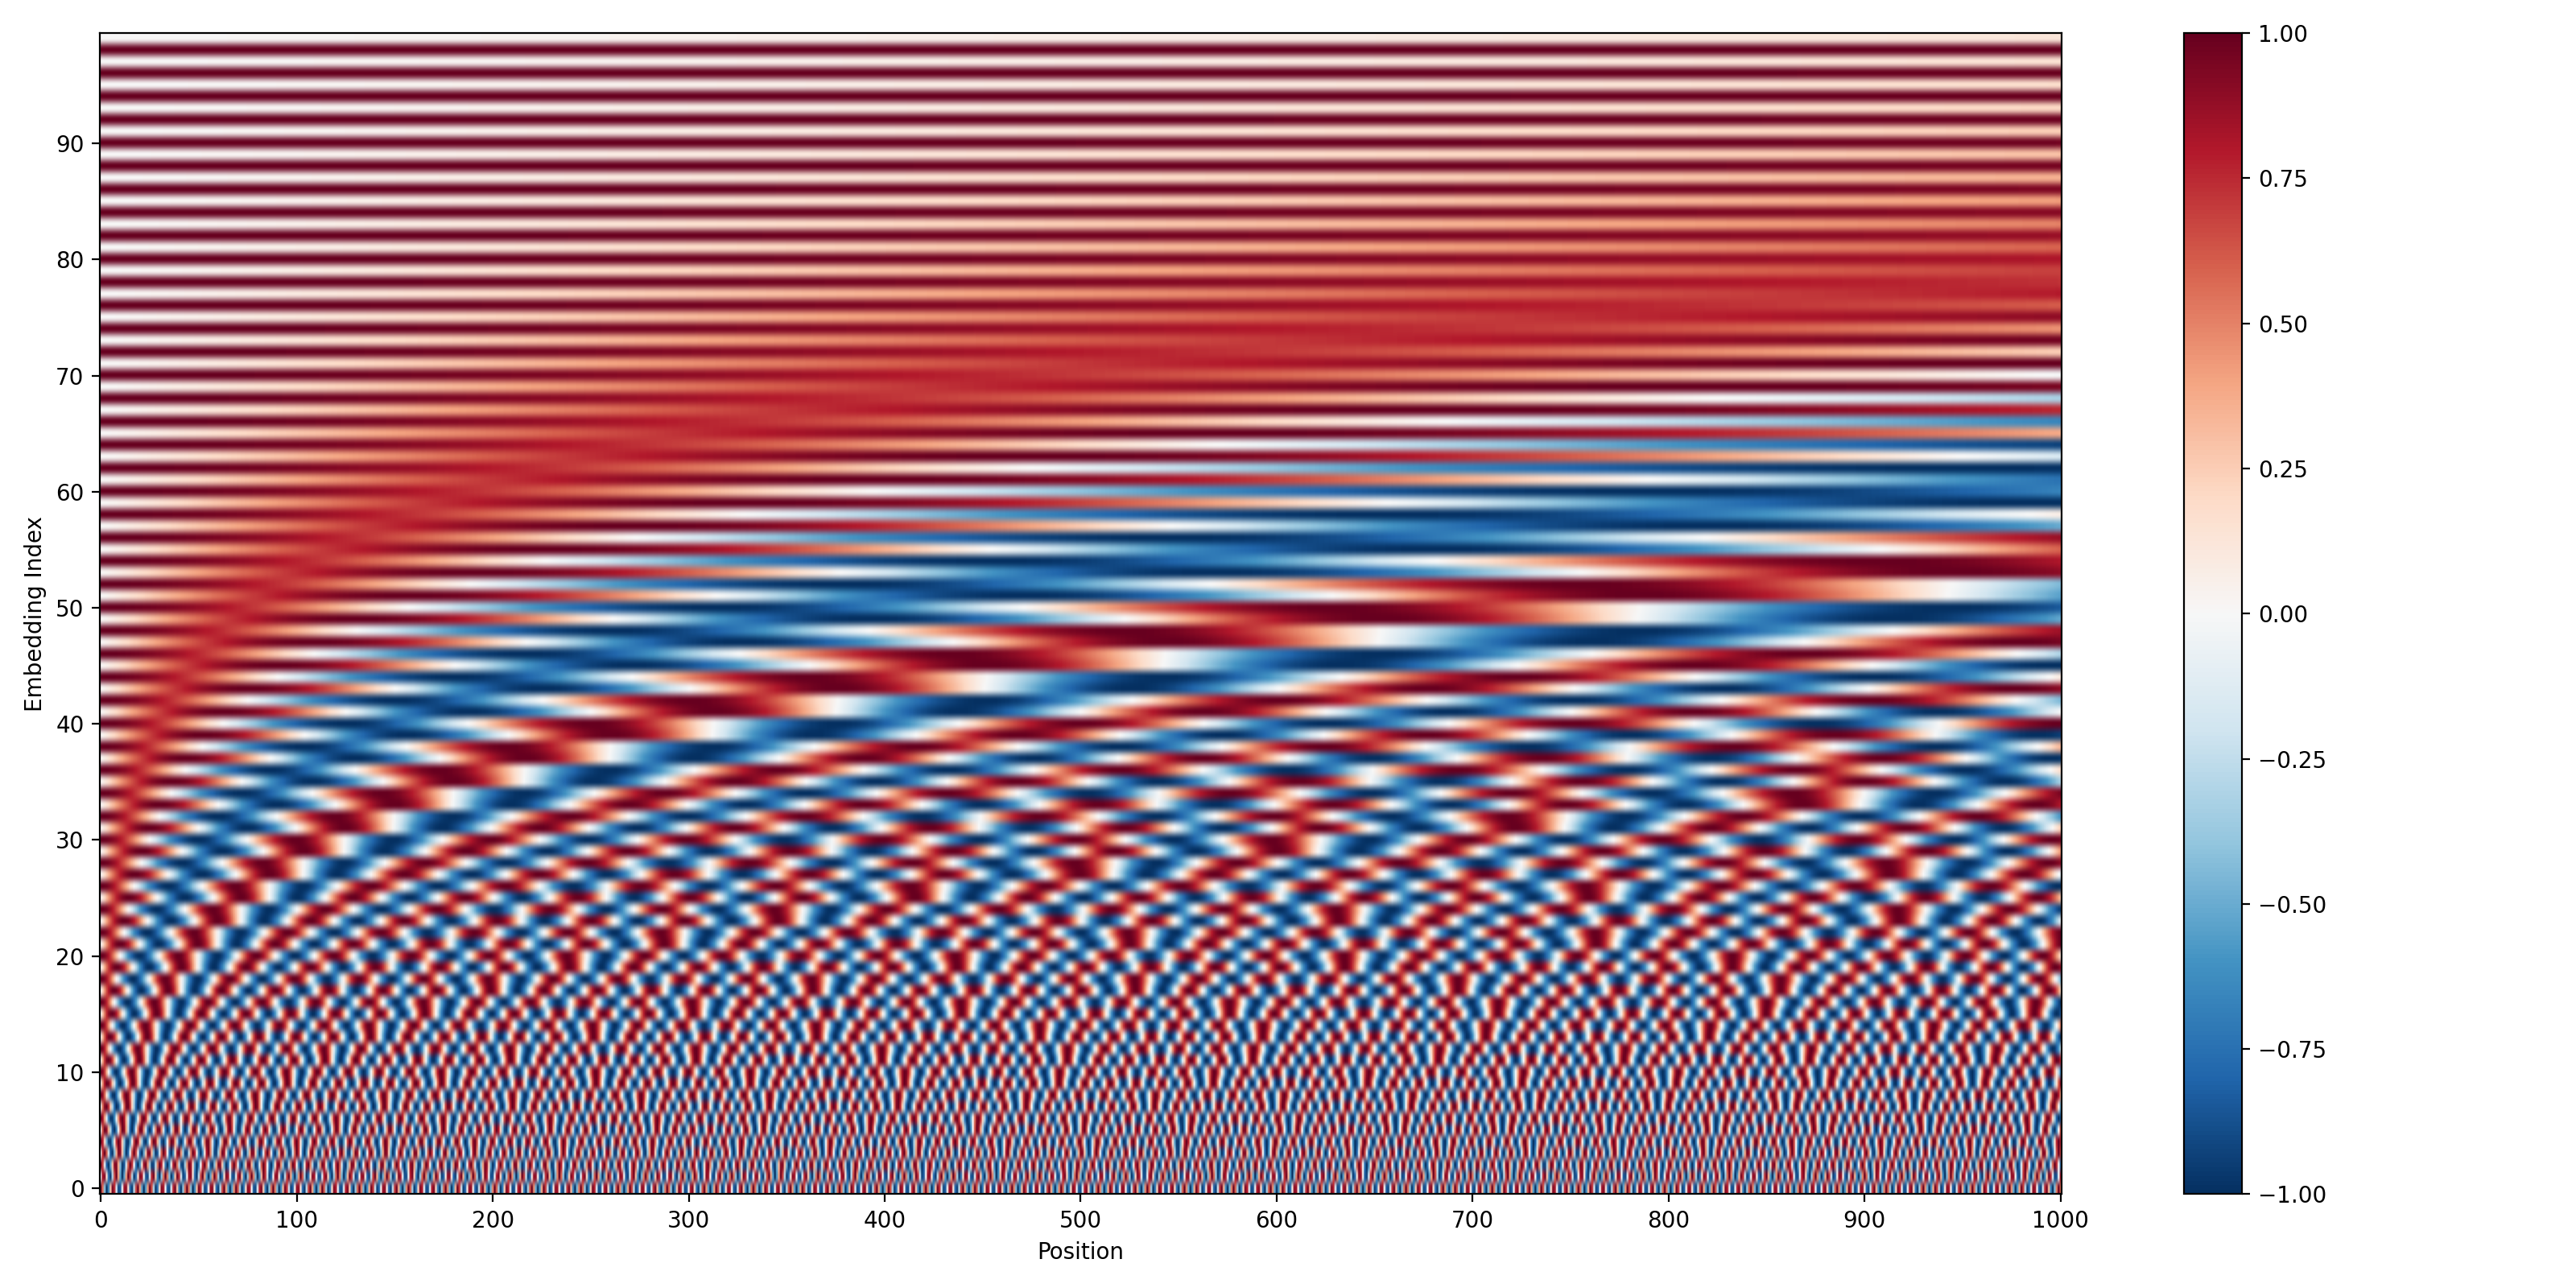
\includegraphics[width=0.65\textwidth]{./appunti_images/papers/fig_positional_encoding.png}
\caption{Heatmap del positional encoding sinusoidale: ogni riga è una posizione, ogni colonna una dimensione. Le basse dimensioni (in basso) oscillano rapidamente, le alte (in alto) lentamente. (Fonte: Wikimedia Commons)}
\label{fig:positional_encoding_heatmap}
\end{figure}

\needspace{4\baselineskip}
\subsection{Fourier Features nel Perceiver}

\begin{formulabox}[title={\textbf{Positional encoding con Fourier features (Perceiver)}}]
Per una coordinata normalizzata $x_d \in [-1, 1]$ lungo la dimensione $d$, con $K$ bande di frequenza:
\[
\text{PE}(x_d) = \bigl[\sin(f_1\,\pi\,x_d),\;\cos(f_1\,\pi\,x_d),\;\ldots,\;\sin(f_K\,\pi\,x_d),\;\cos(f_K\,\pi\,x_d),\;x_d\bigr]
\]
Le frequenze sono distribuite linearmente (o logaritmicamente): $f_k = 1, 2, \ldots, K$.\\
Il vettore finale si ottiene \textbf{concatenando} i contributi di tutte le dimensioni spaziali più i canali originali del segnale.
\end{formulabox}

\needspace{4\baselineskip}
\subsection{Perché frequenze multiple?}

Usare più frequenze crea una \textbf{rappresentazione multi-scala}:
\begin{itemize}
  \item \textbf{Frequenze basse} ($f_k$ piccolo): variano lentamente, codificano la posizione globale (dove mi trovo nell'immagine in senso ampio).
  \item \textbf{Frequenze alte} ($f_k$ grande): variano rapidamente, codificano la posizione locale (dettagli fini, distinguono pixel vicini).
\end{itemize}
L'insieme di tutte le frequenze garantisce che posizioni diverse producano rappresentazioni distinguibili.

\needspace{4\baselineskip}
\subsection{Perché concatenare la coordinata grezza $x_d$?}

I seni e coseni sono funzioni \textbf{periodiche}: $\sin(f_k\,\pi\,x_d) = \sin(f_k\,\pi\,(x_d + 2/f_k))$. Posizioni lontane potrebbero quindi avere encoding identici per alcune frequenze. Includere la coordinata grezza $x_d$ risolve questa ambiguità: due posizioni diverse hanno certamente encoding diversi grazie al contributo non-periodico.

\begin{notabox}[title={\textbf{Perceiver (concatenazione) vs Transformer (somma)}}]
\begin{itemize}
  \item \textbf{Transformer}: somma il positional encoding ai token: $\mathbf{x}_i' = \mathbf{x}_i + \text{PE}_i$. La posizione e il contenuto si \emph{mescolano} nelle stesse dimensioni.
  \item \textbf{Perceiver}: concatena il positional encoding: $\mathbf{x}_i' = [\mathbf{x}_i \;\|\; \text{PE}_i]$. Posizione e contenuto occupano dimensioni \emph{separate}; l'informazione originale è preservata intatta.
\end{itemize}
La concatenazione è più conservativa: il segnale originale non viene mai modificato, e la rete può scegliere autonomamente quanto peso dare alla posizione.
\end{notabox}

\needspace{4\baselineskip}
\subsection{Esempio numerico}

\begin{notabox}[title={\textbf{Esempio: $x = 0.3$, $K = 3$ bande, frequenze $f_1=1, f_2=2, f_3=4$}}]
\textbf{Calcolo delle componenti:}
\[
\sin(1 \cdot \pi \cdot 0.3) = \sin(0.942) \approx 0.809, \quad \cos(1 \cdot \pi \cdot 0.3) = \cos(0.942) \approx 0.588
\]
\[
\sin(2 \cdot \pi \cdot 0.3) = \sin(1.885) \approx 0.951, \quad \cos(2 \cdot \pi \cdot 0.3) = \cos(1.885) \approx -0.309
\]
\[
\sin(4 \cdot \pi \cdot 0.3) = \sin(3.770) \approx -0.588, \quad \cos(4 \cdot \pi \cdot 0.3) = \cos(3.770) \approx -0.809
\]

\textbf{Vettore finale:}
\[
\text{PE}(0.3) = [0.809,\;0.588,\;0.951,\;-0.309,\;-0.588,\;-0.809,\;0.3]
\]
7 componenti: $2K = 6$ sinusoidali + 1 coordinata grezza.
\end{notabox}

\needspace{4\baselineskip}
\subsection{Collegamento al Perceiver}

\begin{notabox}[title={\textbf{Fourier features nel Perceiver IO}}]
Le Fourier features permettono al Perceiver di essere \textbf{domain-agnostic}: la stessa architettura processa immagini, audio e video senza assumere nulla sulla struttura dell'input. Per un'immagine $224 \times 224$:
\begin{itemize}
  \item Ogni pixel ha coordinate normalizzate $(x, y) \in [-1,1]^2$.
  \item Con $K=64$ bande, il positional encoding ha $2 \times 2K = 256$ componenti sinusoidali + 2 coordinate grezze = 258 valori.
  \item Questi vengono concatenati ai canali RGB del pixel, ottenendo l'input finale al primo cross-attention.
\end{itemize}
Il framework teorico delle Fourier features come strumento di positional encoding per reti neurali su segnali continui è stato formalizzato da \textbf{Tancik et al.\ (2020)} in ``Fourier Features Let Networks Learn High Frequency Functions in Low Dimensional Domains'', dove si dimostra che mappare le coordinate di input a un embedding sinusoidale a banda larga migliora drasticamente la capacità delle MLP di rappresentare funzioni ad alta frequenza. Il Perceiver adotta questa idea estendendola a input multidimensionali arbitrari.
\end{notabox}

% ---------------------------------------------------------------------------
\section{Cross-Entropy Loss}
\label{app:cross-entropy}

La \textbf{cross-entropy loss} misura quanto la distribuzione di probabilità predetta dal modello differisce dalla distribuzione ``vera'' (tipicamente concentrata su una sola classe). È la funzione di loss standard per la classificazione.

\begin{formulabox}[title={\textbf{Cross-Entropy Loss}}]
Dato un vettore di probabilità predette $\mathbf{p} = (p_1, \ldots, p_K)$ e il vettore one-hot della classe vera $\mathbf{y} = (y_1, \ldots, y_K)$ (con $y_c = 1$ per la classe corretta $c$ e 0 altrove):
\[
\mathcal{L} = -\sum_{k=1}^{K} y_k \log(p_k) = -\log(p_c)
\]
Poiché $\mathbf{y}$ è one-hot, la somma collassa al solo termine della classe corretta.
\end{formulabox}

\needspace{4\baselineskip}
\subsection{Perché il logaritmo?}

\begin{itemize}
  \item Il logaritmo è \textbf{monotono crescente}: massimizzare $\log(p_c)$ equivale a massimizzare $p_c$.
  \item \textbf{Penalizzazione asimmetrica}: $-\log(0.01) \approx 4.6$ (predizione confident ma sbagliata), mentre $-\log(0.99) \approx 0.01$ (predizione quasi corretta). La perdita punisce fortemente le previsioni errate con alta confidenza.
  \item Emerge naturalmente dalla \textbf{stima di massima verosimiglianza}: minimizzare la cross-entropy equivale a massimizzare la log-likelihood del modello.
\end{itemize}

\begin{figure}[htbp]
\centering
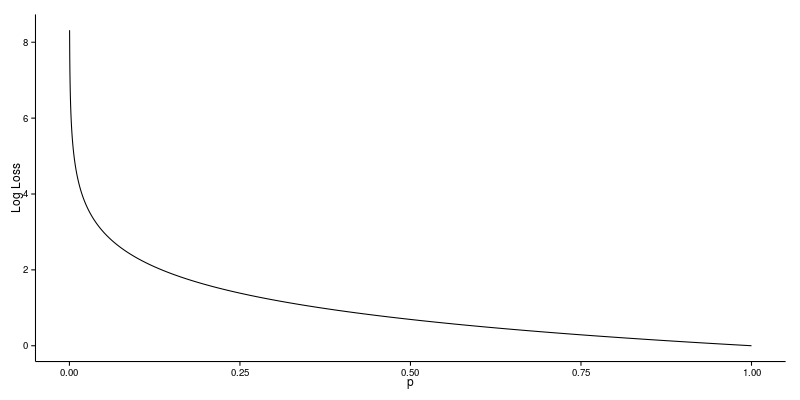
\includegraphics[width=0.50\textwidth]{./appunti_images/papers/fig_cross_entropy.png}
\caption{La funzione $-\log(p)$: quando la probabilità predetta $p$ è vicina a 1, la loss è quasi zero; quando $p \to 0$, la loss esplode verso $+\infty$. (Fonte: Wikimedia Commons)}
\label{fig:cross_entropy_curve}
\end{figure}

\needspace{4\baselineskip}
\subsection{Connessione con la softmax: gradiente pulito}

L'abbinamento softmax + cross-entropy produce un gradiente elegante. Se $\mathbf{z}$ è il logit pre-softmax e $c$ è la classe vera:

\begin{formulabox}[title={\textbf{Gradiente softmax + cross-entropy}}]
\[
\frac{\partial \mathcal{L}}{\partial z_k} = p_k - y_k
\]
Il gradiente rispetto al logit $z_k$ è semplicemente la \textbf{differenza tra probabilità predetta e target}. Non compaiono derivate di esponenziali o logaritmi: il calcolo si semplifica perfettamente.
\end{formulabox}

\begin{notabox}[title={\textbf{Intuizione del gradiente $p_k - y_k$}}]
Se il modello predice $p_c = 0.9$ per la classe corretta ($y_c = 1$), il gradiente è $0.9 - 1 = -0.1$: piccolo aggiustamento necessario. Se predice $p_c = 0.1$, il gradiente è $0.1 - 1 = -0.9$: grande aggiustamento necessario. Il segnale di apprendimento è proporzionale all'errore.
\end{notabox}

\needspace{4\baselineskip}
\subsection{Esempio numerico}

\begin{notabox}[title={\textbf{Esempio: classificazione a 3 classi, classe vera = 2}}]
\textbf{Probabilità predette:} $\mathbf{p} = [0.1,\; 0.7,\; 0.2]$

\textbf{Target one-hot:} $\mathbf{y} = [0,\; 1,\; 0]$ (classe 2, indice $k=2$)

\textbf{Calcolo della loss:}
\[
\mathcal{L} = -(0 \cdot \log 0.1 + 1 \cdot \log 0.7 + 0 \cdot \log 0.2) = -\log(0.7) \approx 0.357
\]

\textbf{Gradiente:} $\nabla_{\mathbf{z}} \mathcal{L} = [0.1 - 0,\; 0.7 - 1,\; 0.2 - 0] = [0.1,\; -0.3,\; 0.2]$

Il gradiente negativo sull'indice 2 ($-0.3$) indica che il modello deve aumentare il logit $z_2$: si sta imparando nella direzione corretta.
\end{notabox}

\needspace{4\baselineskip}
\subsection{Cross-entropy vs MSE per la classificazione}

\begin{notabox}[title={\textbf{Perché non usare l'MSE per la classificazione?}}]
L'MSE $\mathcal{L} = \frac{1}{K}\sum_k (p_k - y_k)^2$ può sembrare un'alternativa naturale, ma presenta due problemi:
\begin{enumerate}
  \item \textbf{Gradiente che svanisce con sigmoid/softmax}: quando $p_c \approx 0$ (predizione molto sbagliata), il gradiente dell'MSE diventa quasi zero (perché la derivata di sigmoid è piatta agli estremi). La cross-entropy non ha questo problema.
  \item \textbf{Trattamento simmetrico}: l'MSE penalizza allo stesso modo un errore su classe frequente e rara. La cross-entropy, tramite $-\log(p_c)$, cresce rapidamente quando $p_c \to 0$ indipendentemente dalla distribuzione delle altre classi.
\end{enumerate}
\end{notabox}

\needspace{4\baselineskip}
\subsection{Collegamento al Perceiver}

\begin{notabox}[title={\textbf{Cross-entropy nel Perceiver}}]
Il Perceiver IO per la classificazione su ImageNet usa la cross-entropy loss standard. Dopo il global average pooling sul latent array, una proiezione lineare produce 1000 logit, cui segue la softmax. La loss è $\mathcal{L} = -\log(p_c)$ dove $c$ è la classe ImageNet corretta. L'aggiornamento tramite backpropagation del gradiente $\mathbf{p} - \mathbf{y}$ si propaga attraverso tutti i 112 blocchi dell'architettura.
\end{notabox}

% ---------------------------------------------------------------------------
\section{Layer Normalization}
\label{app:layernorm}

La \textbf{Layer Normalization} (LN), introdotta da \textbf{Ba, Kiros \& Hinton (2016)} in ``Layer Normalization'' (arXiv:1607.06450), normalizza le attivazioni di ogni campione indipendentemente, riportando la media a 0 e la varianza a 1 lungo la dimensione delle feature. È il componente di stabilizzazione standard nei Transformer e nel Perceiver.

\begin{formulabox}[title={\textbf{Layer Normalization}}]
Dato il vettore di attivazioni $\mathbf{x} = (x_1, \ldots, x_D)$ per un singolo campione, con media $\mu$ e deviazione standard $\sigma$ calcolate sulle $D$ feature:
\[
\mu = \frac{1}{D}\sum_{j=1}^{D} x_j, \qquad
\sigma = \sqrt{\frac{1}{D}\sum_{j=1}^{D}(x_j - \mu)^2 + \varepsilon}
\]
\[
\text{LN}(\mathbf{x})_j = \gamma_j \cdot \frac{x_j - \mu}{\sigma} + \beta_j
\]
dove $\gamma_j$ e $\beta_j$ sono parametri \textbf{apprendibili} (scale e shift per feature), $\varepsilon \approx 10^{-5}$ evita la divisione per zero.
\end{formulabox}

\needspace{4\baselineskip}
\subsection{Layer Norm vs Batch Norm}

\begin{notabox}[title={\textbf{Differenza fondamentale tra LN e BatchNorm}}]
\begin{itemize}
  \item \textbf{Batch Normalization}: normalizza lungo la dimensione del \emph{batch}. Per ogni feature $j$, calcola $\mu_j$ e $\sigma_j$ su tutti i campioni del mini-batch. Dipende dalla dimensione del batch; instabile con batch piccoli.
  \item \textbf{Layer Normalization}: normalizza lungo la dimensione delle \emph{feature}. Per ogni campione, calcola $\mu$ e $\sigma$ su tutte le sue feature. Completamente indipendente dalla dimensione del batch.
\end{itemize}
La LN è quindi ideale per sequenze di lunghezza variabile e per situazioni in cui il batch è piccolo o la parallelizzazione cambia la struttura del batch.
\end{notabox}

\begin{figure}[htbp]
\centering
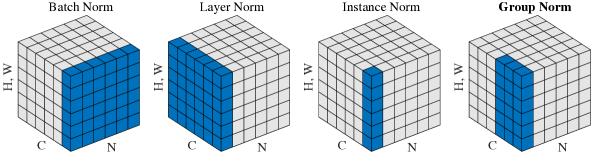
\includegraphics[width=0.80\textwidth]{./appunti_images/papers/fig_normalization_methods.png}
\caption{Confronto dei metodi di normalizzazione (da Wu \& He, 2018). I pixel blu indicano quali valori condividono le stesse statistiche ($\mu, \sigma$). BN normalizza lungo il batch ($N$); LN normalizza lungo le feature ($C, H, W$) per ogni singolo campione.}
\label{fig:normalization_methods}
\end{figure}

\needspace{4\baselineskip}
\subsection{Pattern pre-norm (usato nel Perceiver)}

Esistono due varianti di come integrare la LN in un blocco residuale:

\begin{formulabox}[title={\textbf{Pre-norm vs Post-norm}}]
\[
\text{Post-norm (Transformer originale):}\quad \mathbf{y} = \text{LN}\bigl(\mathbf{x} + f(\mathbf{x})\bigr)
\]
\[
\text{Pre-norm (GPT-2, Perceiver):}\quad \mathbf{y} = \mathbf{x} + f\bigl(\text{LN}(\mathbf{x})\bigr)
\]
\end{formulabox}

\begin{itemize}
  \item \textbf{Pre-norm}: la LN viene applicata \emph{prima} del sottoblocco. L'input residuale non normalizzato si somma direttamente all'output: il gradiente fluisce attraverso la skip connection senza essere modificato dalla LN. Più stabile per reti profonde.
  \item \textbf{Post-norm}: la LN viene applicata \emph{dopo} la somma residuale. Richiede warm-up più accurato del learning rate; può essere instabile nelle prime fasi del training.
\end{itemize}

\needspace{4\baselineskip}
\subsection{Parametri $\gamma$ e $\beta$}

Dopo la normalizzazione, i parametri appresi $\gamma$ (scale) e $\beta$ (shift) permettono alla rete di \textbf{annullare la normalizzazione} se necessario: se $\gamma_j = \sigma$ e $\beta_j = \mu$, la LN si riduce all'identità. In pratica, la rete impara il compromesso ottimale tra stabilità numerica e libertà espressiva.

\needspace{4\baselineskip}
\subsection{Esempio numerico}

\begin{notabox}[title={\textbf{Esempio: $\mathbf{x} = [1.0,\;2.0,\;3.0,\;4.0]$, $D=4$}}]
\textbf{Passo 1 -- media:}
\[
\mu = \frac{1.0 + 2.0 + 3.0 + 4.0}{4} = \frac{10.0}{4} = 2.5
\]

\textbf{Passo 2 -- varianza e deviazione standard} (con $\varepsilon = 0$ per semplicità):
\[
\sigma^2 = \frac{(1.0-2.5)^2 + (2.0-2.5)^2 + (3.0-2.5)^2 + (4.0-2.5)^2}{4}
= \frac{2.25 + 0.25 + 0.25 + 2.25}{4} = \frac{5.0}{4} = 1.25
\]
\[
\sigma = \sqrt{1.25} \approx 1.118
\]

\textbf{Passo 3 -- normalizzazione} (con $\gamma_j = 1$, $\beta_j = 0$):
\[
\hat{x}_1 = \frac{1.0 - 2.5}{1.118} \approx -1.342, \quad
\hat{x}_2 = \frac{2.0 - 2.5}{1.118} \approx -0.447
\]
\[
\hat{x}_3 = \frac{3.0 - 2.5}{1.118} \approx +0.447, \quad
\hat{x}_4 = \frac{4.0 - 2.5}{1.118} \approx +1.342
\]

\textbf{Risultato:} $\text{LN}(\mathbf{x}) \approx [-1.342,\;-0.447,\;+0.447,\;+1.342]$

Verifica: media $\approx 0$, varianza $\approx 1$ \checkmark
\end{notabox}

\needspace{4\baselineskip}
\subsection{Collegamento al Perceiver}

\begin{notabox}[title={\textbf{Layer Normalization nel Perceiver IO}}]
Il Perceiver usa il pattern \textbf{pre-norm} in ogni blocco. Con 8 cross-attention e 6 self-attention per layer, ciascuno con 2 sottoblocchi (attention + FFN), e 8 layer totali, si contano circa \textbf{112 operazioni di Layer Normalization}. Questo è il motivo per cui il training del Perceiver è stabile nonostante la profondità: ogni sottoblocco riceve input normalizzati, e il gradiente della loss può fluire attraverso le skip connections senza essere distorto.
\end{notabox}

% ---------------------------------------------------------------------------
\section{Funzioni di Attivazione}
\label{app:activations}

Le \textbf{funzioni di attivazione} introducono la non-linearità nelle reti neurali. Senza di esse, una composizione di trasformazioni lineari resterebbe lineare, e l'intera rete non potrebbe apprendere funzioni complesse. La scelta della funzione di attivazione influenza la velocità di convergenza, la stabilità del gradiente e le prestazioni finali.

\needspace{4\baselineskip}
\subsection{ReLU (Rectified Linear Unit)}

\begin{formulabox}[title={\textbf{ReLU}}]
\[
\text{ReLU}(x) = \max(0, x)
\]
Derivata: $\text{ReLU}'(x) = \begin{cases} 1 & x > 0 \\ 0 & x \leq 0 \end{cases}$
\end{formulabox}

\begin{itemize}
  \item \textbf{Vantaggi}: semplicissima da calcolare; non satura per $x > 0$; sparsità (molti neuroni a zero).
  \item \textbf{Problema ``dead neurons''}: se $x < 0$ per tutti i campioni del training, il gradiente è sempre 0 e il neurone smette di aggiornarsi permanentemente.
\end{itemize}

\begin{figure}[htbp]
\centering

\includegraphics[width=0.30\textwidth]{./appunti_images/papers/fig_relu.png}
\caption{Funzione ReLU: $\max(0, x)$. Lineare per $x > 0$, zero per $x \leq 0$.}
\end{figure}

\needspace{4\baselineskip}
\subsection{GELU (Gaussian Error Linear Unit)}

\begin{formulabox}[title={\textbf{GELU}}]
\[
\text{GELU}(x) = x \cdot \Phi(x)
\]
dove $\Phi(x) = \frac{1}{2}\!\left[1 + \text{erf}\!\left(\frac{x}{\sqrt{2}}\right)\right]$ è la CDF della distribuzione normale standard.

Approssimazione pratica:
\[
\text{GELU}(x) \approx 0.5\,x\,\bigl(1 + \tanh\!\bigl[\sqrt{2/\pi}\,(x + 0.044715\,x^3)\bigr]\bigr)
\]
\end{formulabox}

\begin{itemize}
  \item \textbf{Smooth}: a differenza di ReLU, GELU è differenziabile ovunque e non ha il punto angoloso in $x=0$.
  \item \textbf{Leggermente negativa per $x < 0$}: non è mai esattamente zero, i neuroni non muoiono completamente.
  \item \textbf{Usata in}: GPT-2, BERT, Perceiver IO e quasi tutti i Transformer moderni.
  \item \textbf{Riferimento}: proposta da \textbf{Hendrycks \& Gimpel (2016)} in ``Gaussian Error Linear Units (GELUs)''.
\end{itemize}

\begin{figure}[htbp]
\centering
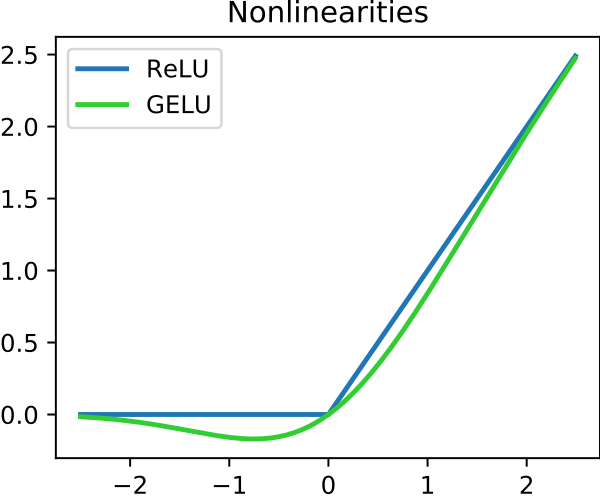
\includegraphics[width=0.40\textwidth]{./appunti_images/papers/fig_relu_gelu.png}
\caption{Confronto ReLU vs GELU. La ReLU (blu) ha un punto angoloso in $x=0$ e azzera bruscamente i valori negativi. La GELU (verde) è liscia, permette piccoli valori negativi e si avvicina all'identità per $x$ grandi. (Fonte: Wikimedia Commons)}
\label{fig:gelu_activations}
\end{figure}

\needspace{4\baselineskip}
\subsection{Sigmoid}

\begin{formulabox}[title={\textbf{Sigmoid}}]
\[
\sigma(x) = \frac{1}{1 + e^{-x}}, \qquad \sigma'(x) = \sigma(x)\,(1 - \sigma(x))
\]
\end{formulabox}

\begin{itemize}
  \item Output in $(0,1)$: interpretabile come probabilità.
  \item \textbf{Satura} per $|x|$ grandi: il gradiente $\sigma'(x) \to 0$, causando vanishing gradient.
  \item Usata nelle gate di LSTM e GRU (dove l'output in $[0,1]$ ha senso semantico come ``quanto aprire il gate'').
\end{itemize}

\begin{figure}[htbp]
\centering

\includegraphics[width=0.30\textwidth]{./appunti_images/papers/fig_sigmoid.png}
\caption{Funzione Sigmoid: output in $(0, 1)$, satura per $|x|$ grandi.}
\end{figure}

\needspace{4\baselineskip}
\subsection{Tanh}

\begin{formulabox}[title={\textbf{Tanh}}]
\[
\tanh(x) = \frac{e^x - e^{-x}}{e^x + e^{-x}}, \qquad \tanh'(x) = 1 - \tanh^2(x)
\]
\end{formulabox}

\begin{itemize}
  \item Output in $(-1, 1)$: centrato in zero, a differenza di sigmoid.
  \item Ancora soggetto a saturazione per $|x|$ grandi.
  \item Usata nelle celle di memoria LSTM e come attivazione nascosta nelle RNN classiche.
\end{itemize}

\begin{figure}[htbp]
\centering

\includegraphics[width=0.30\textwidth]{./appunti_images/papers/fig_tanh.png}
\caption{Funzione Tanh: output in $(-1, 1)$, centrata in zero, satura per $|x|$ grandi.}
\end{figure}

\needspace{4\baselineskip}
\subsection{Tabella comparativa}

{\def\LTcaptype{none}
\begin{longtable}{@{}
  >{\raggedright\arraybackslash}p{0.14\linewidth}
  >{\raggedright\arraybackslash}p{0.24\linewidth}
  >{\centering\arraybackslash}p{0.10\linewidth}
  >{\raggedright\arraybackslash}p{0.20\linewidth}
  >{\raggedright\arraybackslash}p{0.22\linewidth}@{}}
\toprule
\textbf{Funzione} & \textbf{Formula} & \textbf{Range} & \textbf{Derivata} & \textbf{Dove usata} \\
\midrule\endhead
\bottomrule\endlastfoot
ReLU & $\max(0,x)$ & $[0, +\infty)$ & 0 o 1 & CNN, MLP classici \\
GELU & $x\,\Phi(x)$ & $\approx(-0.17, +\infty)$ & smooth & GPT, BERT, Perceiver \\
Sigmoid & $1/(1+e^{-x})$ & $(0,1)$ & $\sigma(1-\sigma)$ & Gate LSTM/GRU, output binario \\
Tanh & $(e^x-e^{-x})/(e^x+e^{-x})$ & $(-1,1)$ & $1-\tanh^2$ & Celle LSTM, RNN classiche \\
\end{longtable}
}

\needspace{4\baselineskip}
\subsection{Perché GELU invece di ReLU nel Perceiver?}

\begin{notabox}[title={\textbf{GELU vs ReLU nelle architetture basate su attenzione}}]
\begin{enumerate}
  \item \textbf{Gradienti più fluidi}: GELU è smooth in $x=0$, favorendo ottimizzazione con Adam su reti molto profonde.
  \item \textbf{Nessun neurone morto}: la derivata di GELU non è mai esattamente zero, garantendo che tutti i neuroni ricevano segnale di aggiornamento.
  \item \textbf{Comportamento stocastico interpretabile}: $\text{GELU}(x) = x \cdot P(\text{mantieni il neurone})$, dove la probabilità segue una distribuzione gaussiana. Questo ha una connessione con il dropout stocastico.
  \item \textbf{Standard de facto}: BERT (Devlin, 2018) e GPT-2 (Radford, 2019) hanno dimostrato empiricamente che GELU supera ReLU nei Transformer; il Perceiver segue questa convenzione.
\end{enumerate}
\end{notabox}

\begin{notabox}[title={\textbf{Collegamento al Perceiver}}]
Il Perceiver IO usa GELU come attivazione nelle reti feed-forward (MLP) che seguono ogni blocco di attenzione. Ogni blocco MLP ha struttura: Linear $\to$ GELU $\to$ Linear, con espansione $4\times$ della dimensione nascosta (pattern standard dei Transformer).
\end{notabox}

% ---------------------------------------------------------------------------
\section{Residual Connections}
\label{app:residual}

Le \textbf{residual connections} (o skip connections) sono il meccanismo che permette di addestrare reti neurali molto profonde senza che i gradienti spariscano o le prestazioni degradino. Introdotte da He et al.\ con ResNet (2016, CVPR), sono ora un componente universale in ogni architettura profonda, incluso il Perceiver.

\needspace{4\baselineskip}
\subsection{Il problema: degradazione nelle reti profonde}

Aggiungere strati a una rete dovrebbe \emph{al massimo} mantenere le prestazioni (il nuovo strato può sempre imparare l'identità). In pratica, reti più profonde si comportavano peggio anche sul training set: la rete da 56 layer di VGG era più inaccurata di quella da 20 layer. Questo non è vanishing gradient (i pesi si aggiornano), ma \textbf{degradazione}: ottimizzare la funzione identità attraverso molti strati non lineari è sorprendentemente difficile.

\begin{formulabox}[title={\textbf{Residual Connection}}]
Invece di apprendere direttamente $H(\mathbf{x})$ (la trasformazione desiderata), la rete apprende il \textbf{residuo} $F(\mathbf{x}) = H(\mathbf{x}) - \mathbf{x}$:
\[
\mathbf{y} = F(\mathbf{x}) + \mathbf{x}
\]
Se il blocco non è utile, basta che $F(\mathbf{x}) \approx \mathbf{0}$ e la rete implementa l'identità.
\end{formulabox}

\begin{figure}[htbp]
\centering
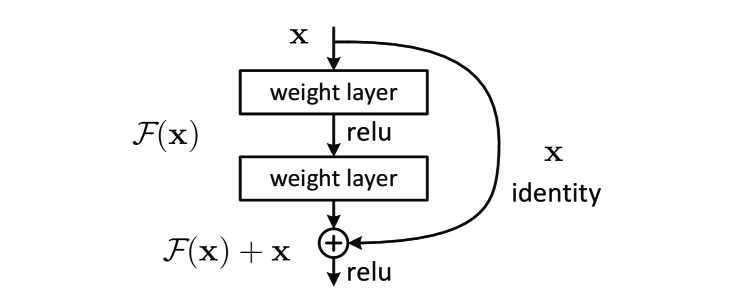
\includegraphics[width=0.30\textwidth]{./appunti_images/papers/fig_residual_block.png}
\caption{Il blocco residuale (da He et al., 2016): l'input $\mathbf{x}$ attraversa due weight layer per calcolare $F(\mathbf{x})$, poi viene sommato alla skip connection per ottenere $F(\mathbf{x}) + \mathbf{x}$.}
\label{fig:residual_block}
\end{figure}

\needspace{4\baselineskip}
\subsection{Perché funziona: flusso del gradiente}

\begin{notabox}[title={\textbf{Analisi del gradiente con e senza residual connection}}]
Considera un blocco con parametri $\theta$ e la loss $\mathcal{L}$:

\textbf{Senza residual:} $\mathbf{y} = F(\mathbf{x}; \theta)$
\[
\frac{\partial \mathcal{L}}{\partial \mathbf{x}} = \frac{\partial \mathcal{L}}{\partial \mathbf{y}} \cdot \frac{\partial F}{\partial \mathbf{x}}
\]
Il gradiente viene \emph{moltiplicato} per la Jacobiana di $F$. Con molti strati, se $\|\partial F / \partial \mathbf{x}\| < 1$, il prodotto si azzera (vanishing gradient).

\textbf{Con residual:} $\mathbf{y} = F(\mathbf{x}; \theta) + \mathbf{x}$
\[
\frac{\partial \mathcal{L}}{\partial \mathbf{x}} = \frac{\partial \mathcal{L}}{\partial \mathbf{y}} \cdot \left(\frac{\partial F}{\partial \mathbf{x}} + \mathbf{I}\right)
\]
Il termine $\mathbf{I}$ (matrice identità) garantisce che il gradiente non possa mai essere completamente zero: c'è sempre un percorso diretto attraverso la skip connection.
\end{notabox}

\needspace{4\baselineskip}
\subsection{Pattern pre-norm nel Perceiver}

Come discusso per la Layer Normalization (Appendice~\ref{app:layernorm}), il Perceiver combina residual connections e LN nel pattern \textbf{pre-norm}:

\begin{formulabox}[title={\textbf{Blocco residuale con pre-norm}}]
\[
\mathbf{y} = \mathbf{x} + f\!\bigl(\text{LN}(\mathbf{x})\bigr)
\]
\end{formulabox}

\begin{itemize}
  \item L'input $\mathbf{x}$ fluisce non modificato lungo la skip connection.
  \item Il sottoblocco $f$ riceve sempre input normalizzati: la LN stabilizza la scala delle attivazioni.
  \item Il gradiente di $\mathcal{L}$ rispetto a $\mathbf{x}$ ha sempre il termine additivo $+\mathbf{I}$: nessun vanishing gradient lungo la skip.
\end{itemize}

\needspace{4\baselineskip}
\subsection{Esempio numerico: confronto flusso del gradiente}

\begin{notabox}[title={\textbf{Esempio: 3 strati, gradiente senza e con residual}}]
Supponiamo 3 blocchi identici, ciascuno con Jacobiana $\partial F / \partial \mathbf{x} = 0.5\,\mathbf{I}$ (attenuazione del 50\% per strato).

\textbf{Senza residual:}
\[
\frac{\partial \mathcal{L}}{\partial \mathbf{x}_0} = (0.5)^3 \cdot \frac{\partial \mathcal{L}}{\partial \mathbf{y}_3} = 0.125 \cdot g
\]
Con 56 strati: $(0.5)^{56} \approx 1.4 \times 10^{-17}$ --- gradiente effettivamente zero.

\textbf{Con residual:}
\[
\frac{\partial \mathcal{L}}{\partial \mathbf{x}_0} \ni (0.5 + 1)^3 \cdot g = (1.5)^3 \cdot g = 3.375\,g
\]
Il gradiente non solo sopravvive: può anche \emph{crescere} lungo la skip. In pratica, i termini si bilanciano e il gradiente rimane in un range ragionevole anche per reti molto profonde.
\end{notabox}

\needspace{4\baselineskip}
\subsection{Collegamento al Perceiver}

\begin{notabox}[title={\textbf{Residual connections nel Perceiver IO}}]
Il Perceiver IO usa \textbf{112 residual connections} (stessa stima delle Layer Norm): una per ogni sottoblocco di attention e una per ogni FFN, in ogni layer. Senza di esse:
\begin{itemize}
  \item Il gradiente si azzerebbe prima di raggiungere i layer iniziali.
  \item La rete non potrebbe addestrare efficacemente il cross-attention iniziale (il punto critico dove le Fourier features dell'input incontrano il latent array).
  \item Il latent array non convergerebbe verso rappresentazioni stabili.
\end{itemize}
La stessa idea di ResNet --- il blocco deve imparare solo la \emph{correzione} rispetto all'input, non l'intera trasformazione --- si applica al contesto attention-based del Perceiver.
\end{notabox}

% ---------------------------------------------------------------------------
\section{Ottimizzatori}
\label{app:optimizers}

Gli \textbf{ottimizzatori} sono gli algoritmi che aggiornano i parametri di una rete neurale durante il training per minimizzare la funzione di perdita. La scelta dell'ottimizzatore ha un impatto enorme sulla velocità di convergenza, sulla stabilità e sulle prestazioni finali. Il Perceiver IO usa \textbf{LAMB}, una variante sofisticata di Adam progettata per il large batch training su TPU.

\needspace{4\baselineskip}
\subsection{SGD (Stochastic Gradient Descent)}

\begin{formulabox}[title={\textbf{SGD --- Aggiornamento dei pesi}}]
\[
W_{t+1} = W_t - \eta \nabla_W \mathcal{L}(W_t)
\]
dove $\eta$ è il \textbf{learning rate} (iperparametro fisso) e $\nabla_W \mathcal{L}$ è il gradiente della loss calcolato su un mini-batch.
\end{formulabox}

\begin{itemize}
  \item \textbf{Semplicità}: il meccanismo più elementare di ottimizzazione.
  \item \textbf{Problema: oscillazioni}. Nelle valli strette e allungate (tipiche della loss surface di reti profonde), il gradiente punta trasversalmente alla direzione di minimo, causando zig-zag lenti.
  \item \textbf{Problema: learning rate fisso per tutti i parametri}. Non tutti i parametri hanno la stessa sensibilità: pesi rari (es.\ embedding) ricevono aggiornamenti radi e ne trarrebbero vantaggio da step più grandi; pesi comuni ne trarrebbero vantaggio da step più piccoli.
  \item \textbf{Sensibilità all'iperparametro $\eta$}: troppo grande $\to$ divergenza; troppo piccolo $\to$ convergenza lentissima.
\end{itemize}

\begin{figure}[htbp]
\centering
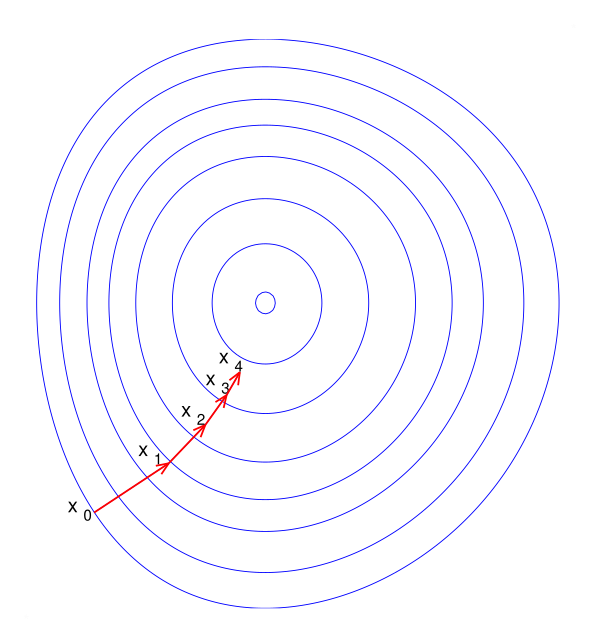
\includegraphics[width=0.35\textwidth]{./appunti_images/papers/fig_gradient_descent.png}
\caption{Discesa del gradiente: partendo da $x_0$, i pesi vengono aggiornati iterativamente seguendo la direzione opposta al gradiente fino a convergere verso il minimo. (Fonte: Wikimedia Commons)}
\label{fig:gradient_descent}
\end{figure}

\begin{notabox}[title={\textbf{Quando usare SGD?}}]
SGD (spesso con momentum e scheduling) rimane competitivo per le CNN su visione: ResNet e ViT spesso usano SGD+Momentum nella fase di fine-tuning su ImageNet. Nei Transformer e nelle reti di grandi dimensioni, Adam e le sue varianti sono quasi universalmente preferiti.
\end{notabox}

\needspace{4\baselineskip}
\subsection{SGD con Momentum}

Il \textbf{momentum} aggiunge un termine di inerzia all'aggiornamento, simulando una palla che rotola in discesa e accumula velocità nelle direzioni consistenti.

\begin{formulabox}[title={\textbf{SGD con Momentum}}]
\[
v_t = \beta\, v_{t-1} + \nabla_W \mathcal{L}(W_t)
\]
\[
W_{t+1} = W_t - \eta\, v_t
\]
dove $v_t$ è il \textbf{vettore di velocità} al passo $t$, $\beta \in [0,1)$ è il coefficiente di momentum (tipicamente $\beta = 0.9$) e $v_0 = \mathbf{0}$.
\end{formulabox}

\begin{notabox}[title={\textbf{Intuizione: la palla che rotola in discesa}}]
Immagina una palla che scende lungo un paesaggio collinare:
\begin{itemize}
  \item Senza momentum: ogni step è determinato solo dal pendio locale. La palla rimbalza su e giù nelle valli strette.
  \item Con momentum: la palla accumula velocità nelle direzioni in cui il gradiente è costantemente orientato (direzione del minimo) e si autocancella nelle direzioni oscillanti (pareti laterali della valle). Il risultato è una traiettoria più liscia e convergenza più rapida.
\end{itemize}
Il fattore $\beta = 0.9$ significa che la velocità precedente contribuisce al 90\% e il gradiente corrente al 10\% (scala): dopo $k$ passi, l'influenza del gradiente al passo $t-k$ è $\beta^k$. Con $\beta=0.9$ questa contribuzione dimezza ogni $\approx 7$ passi.
\end{notabox}

\needspace{4\baselineskip}
\subsection{Adam (Adaptive Moment Estimation)}

\textbf{Adam} (Kingma \& Ba, 2014) combina momentum (primo momento) e adattività per ogni parametro (secondo momento). È l'ottimizzatore più usato nel deep learning moderno.

\begin{formulabox}[title={\textbf{Adam --- Algoritmo completo}}]
\textbf{Inizializzazione:} $m_0 = 0$, $v_0 = 0$, $t = 0$.

Ad ogni passo $t$:

\textbf{1. Calcola il gradiente:}
\[
g_t = \nabla_W \mathcal{L}(W_t)
\]

\textbf{2. Aggiorna il primo momento (media dei gradienti):}
\[
m_t = \beta_1\, m_{t-1} + (1 - \beta_1)\, g_t
\]

\textbf{3. Aggiorna il secondo momento (varianza non centrata):}
\[
v_t = \beta_2\, v_{t-1} + (1 - \beta_2)\, g_t^2
\]

\textbf{4. Bias correction} (i momenti sono inizializzati a 0 e tendono a 0 all'inizio):
\[
\hat{m}_t = \frac{m_t}{1 - \beta_1^t}, \qquad \hat{v}_t = \frac{v_t}{1 - \beta_2^t}
\]

\textbf{5. Aggiornamento dei pesi:}
\[
W_{t+1} = W_t - \eta \cdot \frac{\hat{m}_t}{\sqrt{\hat{v}_t} + \epsilon}
\]

\textbf{Iperparametri tipici:} $\beta_1 = 0.9$, $\beta_2 = 0.999$, $\epsilon = 10^{-8}$, $\eta = 10^{-3}$ o $10^{-4}$.
\end{formulabox}

\begin{notabox}[title={\textbf{Perché Adam funziona bene?}}]
\begin{enumerate}
  \item \textbf{Learning rate adattivo per parametro}: $\hat{v}_t$ stima la varianza del gradiente. Parametri con gradienti grandi e frequenti ricevono step piccoli; parametri con gradienti piccoli e rari ricevono step grandi. Ideale per reti con embedding sparsi.
  \item \textbf{Momentum}: $\hat{m}_t$ è una media esponenzialmente pesata dei gradienti passati; riduce il rumore e accelera la convergenza nelle direzioni consistenti (come SGD+Momentum).
  \item \textbf{Bias correction}: nei primi passi, $m_t$ e $v_t$ sono vicini a zero (non sono ancora stati ``riscaldati''). Dividere per $(1-\beta^t)$ corregge questa inizializzazione a zero, evitando step troppo piccoli all'inizio.
  \item \textbf{Robustezza}: funziona bene con learning rate non troppo finemente accordati, a differenza di SGD.
\end{enumerate}
\end{notabox}

\needspace{4\baselineskip}
\subsubsection*{Esempio numerico: un passo di Adam}

\begin{notabox}[title={\textbf{Esempio: Adam al passo $t=1$ e $t=2$}}]
\textbf{Setup:} $W_0 = 0.5$, $\eta = 0.1$, $\beta_1 = 0.9$, $\beta_2 = 0.999$, $\epsilon = 10^{-8}$.

Supponi due gradienti consecutivi: $g_1 = 0.3$, $g_2 = -0.1$.

\medskip
\textbf{Passo $t=1$:}
\[
m_1 = 0.9 \cdot 0 + 0.1 \cdot 0.3 = 0.03
\]
\[
v_1 = 0.999 \cdot 0 + 0.001 \cdot (0.3)^2 = 0.001 \cdot 0.09 = 9 \times 10^{-5}
\]
\[
\hat{m}_1 = \frac{0.03}{1 - 0.9^1} = \frac{0.03}{0.1} = 0.3, \qquad
\hat{v}_1 = \frac{9 \times 10^{-5}}{1 - 0.999^1} = \frac{9 \times 10^{-5}}{0.001} = 0.09
\]
\[
W_1 = 0.5 - 0.1 \cdot \frac{0.3}{\sqrt{0.09} + 10^{-8}} = 0.5 - 0.1 \cdot \frac{0.3}{0.3} = 0.5 - 0.1 = \mathbf{0.4}
\]

\medskip
\textbf{Passo $t=2$:}
\[
m_2 = 0.9 \cdot 0.03 + 0.1 \cdot (-0.1) = 0.027 - 0.01 = 0.017
\]
\[
v_2 = 0.999 \cdot 9\times10^{-5} + 0.001 \cdot 0.01 \approx 8.991\times10^{-5} + 10^{-5} = 9.991\times10^{-5}
\]
\[
\hat{m}_2 = \frac{0.017}{1 - 0.81} = \frac{0.017}{0.19} \approx 0.0895, \qquad
\hat{v}_2 = \frac{9.991 \times 10^{-5}}{1 - 0.998001} \approx \frac{9.991\times10^{-5}}{0.001999} \approx 0.05
\]
\[
W_2 = 0.4 - 0.1 \cdot \frac{0.0895}{\sqrt{0.05}} = 0.4 - 0.1 \cdot \frac{0.0895}{0.2236} \approx 0.4 - 0.040 = \mathbf{0.360}
\]

\textbf{Osservazione:} al passo 2 il gradiente era negativo ($-0.1$) ma $\hat{m}_2 > 0$ perché il momento positivo del passo 1 domina ancora. Adam ``ricorda'' la direzione passata.
\end{notabox}

\begin{figure}[htbp]
\centering
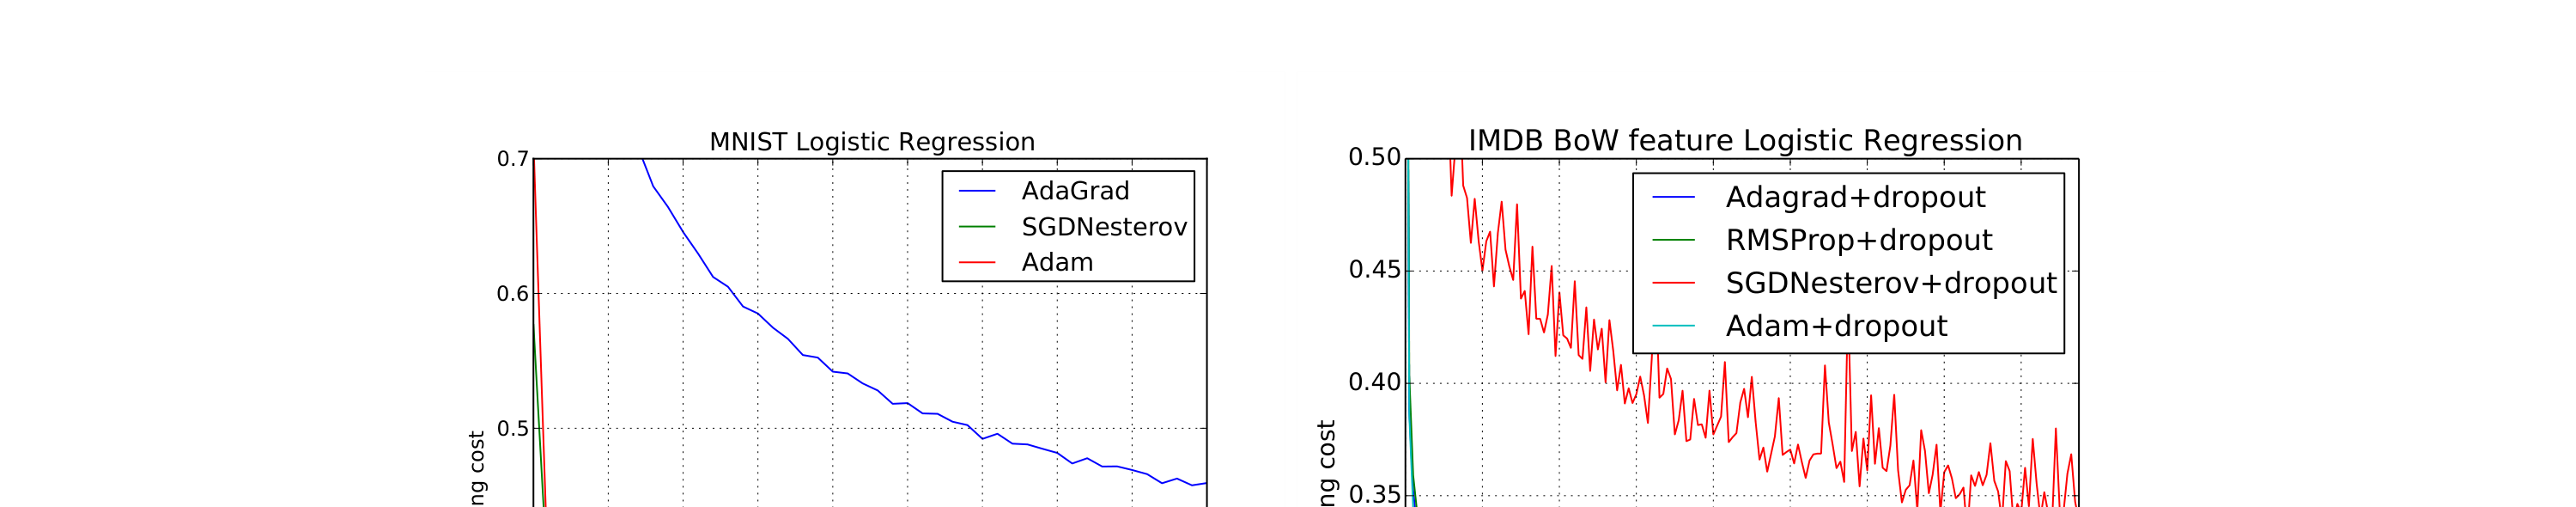
\includegraphics[width=0.85\textwidth]{./appunti_images/papers/fig_adam_convergence.png}
\caption{Convergenza degli ottimizzatori su regressione logistica (da Kingma \& Ba, 2014). Sinistra: MNIST. Destra: IMDB. Adam converge velocemente come SGD-Nesterov e molto meglio di Adagrad.}
\label{fig:adam_convergence}
\end{figure}

\begin{figure}[htbp]
\centering

\includegraphics[width=0.85\textwidth]{./appunti_images/papers/fig_adam_cnn.png}
\caption{Training cost su CNN (CIFAR-10) nei primi 3 epoch (sinistra) e su 45 epoch (destra). Adam e SGD convergono più velocemente di Adagrad sulle CNN (da Kingma \& Ba, 2014).}
\label{fig:adam_cnn}
\end{figure}

\needspace{4\baselineskip}
\subsection{AdamW (Adam con Weight Decay disaccoppiato)}

\textbf{AdamW} (Loshchilov \& Hutter, 2017) corregge un difetto di Adam: l'L2 regularization aggiunta al gradiente interagisce con l'adattività e non produce il vero weight decay.

\begin{formulabox}[title={\textbf{AdamW --- Differenza chiave da Adam}}]
\textbf{Adam con L2 reg.} aggiunge $\lambda W_t$ al gradiente \emph{prima} del calcolo dei momenti:
\[
g_t^{\text{reg}} = g_t + \lambda W_t \quad \to \quad \text{entra in } m_t \text{ e } v_t
\]

\textbf{AdamW} applica il weight decay \emph{dopo} l'aggiornamento adattivo, direttamente ai pesi:
\[
W_{t+1} = W_t - \eta \left(\frac{\hat{m}_t}{\sqrt{\hat{v}_t} + \epsilon} + \lambda\, W_t\right)
\]
Il termine $\lambda\, W_t$ scala uniformemente tutti i pesi verso zero, indipendentemente dalla storia dei gradienti.
\end{formulabox}

\begin{notabox}[title={\textbf{Perché il disaccoppiamento è importante?}}]
In Adam puro, $v_t$ accumula la magnitudine del gradiente $+ \lambda W_t$. I parametri con gradienti piccoli ma valori grandi ricevono un decay sproporzionatamente ridotto (il denominatore $\sqrt{\hat{v}_t}$ è piccolo, quindi l'adattività ``amplifica'' il decay). AdamW separa le due dinamiche: il decay è sempre $\lambda\, W_t$ indipendentemente dalla storia del gradiente. Il Perceiver usa weight decay $\lambda = 0.1$ con LAMB (che eredita questa correzione da AdamW).
\end{notabox}

\needspace{4\baselineskip}
\subsection{LAMB (Layer-wise Adaptive Moments for Batch training)}

\textbf{LAMB} (You et al., 2019) estende Adam con un \textbf{trust ratio per layer}, permettendo di usare batch size enormi (decine di migliaia di esempi su centinaia di acceleratori) senza instabilità. Il Perceiver IO usa LAMB con batch 1024 su 64 TPU per il training su ImageNet.

\begin{formulabox}[title={\textbf{LAMB --- Algoritmo}}]
\textbf{Step 1. Calcolo dell'update adattivo (come Adam):}
\[
\Delta W_t = \frac{\hat{m}_t}{\sqrt{\hat{v}_t} + \epsilon} + \lambda\, W_t
\]
(include weight decay disaccoppiato come AdamW)

\textbf{Step 2. Calcolo del trust ratio per layer $\ell$:}
\[
r_t^{(\ell)} = \frac{\|W_t^{(\ell)}\|}{\|\Delta W_t^{(\ell)}\|}
\]

\textbf{Step 3. Aggiornamento finale:}
\[
W_{t+1}^{(\ell)} = W_t^{(\ell)} - \eta \cdot r_t^{(\ell)} \cdot \Delta W_t^{(\ell)}
\]

Se $r_t^{(\ell)} = 1$, il comportamento è identico ad AdamW. Il trust ratio scala il learning rate effettivo di ogni layer in modo che lo step non superi la norma dei pesi correnti.
\end{formulabox}

\begin{notabox}[title={\textbf{Perché il trust ratio abilita il large batch training?}}]
Con batch size grande, il gradiente stimato è più accurato (meno rumore) ma i pesi di layer diversi hanno scale molto diverse:
\begin{itemize}
  \item I pesi del primo layer (processing dell'input grezzo) possono avere norme molto diverse dai pesi dell'ultimo layer (proiezione verso il numero di classi).
  \item Un learning rate globale che va bene per un layer è troppo grande o troppo piccolo per un altro.
\end{itemize}
Il trust ratio $r_t^{(\ell)} = \|W_t^{(\ell)}\| / \|\Delta W_t^{(\ell)}\|$ normalizza l'entità dello step rispetto alla scala dei pesi di ogni layer:
\begin{itemize}
  \item Se $\|\Delta W_t^{(\ell)}\| \ll \|W_t^{(\ell)}\|$: $r_t^{(\ell)} \gg 1$, lo step è amplificato (layer ``pigro'').
  \item Se $\|\Delta W_t^{(\ell)}\| \gg \|W_t^{(\ell)}\|$: $r_t^{(\ell)} \ll 1$, lo step è ridotto (protezione da esplosione).
\end{itemize}
Questo bilanciamento automatico per layer è ciò che consente la linearità nella relazione batch size $\leftrightarrow$ learning rate che LAMB sfrutta.
\end{notabox}

\begin{notabox}[title={\textbf{LAMB nel Perceiver IO}}]
Il paper del Perceiver (Jaegle et al., 2021) usa LAMB con le seguenti impostazioni per ImageNet:
\begin{itemize}
  \item Batch size: \textbf{1024} su \textbf{64 TPU} (batch per TPU: 16).
  \item Learning rate base: $2 \times 10^{-3}$.
  \item Weight decay: $\lambda = 0.1$.
  \item Schedule: LR piatto per 55 epoche, poi cosine decay per 55 epoche (110 totali).
  \item Gradient clipping: norma globale max 10 (prevenzione di esplosione del gradiente).
\end{itemize}
Perché non Adam? Con batch 1024 distribuito su molti dispositivi, Adam presenta instabilità al crescere del batch. LAMB garantisce stabilità mantenendo le stesse prestazioni finali.
\end{notabox}

\begin{figure}[htbp]
\centering

\includegraphics[width=0.50\textwidth]{./appunti_images/papers/fig_optimizer_saddle.png}
\caption{Confronto tra ottimizzatori su un punto di sella: SGD (in ciano) oscilla, mentre Momentum, NAG, Adagrad, Adadelta e RMSprop trovano percorsi più efficienti. (Fonte: Stanford CS231n)}
\label{fig:optimizer_saddle}
\end{figure}

\begin{figure}[htbp]
\centering
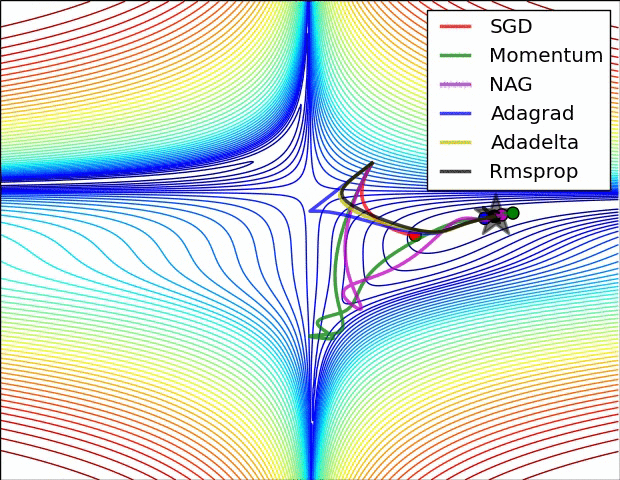
\includegraphics[width=0.50\textwidth]{./appunti_images/papers/fig_optimizer_contour.png}
\caption{Vista dall'alto delle traiettorie degli ottimizzatori sulle curve di livello della loss: SGD con Momentum converge rapidamente, mentre SGD puro oscilla. (Fonte: Stanford CS231n)}
\label{fig:optimizer_contour}
\end{figure}

\needspace{4\baselineskip}
\subsection{Learning Rate Scheduling}

Il learning rate non rimane costante durante il training: uno \textbf{schedule} lo varia per ottimizzare convergenza e prestazioni finali.

\begin{formulabox}[title={\textbf{Principali strategie di scheduling}}]
\textbf{Warmup lineare} (da 0 a $\eta_{\max}$ in $T_w$ passi):
\[
\eta_t = \eta_{\max} \cdot \frac{t}{T_w}, \quad t \leq T_w
\]

\textbf{Step decay} (riduzione di un fattore $\gamma$ ogni $T_s$ epoche):
\[
\eta_t = \eta_0 \cdot \gamma^{\lfloor t / T_s \rfloor}
\]

\textbf{Cosine decay} (da $\eta_{\max}$ a $\eta_{\min}$ in $T_c$ passi):
\[
\eta_t = \eta_{\min} + \frac{1}{2}(\eta_{\max} - \eta_{\min})\left(1 + \cos\!\left(\frac{\pi\, t}{T_c}\right)\right)
\]
\end{formulabox}

\begin{notabox}[title={\textbf{Warmup: perché partire da un LR basso?}}]
All'inizio del training, i momenti $m_t$ e $v_t$ di Adam/LAMB sono inizializzati a zero e non riflettono ancora la curvatura reale della loss. Un learning rate alto in questa fase può causare aggiornamenti instabili che danneggiano l'inizializzazione dei pesi. Il warmup permette ai momenti di ``scaldarsi'' prima che l'ottimizzatore inizi a fare passi ampi.

Il Perceiver usa un flat LR di $2\times10^{-3}$ per 55 epoche (fase di esplorazione) seguito da cosine decay per 55 epoche (fase di raffinamento verso il minimo).
\end{notabox}

\begin{figure}[htbp]
\centering
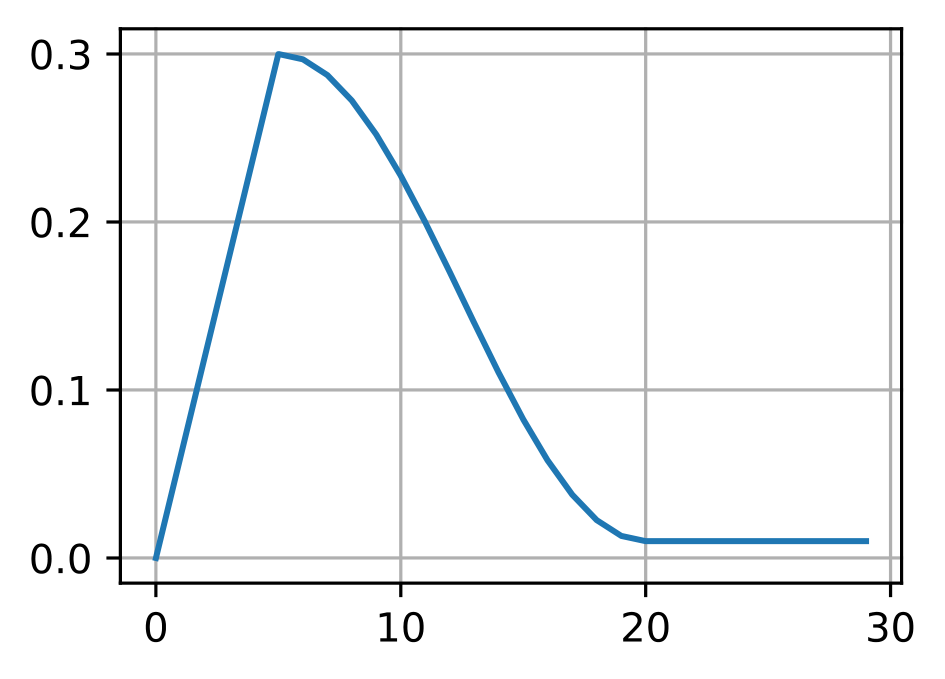
\includegraphics[width=0.50\textwidth]{./appunti_images/papers/fig_lr_cosine_warmup.png}
\caption{Schedule di learning rate con warmup lineare + cosine decay (da d2l.ai, Apache 2.0). Il learning rate cresce linearmente durante il warmup, poi decresce con un profilo cosinusoidale.}
\label{fig:lr_cosine_warmup}
\end{figure}

\needspace{4\baselineskip}
\subsection{Tabella comparativa degli ottimizzatori}

{\def\LTcaptype{none}
\begin{longtable}{@{}
  >{\raggedright\arraybackslash}p{0.14\linewidth}
  >{\raggedright\arraybackslash}p{0.22\linewidth}
  >{\raggedright\arraybackslash}p{0.18\linewidth}
  >{\raggedright\arraybackslash}p{0.16\linewidth}
  >{\raggedright\arraybackslash}p{0.20\linewidth}@{}}
\toprule
\textbf{Ottimizzatore} & \textbf{Idea chiave} & \textbf{LR adattivo} & \textbf{Momentum} & \textbf{Caso d'uso tipico} \\
\midrule\endhead
\bottomrule\endlastfoot
SGD & Gradiente scalato da $\eta$ & No (globale) & No & CNN classiche \\
SGD+Momentum & Inerzia accumulate & No (globale) & Sì & ResNet su ImageNet \\
Adam & Momento + varianza & Sì (per param) & Sì & Transformer, NLP \\
AdamW & Adam + decoupled decay & Sì (per param) & Sì & BERT, GPT, ViT \\
LAMB & AdamW + trust ratio & Sì (per param) & Sì & Large batch, TPU (Perceiver) \\
\end{longtable}
}

% ---------------------------------------------------------------------------
\section{Perceptrone}
\label{app:perceptrone}

Il \textbf{perceptrone} è il mattone fondamentale di ogni rete neurale: un classificatore lineare binario.
Capire il perceptrone è essenziale perché ogni neurone nelle architetture successive --- fino al Perceiver --- ne ricalca la struttura base (somma ponderata + attivazione).

\needspace{4\baselineskip}
\subsection{Struttura}

\begin{figure}[htbp]
\centering

\includegraphics[width=0.55\textwidth]{./appunti_images/media/image1.png}
\caption{Schema di un perceptrone: input, pesi, somma ponderata e funzione di attivazione.}
\end{figure}

Un perceptrone riceve $n$ input $x_1, \ldots, x_n$, ciascuno moltiplicato per un peso $w_i$, somma il tutto con un bias $b$ e applica una funzione di attivazione a gradino.

\begin{formulabox}[title={\textbf{Output del Perceptrone}}]
\[
y = f\!\left(\sum_{i=1}^{n} w_{i}\, x_{i} + b\right)
\qquad\text{con }
f(z) = \begin{cases} 1 & z \ge 0 \\ 0 & z < 0 \end{cases}
\]
\end{formulabox}

\begin{figure}[htbp]
\centering
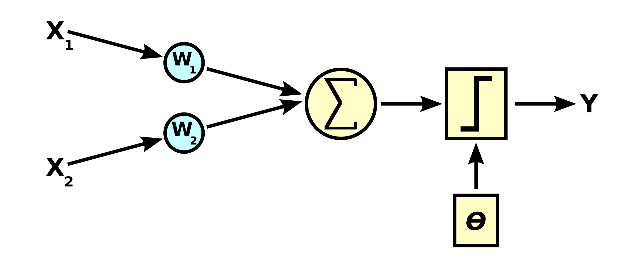
\includegraphics[width=0.55\textwidth]{./appunti_images/media/image2.png}
\caption{Struttura di un neurone artificiale: input $x_i$, pesi $w_i$, somma ponderata e funzione di attivazione.}
\end{figure}

\needspace{4\baselineskip}
\subsection{Esempio pratico}

\begin{notabox}[title={\textbf{Esempio: indossare la giacca?}}]
\textbf{Input:} Temperatura $x_1 = 0.5$ (18\textdegree C normalizzato), Pioggia $x_2 = 0$.\\
\textbf{Pesi:} $w_1 = -0.7$, $w_2 = 1.0$, $b = 0.1$.

\[
z = (-0.7)(0.5) + (1.0)(0) + 0.1 = -0.25
\]

Poiché $z < 0$, la funzione a gradino restituisce $y = 0$ $\rightarrow$ ``Non indossare la giacca''.

\medskip
\textbf{Contro-esempio:} se invece piovesse ($P = 1$): $z = -0.35 + 1.0 + 0.1 = 0.75 > 0 \;\Rightarrow\; y = 1$: \textbf{indossa la giacca}.
\end{notabox}

\needspace{4\baselineskip}
\subsection{Training}

Addestrare il perceptrone significa aggiustare i pesi per ridurre l'errore di classificazione.

\begin{formulabox}[title={\textbf{Regola di aggiornamento dei pesi e del bias}}]
\[
w_j^{(k+1)} = w_j^{(k)} + \lambda \bigl(y_i - \hat{y}_i^{(k)}\bigr)\, x_{ij}
\qquad\qquad
b^{(k+1)} = b^{(k)} + \lambda \bigl(y_i - \hat{y}_i^{(k)}\bigr)
\]
\end{formulabox}

Il \textbf{learning rate} $\lambda \in (0,1]$ controlla l'ampiezza degli aggiustamenti: un $\lambda$ alto permette modifiche ampie, un $\lambda$ basso modifiche fini. Spesso si usa un $\lambda$ decrescente durante il training.

\begin{notabox}[title={\textbf{Teorema di convergenza del perceptrone}}]
Se i dati sono \textbf{linearmente separabili}, la regola di aggiornamento del perceptrone converge in un numero finito di passi, indipendentemente dall'inizializzazione dei pesi. Questo risultato, dimostrato da Rosenblatt (1962), garantisce che l'algoritmo troverà sempre una soluzione --- ma \emph{solo} quando tale soluzione esiste.
\end{notabox}

\begin{notabox}[title={\textbf{Esempio numerico: un passo di training}}]
Supponiamo $x_1 = 1$, $x_2 = 0$, target $= 1$, output $= 0$, $\lambda = 0.1$:

\[
\text{errore} = \text{target} - \text{output} = 1 - 0 = 1
\]
\[
w_1^{\text{new}} = w_1^{\text{old}} + 0.1 \cdot 1 \cdot 1 = w_1^{\text{old}} + 0.1
\qquad
w_2^{\text{new}} = w_2^{\text{old}} + 0.1 \cdot 1 \cdot 0 = w_2^{\text{old}} \quad\text{(invariato, perché } x_2 = 0\text{)}
\]
Il peso $w_1$ aumenta perché l'input $x_1$ avrebbe dovuto contribuire all'attivazione ma non lo ha fatto sufficientemente. Il peso $w_2$ resta invariato perché il corrispondente input era nullo: non ha responsabilità nell'errore.
\end{notabox}

\begin{figure}[htbp]
\centering

\includegraphics[width=0.55\textwidth]{./appunti_images/media/image4.png}
\caption{Rappresentazione geometrica del confine di decisione del perceptrone.}
\end{figure}

\needspace{4\baselineskip}
\subsection{Limiti: il problema XOR}

Il perceptrone converge solo su problemi \textbf{linearmente separabili}. La funzione XOR non lo è: nessuna retta nel piano separa le classi.

\begin{notabox}[title={\textbf{Tavola di verità dello XOR}}]
\begin{center}
\begin{tabular}{cc|c}
$x_1$ & $x_2$ & XOR \\
\hline
0 & 0 & 0 \\
0 & 1 & 1 \\
1 & 0 & 1 \\
1 & 1 & 0 \\
\end{tabular}
\end{center}
Non esiste nessuna retta nel piano $(x_1, x_2)$ che separi i punti con output 0 da quelli con output 1. Questo limite, evidenziato da Minsky e Papert (1969), fu superato solo con l'introduzione dei \textbf{perceptroni multi-strato} (reti feedforward).
\end{notabox}

\begin{figure}[htbp]
\centering
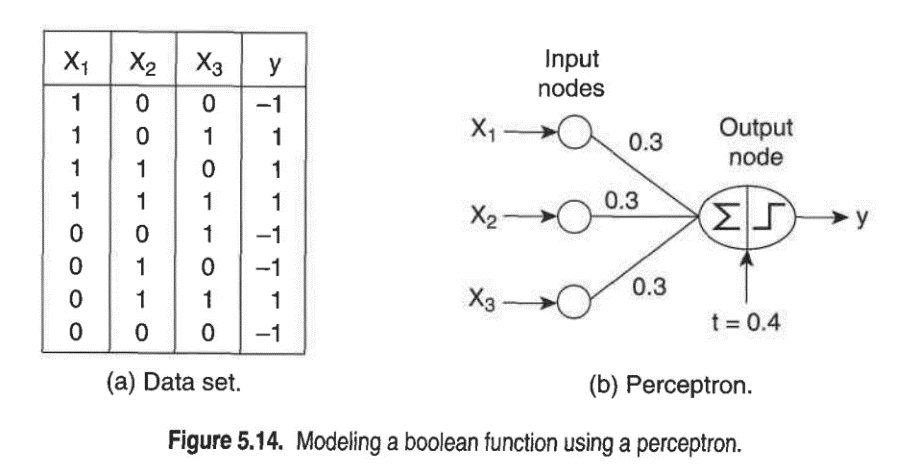
\includegraphics[width=0.45\textwidth]{./appunti_images/media/image5.png}
\hfill

\includegraphics[width=0.45\textwidth]{./appunti_images/media/image6.png}
\caption{Sinistra: distribuzione dei punti XOR nel piano (non linearmente separabili). Destra: soluzione tramite rete multi-strato.}
\end{figure}

Per superare questo limite è necessario introdurre \textbf{hidden layer} aggiuntivi, ottenendo le reti neurali multi-strato.

% ---------------------------------------------------------------------------

\section{Reti Neurali Feed-Forward}
\label{app:feedforward}

Le \textbf{reti feed-forward} (multi-layer perceptron, MLP) estendono il perceptrone aggiungendo strati nascosti tra input e output. L'informazione fluisce in una sola direzione, senza cicli. Il meccanismo di training qui descritto --- forward propagation, loss, backpropagation --- è lo stesso usato in CNN, Transformer e Perceiver.

\begin{notabox}[title={\textbf{Teorema dell'approssimatore universale (Cybenko, 1989)}}]
Una rete feedforward con \emph{un solo hidden layer} e un numero sufficiente di neuroni con funzione di attivazione non lineare può approssimare qualsiasi funzione continua su un compatto con precisione arbitraria. Questo giustifica teoricamente l'uso degli MLP --- ma non dice \emph{quanti} neuroni servano: in pratica, reti \textbf{profonde} (più layer) sono molto più efficienti di reti larghe (un solo layer enorme).
\end{notabox}

\needspace{4\baselineskip}
\subsection{Architettura}

\begin{figure}[htbp]
\centering
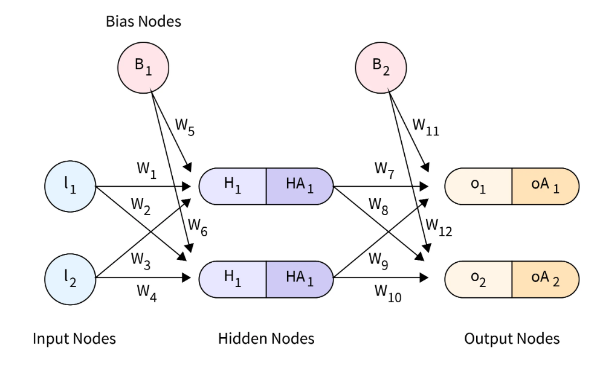
\includegraphics[width=0.55\textwidth]{./appunti_images/media/image7.png}
\caption{Architettura di una rete neurale feed-forward con input layer, hidden layer e output layer.}
\end{figure}

\begin{itemize}
\item \textbf{Input Layer:} accetta i dati e li trasmette. Nessun parametro apprendibile.
\item \textbf{Hidden Layer:} eseguono trasformazioni non lineari (ReLU, sigmoid, ecc.) e apprendono rappresentazioni intermedie.
\item \textbf{Output Layer:} produce la previsione finale (softmax per classificazione, lineare per regressione).
\end{itemize}

\needspace{4\baselineskip}
\subsection{Forward Propagation}

Per ogni neurone, si calcola l'input netto $z$ e poi l'output tramite la funzione di attivazione $f$:

\begin{formulabox}[title={\textbf{Forward pass di un neurone}}]
\[
z = \sum_{i} w_i \, x_i + b \qquad\qquad \hat{y} = f(z)
\]
\end{formulabox}

\needspace{4\baselineskip}
\subsection{Loss Function: MSE}
\label{app:loss}

Per misurare l'errore tra previsione e target si usa una loss function. Per problemi di regressione, la Mean Squared Error:

\begin{formulabox}[title={\textbf{Mean Squared Error}}]
\[
E = \frac{1}{2}\sum_{i}\bigl(y_i - \hat{y}_i\bigr)^{2}
\]
\end{formulabox}

Per problemi di \textbf{classificazione multi-classe} si usa la \textbf{Cross-Entropy Loss}:

\[
\mathcal{L}_{\text{CE}} = -\sum_{k=1}^{K} y_k \log \hat{y}_k
\]
dove $K$ è il numero di classi. La cross-entropy è la loss standard usata nei Transformer, nel ViT e nel Perceiver.

\needspace{4\baselineskip}
\subsection{Backpropagation}
\label{app:backprop}

La backpropagation calcola i gradienti della loss rispetto a ogni peso, propagando l'errore dall'output verso l'input tramite la \textbf{regola della catena}.

\begin{formulabox}[title={\textbf{I 6 passi della Backpropagation}}]
\begin{enumerate}
\item \textbf{Gradiente rispetto all'output:} $\;\dfrac{\partial E}{\partial \hat{y}} = \hat{y} - y$
\item \textbf{Gradiente rispetto all'input netto:} $\;\dfrac{\partial E}{\partial z} = \dfrac{\partial E}{\partial \hat{y}} \cdot f'(z)$
\item \textbf{Gradiente rispetto ai pesi:} $\;\dfrac{\partial E}{\partial w} = \dfrac{\partial E}{\partial z} \cdot x$
\item \textbf{Gradiente rispetto al bias:} $\;\dfrac{\partial E}{\partial b} = \dfrac{\partial E}{\partial z}$
\item \textbf{Propagazione all'indietro:} ripetere i passi 1--4 per ogni layer, dal fondo verso l'input
\item \textbf{Aggiornamento dei pesi:} $\;w_{\text{new}} = w_{\text{old}} - \eta \,\dfrac{\partial E}{\partial w}$, $\;\;b_{\text{new}} = b_{\text{old}} - \eta \,\dfrac{\partial E}{\partial b}$
\end{enumerate}
\end{formulabox}

\begin{notabox}[title={\textbf{In parole semplici: la backpropagation come catena di montaggio}}]
Immagina una \textbf{catena di montaggio} dove ogni operaio (neurone) modifica il pezzo. Se il prodotto finale è difettoso (loss alta), il controllo qualità (backpropagation) risale la catena chiedendo a ogni operaio: \emph{``Quanto sei responsabile di questo difetto?''}. L'operaio che ha contribuito di più riceve la correzione più grande (gradiente più grande). La \textbf{chain rule} è il meccanismo che permette di ``scomporre'' la responsabilità strato per strato.
\end{notabox}

\begin{notabox}[title={\textbf{Esempio numerico: backpropagation su rete semplice}}]
Rete con 1 input $x = 2$, 1 hidden neuron con ReLU, 1 output con identità. Pesi: $w_1 = 0.5$, $w_2 = -0.3$, bias $= 0$. Target: $y_{\text{true}} = 1$.

\textbf{Forward:} $z_1 = 0.5 \times 2 = 1.0$, $a_1 = \text{ReLU}(1.0) = 1.0$, $\hat{y} = -0.3 \times 1.0 = -0.3$.
\textbf{Loss MSE:} $\mathcal{L} = (-0.3 - 1)^2 = 1.69$.

\textbf{Backward:}
\begin{itemize}
\item $\frac{\partial \mathcal{L}}{\partial \hat{y}} = 2(-0.3 - 1) = -2.6$
\item $\frac{\partial \mathcal{L}}{\partial w_2} = -2.6 \times a_1 = -2.6$
\item $\frac{\partial \mathcal{L}}{\partial a_1} = -2.6 \times w_2 = -2.6 \times (-0.3) = 0.78$
\item $\frac{\partial \mathcal{L}}{\partial z_1} = 0.78 \times \text{ReLU}'(1.0) = 0.78$
\item $\frac{\partial \mathcal{L}}{\partial w_1} = 0.78 \times x = 0.78 \times 2 = 1.56$
\end{itemize}
\textbf{Aggiornamento} ($\eta = 0.01$): $w_2 \leftarrow -0.3 - 0.01 \times (-2.6) = -0.274$, $w_1 \leftarrow 0.5 - 0.01 \times 1.56 = 0.4844$.
\end{notabox}

\begin{figure}[htbp]
\centering

\includegraphics[width=0.60\textwidth]{./appunti_images/media/image8.png}
\caption{Schema della backpropagation in una rete feed-forward: l'errore viene propagato dall'output verso l'input attraverso gli hidden layer.}
\end{figure}

Le reti feed-forward trattano ogni input in modo indipendente, senza nozione di ordine o tempo. Per dati \textbf{sequenziali} (testo, audio, serie temporali) servono architetture con memoria: le reti neurali ricorrenti.

% ---------------------------------------------------------------------------

\section{Reti Neurali Ricorrenti (RNN)}
\label{app:rnn}

Le \textbf{RNN} estendono le reti feed-forward aggiungendo un \textbf{loop nello stato nascosto}: l'output di $h_{t-1}$ viene reinserito come input al passo successivo, creando una forma di \textbf{memoria}. Questo le rende adatte a dati sequenziali.

\needspace{4\baselineskip}
\subsection{Il loop nello stato nascosto}

\begin{figure}[htbp]
\centering
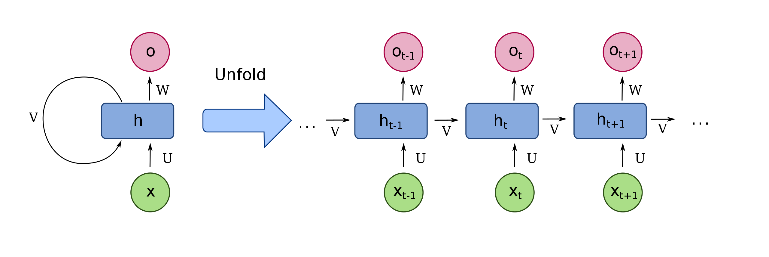
\includegraphics[width=0.55\textwidth]{./appunti_images/media/image9.png}
\caption{Schema di una RNN: il loop nello stato nascosto permette di mantenere memoria delle informazioni precedenti.}
\end{figure}

I parametri della RNN sono tre matrici condivise a ogni passo temporale:
\begin{itemize}
\item $\mathbf{W}$ --- pesi sullo stato nascosto precedente $\mathbf{h}_{t-1}$
\item $\mathbf{U}$ --- pesi sull'input corrente $\mathbf{x}_t$
\item $\mathbf{V}$ --- pesi dallo stato nascosto all'output
\end{itemize}

\begin{formulabox}[title={\textbf{Equazioni della RNN}}]
\[
\mathbf{h}_t = \tanh\!\bigl(\mathbf{W}\,\mathbf{h}_{t-1} + \mathbf{U}\,\mathbf{x}_t + \mathbf{b}_h\bigr)
\qquad\qquad
\mathbf{y}_t = \mathbf{V}\,\mathbf{h}_t + \mathbf{b}_y
\]
\end{formulabox}

\begin{notabox}[title={\textbf{Collegamento al Perceiver}}]
I pesi $\mathbf{W}$, $\mathbf{U}$, $\mathbf{V}$ sono \textbf{condivisi in tutti i passi temporali}: questa idea di \emph{weight sharing} è la stessa che il Perceiver porta all'estremo, riutilizzando gli stessi blocchi di cross-attention e self-attention per ogni iterazione di raffinamento del latent array.
\end{notabox}

\needspace{4\baselineskip}
\subsection{Srotolamento nel tempo}

Una RNN può essere ``srotolata'' (unrolled) in una catena di copie identiche, una per ogni passo temporale, ottenendo di fatto una rete feed-forward molto profonda.

\begin{figure}[htbp]
\centering

\includegraphics[width=0.65\textwidth]{./appunti_images/media/image10.png}
\caption{Srotolamento (unrolling) di una RNN nel tempo: ogni copia condivide gli stessi pesi.}
\end{figure}

\begin{notabox}[title={\textbf{Esempio numerico: forward pass di una RNN}}]
RNN con $d_h = 2$ e $d_x = 1$. Pesi:
$\mathbf{W} = \begin{pmatrix} 0.5 & 0.1 \\ -0.2 & 0.4 \end{pmatrix}$,
$\mathbf{U} = \begin{pmatrix} 0.6 \\ 0.3 \end{pmatrix}$,
$\mathbf{b}_h = (0,\, 0)^\top$.
Sequenza: $x_1 = 1.0$, $x_2 = 0.5$, $x_3 = -0.3$. Stato iniziale: $\mathbf{h}_0 = (0,\,0)^\top$.

\textbf{Passo} $t=1$: $\mathbf{W}\mathbf{h}_0 + \mathbf{U} x_1 = (0.6,\, 0.3)^\top \;\Rightarrow\; \mathbf{h}_1 = \tanh = (0.537,\, 0.291)^\top$.

\textbf{Passo} $t=2$: $\mathbf{W}\mathbf{h}_1 + \mathbf{U} x_2 = (0.598,\, 0.159)^\top \;\Rightarrow\; \mathbf{h}_2 = (0.535,\, 0.158)^\top$.

\textbf{Passo} $t=3$: $\mathbf{W}\mathbf{h}_2 + \mathbf{U} x_3 = (0.104,\, -0.134)^\top \;\Rightarrow\; \mathbf{h}_3 = (0.104,\, -0.133)^\top$.

\textbf{Osservazione:} $\mathbf{h}_3$ dipende da tutti gli input --- la RNN ha accumulato informazione passo dopo passo. Ma l'influenza di $x_1$ su $\mathbf{h}_3$ è ormai molto attenuata: questo è il vanishing gradient in azione, anche dopo soli 3 passi.
\end{notabox}

\needspace{4\baselineskip}
\subsection{Vanishing e Exploding Gradient}

Quando si fa backpropagation through time, il gradiente attraversa molte moltiplicazioni matriciali. Se gli autovalori di $\mathbf{W}$ sono $< 1$ il gradiente \textbf{svanisce}; se $> 1$, \textbf{esplode}.

\begin{formulabox}[title={\textbf{Prodotto dei gradienti nel tempo}}]
\[
\frac{\partial \mathbf{h}_T}{\partial \mathbf{h}_1} = \prod_{t=2}^{T} \frac{\partial \mathbf{h}_t}{\partial \mathbf{h}_{t-1}}
\quad\longrightarrow\quad
\text{se } T \text{ è grande:} \to 0 \text{ (vanishing) o} \to \infty \text{ (exploding)}
\]
\end{formulabox}

\begin{figure}[htbp]
\centering
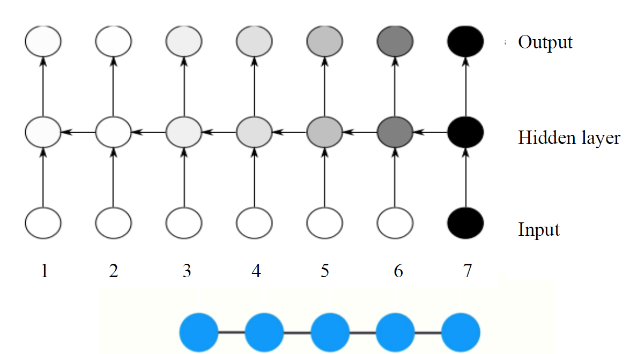
\includegraphics[width=0.55\textwidth]{./appunti_images/media/image11.png}
\caption{Vanishing e exploding gradient nelle RNN: il gradiente si degrada lungo la sequenza temporale.}
\end{figure}

L'\textbf{exploding gradient} si può mitigare con il \textbf{gradient clipping}: se la norma del gradiente supera una soglia $\tau$, si riscala:
\begin{formulabox}[title={\textbf{Gradient Clipping}}]
\[
\mathbf{g} \leftarrow \frac{\tau}{\|\mathbf{g}\|} \cdot \mathbf{g} \quad \text{se } \|\mathbf{g}\| > \tau
\]
\end{formulabox}

Il vanishing gradient è invece più insidioso. Nella pratica, le RNN standard riescono a catturare dipendenze solo fino a circa 10 passi temporali. Per sequenze lunghe servono architetture con gate espliciti: LSTM e GRU.

% ---------------------------------------------------------------------------

\section{LSTM (Long Short-Term Memory)}
\label{app:lstm}

Le \textbf{LSTM}, introdotte da \textbf{Hochreiter \& Schmidhuber (1997)} in ``Long Short-Term Memory'' (Neural Computation), risolvono il vanishing gradient introducendo una \textbf{cella di memoria} $\mathbf{C}_t$ protetta da tre porte (gate) che controllano il flusso di informazione.

\begin{figure}[htbp]
\centering
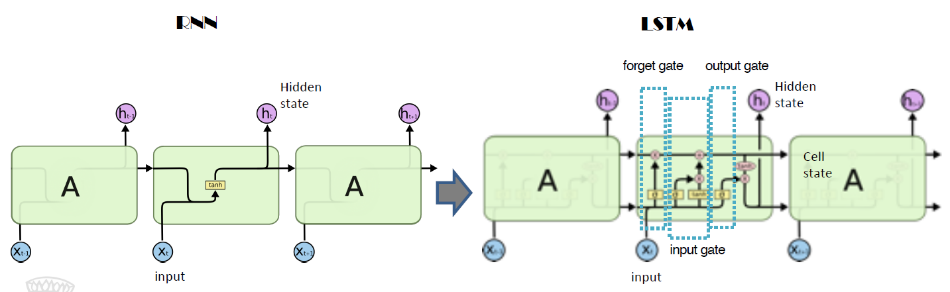
\includegraphics[width=0.55\textwidth]{./appunti_images/media/image12.png}
\caption{Struttura di una cella LSTM con le tre porte (forget, input, output) e la cella di memoria.}
\end{figure}

\needspace{4\baselineskip}
\subsection{Architettura: le 4 equazioni}

\begin{figure}[htbp]
\centering

\includegraphics[width=0.55\textwidth]{./appunti_images/media/image13.png}
\caption{Forget gate della LSTM: $\mathbf{f}_t = \sigma(\mathbf{W}_f[\mathbf{h}_{t-1}, \mathbf{x}_t] + \mathbf{b}_f)$ decide quali informazioni scartare dalla cella.}
\end{figure}

\begin{formulabox}[title={\textbf{Equazioni della LSTM}}]
\begin{align}
\mathbf{f}_t &= \sigma\!\bigl(\mathbf{W}_f\,[\mathbf{h}_{t-1},\,\mathbf{x}_t] + \mathbf{b}_f\bigr) & \text{(Forget gate)} \\[4pt]
\mathbf{i}_t &= \sigma\!\bigl(\mathbf{W}_i\,[\mathbf{h}_{t-1},\,\mathbf{x}_t] + \mathbf{b}_i\bigr) & \text{(Input gate)} \\[4pt]
\mathbf{C}_t &= \mathbf{f}_t \odot \mathbf{C}_{t-1} + \mathbf{i}_t \odot \tanh\!\bigl(\mathbf{W}_C\,[\mathbf{h}_{t-1},\,\mathbf{x}_t] + \mathbf{b}_C\bigr) & \text{(State update)} \\[4pt]
\mathbf{h}_t &= \sigma\!\bigl(\mathbf{W}_o\,[\mathbf{h}_{t-1},\,\mathbf{x}_t] + \mathbf{b}_o\bigr) \odot \tanh(\mathbf{C}_t) & \text{(Output gate)}
\end{align}
\end{formulabox}

\begin{notabox}[title={\textbf{In parole semplici}}]
\begin{itemize}
\item \textbf{Forget gate} ($\mathbf{f}_t$): decide cosa \emph{dimenticare} dalla memoria precedente ($\sigma \approx 0 \to$ dimentica, $\sigma \approx 1 \to$ mantieni).
\item \textbf{Input gate} ($\mathbf{i}_t$): decide cosa \emph{aggiungere} di nuovo alla memoria.
\item \textbf{State update} ($\mathbf{C}_t$): aggiorna la cella combinando il vecchio stato (filtrato) con le nuove informazioni.
\item \textbf{Output gate}: decide quale parte della memoria esporre come output $\mathbf{h}_t$.
\end{itemize}
\end{notabox}

\begin{notabox}[title={\textbf{In parole semplici: LSTM che legge un testo}}]
Immagina una LSTM che legge: ``Il gatto, che era nero e aveva gli occhi verdi, \textbf{corse} via''. La cella di memoria deve ricordare ``il gatto'' (soggetto singolare) attraverso tutta la subordinata. Il \textbf{forget gate} decide di non dimenticare il soggetto. L'\textbf{input gate} aggiunge informazioni sugli aggettivi senza sovrascrivere il soggetto. Quando arriva il verbo, l'\textbf{output gate} produce lo stato nascosto che codifica ``soggetto singolare'', permettendo di concordare correttamente il verbo.
\end{notabox}

\begin{notabox}[title={\textbf{Esempio numerico: forward pass LSTM gate per gate}}]
LSTM con $d_h = 2$, $d_x = 1$. Stato iniziale: $\mathbf{h}_{t-1} = (0.2,\, -0.1)^\top$, $\mathbf{C}_{t-1} = (0.5,\, 0.3)^\top$, input $x_t = 0.7$. Vettore concatenato: $[\mathbf{h}_{t-1}, x_t] = (0.2,\; -0.1,\; 0.7)$.

\textbf{Passo 1 --- Forget Gate.} $\mathbf{f}_t = \sigma(0.69,\, 0.41)^\top = (0.666,\, 0.601)^\top$ --- mantiene buona parte della cella.

\textbf{Passo 2 --- Input Gate.} $\mathbf{i}_t = \sigma(0.28,\, 0.23)^\top = (0.570,\, 0.557)^\top$.

\textbf{Passo 3 --- Candidato.} $\tilde{\mathbf{C}}_t = \tanh(0.47,\, -0.15)^\top = (0.438,\, -0.149)^\top$.

\textbf{Passo 4 --- Aggiornamento della cella:}
$\mathbf{C}_t = \mathbf{f}_t \odot \mathbf{C}_{t-1} + \mathbf{i}_t \odot \tilde{\mathbf{C}}_t = (0.583,\, 0.097)^\top$.

\textbf{Passo 5 --- Output Gate:} $\mathbf{o}_t = \sigma(0.26,\, -0.01)^\top = (0.565,\, 0.498)^\top$. $\mathbf{h}_t = \mathbf{o}_t \odot \tanh(\mathbf{C}_t) = (0.296,\, 0.048)^\top$.

\textbf{Interpretazione:} la cella ha mantenuto buona parte della prima componente ($0.5 \to 0.583$) ma la seconda è scesa ($0.3 \to 0.097$). Lo stato nascosto è una versione ``filtrata'' della cella.
\end{notabox}

\begin{figure}[htbp]
\centering

\includegraphics[width=0.50\textwidth]{./appunti_images/media/image14.png}
\hfill

\includegraphics[width=0.50\textwidth]{./appunti_images/media/image15.png}
\caption{Sinistra: input gate e candidato ($i_t$, $\tilde{C}_t$). Destra: aggiornamento della cella di memoria ($C_t = f_t \odot C_{t-1} + i_t \odot \tilde{C}_t$).}
\end{figure}

\begin{figure}[htbp]
\centering

\includegraphics[width=0.55\textwidth]{./appunti_images/media/image16.png}
\caption{Output gate della LSTM: $\mathbf{o}_t = \sigma(\mathbf{W}_o[\mathbf{h}_{t-1}, \mathbf{x}_t] + \mathbf{b}_o)$ e stato nascosto $\mathbf{h}_t = \mathbf{o}_t \odot \tanh(\mathbf{C}_t)$.}
\end{figure}

\begin{notabox}[title={\textbf{Collegamento al Perceiver}}]
La cella $\mathbf{C}_t$ funziona come un ``nastro trasportatore'' che trasporta informazione lungo la sequenza senza degradarla --- la stessa intuizione delle \textbf{residual connections}, che nel Perceiver sono presenti in ogni blocco di attention (112 in totale).
\end{notabox}

Le LSTM funzionano bene ma hanno molti parametri. Una versione semplificata con prestazioni comparabili è la GRU.

% ---------------------------------------------------------------------------

\section{GRU (Gated Recurrent Unit)}

La \textbf{GRU}, introdotta da \textbf{Cho et al.\ (2014)} in ``Learning Phrase Representations using RNN Encoder-Decoder for Statistical Machine Translation'' (EMNLP), semplifica la LSTM fondendo cella e stato nascosto e usando solo \textbf{2 porte} invece di 3.

\begin{figure}[htbp]
\centering
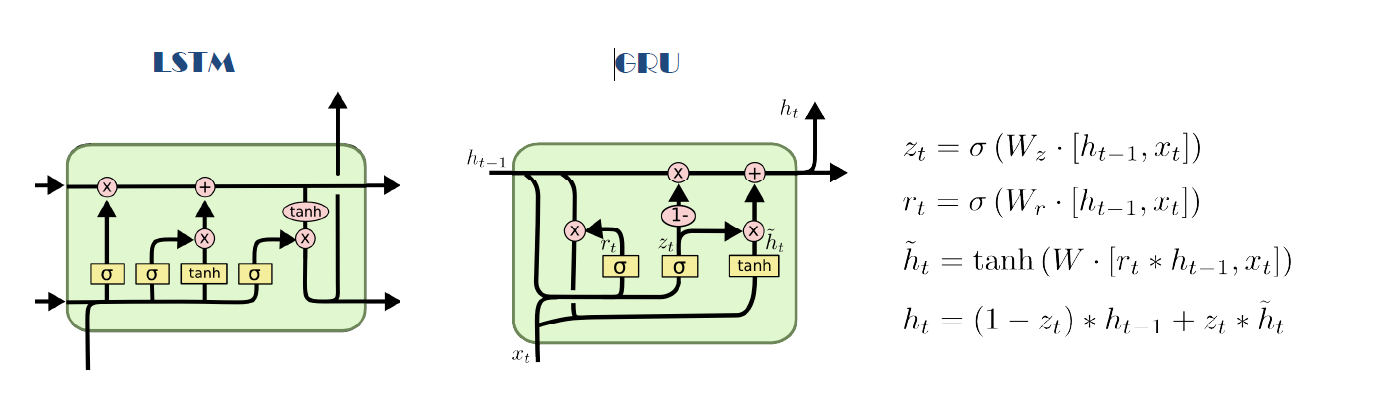
\includegraphics[width=0.55\textwidth]{./appunti_images/media/image17.png}
\caption{Confronto tra LSTM (sinistra) e GRU (destra): la GRU semplifica la struttura fondendo cella e stato nascosto e usando 2 porte invece di 3.}
\end{figure}

\begin{formulabox}[title={\textbf{Equazioni della GRU}}]
\begin{align}
\mathbf{r}_t &= \sigma\!\bigl(\mathbf{W}_r\,[\mathbf{h}_{t-1},\,\mathbf{x}_t] + \mathbf{b}_r\bigr) & \text{(Reset gate)} \\[4pt]
\mathbf{z}_t &= \sigma\!\bigl(\mathbf{W}_z\,[\mathbf{h}_{t-1},\,\mathbf{x}_t] + \mathbf{b}_z\bigr) & \text{(Update gate)} \\[4pt]
\tilde{\mathbf{h}}_t &= \tanh\!\bigl(\mathbf{W}\,[\mathbf{r}_t \odot \mathbf{h}_{t-1},\,\mathbf{x}_t] + \mathbf{b}\bigr) & \text{(Candidato)} \\[4pt]
\mathbf{h}_t &= (1 - \mathbf{z}_t) \odot \mathbf{h}_{t-1} + \mathbf{z}_t \odot \tilde{\mathbf{h}}_t & \text{(Stato aggiornato)}
\end{align}
\end{formulabox}

\begin{notabox}[title={\textbf{Esempio numerico: forward pass di una GRU}}]
GRU con $d_h = 2$, $d_x = 1$. Stato: $\mathbf{h}_{t-1} = (0.5,\, -0.3)^\top$, input $x_t = 0.8$. Concatenato: $(0.5,\; -0.3,\; 0.8)$.

\textbf{Reset Gate:} $\mathbf{r}_t = \sigma(0.41,\, 0.33)^\top = (0.601,\, 0.582)^\top$.
\textbf{Update Gate:} $\mathbf{z}_t = \sigma(0.21,\, -0.15)^\top = (0.552,\, 0.463)^\top$.
\textbf{Candidato:} $\mathbf{r}_t \odot \mathbf{h}_{t-1} = (0.301,\, -0.175)^\top$; $\tilde{\mathbf{h}}_t = \tanh(0.605,\, -0.297)^\top = (0.541,\, -0.289)^\top$.
\textbf{Interpolazione:} $\mathbf{h}_t = (1 - \mathbf{z}_t) \odot \mathbf{h}_{t-1} + \mathbf{z}_t \odot \tilde{\mathbf{h}}_t = (0.523,\, -0.295)^\top$.

\textbf{Interpretazione:} $\mathbf{z}_t \approx (0.55, 0.46)$ --- la GRU ``mescola'' circa metà vecchio stato e metà candidato: aggiornamento graduale.
\end{notabox}

\needspace{4\baselineskip}
\subsection{Confronto GRU vs LSTM}

{\def\LTcaptype{none}
\begin{longtable}{@{}p{0.22\linewidth}p{0.35\linewidth}p{0.35\linewidth}@{}}
\toprule
\textbf{Aspetto} & \textbf{LSTM} & \textbf{GRU} \\
\midrule\endhead
\bottomrule\endlastfoot
Porte & 3 (forget, input, output) & 2 (reset, update) \\
Stato interno & $\mathbf{C}_t$ e $\mathbf{h}_t$ separati & Solo $\mathbf{h}_t$ \\
Parametri & Pi\`u numerosi & $\sim$25\% in meno \\
Sequenze molto lunghe & Leggermente migliore & Comparabile \\
Velocit\`a di training & Pi\`u lenta & Pi\`u veloce \\
\end{longtable}
}

Mentre le RNN (e le loro varianti LSTM/GRU) eccellono con dati sequenziali, per dati strutturati in forma di griglia --- come le \textbf{immagini} --- servono architetture in grado di sfruttare la struttura spaziale locale. Le reti neurali convoluzionali sono state progettate esattamente per questo scopo.

% ---------------------------------------------------------------------------

\section{Reti Neurali Convoluzionali (CNN)}
\label{app:cnn}

Le \textbf{CNN} sono progettate per elaborare dati strutturati a griglia (immagini, video). Invece di connettere ogni neurone a tutti gli input, usano \textbf{filtri locali} (kernel) che scorrono sull'immagine per estrarre feature. Sono il predecessore diretto del ViT e, indirettamente, del Perceiver.

\begin{figure}[htbp]
\centering
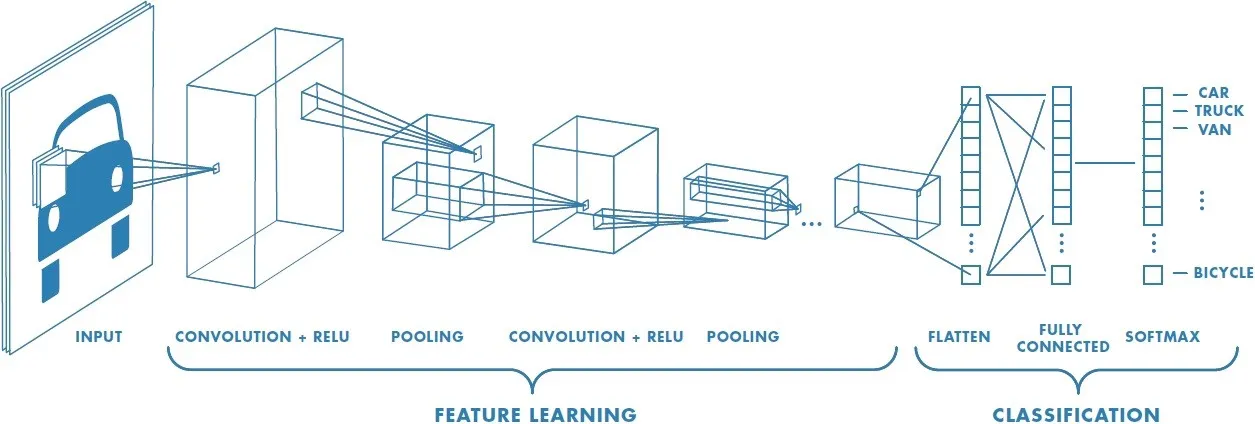
\includegraphics[width=0.60\textwidth]{./appunti_images/media/image18.png}
\caption{Architettura tipica di una CNN: convoluzioni, pooling e fully connected layer.}
\end{figure}

\needspace{4\baselineskip}
\subsection{Architettura overview}

Una CNN tipica alterna tre tipi di layer:
\begin{enumerate}
\item \textbf{Convolution Layer} --- estrae feature locali tramite filtri (kernel)
\item \textbf{Pooling Layer} --- riduce la dimensione spaziale mantenendo le feature pi\`u importanti
\item \textbf{Fully Connected Layer} --- classifica le feature estratte
\end{enumerate}

I Convolution Layer iniziali catturano feature di basso livello (bordi, texture); quelli profondi catturano feature complesse (volti, oggetti).

\needspace{4\baselineskip}
\subsection{Convolution Layer}

Un filtro (kernel) è una piccola matrice di pesi che \textbf{scorre sistematicamente} sull'immagine. In ogni posizione compie tre operazioni in sequenza: (1)~moltiplica ogni suo valore per il pixel corrispondente, (2)~somma tutti i prodotti, (3)~scrive il risultato in una cella della \textbf{feature map}. Poi si sposta e ricomincia.

La cosa da visualizzare è questa: il kernel è un \textbf{rilevatore riutilizzato}. Non impara un peso diverso per ogni pixel dell'immagine; impara un piccolo pattern e lo prova in tutte le posizioni. È qui che nascono insieme \emph{efficienza} (pochi pesi condivisi) e \emph{località} (ogni risposta dipende solo da una piccola regione).

\begin{notabox}[title={\textbf{Convoluzione vs cross-correlation}}]
La \emph{convoluzione matematica} richiederebbe di ruotare il kernel di $180°$ prima di applicarlo. Le CNN reali (PyTorch, TensorFlow, Keras) \textbf{non ruotano il kernel}: eseguono in realtà una \textbf{cross-correlation}. Poiché i pesi vengono comunque appresi, la distinzione non cambia il risultato pratico, ma tecnicamente tutto ciò che chiamiamo ``convoluzione'' nel deep learning è una cross-correlation.
\end{notabox}

\medskip
\textbf{Cosa rappresentano i numeri?}\quad Un'immagine in scala di grigi è una matrice di interi da $0$ (nero) a $255$ (bianco): ogni cella corrisponde a \textbf{un pixel}. Un'immagine $5\times5$ è letteralmente una griglia di 25 valori di intensità luminosa.

Esempio reale: immagine $5\times5$ con una zona chiara a sinistra e una zona nera a destra, separata da un bordo verticale.
\[
X =
\begin{bmatrix}
200 & 200 & 200 & 0 & 0 \\
200 & 200 & 200 & 0 & 0 \\
200 & 200 & 200 & 0 & 0 \\
200 & 200 & 200 & 0 & 0 \\
200 & 200 & 200 & 0 & 0
\end{bmatrix}
\qquad \text{200 = grigio chiaro;\quad 0 = nero}
\]
Scorrendo il kernel di un pixel alla volta (\textbf{stride}~$= 1$, cioè lo spostamento tra una posizione e la successiva) e senza aggiungere bordi artificiali attorno all'immagine (\textbf{padding}~$= 0$), il kernel $3\times3$ può occupare $3\times3 = 9$ posizioni distinte, producendo una feature map $3\times3$. Stride e padding verranno approfonditi più avanti.

\medskip
\textit{Visualizzazione dello scorrimento — il riquadro colorato indica la zona $3\times3$ che il kernel sta esaminando:}

\begin{center}
\begin{tikzpicture}[
  s/.style={draw=gray!35, fill=white,        minimum size=0.47cm, font=\scriptsize,        inner sep=0pt},
  h/.style={draw=seccolor, fill=seccolor!22, minimum size=0.47cm, font=\scriptsize\bfseries, inner sep=0pt, line width=1pt}
]
% ---- reusable shorthand ----
\def\cs{0.47} % cell step

% ===== GRID A  (kernel cols 0-2, righe 0-2) =====
\node[h] at (\cs*0,-\cs*0){200};\node[h] at (\cs*1,-\cs*0){200};\node[h] at (\cs*2,-\cs*0){200};\node[s] at (\cs*3,-\cs*0){0};\node[s] at (\cs*4,-\cs*0){0};
\node[h] at (\cs*0,-\cs*1){200};\node[h] at (\cs*1,-\cs*1){200};\node[h] at (\cs*2,-\cs*1){200};\node[s] at (\cs*3,-\cs*1){0};\node[s] at (\cs*4,-\cs*1){0};
\node[h] at (\cs*0,-\cs*2){200};\node[h] at (\cs*1,-\cs*2){200};\node[h] at (\cs*2,-\cs*2){200};\node[s] at (\cs*3,-\cs*2){0};\node[s] at (\cs*4,-\cs*2){0};
\node[s] at (\cs*0,-\cs*3){200};\node[s] at (\cs*1,-\cs*3){200};\node[s] at (\cs*2,-\cs*3){200};\node[s] at (\cs*3,-\cs*3){0};\node[s] at (\cs*4,-\cs*3){0};
\node[s] at (\cs*0,-\cs*4){200};\node[s] at (\cs*1,-\cs*4){200};\node[s] at (\cs*2,-\cs*4){200};\node[s] at (\cs*3,-\cs*4){0};\node[s] at (\cs*4,-\cs*4){0};
\node[font=\small\bfseries,color=seccolor]    at (\cs*2,-\cs*5.3) {A};
\node[font=\scriptsize,color=gray!70!black] at (\cs*2,-\cs*6.1) {out\,$=$\,$0$};

% arrow A -> B
\draw[->,thick,color=gray!55] (\cs*4.7,-\cs*2) -- (\cs*5.3,-\cs*2);
\node[font=\tiny,color=gray!70] at (\cs*5,-\cs*1.3) {$+1$\,col};

% ===== GRID B  (kernel cols 1-3, righe 0-2) =====
\begin{scope}[xshift=3.4cm]
\node[s] at (\cs*0,-\cs*0){200};\node[h] at (\cs*1,-\cs*0){200};\node[h] at (\cs*2,-\cs*0){200};\node[h] at (\cs*3,-\cs*0){0};\node[s] at (\cs*4,-\cs*0){0};
\node[s] at (\cs*0,-\cs*1){200};\node[h] at (\cs*1,-\cs*1){200};\node[h] at (\cs*2,-\cs*1){200};\node[h] at (\cs*3,-\cs*1){0};\node[s] at (\cs*4,-\cs*1){0};
\node[s] at (\cs*0,-\cs*2){200};\node[h] at (\cs*1,-\cs*2){200};\node[h] at (\cs*2,-\cs*2){200};\node[h] at (\cs*3,-\cs*2){0};\node[s] at (\cs*4,-\cs*2){0};
\node[s] at (\cs*0,-\cs*3){200};\node[s] at (\cs*1,-\cs*3){200};\node[s] at (\cs*2,-\cs*3){200};\node[s] at (\cs*3,-\cs*3){0};\node[s] at (\cs*4,-\cs*3){0};
\node[s] at (\cs*0,-\cs*4){200};\node[s] at (\cs*1,-\cs*4){200};\node[s] at (\cs*2,-\cs*4){200};\node[s] at (\cs*3,-\cs*4){0};\node[s] at (\cs*4,-\cs*4){0};
\node[font=\small\bfseries,color=red!70!black]  at (\cs*2,-\cs*5.3) {B};
\node[font=\scriptsize\bfseries,color=red!70!black] at (\cs*2,-\cs*6.1) {out\,$=$\,$600$};
\end{scope}

% arrow B -> C
\draw[->,thick,color=gray!55] (3.4cm+\cs*4.7,-\cs*2) -- (3.4cm+\cs*5.3,-\cs*2);
\node[font=\tiny,color=gray!70] at (3.4cm+\cs*5,-\cs*1.3) {$+1$\,col};

% ===== GRID C  (kernel cols 2-4, righe 0-2) =====
\begin{scope}[xshift=6.8cm]
\node[s] at (\cs*0,-\cs*0){200};\node[s] at (\cs*1,-\cs*0){200};\node[h] at (\cs*2,-\cs*0){200};\node[h] at (\cs*3,-\cs*0){0};\node[h] at (\cs*4,-\cs*0){0};
\node[s] at (\cs*0,-\cs*1){200};\node[s] at (\cs*1,-\cs*1){200};\node[h] at (\cs*2,-\cs*1){200};\node[h] at (\cs*3,-\cs*1){0};\node[h] at (\cs*4,-\cs*1){0};
\node[s] at (\cs*0,-\cs*2){200};\node[s] at (\cs*1,-\cs*2){200};\node[h] at (\cs*2,-\cs*2){200};\node[h] at (\cs*3,-\cs*2){0};\node[h] at (\cs*4,-\cs*2){0};
\node[s] at (\cs*0,-\cs*3){200};\node[s] at (\cs*1,-\cs*3){200};\node[s] at (\cs*2,-\cs*3){200};\node[s] at (\cs*3,-\cs*3){0};\node[s] at (\cs*4,-\cs*3){0};
\node[s] at (\cs*0,-\cs*4){200};\node[s] at (\cs*1,-\cs*4){200};\node[s] at (\cs*2,-\cs*4){200};\node[s] at (\cs*3,-\cs*4){0};\node[s] at (\cs*4,-\cs*4){0};
\node[font=\small\bfseries,color=red!70!black]  at (\cs*2,-\cs*5.3) {C};
\node[font=\scriptsize\bfseries,color=red!70!black] at (\cs*2,-\cs*6.1) {out\,$=$\,$600$};
\end{scope}

% big arrow -> feature map
\draw[->,very thick,color=seccolor!65] (9.05,-\cs*2.5) -- (9.55,-\cs*2.5);
\node[font=\footnotesize\bfseries,color=seccolor,align=center] at (9.3,-\cs*0.8) {feature\\map};

% ===== FEATURE MAP  (3x3) =====
\def\fm{0.60} % feature-map cell step
\begin{scope}[xshift=9.75cm]
\node[draw=gray!40,fill=gray!10, minimum width=\fm cm,minimum height=0.50cm,font=\scriptsize,inner sep=0pt] at (\fm*0,-\fm*0){0};
\node[draw=gray!40,fill=red!22, minimum width=\fm cm,minimum height=0.50cm,font=\scriptsize\bfseries,inner sep=0pt] at (\fm*1,-\fm*0){600};
\node[draw=gray!40,fill=red!22, minimum width=\fm cm,minimum height=0.50cm,font=\scriptsize\bfseries,inner sep=0pt] at (\fm*2,-\fm*0){600};
\node[draw=gray!40,fill=gray!10, minimum width=\fm cm,minimum height=0.50cm,font=\scriptsize,inner sep=0pt] at (\fm*0,-\fm*1){0};
\node[draw=gray!40,fill=red!22, minimum width=\fm cm,minimum height=0.50cm,font=\scriptsize\bfseries,inner sep=0pt] at (\fm*1,-\fm*1){600};
\node[draw=gray!40,fill=red!22, minimum width=\fm cm,minimum height=0.50cm,font=\scriptsize\bfseries,inner sep=0pt] at (\fm*2,-\fm*1){600};
\node[draw=gray!40,fill=gray!10, minimum width=\fm cm,minimum height=0.50cm,font=\scriptsize,inner sep=0pt] at (\fm*0,-\fm*2){0};
\node[draw=gray!40,fill=red!22, minimum width=\fm cm,minimum height=0.50cm,font=\scriptsize\bfseries,inner sep=0pt] at (\fm*1,-\fm*2){600};
\node[draw=gray!40,fill=red!22, minimum width=\fm cm,minimum height=0.50cm,font=\scriptsize\bfseries,inner sep=0pt] at (\fm*2,-\fm*2){600};
\node[font=\footnotesize\bfseries,color=seccolor] at (\fm*1,-\cs*5.3) {Feature Map};
\end{scope}

\end{tikzpicture}
\end{center}

\begin{formulabox}[title={\textbf{Come funziona il kernel: passo per passo}}]
\textbf{Posizione A — kernel su zona uniforme (colonne 0–2, tutte a 200):}
\[
\underbrace{\begin{bmatrix}1&0&{-1}\\1&0&{-1}\\1&0&{-1}\end{bmatrix}}_{\text{kernel}}
\;\text{su}\;
\underbrace{\begin{bmatrix}200&200&200\\200&200&200\\200&200&200\end{bmatrix}}_{\text{zona A}}
\]
\[
(1\!\cdot\!200)+(0\!\cdot\!200)+(-1\!\cdot\!200)
\;+\;
(\ldots)\;+\;(\ldots)
\;=\; 0+0+0 = \mathbf{0}
\]
\textit{Luminosità uniforme: i contributi si annullano. Nessun bordo.}

\medskip
\textbf{Posizione B — kernel sul bordo (colonne 1–3, transizione 200$\to$0):}
\[
\underbrace{\begin{bmatrix}1&0&{-1}\\1&0&{-1}\\1&0&{-1}\end{bmatrix}}_{\text{kernel}}
\;\text{su}\;
\underbrace{\begin{bmatrix}200&200&0\\200&200&0\\200&200&0\end{bmatrix}}_{\text{zona B}}
\]
\[
\underbrace{(1\!\cdot\!200)}_{200}+\underbrace{(0\!\cdot\!200)}_{0}+\underbrace{(-1\!\cdot\!0)}_{0}
\;+\;
\underbrace{(1\!\cdot\!200)}_{200}+\underbrace{(0\!\cdot\!200)}_{0}+\underbrace{(-1\!\cdot\!0)}_{0}
\;+\;
\underbrace{(1\!\cdot\!200)}_{200}+\underbrace{(0\!\cdot\!200)}_{0}+\underbrace{(-1\!\cdot\!0)}_{0}
= \mathbf{600}
\]
\textit{Sinistra luminosa (200), destra nera (0): differenza massima. Bordo rilevato!}

\medskip
\textbf{Feature map completa} (dopo aver scansionato tutta l'immagine con stride~1):
\[
\text{feature map} =
\begin{bmatrix}
0 & 600 & 600 \\
0 & 600 & 600 \\
0 & 600 & 600
\end{bmatrix}
\]
I valori alti (600) segnalano la presenza del bordo verticale in quella posizione. In forma compatta: $\displaystyle\sum_{i,j} K_{ij}\cdot X_{ij}$.
\end{formulabox}

\medskip
\textbf{Perché questo filtro rileva bordi verticali?}
Il kernel ha pesi $+1$ a sinistra e $-1$ a destra. Dove la sinistra è luminosa e la destra è scura, la differenza è grande $\Rightarrow$ output alto. Dove la luminosità è uniforme, i contributi positivi e negativi si annullano $\Rightarrow$ output vicino a zero. Il filtro misura quindi una \emph{transizione laterale di luminosità}, cioè un bordo verticale.

\begin{formulabox}[title={\textbf{Feature map}}]
La feature map è la matrice di output che raccoglie tutti i risultati:
\[
\text{feature map}(i,j) = \sum_{m,n} K_{mn}\cdot X_{i+m,\,j+n}
\]
\begin{tabular}{ll}
$i,j$ & posizione corrente del kernel nell'immagine di output \\
$m,n$ & coordinate interne al kernel (da $0$ a $k-1$) \\
\end{tabular}\\[4pt]
Ogni cella dice \textbf{quanto} il pattern cercato dal filtro è presente in quella posizione. Valore alto~$=$~pattern trovato; valore basso (o zero dopo ReLU)~$=$~pattern assente.
\end{formulabox}

\medskip
\textbf{Bias.}\quad In pratica, al risultato della convoluzione viene aggiunto un \textbf{bias apprendibile} $b$: $\text{output} = (K \ast X) + b$. Il bias consente al filtro di traslare la soglia di attivazione indipendentemente dall'input, aumentando l'espressività del modello.

\medskip
\textbf{Perché ReLU?}\quad Dopo la convoluzione si applica $\text{ReLU}(x)=\max(0,x)$, che azzera i valori negativi e mantiene quelli positivi. Senza attivazione non lineare, componendo solo operazioni lineari, l'intera rete sarebbe equivalente a una singola trasformazione lineare e non potrebbe imparare pattern complessi.

\begin{formulabox}[title={\textbf{Esempio ReLU}}]
Input: $[-5,\;2,\;7,\;-1]$\quad$\xrightarrow{\;\text{ReLU}\;}$\quad Output: $[0,\;2,\;7,\;0]$
\end{formulabox}

\medskip
\textbf{Stride e Padding.}\quad
Lo \textbf{stride} $s$ indica di quanti pixel si sposta il kernel a ogni passo:
\begin{itemize}
  \item $s=1$: si sposta di un pixel, output grande, molti dettagli.
  \item $s=2$: salta un pixel, output più piccolo, meno calcoli.
\end{itemize}
Il \textbf{padding} $p$ aggiunge un bordo di zeri attorno all'immagine. Senza padding l'immagine si restringe dopo ogni convoluzione; con padding si mantengono le dimensioni originali.

\begin{formulabox}[title={\textbf{Dimensione dell'output}}]
Data un'immagine $H \times W$, filtro $k\times k$, stride $s$, padding $p$:
\[
H_{\text{out}} = \left\lfloor\frac{H - k + 2p}{s}\right\rfloor + 1
\qquad
W_{\text{out}} = \left\lfloor\frac{W - k + 2p}{s}\right\rfloor + 1
\]
\textit{Lettura:} il numeratore è lo spazio disponibile dopo padding e rimozione del kernel; dividendo per $s$ si ottiene quante posizioni può visitare; il $+1$ aggiunge la posizione iniziale.
\end{formulabox}

\begin{notabox}[title={\textbf{I filtri vengono appresi, non scritti a mano}}]
Nelle CNN reali i kernel \textbf{non sono progettati manualmente}. All'inizio hanno pesi casuali; durante il training la backpropagation li aggiorna automaticamente. La rete impara:
\begin{itemize}
  \item nei primi layer: bordi, gradienti di colore, texture semplici;
  \item nei layer intermedi: forme geometriche, pattern ricorrenti;
  \item nei layer profondi: parti di oggetti, volti, strutture complesse.
\end{itemize}
È questo apprendimento gerarchico che rende le CNN così potenti.
\end{notabox}

\medskip
\textbf{Immagini a colori (RGB).}\quad Un'immagine reale ha 3 canali (R, G, B). Il kernel non è $k{\times}k$ ma $k{\times}k{\times}3$: opera su tutti e tre i canali simultaneamente. Ogni filtro combina i tre canali e produce \textbf{una feature map completa}. Con $F$ filtri si ottengono $F$ feature map in output — una per ogni pattern cercato.

\begin{formulabox}[title={\textbf{Pipeline completa di una CNN}}]
\begin{gather*}
\text{Input}
\xrightarrow{\text{Conv+bias}}
\text{Feature map}
\xrightarrow{\text{ReLU}}
\text{Attivazione}
\xrightarrow{\text{Pooling}}
\text{Ridotta}
\xrightarrow{\text{Conv+ReLU+Pool}\;\cdots} \\[6pt]
\cdots\xrightarrow{\text{Flatten}}
\text{Vettore 1D}
\xrightarrow{\text{FC}}
\text{Logit}
\xrightarrow{\text{Softmax}}
\text{Output}
\end{gather*}
I blocchi Conv+ReLU+Pool si ripetono più volte (layer profondi = feature più astratte); il Flatten porta a uno o più layer Fully Connected per la classificazione finale.
\end{formulabox}

\needspace{4\baselineskip}
\subsection{Pooling}

Il pooling riduce la dimensione spaziale della feature map mantenendo le informazioni più rilevanti. Serve a tre scopi: (1)~diminuire il costo computazionale, (2)~ridurre l'overfitting, (3)~rendere la rete meno sensibile alla posizione esatta dei pattern.

\textbf{Max-pooling.}\quad Divide la feature map in finestre non sovrapposte e prende il valore massimo di ciascuna. Con finestra $2\times2$ e stride~2, ogni quadrante si riduce a un singolo valore:

\[
\begin{bmatrix}
1 & 2 & 3 & 4 \\
5 & \mathbf{6} & 7 & \mathbf{8} \\
9 & 10 & 11 & 12 \\
13 & \mathbf{14} & 15 & \mathbf{16}
\end{bmatrix}
\xrightarrow{\text{Max-Pool } 2\!\times\!2}
\begin{bmatrix}
6 & 8 \\
14 & 16
\end{bmatrix}
\]

Il massimo cattura \emph{se} il pattern è presente nella finestra, indipendentemente da dove si trova esattamente. Per questo le CNN sono robuste a piccole traslazioni dell'input.

\textbf{Average-pooling.}\quad Prende la media invece del massimo: conserva informazioni diffuse su tutta la finestra. Utile negli strati finali di alcune architetture (es.\ Global Average Pooling che comprime ogni feature map a un solo valore).

\begin{formulabox}[title={\textbf{Dimensione dopo pooling}}]
Con finestra $p\times p$ e stride $s$:
\[
H_{\text{out}} = \left\lfloor\frac{H - p}{s}\right\rfloor + 1
\]
Esempio: feature map $28\times28$ con Max-Pool $2\times2$ stride~2 $\;\Rightarrow\;$ output $14\times14$.
\end{formulabox}

\begin{figure}[htbp]
\centering
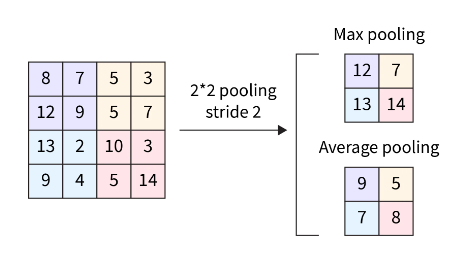
\includegraphics[width=0.50\textwidth]{./appunti_images/media/image22.png}
\caption{Max pooling e Average pooling a confronto.}
\end{figure}

\begin{notabox}[title={\textbf{Attenzione: il pooling è irreversibile}}]
Il pooling è utile perché riduce costo e dimensioni, ma è anche \textbf{irreversibile}: una volta tenuto solo il massimo (o la media) di ogni finestra, i dettagli scartati non sono più recuperabili. È un compromesso voluto --- si rinuncia alla posizione esatta in cambio di robustezza e compattezza.
\end{notabox}

\needspace{4\baselineskip}
\subsection{Fully Connected e Output}

Dopo gli strati convoluzionali le feature map vengono \textbf{appiattite} (flatten) in un unico vettore 1D. Esempio: 32~feature map di dimensione $7\times7$ diventano un vettore di $32\times7\times7 = 1\,568$ valori. Questo vettore riassume tutto ciò che la rete ha rilevato nell'immagine.

\begin{formulabox}[title={\textbf{Layer Fully Connected}}]
Il layer FC calcola:
\[
\mathbf{z} = W\mathbf{x} + \mathbf{b}
\]
dove $\mathbf{x}$ è il vettore appiattito, $W$ la matrice dei pesi e $\mathbf{b}$ il bias. Ogni neurone di output è connesso a \emph{tutti} i valori del vettore (da qui il nome ``fully connected'').
\end{formulabox}

\textbf{Output finale.}
\begin{itemize}
  \item \textbf{Classificazione multiclasse:} si applica \textbf{softmax}, che converte i logit in probabilità che sommano a 1:
  \[
  \text{softmax}(z_i) = \frac{e^{z_i}}{\displaystyle\sum_j e^{z_j}}
  \]
  Esempio: logit $[2.1,\;0.5,\;1.8]$ $\xrightarrow{\text{softmax}}$ $[0.57,\;0.12,\;0.41]$.\\
  La classe predetta è quella con probabilità più alta.
  \item \textbf{Classificazione binaria:} si applica \textbf{sigmoid}, che mappa l'output in $[0,1]$: $\sigma(z)=1/(1+e^{-z})$.
\end{itemize}

\begin{figure}[htbp]
\centering
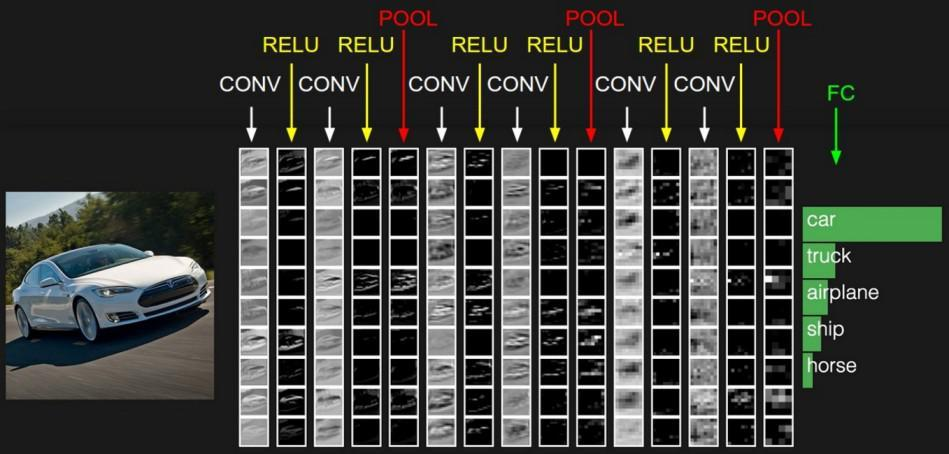
\includegraphics[width=0.55\textwidth]{./appunti_images/media/image23.jpg}
\hfill
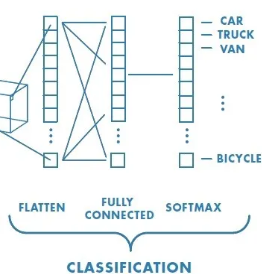
\includegraphics[width=0.30\textwidth]{./appunti_images/media/image24.png}
\caption{Sinistra: visualizzazione delle feature apprese dai filtri convoluzionali (dai bordi alle strutture complesse). Destra: lo stadio di classificazione (Flatten $\to$ FC $\to$ Softmax).}
\end{figure}

\needspace{4\baselineskip}
\subsection{Training}

Il training segue lo stesso ciclo descritto nella Sezione 2 (feed-forward): forward pass $\to$ calcolo della loss $\to$ backpropagation $\to$ aggiornamento dei pesi. La differenza rispetto a un MLP è che i gradienti vengono propagati \emph{anche attraverso i filtri convoluzionali}: sono i pesi dei kernel $K_{ij}$ ad essere aggiornati, non solo quelli dei layer FC.

\begin{formulabox}[title={\textbf{Cosa si aggiorna durante il training}}]
\begin{tabular}{ll}
\textbf{Layer convoluzionale} & pesi del kernel $K_{ij}$ e bias \\
\textbf{Layer FC} & matrice $W$ e bias $\mathbf{b}$ \\
\end{tabular}\\[4pt]
La backprop calcola $\partial\mathcal{L}/\partial K_{ij}$ e aggiorna ogni peso del filtro. Nel tempo la rete impara quali pattern cercare, senza che nessuno li specifichi manualmente.
\end{formulabox}

\begin{notabox}[title={\textbf{In parole semplici: i due inductive bias delle CNN}}]
Le CNN sfruttano due proprietà fondamentali delle immagini:
\begin{enumerate}
\item \textbf{Località:} i pixel vicini sono correlati. Ha senso analizzare l'immagine con filtri piccoli piuttosto che collegare ogni pixel a ogni neurone. Questo riduce drasticamente i parametri.
\item \textbf{Invarianza alla traslazione:} un gatto resta un gatto ovunque nell'immagine. La \emph{condivisione dei pesi} (lo stesso kernel si applica ovunque) garantisce questa proprietà.
\end{enumerate}
Questi inductive bias rendono le CNN efficienti per le immagini, ma le ``imprigionano'': una CNN non sa gestire dati senza struttura a griglia. Il Perceiver rinuncia completamente a entrambi, trattando l'input come una sequenza generica.
\end{notabox}

\begin{notabox}[title={\textbf{Esempio numerico: conteggio parametri di C1 in LeNet-5}}]
Lo strato C1 ha 6 filtri $5 \times 5 \times 1$, ciascuno con un bias:
$\text{Parametri C1} = 6 \times (5 \times 5 \times 1 + 1) = 6 \times 26 = 156$.
Confronto: un MLP fully connected richiederebbe $1\,024 \times 4\,704 \approx 4.8\text{M}$ parametri --- \textbf{30\,000 volte di più}.
\end{notabox}

\medskip
Aumentando la profondità di una CNN, si incorre negli stessi problemi delle RNN: \textbf{vanishing gradient} e \textbf{degradazione delle prestazioni}. La ResNet risolve entrambi con un'idea semplice ma potente.

% ---------------------------------------------------------------------------
\needspace{4\baselineskip}
\subsection{ResNet e Residual Connections}
\label{app:resnet}

\textbf{ResNet} (He et al., 2016) introduce le \textbf{skip connections}: invece di imparare una trasformazione complessa $H(\mathbf{x})$, la rete impara solo la differenza residua $F(\mathbf{x}) = H(\mathbf{x}) - \mathbf{x}$.

\begin{formulabox}[title={\textbf{Residual Connection}}]
\[
\mathbf{y} = F(\mathbf{x}, \mathbf{W}) + \mathbf{x}
\]
\end{formulabox}

\begin{figure}[htbp]
\centering
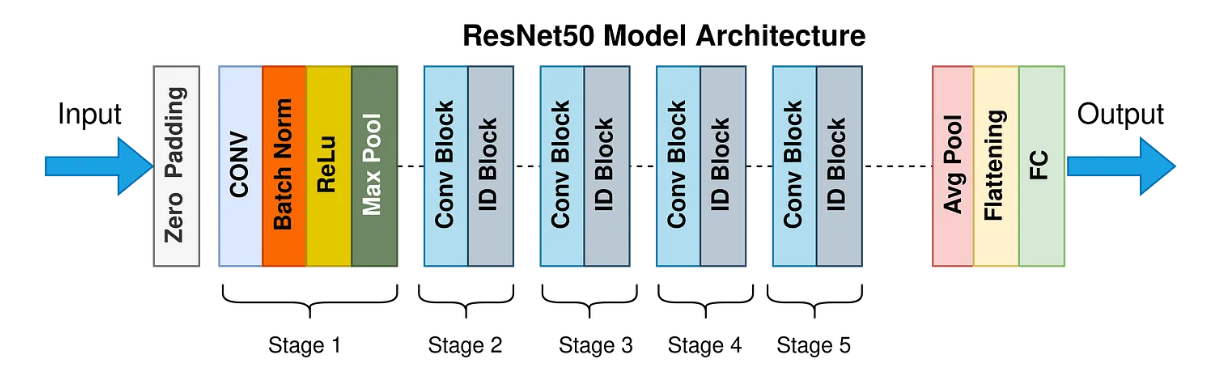
\includegraphics[width=0.60\textwidth]{./appunti_images/media/image25.png}
\caption{Skip connection nella ResNet: il blocco apprende solo il residuo $F(\mathbf{x})$.}
\end{figure}

Perché funziona:
\begin{itemize}
\item Il gradiente può fluire direttamente attraverso la skip connection, evitando il vanishing gradient.
\item Se un layer non è utile, la rete può ``saltarlo'' ($F(\mathbf{x}) \approx 0 \Rightarrow \mathbf{y} \approx \mathbf{x}$).
\item Permette di addestrare reti molto profonde (50, 101, 152+ layer).
\end{itemize}

\begin{figure}[htbp]
\centering
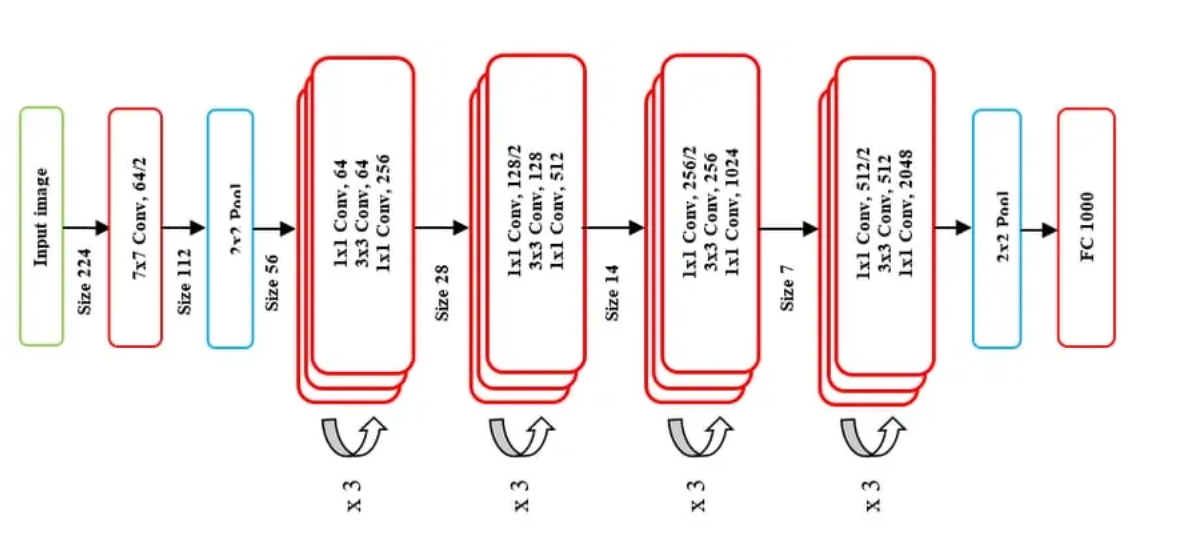
\includegraphics[width=0.55\textwidth]{./appunti_images/media/image26.png}
\caption{Architettura dettagliata di un blocco residuale della ResNet.}
\end{figure}

\begin{notabox}[title={\textbf{Degradazione vs vanishing gradient}}]
Il \textbf{problema della degradazione} è distinto dal vanishing gradient: aggiungere più strati peggiorava le prestazioni \emph{anche sul training set}. Una rete a 56 strati funzionava peggio di una a 20, nonostante contenga la soluzione della rete più bassa. Le skip connections risolvono il problema rendendo l'identità il punto di partenza: il blocco deve apprendere solo $F(\mathbf{x}) \approx 0$.
\end{notabox}

\begin{notabox}[title={\textbf{Bottleneck block (ResNet-50+)}}]
Per reti molto profonde si usa un \textbf{bottleneck block} con tre convoluzioni:
\begin{enumerate}
\item \textbf{Conv} $1 \times 1$ (riduzione): da 256 a 64 canali.
\item \textbf{Conv} $3 \times 3$: operazione convoluzionale nello spazio ridotto.
\item \textbf{Conv} $1 \times 1$ (espansione): da 64 a 256 canali.
\end{enumerate}
Riduce i FLOP di circa $3\times$. Concettualmente simile al \textbf{latent bottleneck del Perceiver}: comprimere, elaborare, ri-espandere.
\end{notabox}

\begin{notabox}[title={\textbf{Collegamento al Perceiver}}]
Il Perceiver usa \textbf{112 residual connections} (una per ogni blocco di attention e FFN). Senza di esse, il training di un modello così profondo sarebbe impossibile.
\end{notabox}

\textbf{Confronto CNN tradizionale vs ResNet-50}

{\def\LTcaptype{none}
\begin{longtable}{@{}
  >{\raggedright\arraybackslash}p{0.20\linewidth}
  >{\raggedright\arraybackslash}p{0.36\linewidth}
  >{\raggedright\arraybackslash}p{0.36\linewidth}@{}}
\toprule
\textbf{Aspetto} & \textbf{CNN tradizionale} & \textbf{ResNet-50} \\
\midrule\endhead
\bottomrule\endlastfoot
Architettura & Sequenziale: Conv $\to$ ReLU $\to$ Pool $\to$ FC & 5 stadi con Residual Blocks + skip connections \\
Flusso info & Solo sequenziale & Doppio: sequenziale + scorciatoia \\
Profondit\`a & 5--19 layer (poi instabile) & 50+ layer, stabile \\
Residual Learning & Assente & $\mathbf{y} = F(\mathbf{x}) + \mathbf{x}$ \\
Vanishing gradient & Presente in reti profonde & Risolto dalle skip connections \\
ImageNet top-5 error & AlexNet 15.3\%, VGG 7.3\% & ResNet-50: 3.57\% \\
\end{longtable}
}

Le CNN (anche con ResNet) catturano pattern \textbf{locali} tramite filtri di dimensione fissa. Per catturare relazioni \textbf{globali} tra tutti gli elementi di una sequenza in un singolo passo, servono i Transformer.

% ---------------------------------------------------------------------------

\section{Transformer}
\label{app:transformer}

Le \hyperref[app:cnn]{CNN} hanno visione locale (limitata al kernel), le \hyperref[app:rnn]{RNN} soffrono di vanishing gradient su sequenze lunghe. Il \textbf{Transformer} (Vaswani et al., 2017, ``Attention Is All You Need'') supera entrambi i limiti con il meccanismo di \textbf{self-attention}, che mette in relazione \emph{ogni} elemento con tutti gli altri in un singolo passo, con complessità $O(M^2)$ dove $M$ è la lunghezza della sequenza.

\needspace{4\baselineskip}
\subsection{Architettura overview}

Il Transformer segue uno schema \textbf{encoder-decoder}:

\begin{figure}[htbp]
\centering
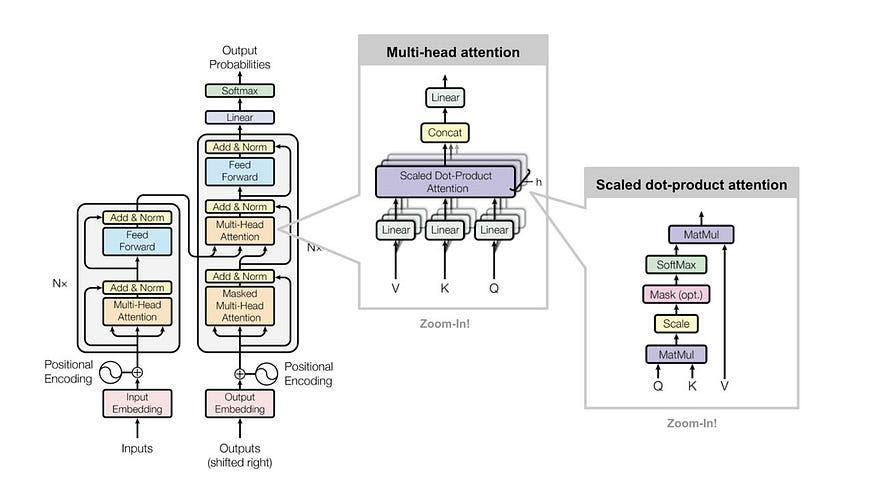
\includegraphics[width=0.55\textwidth]{./appunti_images/media/image27.jpeg}
\caption{Architettura del Transformer: encoder (sinistra) e decoder (destra). Entrambi sono composti da blocchi ripetuti $N\times$ contenenti attention + FFN + residual + LayerNorm.}
\end{figure}

\begin{itemize}
\item \textbf{Encoder}: elabora l'input e produce una rappresentazione contestualizzata. Ogni token ``vede'' tutti gli altri token tramite self-attention.
\item \textbf{Decoder}: genera l'output sequenziale, condizionato dall'encoder. Usa masked self-attention (non può vedere token futuri) e cross-attention (legge dall'encoder).
\item Entrambi usano: input/output embedding + positional encoding.
\end{itemize}

\needspace{4\baselineskip}
\subsection{Input: Tokenizzazione ed Embedding}

Prima di entrare nel Transformer, il testo grezzo viene trasformato in vettori numerici:

\begin{enumerate}
\item \textbf{Tokenizzazione}: il testo viene diviso in unità (token). Metodi comuni: word-level (``gatto'' $\to$ un token), subword (BPE/SentencePiece: ``giocando'' $\to$ ``gioc'' + ``ando''), byte-level (usato nel Perceiver IO).
\item \textbf{Embedding}: ogni token viene mappato in un vettore denso tramite una tabella appresa $E \in \mathbb{R}^{|\text{vocab}| \times d}$, dove $d$ è la dimensione del modello (es. $d = 512$ nel Transformer originale).
\item \textbf{Positional Encoding}: viene sommato all'embedding per fornire informazione sulla posizione (vedi sotto).
\end{enumerate}

\[
\mathbf{z}_i = \text{Embed}(\text{token}_i) + \text{PE}(i) \quad \in \mathbb{R}^{d}
\]

\needspace{4\baselineskip}
\subsection{Encoder}

\begin{figure}[htbp]
\centering
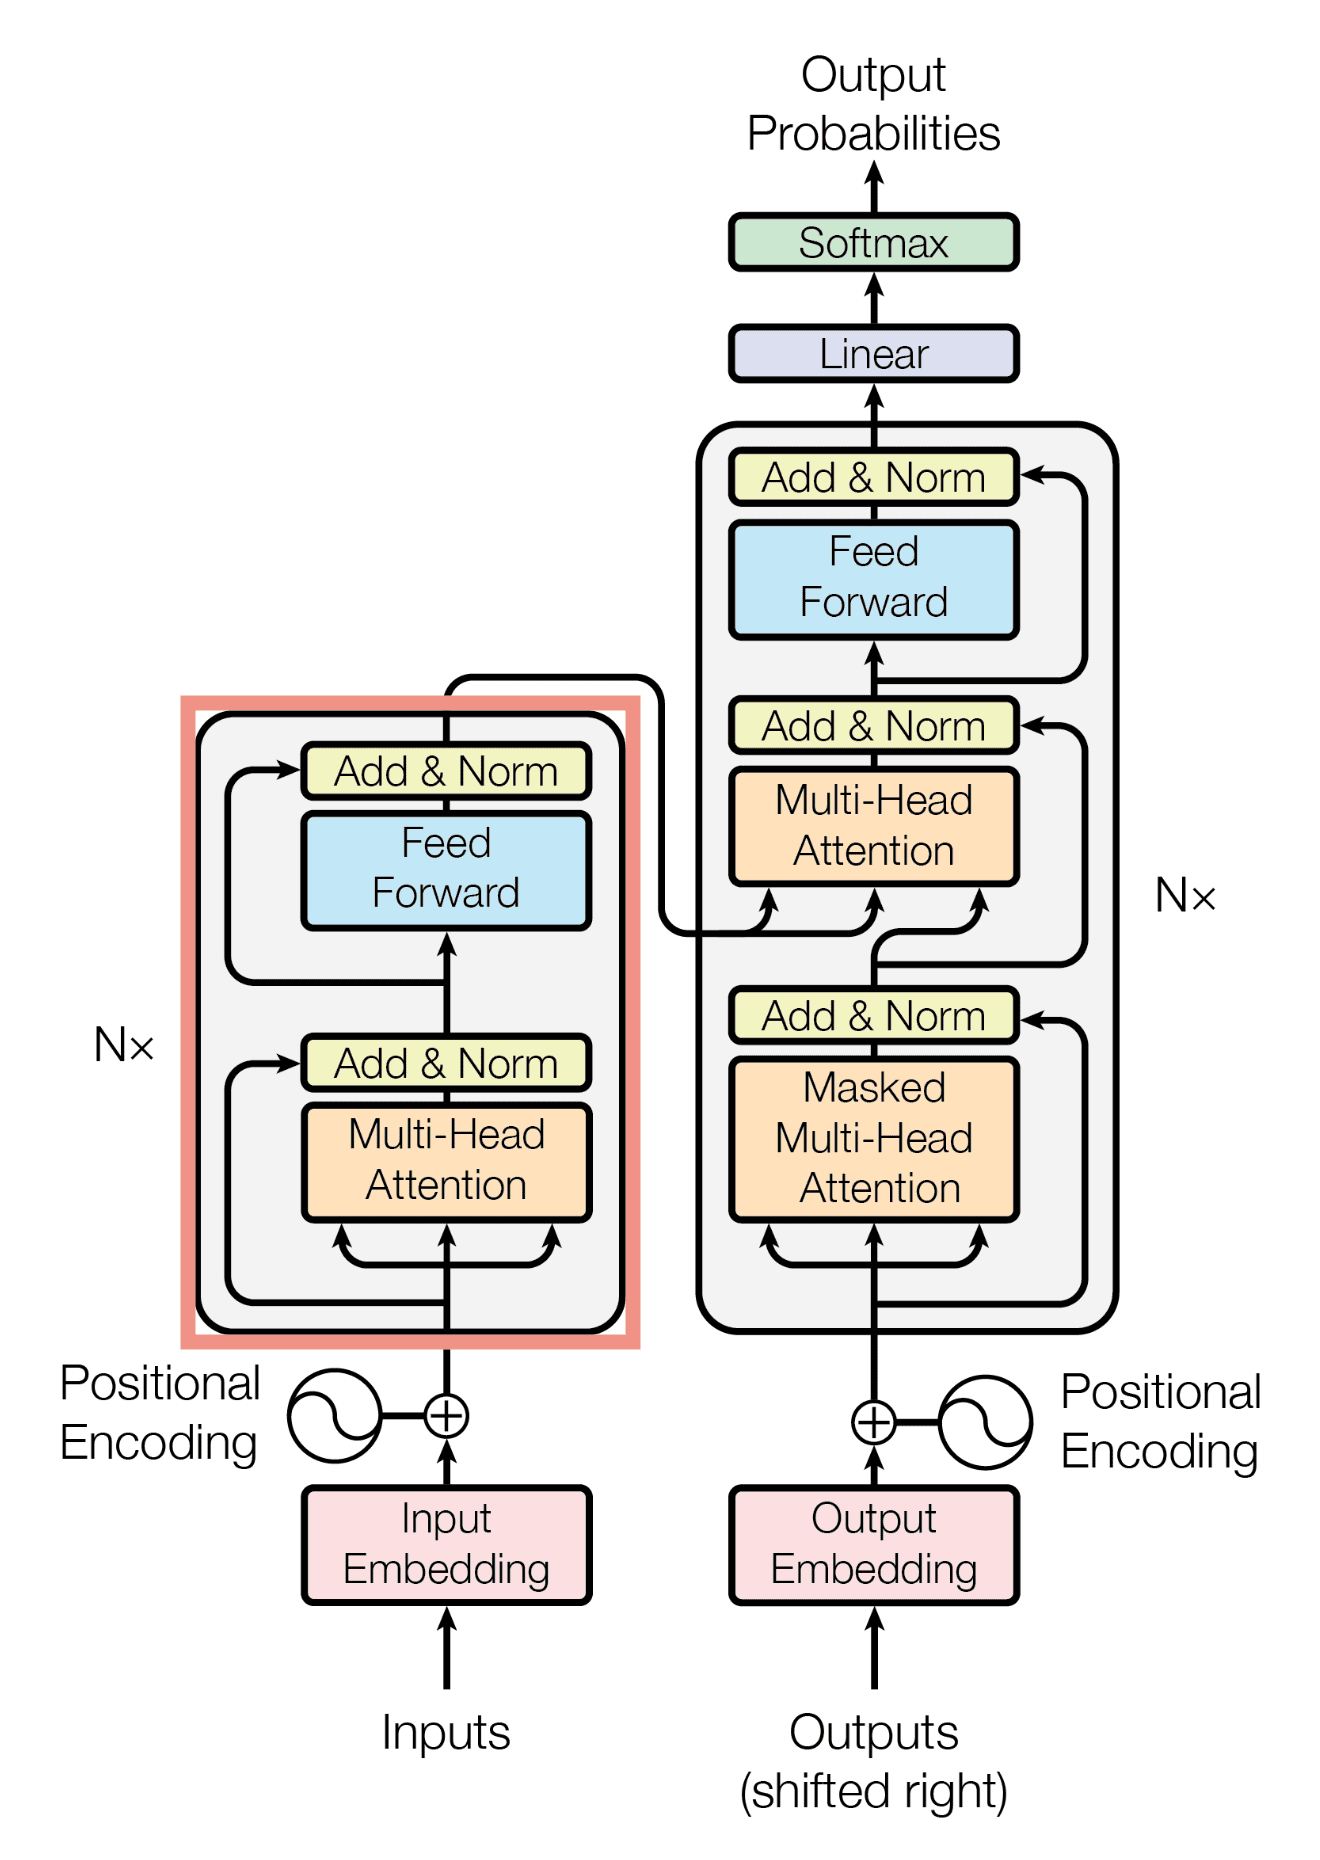
\includegraphics[width=0.35\textwidth]{./appunti_images/media/image29.png}
\caption{Struttura di un singolo blocco dell'encoder del Transformer: Multi-Head Self-Attention $\to$ Add \& Norm $\to$ FFN $\to$ Add \& Norm.}
\end{figure}

L'encoder è una pila di $N$ layer identici (nel paper originale $N = 6$). Ogni layer contiene:
\begin{enumerate}
\item \textbf{Multi-Head Self-Attention}
\item \textbf{Feed-Forward Network} (FFN)
\end{enumerate}
Ogni sotto-blocco è seguito da una \hyperref[app:residual]{\textbf{residual connection}} e \hyperref[app:layernorm]{\textbf{Layer Normalization}}:

\[
\text{output} = \text{LayerNorm}\!\bigl(\mathbf{x} + \text{Sublayer}(\mathbf{x})\bigr)
\]

\begin{notabox}[title={\textbf{LayerNorm, non BatchNorm}}]
Il Transformer usa \textbf{Layer Normalization}, che normalizza lungo la dimensione delle feature di ciascun singolo token, indipendentemente dal batch. Questo la rende adatta a sequenze di lunghezza variabile, a differenza della Batch Norm (vedi Appendice~\ref{app:layernorm}).
\end{notabox}

\begin{notabox}[title={\textbf{Pre-norm vs post-norm}}]
Il Transformer originale usa \textbf{post-norm}: $\text{LN}(\mathbf{x} + f(\mathbf{x}))$. Le architetture più recenti (GPT-2, Perceiver) usano \textbf{pre-norm}: $\mathbf{x} + f(\text{LN}(\mathbf{x}))$. La pre-norm è più stabile per reti molto profonde perché ogni sotto-blocco riceve input normalizzati, evitando che le attivazioni crescano in modo incontrollato.
\end{notabox}

\needspace{4\baselineskip}
\subsection{Scaled Dot-Product Attention}
\label{app:scaled-dot-product}

Il cuore del Transformer. L'input viene proiettato in tre spazi tramite matrici di peso apprese: \textbf{Query} ($\mathbf{Q}$), \textbf{Key} ($\mathbf{K}$), \textbf{Value} ($\mathbf{V}$).

\begin{figure}[htbp]
\centering
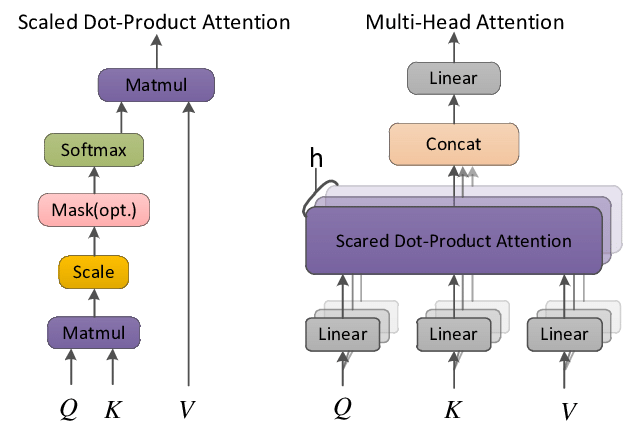
\includegraphics[width=0.40\textwidth]{./appunti_images/media/image30.png}
\caption{Schema della Scaled Dot-Product Attention (sinistra) e della Multi-Head Attention (destra).}
\end{figure}

\begin{formulabox}[title={\textbf{Scaled Dot-Product Attention}}]
\[
\text{Attention}(\mathbf{Q}, \mathbf{K}, \mathbf{V}) = \text{softmax}\!\left(\frac{\mathbf{Q}\mathbf{K}^\top}{\sqrt{d_k}}\right)\mathbf{V}
\]
\end{formulabox}

Interpretazione passo per passo:
\begin{enumerate}
\item \textbf{MatMul}: $\mathbf{Q}\mathbf{K}^\top \in \mathbb{R}^{M \times M}$ misura la \textbf{somiglianza} tra ogni coppia di token. L'elemento $(i,j)$ indica quanto il token $i$ è ``interessato'' al token $j$.
\item \textbf{Scale}: si divide per $\sqrt{d_k}$ per stabilizzare i gradienti.
\item \textbf{Mask} (opzionale): nel decoder, si pone $-\infty$ nelle posizioni future per impedire al modello di ``barare''.
\item \textbf{Softmax}: trasforma i punteggi in \textbf{pesi di attenzione} normalizzati (probabilità che sommano a 1 per ogni riga).
\item \textbf{MatMul}: si moltiplicano i pesi per $\mathbf{V}$ per ottenere la rappresentazione contestualizzata.
\end{enumerate}

\begin{formulabox}[title={\textbf{Perché dividere per $\sqrt{d_k}$?}}]
Se le componenti di $\mathbf{Q}$ e $\mathbf{K}$ hanno media 0 e varianza 1, il prodotto scalare $\mathbf{q} \cdot \mathbf{k} = \sum_{i=1}^{d_k} q_i k_i$ ha varianza $d_k$ (somma di $d_k$ prodotti indipendenti con varianza 1). Per valori grandi di $d_k$ (es. 64 o 128), i punteggi possono diventare molto grandi, spingendo la \hyperref[app:softmax]{softmax} in regioni di saturazione dove i gradienti sono quasi zero. Dividendo per $\sqrt{d_k}$ si riporta la varianza a $\sim 1$.
\end{formulabox}

\begin{figure}[htbp]
\centering

\includegraphics[width=0.50\textwidth]{./appunti_images/media/image32.png}
\caption{Dettaglio della Scaled Dot-Product Attention: il flusso da Q, K, V attraverso MatMul, Scale, Mask (opzionale) e Softmax.}
\end{figure}

\begin{notabox}[title={\textbf{Esempio numerico: attention su 3 token}}]
Supponiamo 3 token con $d_k = 2$:

$Q = \begin{pmatrix} 1 & 0 \\ 0 & 1 \\ 1 & 1 \end{pmatrix}$,
$K = \begin{pmatrix} 1 & 0 \\ 0 & 1 \\ 0.5 & 0.5 \end{pmatrix}$,
$V = \begin{pmatrix} 1 & 0 \\ 0 & 1 \\ 0.5 & 0.5 \end{pmatrix}$

\textbf{1. MatMul}: $QK^\top = \begin{pmatrix} 1 & 0 & 0.5 \\ 0 & 1 & 0.5 \\ 1 & 1 & 1 \end{pmatrix}$

\textbf{2. Scale}: $\frac{QK^\top}{\sqrt{2}} = \begin{pmatrix} 0.71 & 0 & 0.35 \\ 0 & 0.71 & 0.35 \\ 0.71 & 0.71 & 0.71 \end{pmatrix}$

\textbf{3. Softmax} (per riga): riga 1 $\to (0.43, 0.21, 0.30)$, riga 3 $\to (0.33, 0.33, 0.33)$

\textbf{Interpretazione}: il token 1 guarda soprattutto se stesso (0.43); il token 3 guarda tutti in modo uniforme (0.33) perché è ugualmente simile a tutti.
\end{notabox}

\needspace{4\baselineskip}
\subsection{Multi-Head Attention}

Invece di calcolare una sola attention con $d_k$ dimensioni, si calcolano $h$ ``teste'' in parallelo, ciascuna su uno spazio proiettato di dimensione ridotta $d_k/h$:

\begin{formulabox}[title={\textbf{Multi-Head Attention}}]
\[
\text{MultiHead}(\mathbf{Q}, \mathbf{K}, \mathbf{V}) = \text{Concat}(\text{head}_1, \ldots, \text{head}_h)\,\mathbf{W}^O
\]
\[
\text{head}_i = \text{Attention}\!\bigl(\mathbf{Q}\mathbf{W}_i^Q,\;\mathbf{K}\mathbf{W}_i^K,\;\mathbf{V}\mathbf{W}_i^V\bigr)
\]
con $\mathbf{W}_i^Q, \mathbf{W}_i^K \in \mathbb{R}^{d \times d_k}$, $\mathbf{W}_i^V \in \mathbb{R}^{d \times d_v}$, $\mathbf{W}^O \in \mathbb{R}^{hd_v \times d}$.

Nel Transformer originale: $d = 512$, $h = 8$, $d_k = d_v = d/h = 64$.
\end{formulabox}

Ogni testa impara a ``guardare'' un aspetto diverso (es.\ una si focalizza sulla sintassi, un'altra sulla semantica, un'altra sulle relazioni a lungo raggio). Le uscite vengono concatenate e proiettate da $\mathbf{W}^O$ per fondere le informazioni.

\begin{notabox}[title={\textbf{Perché multi-head e non single-head?}}]
Con una sola testa, il modello ha un'unica ``prospettiva'' per decidere a cosa prestare attenzione. Con $h$ teste, può catturare \emph{contemporaneamente} pattern diversi: relazioni sintattiche, semantiche, di prossimità, di riferimento, ecc. Il costo computazionale è lo stesso (ogni testa lavora su dimensione $d/h$), ma la capacità espressiva è molto maggiore.
\end{notabox}

\needspace{4\baselineskip}
\subsection{Feed-Forward Network (FFN)}

Dopo l'attention, ogni token passa indipendentemente attraverso un \textbf{MLP a due layer} (lo stesso per tutti i token):

\begin{formulabox}[title={\textbf{Feed-Forward Network}}]
\[
\text{FFN}(\mathbf{x}) = \text{ReLU}(\mathbf{x}\,\mathbf{W}_1 + \mathbf{b}_1)\,\mathbf{W}_2 + \mathbf{b}_2
\]
con $\mathbf{W}_1 \in \mathbb{R}^{d \times d_{ff}}$, $\mathbf{W}_2 \in \mathbb{R}^{d_{ff} \times d}$. Nel paper originale: $d = 512$, $d_{ff} = 2048$ (espansione $4\times$).
\end{formulabox}

\textbf{Perché serve l'FFN dopo l'attention?}
\begin{itemize}
\item L'attention è una \textbf{combinazione lineare pesata} dei Value: $Z = AV$. Da sola, non introduce non linearità.
\item L'FFN introduce \textbf{trasformazioni non lineari} (ReLU/\hyperref[app:activations]{GELU}), permettendo al modello di apprendere funzioni complesse.
\item L'espansione ($d \to 4d \to d$) aumenta la capacità senza cambiare la dimensione dell'output.
\end{itemize}

\needspace{4\baselineskip}
\subsection{Decoder}

\begin{figure}[htbp]
\centering
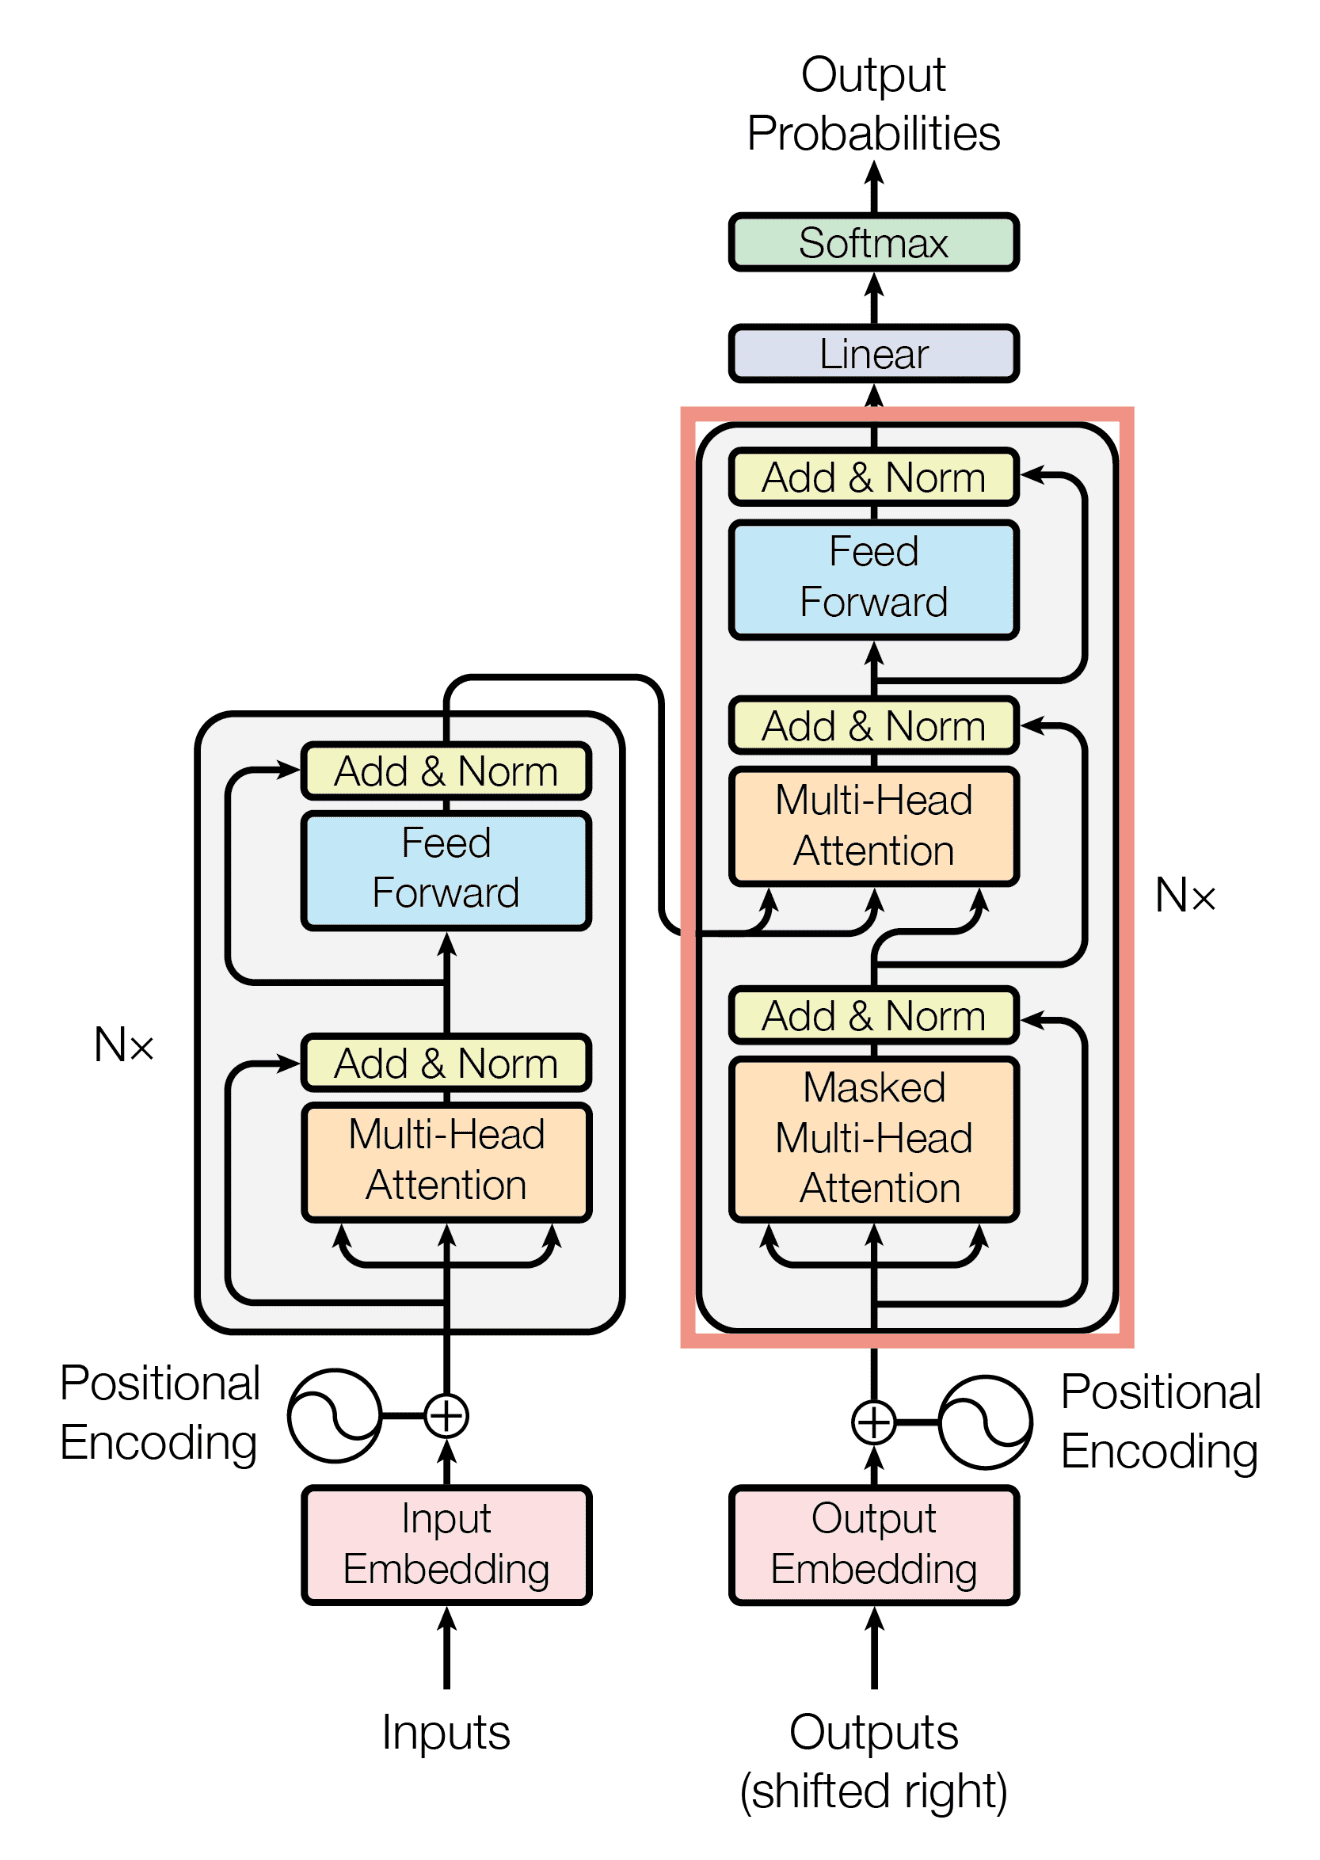
\includegraphics[width=0.35\textwidth]{./appunti_images/media/image31.png}
\caption{Struttura di un singolo blocco del decoder del Transformer con masked self-attention e cross-attention.}
\end{figure}

Il decoder ha una struttura simile all'encoder, ma con \textbf{tre} sotto-blocchi per layer:
\begin{enumerate}
\item \textbf{Masked Self-Attention}: impedisce al modello di ``guardare'' token futuri durante la generazione (masking causale: si pongono a $-\infty$ le posizioni $j > i$ nella matrice $QK^\top$, così la softmax le azzera).
\item \textbf{Cross-Attention}: le \textbf{Query vengono dal decoder}, ma \textbf{Key e Value dall'output dell'encoder}. Questo permette al decoder di ``leggere'' la rappresentazione dell'input per generare l'output.
\item \textbf{FFN}: identico a quello dell'encoder.
\end{enumerate}

L'output finale passa attraverso una proiezione lineare $\mathbf{W} \in \mathbb{R}^{d \times |\text{vocab}|}$ + softmax per generare la distribuzione di probabilità sul vocabolario ad ogni passo temporale.

\begin{notabox}[title={\textbf{Esempio: traduzione ``Il gatto dorme'' $\to$ ``The cat sleeps''}}]
\textbf{Encoder}: prende [``Il'', ``gatto'', ``dorme''] $\to$ embedding + PE $\to$ 6 blocchi encoder $\to$ rappresentazione contestualizzata $\mathbf{H} \in \mathbb{R}^{3 \times 512}$.

\textbf{Decoder} (autoregressivo, genera un token alla volta):
\begin{itemize}
\item Passo 1: input [BOS] $\to$ masked self-attn $\to$ cross-attn (legge $\mathbf{H}$) $\to$ FFN $\to$ softmax $\to$ ``The''
\item Passo 2: input [BOS, The] $\to$ masked self-attn (The non vede il futuro) $\to$ cross-attn $\to$ softmax $\to$ ``cat''
\item Passo 3: input [BOS, The, cat] $\to$ $\ldots$ $\to$ ``sleeps''
\item Passo 4: $\to$ [EOS] (fine generazione)
\end{itemize}
Durante il \textbf{training} si usa \emph{teacher forcing}: si fornisce l'output corretto come input del decoder, non la predizione precedente.
\end{notabox}

\begin{figure}[htbp]
\centering

\includegraphics[width=0.40\textwidth]{./appunti_images/papers/fig_attention_heatmap.png}
\caption{Matrice di attenzione nella traduzione inglese$\to$francese (Bahdanau et al., 2014). Le celle chiare indicano alta attenzione: il modello impara automaticamente l'allineamento tra parole. (Fonte: Lilian Weng)}
\label{fig:attention_heatmap}
\end{figure}

\needspace{4\baselineskip}
\subsection{Positional Encoding}

\begin{formulabox}[title={\textbf{Positional Encoding sinusoidale}}]
L'attenzione è \textbf{invariante per permutazione}: senza informazione posizionale, il Transformer non distingue ``il gatto mangia il topo'' da ``il topo mangia il gatto''. Il positional encoding risolve questo problema:

\[
\text{PE}(\text{pos}, 2i) = \sin\!\left(\frac{\text{pos}}{10000^{2i/d}}\right) \qquad
\text{PE}(\text{pos}, 2i+1) = \cos\!\left(\frac{\text{pos}}{10000^{2i/d}}\right)
\]
Le frequenze decrescono geometricamente: le prime dimensioni oscillano rapidamente (distinguono posizioni vicine), le ultime lentamente (catturano la struttura globale). \textbf{Proprietà chiave:} $\text{PE}(\text{pos}+k)$ può essere espresso come trasformazione lineare di $\text{PE}(\text{pos})$, permettendo al modello di apprendere relazioni posizionali relative.
\end{formulabox}

\begin{notabox}[title={\textbf{Differenza con il Perceiver}}]
Il Transformer \textbf{somma} il positional encoding all'embedding ($z = \text{embed} + \text{PE}$), mescolando contenuto e posizione. Il Perceiver \textbf{concatena} le Fourier features all'input ($z = [\text{contenuto} \| \text{PE}]$), preservando le informazioni separatamente. Inoltre, il Perceiver usa Fourier features multiscala con frequenze esponenziali, non le sinusoidi fisse del Transformer.
\end{notabox}

\needspace{4\baselineskip}
\subsection{Riassunto e confronto con il Perceiver}

{\small
\begin{longtable}{@{}p{3cm}p{5cm}p{5cm}@{}}
\toprule
\textbf{Aspetto} & \textbf{Transformer} & \textbf{Perceiver} \\
\midrule\endhead
\bottomrule\endlastfoot
Input & Sequenza di token (testo, tipicamente $M < 1024$) & Qualsiasi modalità (pixel, byte, campioni audio, $M$ fino a 50K+) \\
Tokenizzazione & Necessaria (BPE, SentencePiece) & Non necessaria (lavora su byte/pixel grezzi) \\
Tipo di attention & Self-attention ($Q,K,V$ tutti da $X$) & Cross-attention ($Q$ da latenti, $K,V$ da input) \\
Complessità & $O(M^2 d)$ per layer & $O(MNd)$ cross-att + $O(N^2 d)$ latent \\
Positional Encoding & Somma (sinusoidale o appreso) & Concatenazione (Fourier features) \\
Profondità & $N$ layer (tipicamente 6--12) & $T$ iterazioni (tipicamente 8) con weight sharing \\
Output & Sequenza (encoder-decoder) & Classificazione (pooling) o output queries (Perceiver IO) \\
Attivazione FFN & ReLU & GELU \\
Normalizzazione & Post-norm (originale) & Pre-norm \\
\end{longtable}
}

\begin{notabox}[title={\textbf{Collegamento al Perceiver}}]
Il Perceiver \textbf{sostituisce la self-attention} (costo $O(M^2)$) \textbf{con la cross-attention} (costo $O(MN)$, dove $N \ll M$). Per un'immagine $224 \times 224$: $M = 50{,}176$ pixel, ma $N = 512$ latenti, riducendo la complessità di $\sim\!100\times$. Tuttavia, il Perceiver \emph{eredita} dal Transformer tutti gli altri componenti: multi-head attention, FFN, residual connections, LayerNorm.
\end{notabox}

Il Transformer funziona su sequenze 1D (testo). Per applicarlo alle immagini, il Vision Transformer (ViT) introduce un modo elegante di ``tokenizzare'' un'immagine.

% ---------------------------------------------------------------------------

\section{Vision Transformer (ViT)}
\label{app:vit}

Il \textbf{Vision Transformer} (Dosovitskiy et al., 2021, ICLR) applica il Transformer alle immagini, trattandole come sequenze di \textbf{patch}. Invece di usare convoluzioni, divide l'immagine in blocchi regolari, li proietta in embedding e li elabora con un encoder Transformer standard.

\begin{notabox}[title={\textbf{Motivazione: perché applicare il Transformer alle immagini?}}]
Le CNN sono ottime grazie ai loro inductive bias (località, invarianza traslazionale), ma non catturano facilmente le \textbf{dipendenze globali}: un pixel in alto a sinistra non ``vede'' direttamente un pixel in basso a destra senza molti strati. Il ViT usa l'attenzione per creare dipendenze globali fin dal primo strato: ogni patch può interagire con qualsiasi altra patch. Il prezzo è la necessità di dataset molto grandi o pretraining + fine-tuning.
\end{notabox}

\begin{figure}[htbp]
\centering
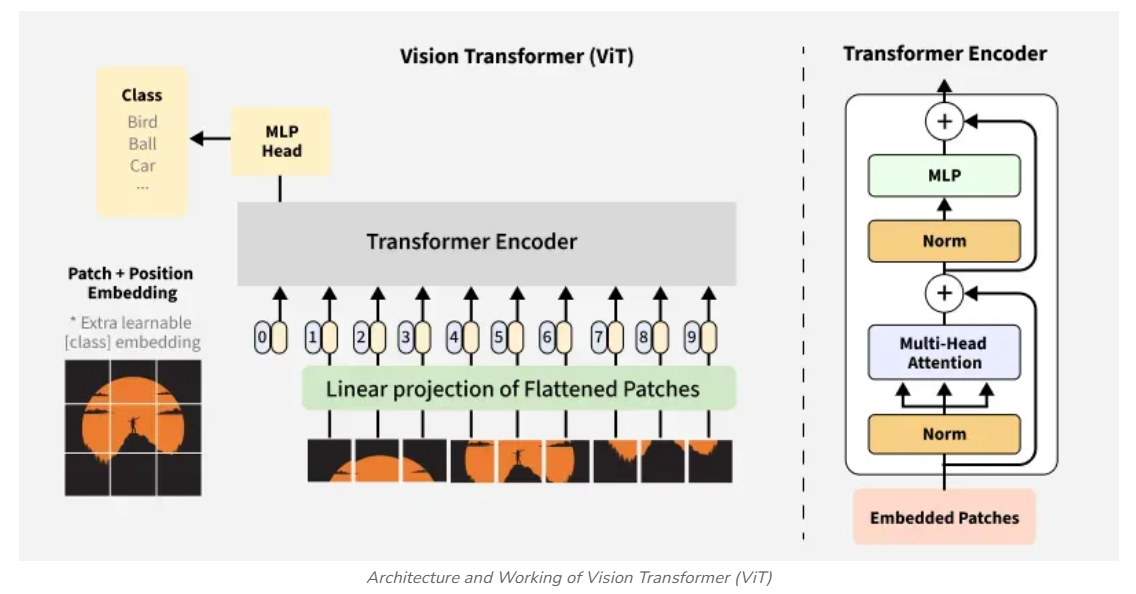
\includegraphics[width=0.65\textwidth]{./appunti_images/media/image33.png}
\caption{Pipeline del Vision Transformer (ViT): patch splitting, embedding e encoder Transformer.}
\end{figure}

\needspace{4\baselineskip}
\subsection{Pipeline completa}

\needspace{3\baselineskip}
\subsubsection{1. Patch Splitting}
L'immagine $I \in \mathbb{R}^{224 \times 224 \times 3}$ viene divisa in patch $16 \times 16$ non sovrapposte:

\[
N = \frac{224}{16} \times \frac{224}{16} = 14 \times 14 = 196 \text{ patch}
\]

\needspace{3\baselineskip}
\subsubsection{2. Flattening}
Ogni patch ($16 \times 16 \times 3 = 768$ valori) viene appiattito in un vettore 1D:

\[
\mathbf{p}_i \in \mathbb{R}^{768}, \quad i = 1, \ldots, 196
\]

\needspace{3\baselineskip}
\subsubsection{3. Linear Projection (Patch Embedding)}
Una proiezione lineare apprendibile trasforma ogni patch:

\[
\mathbf{x}_i = \mathbf{p}_i\,\mathbf{W}_E + \mathbf{b}_E, \quad \mathbf{W}_E \in \mathbb{R}^{768 \times D}
\]
Con $D = 768$ (ViT-Base), ogni patch diventa un embedding di 768 dimensioni.

\needspace{3\baselineskip}
\subsubsection{4. CLS Token}
Si prepone un \textbf{token speciale} $\mathbf{z}_{\text{CLS}} \in \mathbb{R}^{D}$ alla sequenza. Il CLS raccoglie informazione da tutti i patch tramite self-attention e viene usato per la classificazione finale.

\[
\mathbf{X}' = [\mathbf{z}_{\text{CLS}},\; \mathbf{x}_1,\; \mathbf{x}_2,\; \ldots,\; \mathbf{x}_{196}] \in \mathbb{R}^{197 \times 768}
\]

\needspace{3\baselineskip}
\subsubsection{5. Positional Encoding}
Si sommano \textbf{positional embedding apprendibili} per codificare la posizione spaziale:

\[
\mathbf{Z}^0 = \mathbf{X}' + \mathbf{P}, \quad \mathbf{P} \in \mathbb{R}^{197 \times 768}
\]

\begin{formulabox}[title={\textbf{Formula compatta del ViT}}]
\[
\mathbf{z}_0 = [\mathbf{x}_{\text{class}};\; \mathbf{x}_1\mathbf{E};\; \mathbf{x}_2\mathbf{E};\; \ldots;\; \mathbf{x}_P\mathbf{E}] + \mathbf{E}_{\text{pos}} \in \mathbb{R}^{(P+1) \times D}
\]
dove $P = 196$ è il numero di patch, $\mathbf{x}_i$ è la patch $i$ appiattita, $\mathbf{E} \in \mathbb{R}^{(16^2 \cdot 3) \times D}$ è la matrice di proiezione, e $\mathbf{E}_{\text{pos}} \in \mathbb{R}^{(P+1) \times D}$ sono i positional embedding appresi.
\end{formulabox}

\needspace{3\baselineskip}
\subsubsection{6. Transformer Encoder ($L = 12$ layer)}

Ogni encoder layer:
\begin{enumerate}
\item LayerNorm $\to$ Multi-Head Self-Attention $\to$ Residual connection
\item LayerNorm $\to$ FFN (GELU) $\to$ Residual connection
\end{enumerate}

\paragraph{a) Multi-Head Self-Attention}

Per $\mathbf{Z}^{l-1} \in \mathbb{R}^{197 \times 768}$, con $h = 12$ teste ($d_k = 64$ ciascuna):

\[
\mathbf{Q} = \mathbf{Z}^{l-1}\mathbf{W}^Q, \quad
\mathbf{K} = \mathbf{Z}^{l-1}\mathbf{W}^K, \quad
\mathbf{V} = \mathbf{Z}^{l-1}\mathbf{W}^V
\]
\[
\text{head}_i = \text{softmax}\!\left(\frac{\mathbf{Q}_i\mathbf{K}_i^\top}{\sqrt{64}}\right)\mathbf{V}_i
\qquad
\text{MHA} = \text{Concat}(\text{head}_1, \ldots, \text{head}_{12})\,\mathbf{W}^O
\]

\paragraph{b) Feed Forward Network}

\[
\text{FFN}(\mathbf{z}) = \text{GELU}(\mathbf{z}\,\mathbf{W}_1 + \mathbf{b}_1)\,\mathbf{W}_2 + \mathbf{b}_2
\]
con $\mathbf{W}_1 \in \mathbb{R}^{768 \times 3072}$ (espansione) e $\mathbf{W}_2 \in \mathbb{R}^{3072 \times 768}$ (compressione).

\needspace{3\baselineskip}
\subsubsection{7. Classificazione (MLP Head)}

Dopo $L = 12$ layer: $\mathbf{Z}^{12} \in \mathbb{R}^{197 \times 768}$.

Si estrae il CLS token: $\mathbf{z}_{\text{CLS}}^{(12)} = \mathbf{Z}^{12}[0] \in \mathbb{R}^{768}$

\begin{formulabox}[title={\textbf{Classificazione finale}}]
\[
\hat{\mathbf{y}} = \text{softmax}\!\bigl(\mathbf{W}_{\text{cls}}\,\mathbf{z}_{\text{CLS}}^{(12)} + \mathbf{b}\bigr),
\quad \mathbf{W}_{\text{cls}} \in \mathbb{R}^{K \times 768}
\]
\end{formulabox}

\needspace{4\baselineskip}
\subsection{ViT vs CNN: differenze fondamentali}

\textbf{1. Local vs.\ Global Attention}
\begin{itemize}
\item \textbf{CNN:} filtri locali (es.\ $3 \times 3$), il contesto globale si costruisce solo gradualmente nei layer profondi.
\item \textbf{ViT:} self-attention globale fin dal primo layer --- ogni patch ``parla'' con tutti gli altri.
\end{itemize}

\textbf{2. Inductive Biases}
\begin{itemize}
\item \textbf{CNN:} bias induttivi forti (localit\`a, invarianza alla traslazione) $\to$ efficienti con pochi dati.
\item \textbf{ViT:} pochi bias induttivi $\to$ pi\`u flessibile ma necessita di dataset molto grandi (ImageNet-21k, JFT-300M) o pretraining + fine-tuning.
\end{itemize}

\textbf{3. Training Data Requirements}
\begin{itemize}
\item \textbf{CNN:} performano bene anche con dataset medio-piccoli (CIFAR-10, MNIST).
\item \textbf{ViT:} richiedono pretraining su dataset enormi; dominano quando i dati abbondano.
\end{itemize}

\begin{notabox}[title={\textbf{Collegamento al Perceiver}}]
Il ViT riduce la dimensione dell'input da $M = 50{,}176$ pixel a $M = 196$ patch tramite la tokenizzazione, ma questa resta \textbf{domain-specific} (funziona solo per immagini). Il Perceiver elimina completamente la tokenizzazione domain-specific: accetta \emph{qualsiasi} input (pixel grezzi, audio, point cloud) e usa la cross-attention per proiettarlo in un latent array di dimensione fissa $N \ll M$.
\end{notabox}

\section{Complementi: Self-Attention vs Cross-Attention}
\label{app:self-vs-cross}

\begin{figure}[htbp]
\centering
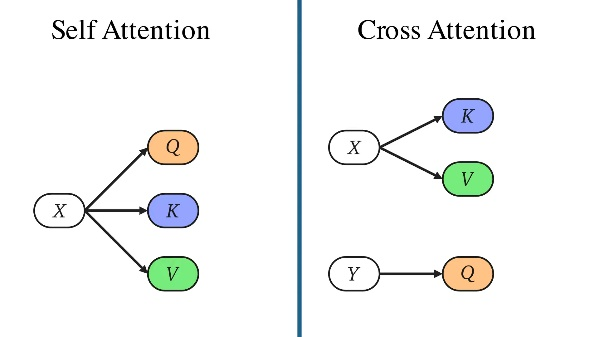
\includegraphics[width=0.65\textwidth]{./appunti_images/media/image89.jpeg}
\caption{Confronto tra self-attention e cross-attention: nella self-attention Q, K, V provengono dallo stesso input; nella cross-attention provengono da sorgenti diverse.}
\end{figure}

\textbf{Differenza
tra Self-attention e Cross-attention}

La \textbf{self-attention} è un meccanismo in cui \textbf{Query (Q),
Key (K) e Value (V) provengono tutti dallo stesso insieme di input}.

\begin{itemize}
\item
  Serve a far sì che ogni elemento della sequenza (o ogni latente)
  \textbf{interagisca con gli altri} per arricchire la propria
  rappresentazione.
\item
  Input $I$: sequenza di token (parole o patch immagine).

\[
I \in \mathbb{R}^{M \times D}
\]
Si calcolano direttamente:

\[
Q = I W_Q, \quad K = I W_K, \quad V = I W_V
\]
Attenzione:

\[
A = \text{Softmax}\left(\frac{Q K^T}{\sqrt{d_k}}\right) \in \mathbb{R}^{M \times M}
\]
Output:

\[
Z = A \cdot V \in \mathbb{R}^{M \times D}
\]È
  quindi un'operazione \textbf{intra-spazio}: lo stesso array si
  auto-analizza e si rielabora.
\end{itemize}

(nel caso dei trasformer con M molto grande il calcolo diventa
proibitivo)

La \textbf{cross-attention} è un meccanismo in cui \textbf{Query (Q)
proviene da un insieme (es. i latenti)} e \textbf{Key (K), Value (V)
provengono da un altro insieme (es. l'immagine/token di input)}.

\begin{itemize}
\item
  Serve a permettere a un insieme (latenti) di \textbf{interrogare un
  altro insieme} (input esterno) e di incorporarne l'informazione.
\item
  È quindi un'operazione \textbf{inter-spazio}: un array aggiorna la
  propria rappresentazione ``guardando'' un altro array.
\end{itemize}

Formula:

\[
A = \text{Softmax}\left(\frac{Q K^T}{\sqrt{d_k}}\right), \quad Z = A \cdot V
\]
con $Q$ dai latenti $L$, e $K, V$ dall'immagine $I$.

\textbf{Differenza tra Single-Head Cross-Attention e Multi-Head
Cross-Attention nel Perceiver}

\begin{notabox}
Negli esempi seguenti usiamo $D = 1024$ e $d_k = D/h = 1024/8 = 128$, coerentemente con la configurazione ImageNet del paper. Per single-head, la dimensione dello spazio di proiezione coincide con $D$.
\end{notabox}

\textbf{1. Single-Head Cross-Attention}
\begin{enumerate}
\item Proiezioni lineari:
\begin{align*}
Q &= L W^Q \quad (512 \times 1024 \to 512 \times 1024) \\
K &= X W^K, \quad V = X W^V \quad (50176 \times 1024 \to 50176 \times 1024)
\end{align*}
\item Attenzione:

\[
A = \text{softmax}\!\left(\frac{QK^\top}{\sqrt{1024}}\right) \quad (512 \times 50176)
\]
\item Output:

\[
\text{Out} = A V \quad (512 \times 1024)
\]
\end{enumerate}
Ogni latente interroga l'intera immagine con un'\textbf{unica} mappa di attenzione.

\textbf{2. Multi-Head Cross-Attention} ($h = 8$)

\begin{enumerate}
\item Divisione embedding:

\[
d_k = \frac{D}{h} = \frac{1024}{8} = 128
\]
\item Proiezioni per ogni testa $i$:
\begin{align*}
Q_i &= L W_i^Q \quad (512 \times 1024 \to 512 \times 128) \\
K_i &= X W_i^K, \quad V_i = X W_i^V \quad (50176 \times 1024 \to 50176 \times 128)
\end{align*}
\item Attenzione per ogni testa:

\[
A_i = \text{softmax}\!\left(\frac{Q_i K_i^\top}{\sqrt{128}}\right) \quad (512 \times 50176)
\]
\[
\text{head}_i = A_i V_i \quad (512 \times 128)
\]
\item Concatenazione e proiezione finale:

\[
\text{Out} = \text{Concat}(\text{head}_1, \ldots, \text{head}_8) W^O \quad (512 \times 1024)
\]
\end{enumerate}
Ogni latente interroga l'immagine con 8 \textbf{mappe di attenzione diverse} --- viste parallele su pattern differenti (colore, bordi, texture, struttura globale).

\textbf{Definizione di $W^O$}

Dopo aver calcolato tutte le teste:

\[
\text{head}_i = \text{Attention}(Q_i, K_i, V_i) \quad \in \mathbb{R}^{N \times d_k}
\]
Concateno i risultati:

\[
H = \text{Concat}(\text{head}_1, \ldots, \text{head}_h) \quad \in \mathbb{R}^{N \times (h \cdot d_k)}
\]
Poiché $h \cdot d_k = D$, abbiamo $H \in \mathbb{R}^{N \times D}$.

A questo punto si applica una proiezione lineare con matrice $W^O$:

\[
\text{Out} = H W^O, \quad W^O \in \mathbb{R}^{D \times D}
\]

\textbf{A cosa serve $W^O$}
\begin{enumerate}
\item \textbf{Ricombinare le teste}: Ogni testa produce una rappresentazione parziale (es. bordi, colore, posizione). La concatenazione è solo un ``accostamento''. $W^O$ permette di \textbf{mescolare e fondere} queste informazioni in un'unica rappresentazione coerente nello spazio di dimensione $D$.
\item \textbf{Mantenere la dimensione costante}: Input e output della Multi-Head Attention devono restare nella stessa dimensione $D$ (nel Perceiver: 1024 per ImageNet). Senza $W^O$, l'output sarebbe solo una concatenazione, priva di trasformazione finale.
\item \textbf{Parametri appresi}: $W^O$ è una matrice di peso appresa tramite backpropagation. Inizializzata (es. Xavier uniform), si aggiorna durante il training. Serve a \textbf{decidere come pesare} le informazioni provenienti dalle varie teste.
\end{enumerate}

\textbf{3. Confronto diretto}

\begin{center}
\begin{tabular}{l l l}
\hline
\textbf{Aspetto} & \textbf{Single-Head} & \textbf{Multi-Head (h=8)} \\
\hline
Dimensione Q & $512 \times 1024$ & $8 \times 512 \times 128$ \\
Dimensione K,V & $50176 \times 1024$ & $8 \times 50176 \times 128$ \\
Pesi di attenzione & 1 matrice $512 \times 50176$ & 8 matrici $512 \times 50176$ \\
Output testa & $512 \times 1024$ & $8 \times 512 \times 128 \to$ concat $\to 512 \times 1024$ \\
Capacità & Una sola prospettiva & Più prospettive parallele (pattern diversi) \\
\hline
\end{tabular}
\end{center}

\textbf{Differenza concettuale}
\begin{itemize}
\item Le matrici $W^Q, W^K, W^V$ servono a \textbf{proiettare} l'input in spazi diversi per calcolare l'attenzione.
\item La matrice $W^O$ serve a \textbf{ricombinare} i risultati delle teste e riportarli nello spazio embedding originale.
\end{itemize}

\textbf{Nel Perceiver (ImageNet)}:

\begin{itemize}
\item $D = 1024$, $h = 8$ teste
\item Ogni testa: $d_k = 128$
\item Dopo la concat: $H \in \mathbb{R}^{512 \times 1024}$
\item Moltiplicazione con $W^O \in \mathbb{R}^{1024 \times 1024}$ $\to$ output finale $N \times 1024$
\end{itemize}

\textbf{Multi-Head Attention (MHA) in generale}

In un layer Transformer (o Perceiver), non usiamo una sola attenzione ma
più teste parallele.

Ogni testa ha i suoi pesi \(W_{Q},W_{K},W_{V}\) e calcola:

\[Z_{h} = Softmax\left( \frac{Q_{h}K_{h}^{T}}{\sqrt{D_{h}}} \right)V_{h}\]

\(conD_{h} = D/H\) (dimensione ridotta se ci sono \(H\) teste).

\begin{itemize}
\item
  Poi i risultati di tutte le teste vengono concatenati e proiettati con
  un altro peso \(W_{O}\) :
\end{itemize}

\[Z = Concat\left( Z_{1},\ldots,Z_{H} \right)W_{O}\]

Quindi la MHA è una struttura architetturale che moltiplica la capacità
del modello di guardare in più "spazi" o "prospettive".

\needspace{3\baselineskip}
\subsubsection{\texorpdfstring{\textbf{Cosa cambia sostanzialmente con
tipi di input diversi nel
Perceiver?}}{Cosa cambia sostanzialmente con tipi di input diversi nel Perceiver?}}\label{cosa-cambia-sostanzialmente-con-tipi-di-input-diversi-nel-perceiver}

Sostanzialmente, ciò che cambia è solo il \textbf{modo in cui
l'input grezzo viene trasformato in un array di byte
bidimensionale (la matrice M x C)} prima di essere processato dal
modello. Il cuore dell'architettura Perceiver, ovvero il
meccanismo di cross-attenzione che astrae l'input in un
array latente di dimensione fissa e i successivi blocchi Transformer,
\textbf{rimane quasi identico}.

Questa è la vera forza del Perceiver: disaccoppiare
l'elaborazione principale dalla specificità
dell'input. Il modello non ha bisogno di
un'architettura completamente diversa per ogni tipo di
dato, ma solo di una strategia di "appiattimento" e codifica posizionale
iniziale.

Vediamo le differenze specifiche per ogni caso.

\needspace{3\baselineskip}
\subsubsection{\texorpdfstring{\textbf{Come cambiano le matrici e gli
step
successivi}}{Come cambiano le matrici e gli step successivi}}\label{come-cambiano-le-matrici-e-gli-step-successivi}

\paragraph{\texorpdfstring{\textbf{1.
Immagine}}{1. Immagine}}\label{immagine}

\begin{itemize}
\item
  \textbf{Matrice di Input (M x C)}: Per un'immagine, la
  trasformazione è molto diretta. L'immagine, con le sue
  dimensioni spaziali (altezza H, larghezza W) e i suoi canali di colore
  (es. 3 per RGB), viene "appiattita".

\begin{itemize}
  \item
    \textbf{M (numero di elementi)}: Diventa H * W. Ogni pixel è un
    elemento dell'array di input.
  \item
    \textbf{C (dimensione di ogni elemento)}: Corrisponde ai canali del
    pixel (es. 3 per i valori R, G, B) a cui si aggiunge una codifica
    posizionale (positional encoding) per preservare
    l'informazione spaziale. Questa codifica è
    fondamentale, altrimenti il modello vedrebbe solo un "sacco di
    pixel" senza sapere dove si trovavano.
  \item
    \textbf{Esempio}: Un'immagine 224x224 RGB diventa
    una matrice M x C di (224*224) x (3 + D\_pos), dove M = 50.176 e
    D\_pos è la dimensione della codifica posizionale.
  \end{itemize}
\item
  \textbf{Matrice Latente (N x D)}: Questa matrice è
  \textbf{indipendente dall'input}. La sua dimensione è
  un iperparametro del modello che tu definisci a priori.

\begin{itemize}
  \item
    \textbf{N (numero di vettori latenti)}: È fisso (es. 512). Questo
    determina la "larghezza di banda" computazionale del modello. È
    molto più piccolo di M.
  \item
    \textbf{D (dimensione di ogni vettore latente)}: È
    anch'esso fisso (es. 1024).
  \end{itemize}
\item
  \textbf{Step Successivi}:

\begin{itemize}
  \item
    \textbf{Cross-Attention}: L'array latente (N x D),
    che è inizializzato casualmente, "guarda" l'enorme
    array di input (M x C) e, tramite la cross-attenzione, estrae le
    informazioni più salienti, "comprimendole" in sé stesso.
    L'array latente funge da \emph{query}, mentre
    l'array di input funge da \emph{key} e \emph{value}.
  \item
    \textbf{Self-Attention (Transformer Blocks)}:
    L'array latente N x D, ora "carico" di informazioni
    dall'immagine, viene processato da una serie di
    blocchi Transformer standard (self-attention). Qui, i vettori
    latenti interagiscono tra loro per affinare e integrare le
    informazioni estratte.
  \item
    \textbf{Classificazione Finale}: L'output del blocco
    Transformer (ancora di dimensione N x D) viene mediato (average
    pooling) lungo la dimensione N per ottenere un singolo vettore di
    dimensione D. Questo vettore viene poi dato in input a una testa di
    classificazione (un semplice layer lineare) per produrre i
    \textbf{logits} finali.
  \end{itemize}
\end{itemize}

\paragraph{\texorpdfstring{\textbf{2. Video}}{2. Video}}\label{video}

\begin{itemize}
\item
  \textbf{Matrice di Input (M x C)}: Un video è una sequenza di frame
  (immagini) nel tempo. L'appiattimento include anche la
  dimensione temporale.

\begin{itemize}
  \item
    \textbf{M (numero di elementi)}: Diventa T * H * W, dove T è il
    numero di frame.
  \item
    \textbf{C (dimensione di ogni elemento)}: Come per
    l'immagine, include i canali del pixel (es. 3) più
    una codifica posizionale. Crucialmente, questa codifica deve
    rappresentare non solo la posizione (x, y) nel frame, ma anche la
    posizione temporale t.
  \item
    \textbf{Esempio}: Un video di 16 frame 224x224 diventa una matrice M
    x C di (16*224*224) x (3 + D\_pos\_3D), con M = 802.816.
  \end{itemize}
\item
  \textbf{Matrice Latente (N x D)}: \textbf{Non cambia}. È sempre la
  stessa matrice di dimensione fissa N x D definita come iperparametro.
\item
  \textbf{Step Successivi}: \textbf{Identici al caso
  dell'immagine}. Il meccanismo di cross-attenzione non
  si "preoccupa" del fatto che l'input provenga da
  un'immagine o da un video. Semplicemente, interroga un
  array di byte molto più grande, che grazie alla codifica posizionale
  contiene implicitamente l'informazione
  spazio-temporale.
\end{itemize}

\paragraph{\texorpdfstring{\textbf{3. Nuvola di Punti (Point
Cloud)}}{3. Nuvola di Punti (Point Cloud)}}\label{nuvola-di-punti-point-cloud}

\begin{itemize}
\item
  \textbf{Matrice di Input (M x C)}: Una nuvola di punti è un insieme di
  punti in uno spazio 3D.

\begin{itemize}
  \item
    \textbf{M (numero di elementi)}: È semplicemente il numero di punti
    nella nuvola.
  \item
    \textbf{C (dimensione di ogni elemento)}: Per ogni punto, le feature
    sono le sue coordinate (x, y, z). A queste si possono aggiungere
    altre informazioni come il colore (R, G, B) o la normale. A
    differenza delle immagini, qui non è necessaria una codifica
    posizionale esplicita, perché le coordinate (x, y, z) sono già
    l'informazione posizionale stessa.
  \item
    \textbf{Esempio}: Una nuvola di 4096 punti con coordinate e colori
    diventa una matrice M x C di 4096 x 6.
  \end{itemize}
\item
  \textbf{Matrice Latente (N x D)}: Ancora una volta, \textbf{non
  cambia}. La sua dimensione è fissa.
\item
  \textbf{Step Successivi}: Esattamente gli stessi. La matrice latente N
  x D usa la cross-attenzione per interrogare la matrice di punti M x C
  e distillare l'informazione rilevante. Il resto del
  processo fino ai logits è invariato.
\end{itemize}

\needspace{3\baselineskip}
\subsubsection{\texorpdfstring{\textbf{Tabella
Riassuntiva}}{Tabella Riassuntiva}}\label{tabella-riassuntiva}

{\def\LTcaptype{none} % do not increment counter
\begin{longtable}{@{}
  >{\raggedright\arraybackslash}p{(\linewidth - 6\tabcolsep) * \real{0.1172}}
  >{\raggedright\arraybackslash}p{(\linewidth - 6\tabcolsep) * \real{0.3543}}
  >{\raggedright\arraybackslash}p{(\linewidth - 6\tabcolsep) * \real{0.2152}}
  >{\raggedright\arraybackslash}p{(\linewidth - 6\tabcolsep) * \real{0.3133}}@{}}
\toprule\noalign{}
\begin{minipage}[b]{\linewidth}\raggedright
Tipo di Input
\end{minipage} & \begin{minipage}[b]{\linewidth}\raggedright
Matrice di Input (M x C)
\end{minipage} & \begin{minipage}[b]{\linewidth}\raggedright
Matrice Latente (N x D)
\end{minipage} & \begin{minipage}[b]{\linewidth}\raggedright
Note
\end{minipage} \\
\midrule\noalign{}
\endhead
\bottomrule\noalign{}
\endlastfoot
\textbf{Immagine} & M = H * W, C = Canali + Pos. Encoding 2D & Fissa, N
x D (iperparametro) & La struttura spaziale è codificata. \\
\textbf{Video} & M = T * H * W, C = Canali + Pos. Encoding 3D & Fissa, N
x D (iperparametro) & La struttura spazio-temporale è codificata. \\
\textbf{Nuvola di Punti} & M = N. Punti, C = Coord. (x,y,z) {[}+
Colori...{]} & Fissa, N x D (iperparametro) & La posizione è data dalle
coordinate stesse. \\
\end{longtable}
}

In sintesi, l'eleganza del Perceiver sta nel confinare
la complessità della multimodalità a un unico, semplice step di
preelaborazione, mantenendo il "cervello" del modello (i blocchi di
attenzione) agnostico e riutilizzabile per qualsiasi tipo di dato.


% ============================================================
\section{Dropout}
\label{app:dropout}
% ============================================================

Il \textbf{dropout} (Srivastava et al., 2014, JMLR) è una tecnica di regolarizzazione che durante il training azzera casualmente un sottoinsieme di attivazioni con probabilità $p$. L'effetto è quello di addestrare implicitamente un \emph{ensemble} esponenziale di sottoreti, rendendo la rete meno dipendente da singoli neuroni.

\subsection{Meccanismo: inverted dropout}

\begin{formulabox}[title={\textbf{Inverted Dropout}}]
Durante il training, ogni attivazione è mantenuta con probabilità $1-p$ e azzerata con probabilità $p$. La maschera $m_i \sim \text{Bernoulli}(1-p)$ è campionata indipendentemente per ogni neurone e ogni esempio:
\[
\tilde{x}_i = \frac{m_i \cdot x_i}{1-p}, \qquad m_i \sim \text{Bernoulli}(1-p)
\]
La divisione per $1-p$ (\emph{inverted dropout}) garantisce che il valore atteso dell'output sia uguale all'input: $\mathbb{E}[\tilde{x}_i] = x_i$. A inference, si usa $\tilde{x} = x$ senza alcuna modifica.
\end{formulabox}

\subsection{Train vs.\ inference}

\begin{center}
\begin{tabular}{lll}
\toprule
\textbf{Fase} & \textbf{Comportamento} & \textbf{Fattore di scala} \\
\midrule
Training & maschera $m_i \sim \text{Bernoulli}(1-p)$, divide per $1-p$ & $\times \dfrac{1}{1-p}$ sui neuroni attivi \\
Inference & identità: $\tilde{x} = x$ & $\times 1$ (nessuna modifica) \\
\bottomrule
\end{tabular}
\end{center}

\subsection{Interpretazione: ensemble implicito}

Con $N$ neuroni, ogni forward pass usa una sottorete distinta: esistono $2^N$ sottoreti possibili, campionate con diversa frequenza in base a $p$. A inference, il modello completo può essere interpretato come la media geometrica di tutte queste sottoreti.

\subsection{Dove e quando si applica}

Il dropout si applica tipicamente:
\begin{itemize}
  \item dopo strati \emph{fully connected}, prima o dopo l'attivazione;
  \item \textbf{non} subito dopo LayerNorm (interrompe la normalizzazione appena calcolata);
  \item \textbf{non} a inference, mai;
  \item con $p \in [0.1, 0.3]$ nei Transformer moderni; $p = 0.5$ nei classificatori MLP classici.
\end{itemize}

\begin{notabox}[title={\textbf{Collegamento al Perceiver}}]
Il Perceiver originale \textbf{non usa dropout}: il weight sharing tra le $T$ iterazioni del latent transformer agisce già come regolarizzatore implicito --- ogni iterazione condivide gli stessi pesi ma vede lo stato latente aggiornato, costringendo la rete ad apprendere rappresentazioni robuste. Gli esperimenti degli autori mostrano che aggiungere dropout non migliora le prestazioni su ImageNet in questa configurazione.
\end{notabox}

% ============================================================
\section{Inizializzazione dei Pesi: Xavier e He}
\label{app:weight-init}
% ============================================================

L'inizializzazione dei pesi determina la \emph{varianza delle attivazioni} al primo forward pass. Se la varianza cresce strato dopo strato le attivazioni esplodono; se decresce svaniscono. In entrambi i casi il training non converge.

\subsection{Il problema: propagazione della varianza}

Consideriamo un layer lineare $z = Wx + b$ con $n_{\text{in}}$ ingressi, bias zero, attivazione lineare, e ingressi a media zero con varianza $\sigma_x^2$. I pesi $W_{ij}$ sono i.i.d.\ con media zero e varianza $\sigma_w^2$:
\[
\text{Var}(z_j) = n_{\text{in}} \cdot \sigma_w^2 \cdot \sigma_x^2
\]
Per mantenere $\text{Var}(z) = \text{Var}(x)$ (nessuna amplificazione) occorre $\sigma_w^2 = 1/n_{\text{in}}$.

\subsection{Xavier/Glorot Initialization}

Xavier (Glorot \& Bengio, 2010) bilancia sia il forward che il backward pass prendendo la media tra $n_{\text{in}}$ e $n_{\text{out}}$:

\begin{formulabox}[title={\textbf{Xavier/Glorot Initialization}}]
\[
W \sim \mathcal{U}\!\left[-\sqrt{\frac{6}{n_{\text{in}} + n_{\text{out}}}},\; \sqrt{\frac{6}{n_{\text{in}} + n_{\text{out}}}}\right]
\qquad \Rightarrow \qquad \text{Var}(W) = \frac{2}{n_{\text{in}} + n_{\text{out}}}
\]
Progettata per attivazioni simmetriche attorno allo zero come \textbf{tanh} e \textbf{sigmoid}, dove la derivata è vicina a 1 nell'origine.
\end{formulabox}

\subsection{He/Kaiming Initialization}

ReLU azzera il 50\% delle attivazioni, dimezzando la varianza effettiva. He et al.\ (2015) corregge questo con un fattore 2:

\begin{formulabox}[title={\textbf{He/Kaiming Initialization}}]
\[
W \sim \mathcal{N}\!\left(0,\; \sqrt{\frac{2}{n_{\text{in}}}}\right)
\]
Progettata per \textbf{ReLU} e \textbf{GELU}: il fattore 2 compensa l'azzeramento medio del 50\% delle uscite.
\end{formulabox}

\subsection{Tabella comparativa}

\begin{center}
\begin{tabular}{llll}
\toprule
\textbf{Metodo} & \textbf{$\text{Var}(W)$} & \textbf{Attivazione consigliata} & \textbf{Comportamento senza} \\
\midrule
Casuale piccolo ($\sigma=0.01$) & $10^{-4}$ & --- & vanishing attivazioni \\
Xavier/Glorot & $\tfrac{2}{n_{\text{in}}+n_{\text{out}}}$ & tanh, sigmoid & stabile \\
He/Kaiming & $\tfrac{2}{n_{\text{in}}}$ & ReLU, GELU & stabile \\
Casuale grande ($\sigma=1$) & $1$ & --- & exploding attivazioni \\
\bottomrule
\end{tabular}
\end{center}

\begin{notabox}[title={\textbf{Collegamento al Perceiver}}]
Il latent array $L \in \mathbb{R}^{N \times D}$ viene inizializzato con $\mathcal{N}(0, 0.02)$ troncata: valori piccoli evitano che i latenti dominino il primo forward pass prima che la cross-attention abbia ``letto'' qualcosa dall'input. Le matrici di proiezione $W_Q, W_K, W_V$ nell'MLP usano inizializzazione He (GELU è l'attivazione). Nei blocchi cross-attention, le proiezioni che mescolano dimensioni diverse (da $C_{\text{tot}}=261$ a $D_{\text{QKV}}$) usano Xavier.
\end{notabox}

% ============================================================
\section{Regolarizzazione L1 e L2 (Weight Decay)}
\label{app:regularization}
% ============================================================

La regolarizzazione aggiunge un termine di penalità alla loss per scoraggiare pesi grandi, riducendo la varianza del modello a scapito di un leggero aumento del bias.

\subsection{L2 Regularization (Ridge / Weight Decay)}

\begin{formulabox}[title={\textbf{L2 Regularization}}]
\[
\mathcal{L}_{\text{reg}} = \mathcal{L} + \frac{\lambda}{2}\|\mathbf{w}\|_2^2
\qquad \Rightarrow \qquad
\nabla_w \mathcal{L}_{\text{reg}} = \nabla_w \mathcal{L} + \lambda \mathbf{w}
\]
L'aggiornamento SGD diventa: $w_t \leftarrow w_{t-1}(1 - \eta\lambda) - \eta \nabla_w \mathcal{L}$. Ogni passo scala i pesi verso zero di un fattore $\eta\lambda$.
\end{formulabox}

\textbf{Interpretazione bayesiana}: aggiungere $\tfrac{\lambda}{2}\|\mathbf{w}\|_2^2$ equivale a imporre un prior gaussiano $\mathcal{N}(\mathbf{0}, \lambda^{-1}\mathbf{I})$ sui pesi. Massimizzare la log-posterior è equivalente a minimizzare la cross-entropy con L2.

\subsection{L1 Regularization (Lasso)}

\begin{formulabox}[title={\textbf{L1 Regularization}}]
\[
\mathcal{L}_{\text{reg}} = \mathcal{L} + \lambda\|\mathbf{w}\|_1
\qquad \Rightarrow \qquad
\nabla_w \mathcal{L}_{\text{reg}} = \nabla_w \mathcal{L} + \lambda \cdot \text{sign}(\mathbf{w})
\]
\end{formulabox}

L1 penalizza ogni peso non-zero con la stessa intensità indipendentemente dalla sua grandezza, spingendo molti pesi esattamente a \textbf{zero} (\emph{sparsità}). Interpretazione bayesiana: prior di Laplace.

\subsection{L2 nella loss vs.\ weight decay in Adam}

Punto sottile e spesso frainteso: in Adam, aggiungere $\tfrac{\lambda}{2}\|\mathbf{w}\|_2^2$ alla loss \textbf{non è equivalente} a weight decay. Il gradiente del termine L2 viene scalato dai momenti del secondo ordine $v_t$, rendendo la penalizzazione non uniforme tra i parametri. \textbf{AdamW} (Loshchilov \& Hutter, 2019) applica il weight decay direttamente all'aggiornamento, \emph{dopo} la scalatura adattiva:

\[
w_t \leftarrow w_{t-1} - \eta \underbrace{\frac{\hat{m}_t}{\sqrt{\hat{v}_t} + \epsilon}}_{\text{passo Adam}} \;-\; \eta \lambda w_{t-1}
\]

\begin{center}
\begin{tabular}{llll}
\toprule
\textbf{Metodo} & \textbf{Penalità} & \textbf{Sparsità} & \textbf{Nota} \\
\midrule
L1 & $\lambda\|\mathbf{w}\|_1$ & \textbf{sì} & prior Laplace \\
L2 nella loss & $\tfrac{\lambda}{2}\|\mathbf{w}\|_2^2$ & no & scalato dai momenti in Adam \\
AdamW / LAMB weight decay & $\lambda \mathbf{w}$ separato & no & corretto per ottimizzatori adattivi \\
\bottomrule
\end{tabular}
\end{center}

\begin{notabox}[title={\textbf{Collegamento al Perceiver}}]
Il Perceiver usa \textbf{weight decay tramite LAMB}: il decadimento è applicato separatamente dal passo adattivo, come in AdamW, evitando che il trust ratio per layer annulli la regolarizzazione nelle run con large batch. Il valore di $\lambda$ usato nel paper originale è $0.1$.
\end{notabox}

% ============================================================
\section{Data Augmentation}
\label{app:data-aug}
% ============================================================

La \textbf{data augmentation} genera varianti trasformate degli esempi di training per aumentare artificialmente la diversità del dataset, riducendo l'overfitting e migliorando la generalizzazione.

\subsection{Tecniche standard (pipeline ImageNet)}

\begin{itemize}
  \item \textbf{Random Resized Crop}: ritaglia casualmente una regione dell'immagine (con scala in $[0.08, 1.0]$ e aspect ratio in $[0.75, 1.33]$) e la ridimensiona a $224\times224$.
  \item \textbf{Horizontal Flip}: specchia l'immagine orizzontalmente con probabilità $0.5$.
  \item \textbf{Color Jitter}: modifica casualmente luminosità ($\pm 0.4$), contrasto ($\pm 0.4$), saturazione ($\pm 0.4$) e tinta ($\pm 0.1$).
  \item \textbf{Normalization}: normalizzazione dei canali RGB con media $\mu=(0.485, 0.456, 0.406)$ e deviazione standard $\sigma=(0.229, 0.224, 0.225)$ di ImageNet.
\end{itemize}

\subsection{Tecniche avanzate}

\begin{itemize}
  \item \textbf{MixUp} (Zhang et al., 2018, ICLR): interpola linearmente due immagini e le loro label con coefficiente $\lambda \sim \text{Beta}(\alpha, \alpha)$:
  \[
  \tilde{x} = \lambda x_i + (1-\lambda) x_j, \qquad \tilde{y} = \lambda y_i + (1-\lambda) y_j
  \]
  La loss è calcolata sulla label interpolata (label morbida).

  \item \textbf{CutMix} (Yun et al., 2019, ICCV): incolla una patch rettangolare di $x_j$ sopra $x_i$; la label è proporzionale all'area della patch incollata.

  \item \textbf{RandAugment} (Cubuk et al., 2020, NeurIPS): campiona $N$ trasformazioni casuali da un insieme di 14 operazioni predefinite (shear, rotate, equalize, posterize, \ldots), tutte con la stessa magnitudine $M$.
\end{itemize}

\subsection{Perché è più critica per il Perceiver}

Le CNN hanno un \emph{inductive bias} di invarianza locale: una convoluzione risponde allo stesso pattern indipendentemente da dove appare nell'immagine. Il Perceiver, senza convoluzioni, è \emph{permutation-equivariant} rispetto all'ordine dei pixel nel byte array. Apprende l'invarianza spaziale solo dall'esperienza, rendendo l'augmentation più importante.

L'esperimento di permutation invariance (Sezione 1.7) dimostra che le Fourier features rendono il Perceiver robusto a permutazioni \emph{casuali} dei pixel; la data augmentation complementa questa proprietà agendo su trasformazioni geometriche \emph{strutturate} (crop, flip, scaling).

\begin{notabox}[title={\textbf{Collegamento al Perceiver}}]
Il Perceiver usa la stessa pipeline di augmentation di ViT e ResNet su ImageNet: random resized crop + horizontal flip + normalization RGB. \textbf{Non viene usato MixUp o CutMix} nel paper originale. La pipeline è applicata solo al training: a test time si usa centro crop $224\times224$ + normalization. Per modalità non-immagine (audio, point cloud) la pipeline si adatta: per l'audio si usa random time cropping; per i point cloud, random jittering delle coordinate.
\end{notabox}

% ============================================================
\section{Perceiver IO --- Risultati Sperimentali}
\label{app:perceiver-io-results}
% ============================================================

Il Perceiver IO (Jaegle et al., 2022, ICML) dimostra che la stessa architettura encoder-process-decode è competitiva con modelli specializzati su task radicalmente diversi, cambiando solo le output query e le proiezioni di input/output.

\subsection{Optical Flow (Sintel)}

L'optical flow stima il vettore di movimento $(\Delta x, \Delta y)$ per ogni pixel tra due frame consecutivi. Il Perceiver IO fornisce query con coordinate pixel $(u, v)$ e feature dell'immagine al decoder; il decoder produce un vettore 2D per ogni query.

\begin{center}
\begin{tabular}{lcc}
\toprule
\textbf{Modello} & \textbf{Sintel Clean (AEE $\downarrow$)} & \textbf{Sintel Final (AEE $\downarrow$)} \\
\midrule
Perceiver IO & 1.81 & 2.42 \\
RAFT (specializzato) & \textbf{1.43} & \textbf{2.71} \\
PWC-Net (specializzato) & 2.55 & 3.93 \\
FlowNet2 (specializzato) & 3.96 & 6.02 \\
\bottomrule
\end{tabular}
\end{center}

AEE = Average Endpoint Error in pixel (minore è meglio). Il Perceiver IO supera RAFT su Sintel Final --- il benchmark più difficile, con motion blur e atmosfera --- pur essendo un modello generale non progettato specificamente per il flusso ottico.

\subsection{Language Modeling a livello byte}

Il Perceiver IO è addestrato su masked language modeling (\textbf{MLM}) a livello di byte (non subword token). Le output query sono le posizioni dei byte mascherati; l'output è una distribuzione sui 256 possibili valori di byte.

\begin{center}
\begin{tabular}{lccc}
\toprule
\textbf{Modello} & \textbf{Granularità} & \textbf{BPC $\downarrow$} & \textbf{Parametri} \\
\midrule
Perceiver IO & byte & 1.74 & 201M \\
BERT-base & subword & 1.69 & 110M \\
ByT5-base & byte & 1.38 & 582M \\
\bottomrule
\end{tabular}
\end{center}

BPC = Bits Per Character (minore è meglio). Paragonabile a BERT-base nonostante lavori a granularità byte (vocabolario più piccolo, sequenze più lunghe), senza tokenizzazione specializzata.

\subsection{Multimodal Autoencoding (Kinetics-700)}

Il Perceiver IO viene addestrato a ricostruire simultaneamente video (a colori, $16 \times 56 \times 56$ frame), audio (campioni raw) e label di classe da input con dropout di modalità casuali. Le output query includono indicatori di modalità: passando query video si ottiene la ricostruzione video, passando query audio si ottiene il segnale audio, ecc.

Il modello ottiene risultati competitivi senza modifiche architetturali: la stessa rete gestisce tutte e tre le modalità controllando solo quale output query viene fornita al decoder.

\subsection{Classificazione ImageNet (mantenuta)}

Il Perceiver IO mantiene prestazioni su ImageNet pari al Perceiver originale (circa $78\%$ top-1 su pixel grezzi), confermando che l'aggiunta del decoder non degrada le capacità di encoding.

\subsection{Messaggio chiave: generalità dimostrata}

\begin{notabox}[title={\textbf{Generalità dimostrata dai numeri}}]
La stessa architettura Perceiver IO, cambiando solo le \textbf{output query} e le proiezioni di ingresso/uscita:
\begin{itemize}
  \item supera modelli specializzati su \textbf{optical flow} su Sintel Final;
  \item è paragonabile a BERT-base su \textbf{language modeling} byte-level;
  \item gestisce \textbf{tre modalità simultaneamente} in autoencoding video/audio/label.
\end{itemize}
Nessun componente domain-specific è stato aggiunto: l'adattamento avviene interamente attraverso le output query, il positional encoding dell'input e le proiezioni finali. Questo è il contributo centrale del paper: \emph{one architecture, many outputs}.
\end{notabox}

% ============================================================
\section{Domande Probabili per l'Esame}
% ============================================================

\subsection{Sul Perceiver (domande specifiche sul progetto)}

\begin{itemize}

  \item \textbf{Qual è il problema principale che il Perceiver risolve rispetto ai Transformer?}
  \textit{Vedi Sezione 1.1: il Transformer standard ha complessità $O(M^2)$ nell'attenzione, rendendo inapplicabile il modello su input ad alta risoluzione. Il Perceiver introduce un collo di bottiglia latente per ridurre questa complessità. Keyword: quadratic bottleneck, scalability.}

  \item \textbf{Perché la complessità scende da $O(M^2)$ a $O(MN)$? Da dove viene questa riduzione?}
  \textit{Vedi Sezione 1.1, formula della complessità. La cross-attention sostituisce la self-attention sull'input: invece di far interagire $M$ token di input tra loro ($O(M^2)$), si fa interagire un array di $N \ll M$ latenti con l'input ($O(MN)$). Keyword: latent bottleneck, $N \ll M$.}

  \item \textbf{Cosa sono i latenti? Come vengono inizializzati? Perché $N=512$?}
  \textit{Vedi Sezione 1.2: i latenti sono un array di $N$ vettori apprendibili di dimensione $D$, inizializzati casualmente (es.\ da $\mathcal{N}(0,0.02^2)$) e ottimizzati durante il training. $N=512$ è un iperparametro: abbastanza grande da catturare struttura ricca, abbastanza piccolo da mantenere efficienza computazionale. Keyword: learned latent array, iperparametro.}

  \item \textbf{Spiega il forward pass step by step.}
  \textit{Vedi Sezione 1.3: (1) encoding Fourier delle coordinate input; (2) cross-attention latenti $\leftarrow$ input; (3) self-attention tra latenti (blocco Transformer); (4) ripetizione con weight sharing per $L$ iterazioni; (5) decoding con query specifiche del task (Perceiver IO). Keyword: iterative cross-attention, weight sharing.}

  \item \textbf{Cosa succede nella cross-attention? Da dove vengono Q, K, V?}
  \textit{Vedi Sezione 1.3: le Query ($Q$) provengono dai latenti (dimensione $N \times D$); le Key ($K$) e i Value ($V$) provengono dall'input encodificato (dimensione $M \times C$). Il risultato è un aggiornamento dei latenti che integra informazione dall'input. Keyword: Q dai latenti, KV dall'input.}

  \item \textbf{Perché si usa il weight sharing? Che effetto ha sulle prestazioni?}
  \textit{Vedi Sezione 1.4: il weight sharing (tutti i blocchi iterativi condividono gli stessi pesi) riduce drasticamente il numero di parametri pur permettendo elaborazione profonda. Comporta un leggero calo di accuratezza rispetto a pesi indipendenti, ma rende il modello più compatto e favorisce una forma di recurrenza implicita. Keyword: parameter efficiency, depth vs width.}

  \item \textbf{Qual è la differenza tra Perceiver e Perceiver IO?}
  \textit{Vedi Sezione 2.1: il Perceiver originale usa i latenti finali come input a un classificatore globale (operazione di pooling/global average), limitandosi a task con output fisso. Perceiver IO aggiunge un decoder basato su cross-attention, dove output query specifiche del task estraggono informazione dai latenti per produrre output di forma arbitraria. Keyword: output query, generalità.}

  \item \textbf{Come funziona il decoder di Perceiver IO? Cosa sono le output queries?}
  \textit{Vedi Sezione 2.2: il decoder esegue una cross-attention dove le Query sono output query (apprendibili o derivate da coordinate/feature del task), e Key/Value provengono dall'array latente finale. Questo permette di produrre output per ogni posizione, token, o modalità desiderata. Keyword: task-specific queries, cross-attention decoder.}

  \item \textbf{Come gestisce il Perceiver input multimodali (audio+video)?}
  \textit{Vedi Sezione sull'encoding multimodale: ogni modalità viene proiettata nello stesso spazio dimensionale $C$ tramite embedding lineari separati, poi concatenata lungo l'asse dei token. Le Fourier features delle coordinate spaziotemporali permettono al modello di distinguere posizione e modalità. Keyword: modalità-agnostic backbone, shared latent space.}

  \item \textbf{Quali risultati ha ottenuto su ImageNet? Come si confronta con ViT e ResNet?}
  \textit{Vedi Sezione sui risultati sperimentali: con Fourier features, il Perceiver raggiunge $78.0\%$ top-1 su ImageNet, competitivo con ViT-B/16 ($77.9\%$) e ResNet-50 ($77.6\%$) senza assumere struttura a griglia. Non supera ResNet specializzati di fascia alta, ma il vantaggio è la generalità su input diversi. Keyword: 78.0\% top-1, generalità vs specializzazione.}

\end{itemize}

\subsection{Sulla teoria del corso (domande generali)}

\begin{itemize}

  \item \textbf{Spiega la backpropagation con la regola della catena.}
  \textit{Vedi la sezione sulla backpropagation: il gradiente della loss rispetto a ogni parametro si calcola applicando la regola della catena in modo ricorsivo dal layer di output verso l'input. Ogni nodo del grafo computazionale propaga il gradiente moltiplicando il gradiente ricevuto per il Jacobiano locale. Keyword: chain rule, grafo computazionale, $\partial \mathcal{L}/\partial w$.}

  \item \textbf{Cos'è il vanishing gradient? Come lo risolvono LSTM e residual connections?}
  \textit{Vedi la sezione su vanishing/exploding gradient: i gradienti si moltiplicano attraverso molti layer; se i Jacobiani hanno norma $<1$ il gradiente si azzera. LSTM usa gate che permettono flusso diretto del gradiente (addizione, non moltiplicazione). Le residual connections ($x + F(x)$) garantiscono un percorso diretto di gradiente pari a 1. Keyword: gradient flow, skip connection, cell state.}

  \item \textbf{Differenza tra self-attention e cross-attention.}
  \textit{Vedi la sezione sull'attenzione: nella self-attention Q, K, V provengono tutti dalla stessa sequenza (la sequenza attende a se stessa). Nella cross-attention Q proviene da una sequenza e K, V da un'altra (tipicamente encoder $\to$ decoder). Il Perceiver usa cross-attention tra latenti (Q) e input (KV). Keyword: same-source vs cross-source.}

  \item \textbf{Perché si divide per $\sqrt{d_k}$ nella scaled dot-product attention?}
  \textit{Vedi la sezione sull'attenzione: il dot product $QK^\top$ ha varianza proporzionale a $d_k$; senza scaling, per grandi $d_k$ i logits diventano molto grandi e la softmax satura verso vettori one-hot, azzerando i gradienti. Dividere per $\sqrt{d_k}$ normalizza la varianza a 1. Keyword: softmax saturation, variance scaling.}

  \item \textbf{Cos'è la Layer Normalization? Differenza con Batch Normalization?}
  \textit{Vedi la sezione sulla normalizzazione: LayerNorm normalizza \emph{lungo la dimensione delle feature} per ogni singolo esempio (media e varianza su $D$ feature); BatchNorm normalizza \emph{lungo la dimensione del batch} per ogni feature. LayerNorm è indipendente dalla batch size e funziona bene con sequenze di lunghezza variabile, per questo viene usata nei Transformer. Keyword: feature-wise vs batch-wise.}

  \item \textbf{Cos'è la softmax? Proprietà e stabilità numerica.}
  \textit{Vedi la sezione sulla softmax: $\text{softmax}(x_i) = e^{x_i}/\sum_j e^{x_j}$. Proprietà: output in $(0,1)$, somma a 1, differenziabile. Per stabilità numerica si sottrae il massimo: $\text{softmax}(x_i - \max_j x_j)$ è equivalente ma evita overflow/underflow. Keyword: numerically stable softmax, log-sum-exp trick.}

  \item \textbf{Come funziona Adam? Differenza con SGD?}
  \textit{Vedi la sezione sugli ottimizzatori: Adam mantiene una stima del primo momento (media dei gradienti, $m_t$) e del secondo momento (varianza non centrata, $v_t$), con correzione del bias. Il learning rate effettivo è adattivo per parametro: $\alpha / (\sqrt{v_t} + \epsilon)$. SGD usa un learning rate uniforme per tutti i parametri. Adam converge più rapidamente e richiede meno tuning del learning rate. Keyword: adaptive learning rate, momentum, $\beta_1, \beta_2$.}

  \item \textbf{Cos'è il dropout? Perché il Perceiver non lo usa?}
  \textit{Vedi la sezione sul dropout: durante il training, ogni unità viene azzerata con probabilità $p$, forzando il modello a non dipendere da singoli neuroni (regularizzazione implicita). Il Perceiver tipicamente non usa dropout nei layer di attenzione perché il latent bottleneck stesso funge da regolarizzatore strutturale, e l'architettura è già robusta all'overfitting grazie al weight sharing. Keyword: regularization, latent bottleneck as regularizer.}

  \item \textbf{Spiega le Fourier features. Perché si concatena la coordinata grezza?}
  \textit{Vedi la sezione sull'encoding posizionale: le Fourier features codificano la posizione $p \in [-1,1]^d$ come $[\sin(f_k \pi p), \cos(f_k \pi p)]$ per frequenze $f_k$ logaritmicamente spaziate, permettendo di rappresentare strutture a scale diverse. La coordinata grezza viene concatenata per preservare informazione di posizione assoluta che le Fourier features sole possono perdere in presenza di aliasing. Keyword: multiscale encoding, Nyquist, position encoding.}

  \item \textbf{Pre-norm vs post-norm: qual è la differenza e quale usa il Perceiver?}
  \textit{Vedi la sezione sulla normalizzazione nei Transformer: post-norm applica LayerNorm \emph{dopo} la residual connection ($\text{LN}(x + F(x))$, schema originale di Vaswani et al., 2017); pre-norm applica LayerNorm \emph{prima} del sub-layer ($x + F(\text{LN}(x))$). Il Perceiver usa pre-norm, che garantisce gradienti più stabili durante il training profondo e permette di rimuovere il warm-up del learning rate. Keyword: pre-LN, training stability, gradient scale.}

\end{itemize}

\subsection{Sul codice e gli esperimenti}

\begin{itemize}

  \item \textbf{Come hai implementato il Perceiver? Quali framework hai usato?}
  \textit{Implementazione in PyTorch, seguendo la struttura del paper originale (Jaegle et al.\ 2021). I moduli principali sono: \texttt{CrossAttention}, \texttt{SelfAttention} (con multi-head), \texttt{FourierEncoding}, e il loop iterativo con weight sharing. Keyword: PyTorch, modularità, weight sharing loop.}

  \item \textbf{Come hai riprodotto i risultati? Quali iperparametri hai usato?}
  \textit{Training su CIFAR-10 (50k/10k), ModelNet40 e WikiText-103$\to$GLUE. Iperparametri CIFAR-10 (Perceiver): $N=96$ latenti, $D=384$, 4 cross-attend stages, 4 transformer blocks, $H=3$ teste, ottimizzatore \textbf{LAMB} con $\text{lr}=4\text{e-}3$, 120 epoche, batch 64. Perceiver IO / ModelNet40 / MLM: $N=128$, $D=512$, $H=8$. (NON Adam: sia il paper sia il progetto usano LAMB.) Keyword: ablation, hyperparameters, LAMB.}

  \item \textbf{Quali difficoltà hai incontrato nell'implementazione?}
  \textit{Principali sfide: (1) gestione corretta delle dimensioni nei moduli di attenzione multi-head; (2) implementazione stabile della scaled dot-product attention con masking; (3) verifica del weight sharing (stessi moduli Python riutilizzati nel loop, non copie); (4) encoding Fourier corretto per input 2D/3D con frequenze logaritmiche. Keyword: debugging shapes, tied weights.}

  \item \textbf{Come hai gestito il training con risorse limitate rispetto al paper (64 TPU)?}
  \textit{Il paper usa 64 TPU v3 per training completo su ImageNet. Con GPU singola: riduzione della batch size (gradient accumulation per simulare batch grandi), uso di \texttt{torch.cuda.amp} per mixed precision, e valutazione su CIFAR-10 o ImageNet subset per tempi di training praticabili. Il confronto con i risultati del paper è quindi qualitativo sul trend, non sui numeri assoluti. Keyword: mixed precision, gradient accumulation, resource constraints.}

\end{itemize}

\end{document}
